% !TEx TS-program = pdflatex
% !TEx encoding = UTF-8 Unicode

% This is a simple template for a LaTex document using the "article" class.
% See "book", "report", "letter" for other types of document.

%\documentclass[14pt]{extarticle} % use larger type; default would be 10pt
%\renewcommand{\baselinestretch}{1.5}
\documentclass[12pt]{article}

%Mikkel bibtex
%\usepackage[maxbibnames=99]{biblatex}
\usepackage{natbib}
\usepackage[nottoc,notlof,notlot]{tocbibind} 
\renewcommand\bibname{References}
\bibpunct{(}{)}{;}{a}{}{;}
\usepackage{breakcites}
%images
\usepackage{graphicx,xcolor}
\graphicspath{ {images/} }
\usepackage[algoruled]{algorithm2e}
\usepackage[pagebackref=false,breaklinks=true]{hyperref} % link colors
\hypersetup{
    colorlinks=true,
    citecolor=black,
    filecolor=black,
    linkcolor=black,
    urlcolor=black,
    %pdfpagemode=UseNone, % comment out bookmarks and use this line
    bookmarksopen=true,
    pdfstartview=FitH
}
\usepackage{caption,threeparttable}

%\usepackage[utf8]{inputenc} % set input encoding (not needed with xeLaTex)

\usepackage{amsthm,amsmath}
\usepackage{bbm}
\usepackage{amsfonts}%
\usepackage{amssymb}%
%%% Examples of Article customizations
% These packages are optional, depending whether you want the features they provide.
% See the LaTex Companion or other references for full information.

%%% PAGE DIMENSIONS
\usepackage{geometry} % to change the page dimensions
%\geometry{a4paper} % or letterpaper (US) or a5paper or....
 \geometry{top = 1in, left = 1in, bottom = 1in, right = 1in} % for example, change the margins to 2 inches all round
% \geometry{landscape} % set up the page for landscape
%   read geometry.pdf for detailed page layout information

\usepackage{graphicx} % support the \includegraphics command and options
\usepackage{framed}
\usepackage{caption}
\usepackage{subcaption}

% \usepackage[parfill]{parskip} % Activate to begin paragraphs with an empty line rather than an indent

%%% PACKAGES
\usepackage{booktabs} % for much better looking tables
\usepackage{array} % for better arrays (eg matrices) in maths
\usepackage{paralist} % very flexible & customisable lists (eg. enumerate/itemize, etc.)
\usepackage{verbatim} % adds environment for commenting out blocks of text & for better verbatim
%\usepackage{subfig} % make it possible to include more than one captioned figure/table in a single float
% These packages are all incorporated in the memoir class to one degree or another...

%%% HEADERS & FOOTERS
%\usepackage{fancyhdr} % This should be set AFTER setting up the page geometry
%\pagestyle{fancy} % options: empty , plain , fancy
%\renewcommand{\headrulewidth}{0pt} % customise the layout...
%\lhead{}\chead{}\rhead{}
%\lfoot{}\cfoot{\thepage}\rfoot{}

%%% SECTION TITLE APPEARANCE
%\usepackage{sectsty}
%\allsectionsfont{\sffamily\mdseries\upshape} % (See the fntguide.pdf for font help)
% (This matches ConText defaults)

%%% ToC (table of contents) APPEARANCE
%\usepackage[nottoc,notlof,notlot]{tocbibind} % Put the bibliography in the ToC
%\usepackage[titles,subfigure]{tocloft} % Alter the style of the Table of Contents
%\renewcommand{\cftsecfont}{\rmfamily\mdseries\upshape}
%\renewcommand{\cftsecpagefont}{\rmfamily\mdseries\upshape} % No bold!
\usepackage{lipsum}
\usepackage{setspace}
\renewcommand{\baselinestretch}{1.5}
\usepackage[singlelinecheck=false]{caption}
\usepackage{tabularx}
\usepackage{tikz}

\usepackage{multicol}
\usepackage{multirow}

\hfuzz=40pt % get rid of that overfull warning
\hbadness=7000 % get rid of that underfull warning

%---------------------------------------------

\newtheorem{theorem}{Theorem}
\newtheorem{assump}{Assumption}
\newtheorem{assump*}{Assumption}[section]
\newcommand{\assumpautorefname}{Assumption} % for autoref
\newtheorem{lemma}{Lemma}
\newcommand{\lemmaautorefname}{Lemma}
\newtheorem{corollary}{Corollary}
\newcommand{\corollaryautorefname}{Corollary}
\newtheorem{proposition}{Proposition}
\newcommand{\propositionautorefname}{Proposition}
\newcommand{\thistheoremname}{}

% custom assumption name
\newcommand{\namedassumpinnerautorefname}{Assumption}
\newtheorem{namedassumpinner}{Assumption}
\newenvironment{namedassump}[1]{%
  \renewcommand\thenamedassumpinner{#1}%
  \namedassumpinner
}{\endnamedassumpinner}

\theoremstyle{definition}
\newtheorem{definition}{Definition}
\newcommand{\definitionautorefname}{Definition}
\newtheorem{example}{Example}
\newcommand{\exampleautorefname}{Example}
\newtheorem{remark}{Remark}
\newcommand{\remarkautorefname}{Remark}

\renewcommand{\algorithmautorefname}{Algorithm}
\def\equationautorefname~#1\null{(#1)\null} % for autoref to work as eqref

\newtheorem{myexp}{Example}

\newenvironment{myexpcont}
{\addtocounter{myexp}{-1}\begin{myexp}{\textit{\textbf{{(continued)}}}}}
  {\end{myexp}}


%---------------------------------------------

\def\indep{\perp\!\!\!\perp}
\newcommand{\argmax}{\operatornamewithlimits{argmax}}
\newcommand{\argmin}{\operatornamewithlimits{argmin}}
\newcommand{\plim}{\text{plim}\,}
\newcommand{\cov}{\text{Cov}}
\newcommand{\var}{\text{Var}}
\newcommand{\E}{{\bf E}}
\newcommand{\R}{\mathbb{R}}
\newcommand{\N}{\mathbb{N}}
\newcommand{\prob}{\mathbf{P}}
\newcommand{\ind}{\bm{1}}
\newcommand{\plimarrow}{\stackrel{p}\longrightarrow}
\newcommand{\dlimarrow}{\stackrel{d}\longrightarrow}
\newcommand{\F}{\mathcal{F}}
\newcommand{\zero}{\bm{0}}
\newcommand{\equivslash}{\mathclose{}/\mathopen{}}
\newcommand*{\medcap}{\mathbin{\scalebox{1.5}{\ensuremath{\cap}}}}
\newcommand*{\medcup}{\mathbin{\scalebox{1.5}{\ensuremath{\cup}}}}
\def\citeapos#1{\citeauthor{#1}'s (\citeyear{#1})}
\providecommand{\abs}[1]{\lvert#1\rvert} 
\providecommand{\norm}[1]{\lVert#1\rVert}
\DeclareMathOperator*{\esup}{ess\,sup}
\DeclareMathOperator*{\einf}{ess\,inf}
\let\oldemptyset\emptyset
\let\emptyset\varnothing

%---------------------------------------------

%\usepackage[colorlinks]{hyperref}
%\hypersetup{allcolors=blue}
%%% END Article customizations
%%% The "real" document content comes below...

\title{Identifying Socially Disruptive Policies} 
\author{Eric Auerbach\footnote{Department of Economics, Northwestern University. E-mail: eric.auerbach@northwestern.edu.} \and Yong Cai\footnote{Department of Economics, University of Wisconsin-Madison. E-mail: yong.cai@wisc.edu.\newline We thank Hossein Alidaee, Jon Auerbach, Lori Beaman, Vivek Bhattacharya, Stephane Bonhomme, Federico Bugni, Ivan Canay, Matias Cattaneo, Max Cytrynbaum, Ben Golub, Bryan Graham, Joel Horowitz, Gaston Illanes, Guido Imbens, Chuck Manski, Francesca Molinari, Roger Moon, Rob Porter, Chris Udry, Takuya Ura, and Martin Weidner  for helpful feedback. Research supported by NSF grant SES-2149422. }}
 \date{\parbox{\linewidth}{\centering%
  \today\endgraf}} 
%\date{}

\begin{document}
\maketitle

\begin{abstract} \setstretch{1}\noindent
Social disruption occurs when a policy creates or destroys network connections between agents. It is a costly side effect of many interventions and so a growing empirical literature recommends measuring and accounting for social disruption when evaluating the welfare impact of a policy. However, there is currently little work characterizing what can actually be learned about social disruption from data. In this paper, we consider the problem of identifying social disruption in an experimental setting. We show that social disruption is not generally point identified, but informative bounds can be constructed by rearranging the eigenvalues of the conditional distribution of network connections between pairs of agents identified from the experiment. We apply our bounds to the setting of \cite{banerjee2021changes} and find large disruptive effects that the authors miss by only considering regression estimates.   \looseness=-1 
\end{abstract}


%----------------------------------------------------------------------
\section{Introduction}
%----------------------------------------------------------------------

Many policies are socially disruptive in that they alter a substantial fraction of agents' social or economic connections. Since networks determine a wide range of economic activities, disrupting them can lead to unintended consequences. For example, \cite{carrell2013natural} study a change in classroom composition that was supposed to improve academic performance but instead segregated students which exacerbated inequality. \cite{barnhardt2017moving} analyze an antipoverty program that was intended to provide economic opportunity but instead isolated participants which led to financial insecurity. Both policies were well intentioned but, because they were socially disruptive, ultimately hurt the agents that they were designed to help.\looseness=-1 

In light of these and other examples, a growing literature recommends measuring and accounting for social disruption when evaluating the welfare impact of a policy \citep[see, for instance,][]{banerjee2021changes,jackson2021inequality}. But identifying social disruption from data is not always straightforward in practice. Economists typically characterize the disruptive impact of a policy by running dyadic regressions, which amounts to comparing the average number of connections between agents with and without the policy. While easy to implement, these regressions generally understate the total amount of social disruption. The reason for this is that economic policies usually have heterogeneous effects: they create some connections and destroy others. If the amount of created connections is roughly the same as the amount of destroyed connections, then the average difference will be small, even when the total number of connections affected by the policy is not.\footnote{This disruption is policy relevant. It represents actual relationships that are upended, requiring time and resources to replace. The literature shows that new connections may be of lower quality, associated with less trust, communication, peer influence, etc. As a result, this disruption impacts welfare, even when the average number of connections with and without the policy is similar.} \looseness=-1 


In this paper, we go beyond comparing averages and consider the problem of separately identifying the amount of connections created and the amount of connections destroyed by a policy. We focus on a research design that is popular in the literature. Agents are first randomly (or as good as randomly) assigned to one of two groups. The policy is implemented in one of the groups but not the other. The agents in each group then interact and form network connections. Versions of this design are considered by \cite{carrell2013natural,feigenberg2013economic,graham2014complementarity,cai2015social,bajari2021multiple,banerjee2021changes,comola2021treatment,comola2023interplay, hess2021development,johari2022experimental}. \looseness=-1 

Our first contribution is to propose a new framework to characterize the impact of a policy on the structure of a network in a randomized experiment. We use the classical implication of random assignment, that the agents in the group subjected to the policy form connections that are representative of what the agents in the group not subjected to the policy would have realized had they been subjected to the policy. Formalizing this condition in the context of network data is not standard in econometrics, however, and our framework builds on ideas from the graph theory and operations research literatures \cite[see, generally,][]{lovasz2012large,cela2013quadratic}.  \looseness=-1 

Our second contribution is to derive new identification results. We find that the amount of connections created or destroyed by a policy is partially identified. Sharp bounds on the identified set are given by a quadratic assignment problem (QAP), but these bounds are analytically and computationally intractable. Instead, we propose conservative outer bounds based on intersecting several relaxations of the QAP. These bounds are formed by simple rearrangements of the eigenvalues of the conditional distribution of network connections between pairs of agents identified from the experiment, which are relatively straightforward to analyze and compute. Though not the focus of our paper, we also show how to consistently estimate the bounds and construct valid confidence intervals in Online Appendix Section D.3, focusing on a class of network formation models called dyadic regression models that are popular in the network economics literature, including the motivating examples referenced above \citep[for a textbook treatment, see Section 4 of][]{graham2020network}. R code for implementation can be found at \url{https://github.com/yong-cai/MatrixHTE}.  \looseness=-1 

%In the second set of results, we give a sufficient condition for point identification. Our condition is a monotonicity assumption that is strong, but motivated from the network theory literature. Under this condition, the amount of social disruption is given by a difference in network eigenvalues that is also straightforward to analyze and compute. 

We demonstrate our bounds with an empirical illustration using data from \cite{banerjee2021changes}. In the illustration, villages participate in a microfinance program and the network connections are informal risk sharing links between households. The authors compare the average number of connections between villages that do and do not participate with various dyadic regression models. They find that participation is associated with a roughly one percentage point decrease in connections between households. We find disruptive effects that are sixteen to twenty-three times larger using our bounds. We conclude that the microfinance program is substantially more disruptive than what is indicated by the authors' regression estimates.\footnote{The reason why we find a much larger effect size than \cite{banerjee2021changes} is that their regressions only approximate the total amount of connections impacted by the microfinance program if the program's effect is monotonic: e.g. it only creates connections or it only destroys connections. See Section 6.4.3 below. Our results indicate that such a monotonicity assumption does not hold in this setting.   }\looseness=-1 %The second illustration uses data from \cite{athey2011comparing}. Plots of timberland are randomly assigned to a sealed or open auction format and the network connections are bids on the plots made by loggers and mills. The authors compare the average number of bids across the two formats and find that the sealed bid format encourages a small fraction of firms to participate. We find disruptive effects that are six to twenty three times larger using our bounds.  \looseness=-1 

Our paper relates to two relatively new literatures on endogenous network formation and partial identification with network data \cite[see, broadly, reviews by][]{de2016econometrics,bramoulle2020peer,graham2020network,molinari2020microeconometrics}. Most of this work focuses on recovering the structural parameters of a social interaction or network formation model. Two exceptions we know of are \cite{chandrasekhar2011econometrics,thirkettle2019identification}. While these authors focus on identifying centrality measures from sampled networks, our interest is in social disruption from an experiment.  \looseness=-1 

Our paper also relates to an older literature on Fr\'echet-Hoeffding-Makarov bounds \citep{hoeffding1940masstabinvariante,frechet1951tableaux,makarov1982estimates} and quantile treatment effects \citep{doksum1974empirical,lehmann1975nonparametrics,whitt1976bivariate}. See, for instance, \cite{manski1997mixing,manski2003partial,heckman1997making,bitler2006mean,firpo2007efficient,fan2010sharp,tamer2010partial,abadie2018econometric,masten2018identification,masten2020inference,firpo2019partial,frandsen2021partial} for work in econometric program evaluation. However, the structure of our identification problem is fundamentally different, introducing challenges not present in this literature. Intuitively, what distinguishes our framework is that while agents are individually assigned to policies, connections are measured between pairs of agents. It turns out that this distinction substantially alters the identification problem. Standard results are not generally valid and standard tools when naively applied often fail to identify any social disruption. We provide intuition as to how our problem is different and why our methodology is appropriate in Section 2. Our formal framework is in Section 3 and identification results are in Sections 4 and 5. The empirical illustration is in Section 6. Proofs are in the appendix. Additional details and results are in the online appendix.  \looseness=-1  


%----------------------------------------------------------------------
\section{An illustration of the main identification problem}
%----------------------------------------------------------------------
In this section, we provide a simplified illustration of the main identification problem, deferring the formal framework and identification results to Sections 3-5. We focus on identifying the magnitude of connections destroyed by a change in policy. The identification problem is similar in spirit to that of bounding the joint distribution of two random variables using their marginals originally considered by \cite{hoeffding1940masstabinvariante,frechet1951tableaux}. However, our problem has a fundamentally different structure. We give an example where naively applying the bounds from this literature fails to identify any social disruption, but our methodology does. \looseness=-1  

\subsection{A simplified setup}
To learn about the disruptive impact of a new policy, we consider an experiment where we randomly assign $N$ agents to a treatment group and $N$ agents to a control group. We implement the new policy in the treatment group and maintain the status quo policy in the control group.  \looseness=-1 

The mechanics of the identification problem do not depend on what the two policies actually do. It only matters that they somehow determine the agents' network connections. So, for example, a policy could be that every agent in the group participates in an antipoverty program, no agent participates, a random subset of agents participate, a nonrandom subset of agents are encouraged but not required to participate, etc. Once the new and status quo policies are chosen and implemented,  the $N$ agents in the treatment group interact and form one network. The $N$ agents in the control group interact and form another network. We take the size of the two groups to be the same to simplify the illustration, but this is straightforward to relax. \looseness=-1  

We use potential outcome notation to describe the identification problem. Let policy $1$ refer to the new policy, policy $0$ refer to the status quo, group $1$ refer to the treatment group, and group $0$ refer to the control group. Then $Y_{ij,t}(s)$ is the potential connection between agents $i$ and $j$ in group $t$ under policy $s$. That is, $Y_{ij,t}(s)$ describes what the connection between agents $i$ and $j$ in group $t$ would be if policy $s$ were implemented in that group. Since, in the experiment, policy $s$ is implemented in group $s$, $Y_{ij,t}(s)$ is observed if $s = t$ and is unobserved if $s \neq t$. To simplify our illustration, we assume that the networks are unweighted and undirected so that the matrix $Y_{s}(t) = \{Y_{ij,s}(t)\}_{i,j = 1}^{N}$ is symmetric with $\{0,1\}$-valued entries. Weighted networks are accommodated in Section 3 by thresholding. Directed networks are accommodated in Online Appendix Section D.1 by symmetrization.   \looseness=-1  

In this simplified setup, we assume that the potential outcomes are not random. In practice, researchers often specify stochastic models of network formation where a random connection between pairs of agents reflects the fact that network formation is the result of human decision making which is naturally indeterminate. We ignore the issue of random networks to simplify the presentation of the main identification problem in this section, but incorporate it into our formal framework in Section 3.\looseness=-1  

To illustrate the main identification problem, we take as the parameter of interest the number of network connections between the $N$ agents assigned to the control group that would be destroyed by implementing the new policy in that group. That is, 
\begin{align}\label{param}
\frac{1}{2}\sum_{i,j = 1}^{N}(1-Y_{ij,0}(1))Y_{ij,0}(0). 
\end{align}
$Y_{ij,0}(0)$ is observed but $Y_{ij,0}(1)$ is unobserved and  without additional assumptions could take any value in $\{0,1\}$. It follows that the identified set for (\ref{param}) is 
\begin{align}\label{paramset}
\left\{\theta \in \mathbb{N} : \theta = \frac{1}{2}\sum_{i,j = 1}^{N}M_{ij}Y_{ij,0}(0) \text{ for any } M_{ij} = M_{ji} \in \{0,1\}\right\}.
\end{align}
This set is typically too large to be informative in practice, and so we refine it below by using the assumption that the agents are randomly assigned to the treatment and control groups.  \looseness=-1  

\begin{myexp}
A toy example with $N = 6$ is illustrated in Figure 1. The six agents assigned to the treatment group form a line. The six agents assigned to the control group form a star.  There are five connections between the agents in the control group out of a possible total of fifteen. Without additional assumptions,  (\ref{paramset}) says that the number of connections that would be destroyed by implementing the policy in the control group is between $0$ and $5$. \looseness=-1  
\end{myexp}

\begin{figure}
\centering


\tikzset{every picture/.style={line width=0.75pt}} %set default line width to 0.75pt        

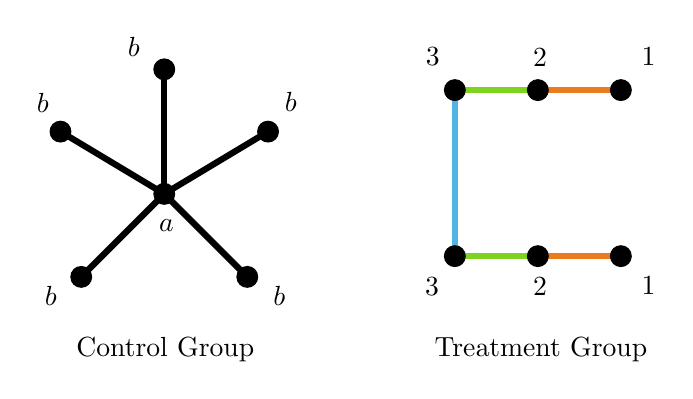
\begin{tikzpicture}[x=0.75pt,y=0.75pt,yscale=-1,xscale=1]
	%uncomment if require: \path (0,242); %set diagram left start at 0, and has height of 242
	
	%Straight Lines [id:da8360249781061426] 
	\draw [color={rgb, 255:red, 235; green, 124; blue, 29 }  ,draw opacity=1 ][line width=2.25]    (285,155) -- (325,155) ;
	%Straight Lines [id:da8158257704190623] 
	\draw [color={rgb, 255:red, 235; green, 124; blue, 29 }  ,draw opacity=1 ][line width=2.25]    (285,75) -- (325,75) ;
	%Straight Lines [id:da7285129998191696] 
	\draw [line width=2.25]    (105,65) -- (105,125) ;
	%Straight Lines [id:da1945257120538626] 
	\draw [line width=2.25]    (65,165) -- (105,125) ;
	%Straight Lines [id:da15064502001286517] 
	\draw [line width=2.25]    (105,125) -- (145,165) ;
	%Straight Lines [id:da8625361583469673] 
	\draw [color={rgb, 255:red, 126; green, 211; blue, 33 }  ,draw opacity=1 ][line width=2.25]    (245,75) -- (285,75) ;
	%Straight Lines [id:da8513199064736671] 
	\draw [color={rgb, 255:red, 126; green, 211; blue, 33 }  ,draw opacity=1 ][line width=2.25]    (245,155) -- (285,155) ;
	%Straight Lines [id:da5064308868951334] 
	\draw [color={rgb, 255:red, 80; green, 181; blue, 227 }  ,draw opacity=1 ][line width=2.25]    (245,75) -- (245,155) ;
	%Shape: Circle [id:dp7020190518871161] 
	\draw  [fill={rgb, 255:red, 0; green, 0; blue, 0 }  ,fill opacity=1 ] (100,65) .. controls (100,62.24) and (102.24,60) .. (105,60) .. controls (107.76,60) and (110,62.24) .. (110,65) .. controls (110,67.76) and (107.76,70) .. (105,70) .. controls (102.24,70) and (100,67.76) .. (100,65) -- cycle ;
	%Shape: Circle [id:dp4472245437398714] 
	\draw  [fill={rgb, 255:red, 0; green, 0; blue, 0 }  ,fill opacity=1 ] (100,125) .. controls (100,122.24) and (102.24,120) .. (105,120) .. controls (107.76,120) and (110,122.24) .. (110,125) .. controls (110,127.76) and (107.76,130) .. (105,130) .. controls (102.24,130) and (100,127.76) .. (100,125) -- cycle ;
	%Shape: Circle [id:dp332527728107481] 
	\draw  [fill={rgb, 255:red, 0; green, 0; blue, 0 }  ,fill opacity=1 ] (60,165) .. controls (60,162.24) and (62.24,160) .. (65,160) .. controls (67.76,160) and (70,162.24) .. (70,165) .. controls (70,167.76) and (67.76,170) .. (65,170) .. controls (62.24,170) and (60,167.76) .. (60,165) -- cycle ;
	%Shape: Circle [id:dp5070907001685069] 
	\draw  [fill={rgb, 255:red, 0; green, 0; blue, 0 }  ,fill opacity=1 ] (140,165) .. controls (140,162.24) and (142.24,160) .. (145,160) .. controls (147.76,160) and (150,162.24) .. (150,165) .. controls (150,167.76) and (147.76,170) .. (145,170) .. controls (142.24,170) and (140,167.76) .. (140,165) -- cycle ;
	%Shape: Circle [id:dp7312361016882203] 
	\draw  [fill={rgb, 255:red, 0; green, 0; blue, 0 }  ,fill opacity=1 ] (240,75) .. controls (240,72.24) and (242.24,70) .. (245,70) .. controls (247.76,70) and (250,72.24) .. (250,75) .. controls (250,77.76) and (247.76,80) .. (245,80) .. controls (242.24,80) and (240,77.76) .. (240,75) -- cycle ;
	%Shape: Circle [id:dp6877519316777763] 
	\draw  [fill={rgb, 255:red, 0; green, 0; blue, 0 }  ,fill opacity=1 ] (320,75) .. controls (320,72.24) and (322.24,70) .. (325,70) .. controls (327.76,70) and (330,72.24) .. (330,75) .. controls (330,77.76) and (327.76,80) .. (325,80) .. controls (322.24,80) and (320,77.76) .. (320,75) -- cycle ;
	%Shape: Circle [id:dp21492882036619276] 
	\draw  [fill={rgb, 255:red, 0; green, 0; blue, 0 }  ,fill opacity=1 ] (320,155) .. controls (320,152.24) and (322.24,150) .. (325,150) .. controls (327.76,150) and (330,152.24) .. (330,155) .. controls (330,157.76) and (327.76,160) .. (325,160) .. controls (322.24,160) and (320,157.76) .. (320,155) -- cycle ;
	%Shape: Circle [id:dp1595771278608995] 
	\draw  [fill={rgb, 255:red, 0; green, 0; blue, 0 }  ,fill opacity=1 ] (240,155) .. controls (240,152.24) and (242.24,150) .. (245,150) .. controls (247.76,150) and (250,152.24) .. (250,155) .. controls (250,157.76) and (247.76,160) .. (245,160) .. controls (242.24,160) and (240,157.76) .. (240,155) -- cycle ;
	%Straight Lines [id:da9822349173412578] 
	\draw [line width=2.25]    (105,125) -- (155,95) ;
	%Shape: Circle [id:dp7709379434514961] 
	\draw  [fill={rgb, 255:red, 0; green, 0; blue, 0 }  ,fill opacity=1 ] (150,95) .. controls (150,92.24) and (152.24,90) .. (155,90) .. controls (157.76,90) and (160,92.24) .. (160,95) .. controls (160,97.76) and (157.76,100) .. (155,100) .. controls (152.24,100) and (150,97.76) .. (150,95) -- cycle ;
	%Shape: Circle [id:dp9939137807167766] 
	\draw  [fill={rgb, 255:red, 0; green, 0; blue, 0 }  ,fill opacity=1 ] (50,95) .. controls (50,92.24) and (52.24,90) .. (55,90) .. controls (57.76,90) and (60,92.24) .. (60,95) .. controls (60,97.76) and (57.76,100) .. (55,100) .. controls (52.24,100) and (50,97.76) .. (50,95) -- cycle ;
	%Straight Lines [id:da9699796513691362] 
	\draw [line width=2.25]    (55,95) -- (105,125) ;
	%Shape: Circle [id:dp9943805701380365] 
	\draw  [fill={rgb, 255:red, 0; green, 0; blue, 0 }  ,fill opacity=1 ] (280,75) .. controls (280,72.24) and (282.24,70) .. (285,70) .. controls (287.76,70) and (290,72.24) .. (290,75) .. controls (290,77.76) and (287.76,80) .. (285,80) .. controls (282.24,80) and (280,77.76) .. (280,75) -- cycle ;
	%Shape: Circle [id:dp0350269156660592] 
	\draw  [fill={rgb, 255:red, 0; green, 0; blue, 0 }  ,fill opacity=1 ] (280,155) .. controls (280,152.24) and (282.24,150) .. (285,150) .. controls (287.76,150) and (290,152.24) .. (290,155) .. controls (290,157.76) and (287.76,160) .. (285,160) .. controls (282.24,160) and (280,157.76) .. (280,155) -- cycle ;
	
	% Text Node
	\draw (106,140.5) node   [align=left] {$\displaystyle a$};
	% Text Node
	\draw (90.38,54) node   [align=left] {$\displaystyle b$};
	% Text Node
	\draw (50.38,174) node   [align=left] {$\displaystyle b$};
	% Text Node
	\draw (160.38,174) node   [align=left] {$\displaystyle b$};
	% Text Node
	\draw (234.38,59) node   [align=left] {$\displaystyle 3$};
	% Text Node
	\draw (234,169.5) node   [align=left] {$\displaystyle 3$};
	% Text Node
	\draw (338.38,169) node   [align=left] {$\displaystyle 1$};
	% Text Node
	\draw (338.38,59) node   [align=left] {$\displaystyle 1$};
	% Text Node
	\draw (286.5,200) node   [align=left] {Treatment Group};
	% Text Node
	\draw (105.5,200) node   [align=left] {Control Group};
	% Text Node
	\draw (286,59.5) node   [align=left] {$\displaystyle 2$};
	% Text Node
	\draw (286,169.5) node   [align=left] {$\displaystyle 2$};
	% Text Node
	\draw (166,80.5) node   [align=left] {$\displaystyle b$};
	% Text Node
	\draw (46.5,81) node   [align=left] {$\displaystyle b$};
	
	
\end{tikzpicture}
\vspace{-6mm}
\caption{A toy example of an experiment. The six agents assigned to the treatment group form a line under the new policy. The six agents assigned to the control group form a star under the status quo.}
\label{fig:toyexample_problem}
\end{figure}

\subsection{The main identification assumption}
Our first main contribution is to propose a condition that formalizes how the random assignment of agents to groups refines the identified set. Our main identification assumption is that $Y_{0}(1)$ and $Y_{1}(1)$ are \emph{weakly isomorphic}. We defer a formal definition of this assumption to Section 4.1, but, intuitively, it says that the configuration of network connections between agents assigned to the treatment group describe how the agents assigned to the control group would be connected if that group were assigned the new policy instead of the status quo. This assumption is a network analog of the conventional assumption that the entries of $Y_{0}(1)$ and $Y_{1}(1)$ have the same empirical distribution, which is a strong but ubiquitous implication of random assignment, see Chapter 7.3 of \cite{manski2009identification} for a textbook discussion. \looseness=-1

As in a conventional experiment, randomization only generally implies that $Y_{0}(1)$ and $Y_{1}(1)$ are weakly isomorphic in expectation. However, to illustrate the main identification problem of our paper, we will, for this simplified illustration, make the strong and unrealistic assumption that it holds exactly in the realized experiment.  \looseness=-1  

Formally, the main identification assumption is that there exists an $N\times N$ permutation matrix $\Pi$,\footnote{A permutation matrix is a square matrix with $\{0,1\}$-valued entries. Every row and column sums to $1$.} unknown to the researcher, such that  \looseness=-1 
\begin{align}\label{simAss}
Y_{ij,0}(1) = \sum_{k,l=1}^{N}Y_{kl,1}(1)\Pi_{ik}\Pi_{jl}.
\end{align}
In words, condition (\ref{simAss}) says that there exists a one-to-one match between agents in the two groups such that the counterfactual outcomes of the agents in group $0$ are given by their matches in group $1$. It could be rationalized by a specific experimental design conducted on $N$ pairs or ``clones'' of agents. One member of each pair is randomly assigned to each group and the counterfactual connection between agents in the control group is given by their clones in the treatment group. If the researcher knows which pairs of agents are clones, then they can  compute (\ref{param}) by simply substituting $Y_{ij,0}(1)$ with $Y_{c_{i}c_{j},1}(1)$ where $c_{i}$ is the identity of $i$'s clone. But the researcher has forgotten this information so that, in principle, any matching between the agents of the treatment and control groups (as represented by some permutation matrix) could be the correct one.  \looseness=-1  

If the researcher conducts such a clone experiment, then  (\ref{simAss}) holds exactly in a finite sample. However, outside this specific setting, randomization does not generally imply this condition.  Instead, it is an approximation to what randomization does in large samples. The idea that randomization can be characterized by an approximate matching is not original to our paper: an analogous condition plays a key role in the identification arguments of the Fr\'echet-Hoeffding-Makarov bounds and quantile treatment effects literature. See \cite{whitt1976bivariate,heckman1997making} for detailed discussions. What is new in our setting is that the quadratic structure of (\ref{simAss}) makes the problem of identifying social disruption with network data fundamentally different. We discuss this complication in Section 2.2.2 below.   \looseness=-1  


\subsubsection{The identified set under the main identification assumption}
Though condition (\ref{simAss}) is intended to be an approximation, to illustrate its identifying content in this section we suppose that it holds exactly. Plugging (\ref{simAss}) into (\ref{param}) implies that the number of links destroyed by the policy is \looseness=-1  
\begin{align*}
\frac{1}{2}\sum_{i,j = 1}^{N}(1-Y_{ij,0}(1))Y_{ij,0}(0) = \frac{1}{2}\sum_{i,j,k,l = 1}^{N}(1-Y_{kl,1}(1))Y_{ij,0}(0)\Pi_{ik}\Pi_{jl}.
\end{align*}
The substitution solves the initial problem that $Y_{0}(1)$ is not known because both $Y_{1}(1)$ and $Y_{0}(0)$ on the right-hand side are observed. However, the right-hand side now depends on the unknown $\Pi$. Since, under (\ref{simAss}), any permutation matrix suggests a number of destroyed links that is consistent with the observed network connections, the identified set is \looseness=-1  
 \begin{align}\label{paramset2}
 \left\{\theta \in \mathbb{N}: \theta = \frac{1}{2}\sum_{i,j,k,l = 1}^{N}(1-Y_{kl,1}(1))Y_{ij,0}(0)P_{ik}P_{jl} \text{ for any permutation matrix } P \right\}.
 \end{align}


\begin{myexpcont}
In the toy example, condition (\ref{simAss}) implies that if the new policy were implemented in the control group, the agents would change their social connections to form a line. Under this assumption, the identified set for the number of connections destroyed by the policy is $\{3,4\}$. The logic behind this result is illustrated in Figure 2. There are three ways up to symmetry to match the six agents in the control group to the six agents in the treatment group. Matching  $a$ in the control group to position $1$ in the treatment group destroys four connections. This is because all five connections are adjacent to $a$ in the control group and $1$ has only one connection in the treatment group. Similarly, matching $a$ to positions $2$ or $3$ destroys three connections. Since these are the only unique matches up to a relabeling of the agents, the policy must destroy 3 or 4 out of 5 connections ($60$ or $80$ percent). It follows that, under  (\ref{simAss}), this example necessarily has a large amount of social disruption. \looseness=-1  
\end{myexpcont}

\begin{figure}
\centering


\tikzset{every picture/.style={line width=0.75pt}} %set default line width to 0.75pt        

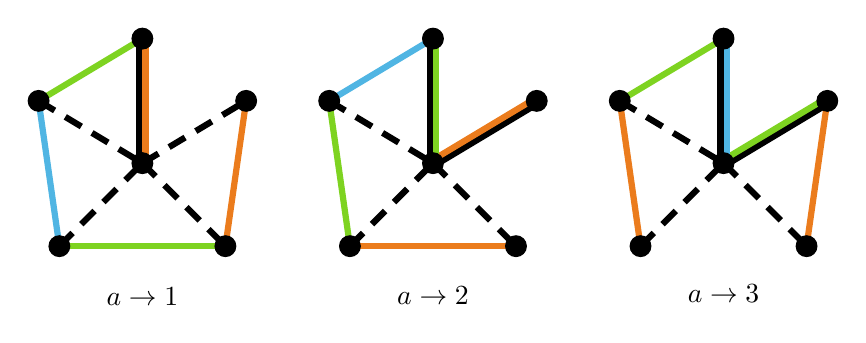
\begin{tikzpicture}[x=0.75pt,y=0.75pt,yscale=-1,xscale=1]
	%uncomment if require: \path (0,242); %set diagram left start at 0, and has height of 242
	
	%Straight Lines [id:da6006307035883517] 
	\draw [color={rgb, 255:red, 235; green, 124; blue, 29 }  ,draw opacity=1 ][line width=2.25]    (315,165) -- (305,95) ;
	%Straight Lines [id:da2628452665477662] 
	\draw [line width=2.25]    (216,126) -- (266,96) ;
	%Straight Lines [id:da7867605309196273] 
	\draw [color={rgb, 255:red, 235; green, 124; blue, 29 }  ,draw opacity=1 ][line width=2.25]    (214,124) -- (264,94) ;
	%Straight Lines [id:da20974090082161245] 
	\draw [color={rgb, 255:red, 235; green, 124; blue, 29 }  ,draw opacity=1 ][line width=2.25]    (125,95) -- (115,165) ;
	%Straight Lines [id:da3642708459455063] 
	\draw [color={rgb, 255:red, 126; green, 211; blue, 33 }  ,draw opacity=1 ][line width=2.25]    (35,165) -- (115,165) ;
	%Straight Lines [id:da2510429813427911] 
	\draw [color={rgb, 255:red, 80; green, 181; blue, 227 }  ,draw opacity=1 ][line width=2.25]    (35,165) -- (25,95) ;
	%Straight Lines [id:da26518610675394505] 
	\draw [color={rgb, 255:red, 126; green, 211; blue, 33 }  ,draw opacity=1 ][line width=2.25]    (25,95) -- (75,65) ;
	%Straight Lines [id:da15555504660860886] 
	\draw [line width=2.25]    (73.5,65) -- (73.5,125) ;
	%Straight Lines [id:da9319742594731747] 
	\draw [color={rgb, 255:red, 235; green, 124; blue, 29 }  ,draw opacity=1 ][line width=2.25]    (76.5,65) -- (76.5,125) ;
	%Straight Lines [id:da5351968154129055] 
	\draw [line width=2.25]  [dash pattern={on 6.75pt off 4.5pt}]  (35,165) -- (75,125) ;
	%Straight Lines [id:da2677247736086712] 
	\draw [line width=2.25]  [dash pattern={on 6.75pt off 4.5pt}]  (75,125) -- (115,165) ;
	%Shape: Circle [id:dp2822714540066722] 
	\draw  [fill={rgb, 255:red, 0; green, 0; blue, 0 }  ,fill opacity=1 ] (70,65) .. controls (70,62.24) and (72.24,60) .. (75,60) .. controls (77.76,60) and (80,62.24) .. (80,65) .. controls (80,67.76) and (77.76,70) .. (75,70) .. controls (72.24,70) and (70,67.76) .. (70,65) -- cycle ;
	%Shape: Circle [id:dp8647332015586298] 
	\draw  [fill={rgb, 255:red, 0; green, 0; blue, 0 }  ,fill opacity=1 ] (70,125) .. controls (70,122.24) and (72.24,120) .. (75,120) .. controls (77.76,120) and (80,122.24) .. (80,125) .. controls (80,127.76) and (77.76,130) .. (75,130) .. controls (72.24,130) and (70,127.76) .. (70,125) -- cycle ;
	%Shape: Circle [id:dp9341805611726252] 
	\draw  [fill={rgb, 255:red, 0; green, 0; blue, 0 }  ,fill opacity=1 ] (30,165) .. controls (30,162.24) and (32.24,160) .. (35,160) .. controls (37.76,160) and (40,162.24) .. (40,165) .. controls (40,167.76) and (37.76,170) .. (35,170) .. controls (32.24,170) and (30,167.76) .. (30,165) -- cycle ;
	%Shape: Circle [id:dp6347309455271312] 
	\draw  [fill={rgb, 255:red, 0; green, 0; blue, 0 }  ,fill opacity=1 ] (110,165) .. controls (110,162.24) and (112.24,160) .. (115,160) .. controls (117.76,160) and (120,162.24) .. (120,165) .. controls (120,167.76) and (117.76,170) .. (115,170) .. controls (112.24,170) and (110,167.76) .. (110,165) -- cycle ;
	%Straight Lines [id:da2354506575862637] 
	\draw [line width=2.25]  [dash pattern={on 6.75pt off 4.5pt}]  (75,125) -- (125,95) ;
	%Shape: Circle [id:dp27440282635206015] 
	\draw  [fill={rgb, 255:red, 0; green, 0; blue, 0 }  ,fill opacity=1 ] (120,95) .. controls (120,92.24) and (122.24,90) .. (125,90) .. controls (127.76,90) and (130,92.24) .. (130,95) .. controls (130,97.76) and (127.76,100) .. (125,100) .. controls (122.24,100) and (120,97.76) .. (120,95) -- cycle ;
	%Shape: Circle [id:dp2742824203776172] 
	\draw  [fill={rgb, 255:red, 0; green, 0; blue, 0 }  ,fill opacity=1 ] (20,95) .. controls (20,92.24) and (22.24,90) .. (25,90) .. controls (27.76,90) and (30,92.24) .. (30,95) .. controls (30,97.76) and (27.76,100) .. (25,100) .. controls (22.24,100) and (20,97.76) .. (20,95) -- cycle ;
	%Straight Lines [id:da5792134404795799] 
	\draw [line width=2.25]  [dash pattern={on 6.75pt off 4.5pt}]  (25,95) -- (75,125) ;
	%Straight Lines [id:da9688758191181335] 
	\draw [color={rgb, 255:red, 235; green, 124; blue, 29 }  ,draw opacity=1 ][line width=2.25]    (175,165) -- (255,165) ;
	%Straight Lines [id:da32600537898081305] 
	\draw [color={rgb, 255:red, 126; green, 211; blue, 33 }  ,draw opacity=1 ][line width=2.25]    (175,165) -- (165,95) ;
	%Straight Lines [id:da8779003930009404] 
	\draw [color={rgb, 255:red, 80; green, 181; blue, 227 }  ,draw opacity=1 ][line width=2.25]    (165,95) -- (215,65) ;
	%Straight Lines [id:da9721333086578243] 
	\draw [line width=2.25]    (213.5,65) -- (213.5,125) ;
	%Straight Lines [id:da2605254490006198] 
	\draw [color={rgb, 255:red, 126; green, 211; blue, 33 }  ,draw opacity=1 ][line width=2.25]    (216.5,65) -- (216.5,125) ;
	%Straight Lines [id:da3689463172698282] 
	\draw [line width=2.25]  [dash pattern={on 6.75pt off 4.5pt}]  (175,165) -- (215,125) ;
	%Straight Lines [id:da3422067536965029] 
	\draw [line width=2.25]  [dash pattern={on 6.75pt off 4.5pt}]  (215,125) -- (255,165) ;
	%Shape: Circle [id:dp41630836475307786] 
	\draw  [fill={rgb, 255:red, 0; green, 0; blue, 0 }  ,fill opacity=1 ] (210,65) .. controls (210,62.24) and (212.24,60) .. (215,60) .. controls (217.76,60) and (220,62.24) .. (220,65) .. controls (220,67.76) and (217.76,70) .. (215,70) .. controls (212.24,70) and (210,67.76) .. (210,65) -- cycle ;
	%Shape: Circle [id:dp2563859670613374] 
	\draw  [fill={rgb, 255:red, 0; green, 0; blue, 0 }  ,fill opacity=1 ] (210,125) .. controls (210,122.24) and (212.24,120) .. (215,120) .. controls (217.76,120) and (220,122.24) .. (220,125) .. controls (220,127.76) and (217.76,130) .. (215,130) .. controls (212.24,130) and (210,127.76) .. (210,125) -- cycle ;
	%Shape: Circle [id:dp38765623270360516] 
	\draw  [fill={rgb, 255:red, 0; green, 0; blue, 0 }  ,fill opacity=1 ] (170,165) .. controls (170,162.24) and (172.24,160) .. (175,160) .. controls (177.76,160) and (180,162.24) .. (180,165) .. controls (180,167.76) and (177.76,170) .. (175,170) .. controls (172.24,170) and (170,167.76) .. (170,165) -- cycle ;
	%Shape: Circle [id:dp9846560578580156] 
	\draw  [fill={rgb, 255:red, 0; green, 0; blue, 0 }  ,fill opacity=1 ] (250,165) .. controls (250,162.24) and (252.24,160) .. (255,160) .. controls (257.76,160) and (260,162.24) .. (260,165) .. controls (260,167.76) and (257.76,170) .. (255,170) .. controls (252.24,170) and (250,167.76) .. (250,165) -- cycle ;
	%Shape: Circle [id:dp2066269183286572] 
	\draw  [fill={rgb, 255:red, 0; green, 0; blue, 0 }  ,fill opacity=1 ] (260,95) .. controls (260,92.24) and (262.24,90) .. (265,90) .. controls (267.76,90) and (270,92.24) .. (270,95) .. controls (270,97.76) and (267.76,100) .. (265,100) .. controls (262.24,100) and (260,97.76) .. (260,95) -- cycle ;
	%Shape: Circle [id:dp8550081914236752] 
	\draw  [fill={rgb, 255:red, 0; green, 0; blue, 0 }  ,fill opacity=1 ] (160,95) .. controls (160,92.24) and (162.24,90) .. (165,90) .. controls (167.76,90) and (170,92.24) .. (170,95) .. controls (170,97.76) and (167.76,100) .. (165,100) .. controls (162.24,100) and (160,97.76) .. (160,95) -- cycle ;
	%Straight Lines [id:da6619397439718806] 
	\draw [line width=2.25]  [dash pattern={on 6.75pt off 4.5pt}]  (165,95) -- (215,125) ;
	%Straight Lines [id:da9059214036659999] 
	\draw [line width=2.25]    (356,126) -- (406,96) ;
	%Straight Lines [id:da8645812492079664] 
	\draw [color={rgb, 255:red, 126; green, 211; blue, 33 }  ,draw opacity=1 ][line width=2.25]    (354,124) -- (404,94) ;
	%Straight Lines [id:da4938950823293964] 
	\draw [color={rgb, 255:red, 235; green, 124; blue, 29 }  ,draw opacity=1 ][line width=2.25]    (395,165) -- (405,95) ;
	%Straight Lines [id:da22293897667086415] 
	\draw [color={rgb, 255:red, 126; green, 211; blue, 33 }  ,draw opacity=1 ][line width=2.25]    (305,95) -- (355,65) ;
	%Straight Lines [id:da14611318194757272] 
	\draw [line width=2.25]    (353.5,65) -- (353.5,125) ;
	%Straight Lines [id:da894025729827258] 
	\draw [color={rgb, 255:red, 80; green, 181; blue, 227 }  ,draw opacity=1 ][line width=2.25]    (356.5,65) -- (356.5,125) ;
	%Straight Lines [id:da45572091002799753] 
	\draw [line width=2.25]  [dash pattern={on 6.75pt off 4.5pt}]  (315,165) -- (355,125) ;
	%Straight Lines [id:da08311770578305777] 
	\draw [line width=2.25]  [dash pattern={on 6.75pt off 4.5pt}]  (355,125) -- (395,165) ;
	%Shape: Circle [id:dp6752324712932157] 
	\draw  [fill={rgb, 255:red, 0; green, 0; blue, 0 }  ,fill opacity=1 ] (350,65) .. controls (350,62.24) and (352.24,60) .. (355,60) .. controls (357.76,60) and (360,62.24) .. (360,65) .. controls (360,67.76) and (357.76,70) .. (355,70) .. controls (352.24,70) and (350,67.76) .. (350,65) -- cycle ;
	%Shape: Circle [id:dp6752078925235562] 
	\draw  [fill={rgb, 255:red, 0; green, 0; blue, 0 }  ,fill opacity=1 ] (350,125) .. controls (350,122.24) and (352.24,120) .. (355,120) .. controls (357.76,120) and (360,122.24) .. (360,125) .. controls (360,127.76) and (357.76,130) .. (355,130) .. controls (352.24,130) and (350,127.76) .. (350,125) -- cycle ;
	%Shape: Circle [id:dp4226149077098045] 
	\draw  [fill={rgb, 255:red, 0; green, 0; blue, 0 }  ,fill opacity=1 ] (310,165) .. controls (310,162.24) and (312.24,160) .. (315,160) .. controls (317.76,160) and (320,162.24) .. (320,165) .. controls (320,167.76) and (317.76,170) .. (315,170) .. controls (312.24,170) and (310,167.76) .. (310,165) -- cycle ;
	%Shape: Circle [id:dp8573155868089057] 
	\draw  [fill={rgb, 255:red, 0; green, 0; blue, 0 }  ,fill opacity=1 ] (390,165) .. controls (390,162.24) and (392.24,160) .. (395,160) .. controls (397.76,160) and (400,162.24) .. (400,165) .. controls (400,167.76) and (397.76,170) .. (395,170) .. controls (392.24,170) and (390,167.76) .. (390,165) -- cycle ;
	%Shape: Circle [id:dp7646452787565435] 
	\draw  [fill={rgb, 255:red, 0; green, 0; blue, 0 }  ,fill opacity=1 ] (400,95) .. controls (400,92.24) and (402.24,90) .. (405,90) .. controls (407.76,90) and (410,92.24) .. (410,95) .. controls (410,97.76) and (407.76,100) .. (405,100) .. controls (402.24,100) and (400,97.76) .. (400,95) -- cycle ;
	%Shape: Circle [id:dp9138095748049607] 
	\draw  [fill={rgb, 255:red, 0; green, 0; blue, 0 }  ,fill opacity=1 ] (300,95) .. controls (300,92.24) and (302.24,90) .. (305,90) .. controls (307.76,90) and (310,92.24) .. (310,95) .. controls (310,97.76) and (307.76,100) .. (305,100) .. controls (302.24,100) and (300,97.76) .. (300,95) -- cycle ;
	%Straight Lines [id:da5227884975676973] 
	\draw [line width=2.25]  [dash pattern={on 6.75pt off 4.5pt}]  (305,95) -- (355,125) ;
	
	% Text Node
	\draw (75,189.5) node    {$a \rightarrow 1$};
	% Text Node
	\draw (215,189) node    {$a \rightarrow 2$};
	% Text Node
	\draw (355,188) node    {$a \rightarrow 3$};
	
	
\end{tikzpicture}
\vspace{-6mm}
\caption{There are three ways to match agents in the control group to the treatment group up to symmetry. A black dashed line indicates a destroyed connection. It exists under the status quo but not the new policy. A colored and a black solid line indicates a maintained connection. It exists under both the status quo and the new policy. A colored line only indicates a created connection. It exists under the new policy but not the status quo.}
\label{fig:toyexample_matrix}
\end{figure}




\subsubsection{The identified set is typically uncomputable}
It is straightforward to compute the identified set (\ref{paramset2}) in our toy example because $N$ is small. However, computing the identified set is not possible in many cases of interest. This is because the problem of finding the largest or smallest element of (\ref{paramset2}) is equivalent to solving a quadratic assignment problem which is strongly NP hard in theory and practically uncomputable for instances with more than a few dozen agents. See Section 1.5 of \cite{cela2013quadratic}.  \looseness=-1  

Our second main contribution is to instead propose tractable outer bounds that are both informative about social disruption and computationally feasible even for large networks. Intuitively, it is hard to compute sharp bounds on  (\ref{paramset2}) because searching over permutation matrices is difficult. Our bounds instead search over orthogonal matrices.\footnote{An orthogonal matrix is a square matrix where the inner product of any row or column with itself is $1$ and the inner product of any two distinct rows or two distinct columns is $0$.} To illustrate this idea, we replace (\ref{paramset2}) with 
 \begin{align}\label{paramset3}
 \left\{\theta \in \mathbb{N}: \theta = \frac{1}{2}\sum_{i,j,k,l = 1}^{N}(1-Y_{kl,1}(1))Y_{ij,0}(0)O_{ik}O_{jl} \text{ for any orthogonal matrix } O \right\}.
 \end{align}
There are two reasons for this substitution. First, because all permutation matrices are orthogonal, (\ref{paramset3}) contains (\ref{paramset2}) and so any bounds on (\ref{paramset3})  will also be valid for (\ref{paramset2}). Second, solving for the smallest and largest element of (\ref{paramset3})  is relatively straightforward: the minimum is $\sum_{r=1}^{N}\lambda_{r}(1)\lambda_{N-r}(0)$ and the maximum is  $\sum_{r=1}^{N}\lambda_{r}(1)\lambda_{r}(0)$ where $\lambda_{r}(s)$ is the $r$th largest eigenvalue of $(1-Y_{s}(s))^{s}Y_{s}(s)^{1-s}$. See Lemma 2 in Appendix Section A.3 for a proof.\footnote{The idea of bounding a QAP by searching over orthogonal matrices was originally proposed by \cite{finke1987quadratic}, however applying this logic to our general setting is not straightforward and requires arguments not typical of the QAP literature. See Section 4.1 for a discussion. } \looseness=-1  


\subsubsection{Our bounds can be more informative than conventional methods}
Conventional methods such as computing the difference in the number of connections or the Fr\'echet-Hoeffding bounds are not generally effective at identifying social disruption.\footnote{Typically the literature runs dyadic regressions. They regress the magnitude of the connection between a pair of agents on an indicator for whether the agents are subjected to the new policy and additional covariates. The coefficient on the policy indicator is then used to measure social disruption. Without covariates, this is equivalent to computing the difference in the number of connections. Including covariates does not generally make these regressions informative about social disruption. See our empirical illustration in Section 6.} The difference in the number of connections, $\frac{1}{2}\sum_{i,j = 1}^{N}Y_{ij,0}(0) - \frac{1}{2}\sum_{i,j = 1}^{N}Y_{ij,1}(1)$, is also the number of connections destroyed by the new policy minus the number of connections created. It is only a good approximation of the number of destroyed connections if the number of created connections is close to zero, which is rare in practice.  \looseness=-1 

The Fr\'echet-Hoeffding  lower bound on (\ref{param}) is $\max(\frac{1}{2}\sum_{i,j=1}^{N}Y_{ij,0}(0)- \frac{1}{2}\sum_{i,j=1}^{N}Y_{ij,1}(1),0)$. The upper bound is $\min(\frac{1}{2}\sum_{i,j=1}^{N}(1-Y_{ij,1}(1)),\frac{1}{2}\sum_{i,j=1}^{N}Y_{ij,0}(0))$. These bounds are valid in that the number of destroyed connections is necessarily between them, but they are not generally informative. The lower bound is essentially the difference in the number of connections and is zero if the policy creates at least as many connections as it destroys. The upper bound is large if there are many pairs of agents that are connected in the control group and many pairs of agents that are not connected in the treatment group. Both are common in practice.  \looseness=-1 

The problem with these methods is that they do not use all of the information available in condition (\ref{simAss}). They only use the relatively weak implication that $Y_{0}(1)$ and $Y_{1}(1)$ have the same number of connections. Our bounds often perform better because there can be important identifying information in the former restriction that is not in the latter. \looseness=-1  



\begin{myexpcont}
Neither conventional method described in Section 2.2.3 is informative about social disruption in the toy example. The difference in the number of connections between treatment groups is $5 - 5 = 0$, which does not identify any social disruption. The upper Fr\'echet-Hoeffding bound is $\min(5,10) = 5$ and the lower bound is $5 - 5 = 0$, which are equivalent to the trivial bounds derived in Section 2.1.1 that do not use condition (\ref{simAss}). \looseness=-1 

Our bounds, in contrast, give an upper bound of 4.17 and a lower bound of 1.6.\footnote{These bounds are in Proposition 2 of Section 5.2 and use the adjustment in Online Appendix Section  D.2. They are implemented in an R package available at \url{https://github.com/yong-cai/MatrixHTE}.} They imply that the number of destroyed links belongs to $\{2,3,4\}$ which is close to the identified set of $\{3,4\}$ derived in Section 2.2.2. In particular, our bounds imply that the fraction of destroyed links is between $40$ and $80$ percent, which is not quite the sharp bounds of $60$ and $80$ percent, but is a substantial improvement on the conventional/trivial bounds of $0$ and $100$ percent. \looseness=-1 \end{myexpcont}

The performance of our methodology is not limited to the toy example. Section 6 provides empirical evidence showing that our bounds can be much more effective at identifying social disruption than conventional methods in a real world setting.\looseness=-1 

%\subsection{From identification to estimation and inference}
%In practice, researchers often model the network connections between agents as random. For example, a common specification in the literature is the nonlinear dyadic regression model \looseness=-1 \begin{align*}
%Y_{ij,s}(s) = \Lambda\left(X_{ij,s}\beta_s \right) + \varepsilon_{ij,s}
%\end{align*} 
%where $\Lambda$ is a known link function such as the identity or logistic function, $X$ are observed characteristics,  $\varepsilon$ has weakly dependent mean-zero entries that are mean independent of $X$ and independent across treatment groups. 
%
%When the outcomes are random, a potential parameter of interest is the expected number of connections that would be destroyed by implementing the new policy in the control group. Under condition (\ref{simAss}), this parameter of interest is given by \looseness=-1 
%\begin{align*}
%\mathbb{E}\left[\frac{1}{2}\sum_{i,j = 1}^{N}(1-Y_{ij,0}(1))Y_{ij,0}(0)\right] 
%= \frac{1}{2}\sum_{i,j,k,l = 1}^{N}\left(1 - \Lambda\left(X_{kl,1}\beta_1\right)\right)\Lambda\left(X_{ij,0}\beta_0\right)\Pi_{ik}\Pi_{jl}
%\end{align*}
%where the expectation $\mathbb{E}$ is taken with respect to the error $\varepsilon_{ij,t}$ conditional on $X_{ij,t}$ . \looseness=-1 
%
%The researcher can then apply the identification logic of Section 2.2 to the matrices $\Lambda\left(X_{1}\beta_1\right)$ and  $\Lambda\left(X_{0}\beta_0\right)$, and derive the bounds $\sum_{r=1}^{N}\rho_r(1)\rho_{N-r}(0)$ and $\sum_{r=1}^{N}\rho_r(1)\rho_{r}(0)$ where $\rho_{r}(t)$ is the $r$th largest eigenvalue of $(1-\Lambda\left(X_{1}\beta_1\right))^{t}\Lambda\left(X_{0}\beta_0\right)^{1-t}$. In this case, the eigenvalue $\rho_{r}(t)$ cannot be directly computed because $\beta_0$ and $\beta_1$ are not known. A natural way to estimate $\rho_{r}(t)$ is to first compute $\hat{\beta}_0$ and $\hat{\beta}_1$ by least squares and then estimate the eigenvalues of $\left(1-\Lambda\left(X_{1}\beta_1\right)\right)^{t}\Lambda\left(X_{0}\beta_0\right)^{1-t}$ using those of $\left(1-\Lambda\left(X_{1}\hat{\beta}_1\right)\right)^{t}\Lambda\left(X_{0}\hat{\beta}_0\right)^{1-t}$. We construct valid confidence intervals using this estimation strategy in Online Appendix Section D.3.  \looseness=-1  

  
\section{Main framework}
In this section, we describe our framework. We first define the parameters of interest and then specify a model for the data. We focus on undirected networks, i.e. networks that can be represented by a symmetric real-valued adjacency matrix. The framework and results immediately extended to the directed case by a symmetrization argument described in Online Appendix Section D.1. This use of symmetrization to extend results from the symmetric case to the asymmetric case is standard and comes from the literature on U-statistics. See, for instance, Section 5.1.1 of \cite{serfling2009approximation} for a textbook presentation.  \looseness=-1 

\subsection{Potential outcomes and the parameters of interest}
\subsubsection{Potential outcomes}
A community of $N$ agents may be subjected to one of two policies indexed by $s \in \{0,1\}$. In our framework, we use the word ``policy'' to refer to any community-level intervention that influences the network connections between agents. One policy could, for instance, assign an individualized treatment to every agent in the community. Another policy could assign the treatment to a subpopulation of agents. Still another policy could be the introduction of a public good that is available to all members of the community. All of these examples fall within our framework.  \looseness=-1 

Once the community is subjected to one of the two policies, the agents interact and form connections. For two arbitrary agents $i$ and $j$ in the community, the variable $Y_{ij}(s)$ describes the magnitude of the connection between agents $i$ and $j$ when the community is assigned policy $s$. We refer to these quantities as potential outcomes or potential connections. \looseness=-1 

\begin{remark}
When the policy concerns the assignment of an individualized treatment to agents in the community, our framework does not rule out treatment spillovers, but it does not explicitly model them either. Similarly, our framework neither rules out nor explicitly models strategic interactions between agents in the community. We discuss the sense in which treatment spillovers and strategic interactions are accommodated after we introduce our parameters of interest (Section 3.1.2) and model (Sections 3.2.2) below.\looseness=-1 
\end{remark}

\subsubsection{Parameters of interest}
We focus on the joint distribution of potential outcomes (DPO): \looseness=-1 
\begin{align}\label{joint}
F(y_{1},y_{0}) := \mathbb{P}\left(Y_{ij}(1)  \leq y_1, Y_{ij}(0)  \leq y_{0}\right)
\end{align}
where $y_{1},y_{0} \in \mathbb{R}$ and the measure $\mathbbm{P}$ refers to the joint distribution of potential outcomes, to be specified in Section 3.2 below. In words, $F(y_{1},y_{0}) $ is the mass of agent pairs with potential outcomes less than $y_{1}$ under policy $1$ and less than $y_{0}$ under policy $0$. Many measures of social disruption, including the fraction of network connections created or destroyed by a change in policy, can be written as simple functions of the DPO. For example, the fraction of binary $(\{0,1\}$-valued) network connections destroyed by a change in policy is $F(0,1) - F(0,0)$. The fraction created is $F(1,0) - F(0,0)$. \looseness=-1 

A closely related parameter to the DPO is the distribution of treatment effects (DTE): \looseness=-1 
\begin{align}\label{te}
\Delta(y) := \mathbb{P}\left(Y_{ij}(1) - Y_{ij}(0) \leq y \right)
\end{align}
where $y \in \mathbb{R}$ is arbitrary. In words,  $Y_{ij}(1) - Y_{ij}(0)$ is the change in potential outcomes for agents $i$ and $j$ caused by switching from policy $0$ to policy $1$. $\Delta(y)$ is the mass of individual treatment effects that are less than $y$. While we focus our identification results on the DPO, we show how our proposed bounds for the DPO translate to bounds on the DTE in Proposition 3 of Section 5.2 below. \looseness=-1   

\begin{remark}
When the policy concerns the assignment of an individualized treatment to agents, the effect of treating one agent may spillover and affect the magnitude of connections between other agents in the community. In these settings, we interpret the DPO and DTE as capturing the ``total effect'' of the treatment assignment in the sense that they incorporate both the direct effect of the treatment assigned to an individual and the indirect effect of the treatment assigned to other agents in the community. We conjecture that it is possible to extend our framework to separately identify the distribution of direct and indirect treatment effects, but we leave this extension to future work.  \looseness=-1 
\end{remark}

\begin{remark}
In some settings, the network connections may be the result of strategic interactions in a network formation game. In these settings, we assume that there is a deterministic equilibrium selection process and interpret the DPO and DTE as describing the effect of the policy on the within-equilibrium distribution of outcomes. That is, comparing the distribution of connections for whatever equilibrium was reached by the community under policy $0$ to the distribution of connections under whatever equilibrium was reached by the community under policy $1$. We provide a concrete example in Section 3.2.2 below.  \looseness=-1 
\end{remark}

\subsection{Model of the data observed from the experiment}
The researcher observes network data for two communities, each subjected to a different policy. It is assumed that the observed data are distributed as though a randomized experiment were conducted. Randomized experiments are common in the network economics literature, see, for examples, the literature cited in the third paragraph of the introduction. The assumption is also commonly employed in settings where randomization did not actually occur, but the researcher has reason to believe that the communities that make up the data are balanced in the sense that they contain a similar composition of agent types. \looseness=-1 

In this subsection, we first specify a model of an experiment where agents are randomly assigned to communities. We then specify a stochastic model of link formation. Finally, we describe our main identifying assumption. This assumption is used to characterize the identified set for the DPO in Section 4.  \looseness=-1 

\subsubsection{Experiment}
We model a completely randomized balanced experiment conducted with $2N$ agents. In the experiment, the researcher defines two communities indexed by $\{0,1\}$. $N$ agents are then chosen uniformly at random and assigned to community $1$. The remaining $N$ agents are assigned to community $0$. We focus on the setting where the two communities are the same size because it greatly simplifies the exposition. It is straightforward to extend the framework to allow for differently-sized communities. For $s \in \{0,1\}$, policy $s$ is implemented in community $s$. We use $D_i \in \{0,1\}$ to indicate the policy/community assignment of agent $i$ and collect the community assignments for the $2N$ agents into the vector $D := \{D_i\}_{i=1}^{N}$.  \looseness=-1 

After the community assignments are made, the agents interact and form network connections, as described in Section 3.2.2 below. For two arbitrary agents $i$ and $j$ assigned to the same community $s \in \{0,1\}$ the researcher observes the potential outcome $Y_{ij}(s)$. That is, if $D_i = D_j$ then the observed magnitude of the connection between $i$ and $j$ is given by \looseness=-1 
\begin{align*}
Y_{ij} = Y_{ij}(1)D_iD_j + Y_{ij}(0)(1-D_i)(1-D_j).
\end{align*}
If $D_i \neq D_j$ then no connection is observed. We collect the $N(N-1)$ observed network connections into the vector $Y := \{Y_{ij}\}_{ij : D_i = D_j}$. A key assumption of our framework is that the potential outcomes and community assignments are unrelated, i.e. the entries of $Y(1)$ and $Y(0)$ are mutually independent of the entries of $D$. We describe this condition in Section 3.3 below. \looseness=-1 

At the conclusion of the experiment, the researcher observes the vectors $\{Y,D\}$ as data. \looseness=-1 


\begin{remark}
The completely randomized balanced experiment design presumes that the community assignments are homogenous in the sense that every collection of $N$ agents is equally likely to be assigned to community $1$. However, the assumption is not required for our identification results, which continue to hold if the community assignments are heterogeneous, so long as the probability that any $N$ agents is assigned to community $1$ is nonzero. See Remark 15 Appendix Section A.2 for a discussion. \looseness=-1 
\end{remark}


\subsubsection{Network Formation Model}
For a fixed $s \in \{0,1\}$, we assume that the connections between the $N$ agents in community $s$ are given by the model \looseness=-1 
\begin{align}\label{model}
Y_{ij}(s) = g_{N,s}(w_{i,s},w_{j,s},\eta_{ij,s})
\end{align}
where $w_{i,s} \in [0,1]$ is a random agent effect, $\eta_{ij,s} \in [0,1]$ is a random idiosyncratic error, and $g_{N,s} : [0,1]^{3}\to \mathbb{R}$ is a measurable link function that may depend on the community size $N$. The entries of $\{w_{i,s}\}_{i=1}^{N}$ are independent across agents, the entries of  $\{\eta_{ij,s}\}_{i,j = 1}^{N}$ are independent across pairs of agents, and the entries of $\{w_{i,s}\}_{i=1}^{N}$ and $\{\eta_{ij,s}\}_{i,j = 1}^{N}$ are mutually independent. The agent effects, idiosyncratic errors, and link function may all depend on the policy $s$. For our identification results, we assume that these three determinants of link formation are all unobserved. That is, the researcher only observes data on the network connections $Y$. \looseness=-1 

%For a concrete interpretation of this model, consider a microfinance intervention in a rural village. In this example, the unobserved effect $w_{i,s}$ could be the wealth of household $i$. In the absence of a microfinance intervention (policy $0$), households may prefer to form connections with wealthy households as a form of financial risk-sharing. With access to the intervention (policy $1$), wealth may no longer be a determinant of link formation. 

%For a concrete example, consider a microfinance intervention in a rural village. Here, $w_{i,s}$ could be wealth. In the absence of a microfinance intervention, wealthy individuals may preferentially form links with each other form so as to facilitate risk-sharing. Access to microfinance may reduce this need, so that they are more likely to form links with individuals with lower wealth. However, household's wealth may also be affected by the intervention which provides access to capital.  \looseness=-1 

A key feature of this network formation model is that for any two pairs of agents $\{i,j\}$ and $\{k,l\}$ in the community, the connections $Y_{ij}(s)$ and $Y_{kl}(s)$ are independent if $\{i,j\}$ and $\{k,l\}$ do not share an index. Though strong, this dependence structure describes a number of specifications that are popular in the economics literature. We provide three broad examples. \looseness=-1 

\begin{example}
The first example is the literature on dyadic regression, which is commonly used in network economics to model trade between countries, risk sharing relationships between households, peer relationships between students, and more. Nearly all of the motivating examples we reference in our introduction specify a dyadic regression model. See Section 4 of \cite{graham2020network} for a review. In this example, the researcher typically makes a  parametric functional form restriction on the link function. A concrete example is \cite{fafchamps2007risk}, who specify the linear model of risk sharing \looseness=-1 
\begin{equation}\label{dyadicreg}
	Y_{ij} = \alpha + \beta_1 (z_i - z_j) + \beta_2 (z_i + z_j) + \gamma d(x_i,x_j) + u_{ij}
\end{equation}
where $z_i$ is an attribute of agent $i$ such as household education, $x_i$ is the geographic position of agent $i$, $d$ is a measure of distance, and $u_{ij}$ is an idiosyncratic error where $u_{ij}$ and $u_{kl}$ are independent if $\{i,j\}$ and $\{k,l\}$ do not share an index. Taking $(z_i,x_i)$ to be random, we write $z_i = z(w_i)$, $x_i = x(w_i)$, $u_{ij} = u(w_i,w_j,\eta_{ij})$ for measurable functions $z$, $x$, and $u$. Following \cite{graham2020network}, the model can be cast as a special case of  (\ref{model}) by defining the link function to be $g_{N}(u,v,w) = \alpha + \beta_1(z(u)-z(v)) + \beta_2 (z(u) +z(v)) + \gamma d(x(u),x(v)) + u(w)$. A related dyadic regression model is used by \cite{banerjee2021changes}, which is the setting of our empirical illustration in Section 6.  \looseness=-1 
\end{example}

\begin{example}
The second example is the literature on exchangeable arrays. In this literature, the model (\ref{model}) is often motivated as a consequence of the assumption that the connections are exchangeable due to a result called the Aldous-Hoover-Kallenberg representation theorem. See Section 3.4 of \cite{graham2020network} for a review. A concrete example is \cite{bickel2009nonparametric}, who consider unweighted networks where the connections are binary ($\{0,1\}$-valued) and specify the model\looseness=-1 
\begin{equation*}
Y_{ij} = \mathbbm{1}\{\rho_{N}f(w_i,w_j) - \eta_{ij} \geq 0\}
\end{equation*}
where $\rho_N$ is a deterministic sequence of constants that vanishes with the community size to model  sparse networks. The function $f$ is measureable and normalized so that $\int\int f(u,v)dudv = 1$. In this case the model can be cast as a special case of (\ref{model}) by defining the link function to be $g_{N}(u,v,w) = \mathbbm{1}\{\rho_Nf(u,v) - w \geq 0\}$. For applications of this model in the network econometrics literature see, for instance, \cite{menzel2017bootstrap,zeleneev2020identification,auerbach2022identification}.\looseness=-1 
\end{example}

\begin{example}
The third example is the literature on strategic models of network formation. In this literature, the model (\ref{model}) can be thought of as a reduced-form description of equilibrium linking behavior in a strategic game. See Section 8 of \cite{graham2020network} for a review.  For example, \cite{leung2015two} specifies a model of link formation where the marginal utility that agent $i$ forms from forming a connection with agent $j$ may depend on the other connections between agents in the community. He assumes that the connections are in a Bayes-Nash equilibrium where the connections are binary and formed according to 
\begin{equation*}
Y_{ij} = \mathbbm{1}\{\alpha_0 + \beta_0 P_{ij} + \gamma_0 \sum_{k=1}^{N} P_{ki}P_{kj} + t(x_i,x_j)'\delta_0 - u_{ij} \geq 0\}
\end{equation*}
where $x_i$ are iid covariates that are common knowledge to the agents, $u_{ij}$ is an iid idiosyncratic error that is private knowledge to agent $i$, and $P_{ij}$ is the common prior held by all agents other than $i$ regarding the probability that agent $i$ links with agent $j$. \cite{leung2015two} goes on to assume that the network connections are exchangeable and he focuses on symmetric equilibria in that agents with the same covariates have the same ex ante linking probabilities. Under these assumptions, his model of equilibrium link formation can be cast as a special case of  (\ref{model}) by writing $x_i = x(w_i)$, $u_{ij} = u(\eta_{ij})$, and defining the link function to be $g_{N}(u,v,w) = \mathbbm{1}\{\alpha_0 + \beta_0 P(x(u),x(v)) + \gamma_0 \sum_{k=1}^{N} P(x(u),x_k)P(x_k,x(v)) + t(x(u),x(v))'\delta_0 - u(w) \geq 0\}$, where $P(a,b)$ is the common prior that agents with covariate values $a$ and $b$ form a connection. In our setting, we take the function $P$ to be a fixed parameter and absorb it into the link function $g_N$. As a result, our DPO refers specifically to the distribution of connections under whatever collection of common priors is chosen by the community, and any change in these priors is interpreted as a policy effect. Related models of strategic network formation are also considered by \cite{ridder2015estimation,menzel2015strategic}. \looseness=-1  
\end{example}

\begin{remark}
Following the second example literature on exchangeable arrays, we normalize the marginal distributions of the entries of $\{w_{i,s}\}_{i=1}^{N}$ and $\{\eta_{ij,s}\}_{i,j = 1}^{N}$ to be standard uniform. This normalization is without loss of generality since the marginal distributions of $w_{i,s}$ and $\eta_{ij,s}$ can be absorbed into the link function $g_{N,s}$. It is done to simplify the notation. \looseness=-1 
\end{remark}

\begin{remark}
Following the second example literature on exchangeable arrays, allowing the function $g_{N,s}$ to vary with $N$ allows for sparse network asymptotics. For the identification results of this paper, the fact that $g_{N,s}$ varies with $N$ is not important, and so we suppress this dependence in our notation, simply writing $g_s$. In particular, the main identification results in Sections 4 and 5 are valid regardless of the level of sparsity. We give an intuition for why this is the case in Remark 9 below. Our estimation and inference results in Online Appendix Section D.3, however, rely on a class of dyadic regression models whose link function does not depend on $N$, and so does not accommodate sparse network asymptotics. We think it is possible to extend those results to the sparse regime, but leave the details to future work. \looseness=-1 
\end{remark}

\begin{remark}
As highlighted by the third example literature, the model (\ref{model}) can accommodate settings with strategic interactions between agents. When the policy consists of assigning an individualized treatment to agents, the model can, in a similar way, allow for treatment spillovers. For example, if the magnitude of a connection between agents $i$ and $j$ depends on the total number of agents in the community that have been assigned to treatment under the policy, this variable can also be absorbed into the link function $g_{N,s}$. If the connection depends on the number of treated agents that are nearby agents $i$ and $j$ as measured by some distance, this can be incorporated as a function of the agent effects $w_{i}$ and $w_{j}$. \looseness=-1 
\end{remark}


\subsubsection{Relating the network connections across policies}
In the model (\ref{model}), the agent effects $w_{i,s}$, idiosyncratic errors $\eta_{ij,s}$, and link function $g_{s}$ (where the dependence on $N$ has been suppressed- see Remark 7 above) may all vary with the policy $s$. We do not place any additional restrictions on the agent effects or the link functions. That is, the two link functions $g_1$ and $g_2$ can be any measurable functions and the vector $\{w_{i,1},w_{i,0}\}$ is allowed to have an arbitrary joint distribution subject to the normalizing of the marginal distributions of $w_{i,1}$ and $w_{i,0}$ made in Remark 6. We represent the distribution of $\{w_{i,1},w_{i,0}\}$ in a particular way. Specifically, by Lemma 2.7 of Whitt (1976), there exists a policy-invariant $w_i$ and unknown measurable functions $\varphi_{1}, \varphi_{0}: [0,1] \to [0,1]$ such that $w_{i,s} = \varphi_{s}\left(w_i\right)$ for $s \in \{0,1\}$ where the entries of $\{w_i\}_{i=1}^{N}$ can be taken to be independent with standard uniform marginal distributions. We emphasize that this representation is without loss of generality.  Since the marginal distributions of $w_{i,1}$, $w_{i,0}$ and $w_i$ are all standard uniform, the functions $\varphi_1$ and $\varphi_0$ are measure-preserving. This property plays a key role in our analysis, and so we display it as \looseness=-1 
\begin{definition}
A function $\psi: [0,1] \to [0,1]$ is a measure-preserving transformation if for any Lebesgue-measurable $A \subseteq [0,1]$ we have that $|\psi^{-1}(A)| = |A|$ where $|\cdot|$ refers to the Lebesgue measure. We denote the set of all measure-preserving transformations with $\mathcal{M}$.  \looseness=-1 
\end{definition}
Intuitively, the measure-preserving transformation is an infinite-dimensional analog of the permutation that we used to characterize the identified set in the simplified setting of Section 2. It follows from this representation that the magnitude of the connection between agents $i$ and $j$ under policy $s$ is represented by the model  \looseness=-1 
\begin{align}\label{model2}
Y_{ij}(s) =  g_{s}(\varphi_s(w_{i}),\varphi_s(w_{j}),\eta_{ij,s})~.
\end{align}
  \looseness=-1 


Finally, we restrict the idiosyncratic errors to be unrelated across the two policies. That is, we assume that the entries of $\{\eta_{ij,1}\}_{i,j = 1}^{N}$ and  $\{\eta_{ij,0}\}_{i,j = 1}^{N}$ are mutually independent. We interpret this restriction as saying that a change in policy does not alter the idiosyncratic errors in any systematic way.   \looseness=-1 

\subsubsection{Main identifying assumption}
We close our specification of the model by highlighting our main identifying assumption. It is that the community assignments are unrelated to the factors that determine the network connections under each policy. That is,  \looseness=-1 
\begin{flushleft}
\textbf{Assumption 1:}  $\{D_i\}_{i=1}^{N}$ and $\{w_{i,1},w_{i,0},\eta_{ij,1},\eta_{ij,0}\}_{i,j=1}^{N}$ have mutually independent entries. 
\end{flushleft}
Since $Y_{ij}(s)$ is determined by $\{w_{i,s},w_{j,s},\eta_{ij,s}\}$, Assumption 1 implies that the entries of $\{D_i\}_{i=1}^{N}$ and $\{Y_{ij}(1), Y_{ij}(0)\}_{i,j=1}^{N}$ are mutually independent. \looseness=-1 

Researchers often justify Assumption 1 in practice by conducting a randomized experiment. The assumption is also common in non-experimental settings when the researcher believes that the communities in the data are balanced so that the agent interactions in one community under the policy implemented in that community describe how the agents in the other community would interact under that same policy. \looseness=-1 

It follows from Assumption 1 that the distribution of the observed data $\{Y,D\}$ is parametrized by the functions $\{g_s,\varphi_s\}_{s \in \{0,1\}}$. Specifically, for any constants $\{y_{ij}, d_i\}_{i,j=1}^{2N} \in \mathbbm{R}^{2N\times 2N}\times \{0,1\}^{2N}$ the distribution function $\mathbbm{P}\left(\{Y_{ij} \leq y_{ij}, D_i = d_i\}_{i,j=1}^{2N}\right)$ can be written as \looseness=-1 
\begin{align}\label{df}
&\int_{u_1,\ldots,u_{2N}}\prod_{i,j=1}^{2N}\left[ \int_{w}\mathbbm{1}\left\{\sum_{s \in \{0,1\}}g_{s}\left(\varphi_{s}(u_i),\varphi_s(u_j),w\right)d_i^sd_j^s(1-d_i)^{1-s}(1-d_j)^{1-s} \leq y_{ij}\right\}dw\right] du_1,\ldots,du_{2N} \nonumber \\
&\hspace{50mm}\times {2N\choose N}^{-1}\mathbbm{1}\left\{\sum_{i=1}^{2N}d_i = N\right\}.
\end{align}
In words, the first line describes the conditional distribution of the network connections given the community assignments, $\mathbbm{P}\left(\{Y_{ij} \leq y_{ij}\}_{i,j=1}^{2N}|\left\{D_i = d_i\right\}_{i=1}^{2N}\right)$. The second line describes the marginal distribution of the community assignments $\mathbbm{P}\left(\{D_i = d_i\}_{i=1}^{2N}\right)$. They are both determined by $N$, the constants $\{y_{ij}, d_i\}_{i,j=1}^{2N}$, and parameters $\{g_s,\varphi_s\}_{s \in \{0,1\}}$.\looseness=-1 


%After conducting the experiment, the researcher observes the connections $Y := \{Y_{ij}\}_{i,j=1}^{N}$ and group assignments $D:= \{D_i\}_{i=1}^{N}$ where  \looseness=-1 
%\begin{align}
%Y_{ij} = Y_{ij}(1)D_iD_j + Y_{ij}(0)(1-D_i D_j).
%\end{align}
%Since the observed connections are determined by the potential outcomes and group assignments, their distribution is indexed by  the functions $\{f_{1},f_{0}\}$, $\{\varphi_1,\varphi_0\}$, and the scalar $p$ (which is assumed to be known). The concludes our econometric model of the data $\{Y,D\}$ observed from the experiment, which includes $N \times N$ dimensional matrix of observed network connections $Y$ and the $N \times 1$ dimensional vector of group assignments $D$.  \looseness=-1 


\section{Identification}
In this section, we characterize the identified set for the DPO given the distribution of the data $\{Y,D\}$ under the model of Section 3 as parametrized by $\{g_s,\varphi_s\}_{s \in \{0,1\}}$. Our characterization uses a (slight variation on a) construction from the graph theory literature called a graph function. See Chapter 7.1 of \cite{lovasz2012large} for a textbook introduction. We first define this construction and then use it to characterize the identified set. \looseness=-1

\subsection{Graph function}
For any $s \in \{0,1\}$ and $y_s \in \mathbb{R}$, we define the graph function $h_{s}: [0,1]^2\times \mathbbm{R} \to [0,1]$ to be
  \looseness=-1
\begin{align*}
h_{s}(a,b; y_s) := \mathbbm{P}\left(Y_{ij}(s) \leq y_s| w_{i} = a, w_{j} = b\right) = \int \mathbbm{1}\{g_{s}(\varphi_s(a),\varphi_s(b),w) \leq y_s\}dw.
\end{align*}
In words, $h_{s}(a,b;y_s)$ is the conditional probability that the magnitude of a connection between agent $i$ with $w_i = a$ and agent $j$ with  $w_j = b$ is less than $y_s$ under policy $s$. The function depends on a fixed choice of  $y_s$, which we suppress to simplify our notation, simply writing $h_s(a,b,;y_s) = h_s(a,b)$. It also implicitly depends on the community size $N$ through $g_s$, which we also suppress.   \looseness=-1

We do not distinguish between graph functions that are equivalent up to a measure-preserving transformation. That is,
\begin{definition} Two graph functions $h$ and $h'$ are equivalent up to a measure-preserving transformation at a fixed $y \in \mathbb{R}$ if there exists a $\psi, \psi' \in \mathcal{M}$ such that  \looseness=-1
\begin{align}\label{mpt}
h(\psi(a),\psi(b);y) = h'(\psi'(a),\psi'(b);y) \text{ for almost every } (a,b) \in [0,1]^2
\end{align} 
where $\mathcal{M}$ is the set of measure preserving transformations from Definition 1 of Section 3.2.3 and ``almost every'' refers to the Lebesgue measure. When (\ref{mpt}) holds for every $y \in \mathbb{R}$, we write that $h_{s} \sim h'_{s}$. Otherwise $h_{s} \not\sim h'_{s}$.  \looseness=-1
\end{definition}
The reason why we only consider graph functions defined up to a measure-preserving transformation is because it is the limit of what is identified from the data. That is, \looseness=-1

\begin{flushleft}
\textbf{Lemma 1:} The graph functions $h_{1}$ and $h_0$ are identified from the distribution of $\{Y,D\}$ up to a measure-preserving transformation. \end{flushleft}

The proof of Lemma 1 can be found in Appendix Section A.2. When we write that $h_{s}$ is ``identified up to a measure-preserving transformation,'' we make two claims. The first claim is that the distribution of the data can distinguish between two graph functions that are not equivalent up to a measure-preserving transformation. That is, formally, suppose that $\{g_s,\varphi_s\}_{s \in \{0,1\}}$  and $\{g'_s,\varphi'_s\}_{s \in \{0,1\}}$ are two sets of model parameters that generate the data $\{Y,D\}$ and $\{Y',D'\}$. Let $h_{s} =  \int \mathbbm{1}\{g_{s}(\varphi_s(a),\varphi_s(b),w) \leq y_s\}dw$  and $h'_{s} =  \int \mathbbm{1}\{g'_{s}(\varphi'_s(a),\varphi'_s(b),w) \leq y_s\}dw$ be the graph functions associated with these two models. Then the first claim is that $h_{1} \not\sim h'_{1}$ or $h_{0} \not\sim h'_{0}$ implies that $\{Y,D\}$ and $\{Y',D'\}$ do not have the same distribution (i.e. they have different distribution functions (\ref{df})). \looseness=-1

The second claim in the statement of Lemma 1 is that the distribution of the data cannot distinguish between two graph functions that are equivalent up to a measure-preserving transformation. That is, in the above setting, if $h_{1} \sim h'_{1}$ and $h_0 \sim h'_0$ then $\{Y,D\}$ and $\{Y',D'\}$ have the same distribution function  (\ref{df}).\looseness=-1





\subsection{Identified set}
To derive the identified set for the DPO, we represent it as the inner product of $h_{1}$ and $h_{0}$.
\begin{align*}
DPO = \mathbbm{P}\left(Y_{ij}(1) \leq y_1, Y_{ij}(0) \leq y_0\right)
&= \mathbbm{E}\left[\mathbbm{P}\left(Y_{ij}(1) \leq y_1| w_i, w_j\right)\mathbbm{P}\left(Y_{ij}(0) \leq y_0| w_i, w_j\right)\right] \\
&= \int\int h_{1}(u,v)h_{0}(u,v)dudv
\end{align*}
where the first equality is due to the definition of the DPO in Section 3.1.2, the second equality follows from the law of iterated expectations, and the third equality is due to the definition of the graph function in Section 4.1. The identified set for the DPO then follows immediately from the fact that $h_1$ and $h_0$ are identified up to a measure-preserving transformation (Lemma 1 of Section 4.1). That is,  \looseness=-1

\begin{flushleft}
\textbf{Proposition 1:} The identified set for the DPO is 
\begin{align}\label{identified set}
\left\{ \int\int \prod_{s \in \{0,1\}} h_{s}(\psi_s(u),\psi_s(v))dudv \in \mathbb{R} : \psi_1, \psi_0 \in \mathcal{M}\right\}. 
\end{align}
\end{flushleft}
In words, (\ref{identified set}) is the set of all values that the DPO can potentially take given the distribution of $\{Y,D\}$ as determined by the model described in Section 3.  \looseness=-1


%Remark: The function $h_{N,s}\left(u,v\right)$ (up to a measure-preserving transformation) exhausts all of the information that can be learned about the DPO from the distribution $Y_{ij,s}$ under Assumption 1. To see this, let $\varphi''_s$ be an arbitrary element of $\mathcal{M}$ and $Y''_{ij,s}$ be a network that is drawn from the model $\{f_{N,s},\varphi''_s\}$. Then $Y''_{ij,s}$ and $Y_{ij,s}$ have the same distribution and $\inf_{\psi,\psi' \in \mathcal{M}}\int\int\left(h_{N,s}(\psi(a),\psi(b)) \neq h''_{N,s}(\psi'(a),\psi'(b))\right)^2dadb = 0$ because $h''_{N,s}(a,b)  = h_{N,s}(a,b)$ by construction. It follows that, given the distribution of $\{Y_{ij,s}\}$, both $\int\int h_{N,1}(\varphi_1(u),\varphi_1(v))h_{N,0}(\varphi_0(u),\varphi_0(v))dudv$ and $\int\int h_{N,1}(\varphi''_1(u),\varphi''_1(v))h_{N,0}(\varphi''_0(u),\varphi''_0(v))dudv$ are possible values of the DPO. But since the choice of $\varphi''_s$ was arbitrary, it follows that the identified set for the DPO is 
%\begin{align*}
%\{ \int\int h_{N,1}(\psi_1(u),\psi_1(v))h_{N,0}(\psi_0(u),\psi_0(v))dudv : \psi_1, \psi_0 \in \mathcal{M}\}.
%\end{align*}
%Unfortunately, this identified set is practically useless because it requires the researcher to check every element of $\mathcal{M}$. We discuss this issue in more detail in Section 4 below. 
%\subsubsection{Comparison to the conventional setting }
%The identified set described in (\ref{identified set}) is similar in spirit to...
%
%
%A key ingredient in Lemma 1 is the proof of Lemma 1 is the implication of Assumption 1 that $P\left(Y_{ij,s} \leq y_s| w_{i,s} = u, w_{j,s} = v\right)$ and $P\left(Y_{ij}(s) \leq y_s| w_{i,s} = u, w_{j,s} = v\right)$ are equivalent up to a measure-preserving transformation. This condition is  stronger than the conventional characterization that $P\left(Y_{ij,s} \leq y_s\right) = P\left(Y_{ij}(s) \leq y_s\right)$. The first condition implies the second because 
%\begin{align*}
%P\left(Y_{ij,s} \leq y_s| w_{i,s} = \varphi(u), w_{j,s} = \varphi(v)\right) &= P\left(Y_{ij}(s) \leq y_s| w_{i,s} = \varphi'(u), w_{j,s} = \varphi'(v)\right) \\
%\implies \int\int P\left(Y_{ij,s} \leq y_s| w_{i,s} = \varphi(u), w_{j,s} = \varphi(v)\right)dudv &= \int\int P\left(Y_{ij}(s) \leq y_s| w_{i,s} = \varphi'(u), w_{j,s} = \varphi'(v)\right) dudv \\
%\implies  \int\int P\left(Y_{ij,s} \leq y_s| w_{i,s} = u, w_{j,s} = v\right)dudv &= \int\int P\left(Y_{ij}(s) \leq y_s| w_{i,s} = u, w_{j,s} = v\right) dudv \\
%\implies P\left(Y_{ij,s} \leq y_s\right) &= P\left(Y_{ij}(s) \leq y_s\right).
%\end{align*}
%
%The converse is not true. For instance, let $Y_{ij,s} = f(w_i,w_j)$ where $f(w_i,w_j) = \mathbbm{1}\{w_i \leq .5, w_j \leq .5\}$ and $Y_{ij}(s) = f'(w_i,w_j)$ where $\mathbbm{1}\{w_i \leq .5, w_j > .5\}$. Then there does not exist a $\phi, \phi' \in \mathcal{M}$ such that $f(\phi(w_i),\phi(w_j)) = f'(\phi'(w_i),\phi'(w_j))$. but $P\left(Y_{ij,s} \leq y_s\right) = P\left(Y_{ij}(s) \leq y_s\right)$ for every $y_s \in \mathbb{R}$. 
%
% It follows that while the first condition (that $P\left(Y_{ij,s} \leq y_s| w_{i,s} = u, w_{j,s} = v\right)$ and $P\left(Y_{ij}(s) \leq y_s| w_{i,s} = u, w_{j,s} = v\right)$ are equivalent up to a measure-preserving transformation) exhausts all of the information that is knowable about the DPO from the experiment (by Lemmas 1 and 2), the second condition (that $P\left(Y_{ij,s} \leq y_s\right) = P\left(Y_{ij}(s) \leq y_s\right)$ ) does not. 

%\subsection{Setting}
%A population of agents is indexed by the interval $[0,1]$. The population may be finite or infinite, although our justification of the main identifying assumption below uses an infinite population. The population of agents may be assigned to one of two policies, policy $0$ or policy $1$. Example policies include assigning every agent in the population to a treatment, assigning a random fraction of agents to a treatment, informing the entire population about the existence of a product, informing only community leaders about the existence of a product, etc. Our analysis does not depend on what the policy actually does, it only matters that the policy somehow determines the agents' network connections. Specifically, we focus on identifying the social disruption caused by changing the policy from policy $0$ to policy $1$ for the population of agents indexed by $[0,1]$.\looseness=-1 
%
%%\footnote{We make an exception to this in Online Appendix Section ?, where our analysis of spillover effects depends on a specific policy for assigning an individualistic treatment to agents in each group.} 
%
%Potential outcomes (network connections) are defined for every pair of agents and policy, and given by the  bounded measurable function $(Y^{*}_{1},Y^{*}_{0}):[0,1]^{2} \to \mathbb{R}^{2}$. In words, $Y_{t}^{*}(u,v)$ describes the connection between agents with indices $u$ and $v$ in the event that the population is assigned policy $t$. The potential outcomes are not random. Boundedness is assumed to simplify arguments; it is straightforward but tedious to relax. 
% \looseness=-1 
%
%The function $Y_{t}^{*}$ is often called a ``graph function'' in the network theory literature and it is a generic representation of a network that allows for an infinite number of agents. See Chapter 7 of \cite{lovasz2012large} for a textbook introduction. Intuitively, the graph function is a network analog of the distribution function that plays a key role in a conventional large sample identification analysis. In a conventional large sample identification analysis, the researcher describes what is knowable about the parameters of interest from an arbitrarily long sequence of data. The informational content of that data is characterized by its distribution function. In the large sample identification analysis of this paper, we use graph functions instead of distribution functions to characterize the informational content of an a network connecting an arbitrarily large number of agents. We make this substitution because the conventional distribution function, when applied to networks, does not fully represent all of the information that is knowable from the data. In particular, two networks may have the same distribution function, but have very different degree distributions, clustering coefficients, eigenvector centralities, and other features that are important to network economists. See Section 3.4 below for a discussion. We explain the connection between distribution functions and graph functions in more detail in Online Appendix Section C.    \looseness=-1  
%
%
%\begin{remark}
%We use infinite populations to make large sample identification arguments. For example, we use infinite populations to formally motivate the idea that, under random assignment, the treatment and control groups are balanced. See Assumption 1 below. To make these arguments in a conventional setting, the literature typically uses random variables, expectation operators, and distribution functions that implicitly refer to an infinite population. Graph functions rely on an infinite population in the same exact way that distribution functions do. To be sure, we do not see any way to proceed with identification in our setting without the use of large sample arguments.    \looseness=-1 
%\end{remark}
%
%
%\begin{remark}
%We do not rule out endogenous social interactions between agents. Instead, we consider these interactions to be intermediate outcomes part of the policy effect of interest. While we could not find any examples of this in the network experiments literature, it is possible that a researcher could be interested in characterizing the impact of a change in policy under counterfactual interactions not observed in one of the treatment groups. For example, the researcher may be interested in alternative  equilibria that could have been but were not realized in the experiment. So long as the researcher is able to characterize the alternative equilibria using, for instance, a structural model, our methodology can be used to identify the relevant disruptive policy effect. \looseness=-1 
%\end{remark}
%
%\begin{remark}
%Our use of graph functions does not place any limitations on the sparsity of the network. That is, once the parameter of interest is defined in a fixed population, our framework and results are valid regardless of the mass of agent-pairs that are linked. Sparsity may, however, complicate statistical inference in that, for certain statistical models, making valid inferences about the identified set may be hard or impossible with sparse data. We discuss the issue of sparsity in Remark D1 in Online Appendix Section D.3.1.   \looseness=-1  
%\end{remark}
%
%\begin{myexp}
%$N$ households in a village may participate in a microfinance program. Let $Y_{ij,t}^{*}$ indicate whether agents $i$ and $j$ have a potential risk sharing link (i.e. would borrow or lend money to each other) when they all participate ($t=1$) or none participate ($t=0$) in the program. To apply our framework, we represent $\{Y_{ij,t}^{*}\}_{i,j \in [N]}$ with the graph function $Y_{t}^{*}(u,v) = \sum_{i,j=1}^{N}Y_{ij,t}^{*}\mathbbm{1}\{u \in \tau_{i}, v \in \tau_{j}\}$ where  $\tau_{i} = \{u \in [0,1]: \lceil Nu\rceil = i\}$. In words, $Y_{t}^{*}(u,v)$ is the potential risk sharing link between the $\lceil Nu\rceil$th and $\lceil Nv \rceil$th households under policy $t$.   \looseness=-1 
%\end{myexp}
%
% 
%
%
%
%\subsection{Parameters of interest}
%We focus on two parameters: the joint distribution of potential outcomes and the distribution of treatment effects. Our proposed measures of social disruption, including the fraction of network connections created or destroyed by a policy, can be written as simple functions of these parameters. The two parameters are also of interest to the literature on Fr\'echet-Hoeffding-Makarov bounds and quantile treatment effects. What is new in our setting is the information available to identify them, see Section 3.4 below.  \looseness=-1
%
%The first parameter of interest is the joint distribution of potential outcomes (DPO)
%\begin{align}\label{joint}
%F(y_{1},y_{0}) := \int\int\mathbbm{1}\{Y^{*}_{1}(u,v)\leq y_{1}\}\mathbbm{1}\{Y^{*}_{0}(u,v)\leq y_{0}\}dudv
%\end{align}
%where $y_{1},y_{0} \in \mathbb{R}$. In words, $F(y_{1},y_{0}) $ is the mass of agent pairs with potential network connection less than $y_{1}$ under policy $1$ and less than $y_{0}$ under policy $0$.  \looseness=-1
%
%The second parameter of interest is the distribution of treatment effects (DTE)
%\begin{align}\label{te}
%\Delta(y) := \int\int\mathbbm{1}\{Y^{*}_{1}(u,v) - Y^{*}_{0}(u,v) \leq y\} dudv.
%\end{align}
%In words,  $Y^{*}_{1}(u,v) - Y^{*}_{0}(u,v)$ is the change in network connection for a pair of agents with indices $u$ and $v$ caused by switching from policy $0$ to policy $1$. $\Delta(y)$ is the mass of agent pairs for which this individual treatment effect is less than $y$. \looseness=-1
%
%The fraction of binary network connections destroyed by a change in policy is $F(0,1) - F(0,0)$ or $\Delta(-1)$. The fraction created is $F(1,0) - F(0,0)$ or $\Delta(1)-\Delta(0)$. For real-valued outcomes, which  may refer to the amount of trade between counties or the value of transactions between buyers and sellers, the DPO and DTE  describe the fraction of connections that increase or decrease by more than a certain amount. \looseness=-1
%
%
%\begin{myexpcont}
%Recall that $Y_{t}^{*}(u,v)$ is the potential risk sharing link between the $\lceil Nu\rceil$th and $\lceil Nv \rceil$th households under policy $t \in \{0,1\}$ for $u,v \in [0,1]$. Then the DPO is exactly the empirical distribution of the potential risk sharing links for the $N\choose 2$ household pairs $F(y_{1},y_{0}) = \frac{1}{N^{2}}\sum_{i,j=1}^{N}\mathbbm{1}\{Y_{ij,1}^{*} \leq y_{1}, Y_{ij,0}^{*} \leq y_{0}\}$. When $Y_{ij,t}^{*}$ takes values in $\{0,1\}$, $\frac{1}{N^2}\sum_{i,j=1}^{N}(1-Y_{ij,1}^{*})Y_{ij,0}^{*} = F(0,1) - F(0,0) = \Delta(-1)$ is the fraction of risk sharing links destroyed by switching from a policy where no household participates in the microfinance program (policy $0$) to one where every household participates (policy $1$). \looseness=-1
%\end{myexpcont}
%
%
%
%\subsection{The main identification problem}
%We assume that at most one policy can be assigned to the population, so that it is not possible to observe both $Y_{1}^{*}$ and $Y_{0}^{*}$. As a result, the researcher conducts an experiment to learn about the DPO and DTE. They collect agents into two groups: group $0$ and group $1$. The agents in each group are also indexed by $[0,1]$, although there is generally no relationship between the index assignments in group $0$, group $1$, or the population of interest that defines $Y_{1}^{*}$ and $Y_{0}^{*}$. For $t \in \{0,1\}$, the researcher implements policy $t$ in group $t$. The agents in group $t$ interact and the researcher observes their network connections $Y_{t}: [0,1]^{2} \to \mathbb{R}^{2}$.   \looseness=-1
%
%\begin{remark}
%In practice, the researcher may not observe network connections between agents in an infinite population. Instead, the researcher observes data on connections between only a finite number of agents and must infer features of the infinite population from the finite data. In such cases, after characterizing the identified set for the parameter of interest in the infinite population, the researcher would go on to estimate the identified set and conduct inference about the parameter of interest using the finite data. Because the issue of estimation and inference is tangential to the main identification problem of our paper, we defer it to Online Appendix Section D.4.    \looseness=-1  
%\end{remark}
%
%Our main identification assumption is that groups $0$ and $1$ are constructed so that the network connections between agents in the treatment group $Y_{t}$ contains the same information as that of the population of interest $Y_{t}^{*}$. To formalize exactly what it means for two graph functions to contain the same information, we use the notion of a graph homomorphism density, which we review below. For textbook introductions, see Section 3.5 of \cite{graham2020network} or Chapter 7.2 of \cite{lovasz2012large}. \looseness=-1
%
%\subsubsection{Definition of a graph homomorphism density}
%Just as a graph function is a network analog of a distribution function, a homomorphism density is a network analog of a moment. Specifically, recall that for any $p \in \mathbb{Z}_{+}$, the $p$th moment of a univariate distribution function is given by  $\int Q(u)^{p}du$ where $Q: [0,1] \to \mathbb{R}$ is the left inverse (quantile function) associated with that distribution. A homomorphism density is similarly an integral over products of a graph function. What is complicated about homomorphism densities, is that the relevant notion of a product is the operator product which, unlike the scalar product used to define the moments of a distribution function, is non-commutative. This means that the class of homomorphism densities not only includes $\iint Y(u,v)^{p}dudv$ for any $p \in \mathbb{Z}_{+}$, but also $\iiint Y(u,w)Y(v,w)Y(u,v)dudvdw$ and $\iint Y(u,w)Y(v,w)dudvdw$, where the same index variable appears in some but not all of the copies of $Y$. Intuitively, the first class of products is informative about the quantity of connections in the network. The other two products are informative about how that quantity of connections are distributed across the agents in the population.  \looseness=-1
%
%The set of homomorphism densities are indexed by the set of all multigraphs with finitely many nodes. Formally, a multigraph $G$ is a duple $(V(G),E(G))$ where $V(G)$ is a finite set of vertices and $E(G)$ is an ordered multiset of pairs of vertices. In words, a multigraph is a graph where a pair of agents may have more than one connection between them. \looseness=-1
%
%Using the notion of a multigraph, a homomorphism density is defined: 
%\begin{definition} For any multigraph $G$, the \emph{homomorphism density} of $Y$ associated with $G$ is \[\mu\left(Y;G\right) := \int_{[0,1]^{|V(G)|}}\prod_{ij \in E(G)}Y(u_{i},u_{j})\prod_{i \in V(G)}du_{i}.\] 
%\end{definition}  \looseness=-1 
%
%Many parameters used to describe network structure in the literature are either homomorphism densities or simple functions of homomorphism densities. For example, the network density of $Y$, which measures the amount of connections in a network, is given by $\iint Y(u,v) dudv$. The average codegree of $Y$, which measures the amount of ``weak ties'' in a network, is given by $\iiint Y(u,w)Y(v,w)dudvdw$. The clustering coefficient, which measures the amount of homophily in a network, is the ratio of two homomorphism densities \[\frac{\iiint Y(u,w)Y(v,w)Y(u,v)dudvdw}{\iiint Y(u,w)Y(v,w)dudvdw}.\] \looseness=-1 
%
%For our main identification argument below, we rely on two important features of homomorphism densities. First, under the random assignment of agents to groups and certain regularity conditions, the graph function of potential connections between agents in each group have the same homomorphism densities. Second, under an additional condition, homomorphism densities characterize all of the information in a graph function that is relevant for large-sample identification. These two features are demonstrated in Online Appendix Sections C.2.1 and C.2.2 respectively.\looseness=-1 
%
%%For example, $Y_{t}$ and $Y_{t}^{*}$ have the same magnitude of connections between pairs of agents $\int\int Y_{t}(u,v)dudv = \int\int Y_{t}^{*}(u,v)dudv$. They also have the same magnitude of triangles between triplets of agents $$\int\int\int Y_{t}(u,v)Y_{t}(v,w)Y_{t}(w,u) dudvdw = \int\int\int Y_{t}^{*}(u,v)Y_{t}^{*}(v,w)Y_{t}^{*}(w,u) dudvdw$$ or stars between sextets of agents $$\int\int...\int Y_{t}(u,v_{1})...Y_{t}(u_{1},v_{5}) dudv_{1}...dv_{5} = \int\int...\int Y_{t}^{*}(u,v_{1})...Y_{t}^{*}(u_{1},v_{5}) dudv_{1}...dv_{5}.$$ In general, the magnitude of the connections between any finite collection of pairs of agents is, on average, the same for group $t$ and the population of interest under policy $t$. 
%
%
%\subsubsection{The main identification assumption}
%Formally, our main identification assumption is  \looseness=-1
%\begin{flushleft}\label{a1}
%\textbf{Assumption 1:}  For any policy $t \in \{0,1\}$ and multigraph $G$ we have $\mu\left(Y_t;G\right) = \mu\left(Y^*_t;G\right)$. 
%\end{flushleft}
%When Assumption 1 holds, we say that $Y_{t}$ and $Y_{t}^{*}$ are \emph{weakly isomorphic}. See \cite{lovasz2012large}, Chapters 7.3 and 10.7. In words, Assumption 1 presumes that the homomorphism densities of $Y_{t}$ match those of  $Y_{t}^{*}$. In this sense, it is the network analog of assuming that randomization balances the moments of the marginal distributions of the potential outcomes across the treatment and control groups, which is ubiquitous in the program evaluation and experiments literature.  \looseness=-1%\footnote{Equality of moments is equivalent to equality in distribution in our setting because $Y_t^*$ is assumed to be bounded. For unbounded random variables, equality of distributions implies equality of moments but the converse is not true. See Corollary 15.32 of \cite{klenke2013probability}. } 
%
%The logic behind Assumption 1 is that the treatment groups are constructed so that the interactions within group $t$ represent what would occur in the population of interest under policy $t$. When the group interactions are determined by the characteristics of the agents in the group, Assumption 1 can be justified by random assignment, if the randomization is conducted in a way that ensures that the distribution of characteristics in the treatment groups match the population of interest. We formalize this intuition with a general large sample model of strategic network formation in Online Appendix Section C.2.1. To be sure, it is already common in the literature on network experiments to posit that network statistics such as average degree, clustering, or eigenvector centrality are balanced across treatment groups under the same policy. Assumption 1 is our proposed way of formalizing this condition.  \looseness=-1
%
% \begin{remark}
%If the indexing of agents in the experiment is arbitrary then Assumption 1 exhausts all of the information that can be learned from the fact that the agents are randomly assigned to groups. This is a consequence of Corollary 10.35 of \cite{lovasz2012large}, see Online Appendix Section C.2.2 for details. \looseness=-1
% \end{remark}
%
%\begin{remark}
%As in a conventional experiment, Assumption 1 may be unrealistic in many settings. For example, group $t$ may not be representative of the population of interest if there is selection into or attrition out of the experiment. Or the network formation process may have multiple equilibria and the equilibrium selected in the experiment is different from what the population of interest would select under the same policy. We discuss these threats to identification in more detail in Online Appendix Section C.2.3. \looseness=-1
%\end{remark}
%
%
%\begin{myexpcont}
%Recall that $Y_{t}^{*}$ describes the potential risk sharing links between $N$ households in a village when all of the households participate ($t = 1$) or no household participates ($t = 0$) in a microfinance program. Suppose that the researcher enrolls all of these households so that $Y_{1} := Y_{1}^{*}$ is observed but $Y_{0}^{*}$ is not. To learn the missing potential outcomes, the researcher randomly selects $M$ additional households from a control village that does not participate in the program and observes $Y_{0}$, the risk sharing links between them.  \looseness=-1
%
%Assumption 1 presumes that the homomorphism densities of $Y_{0}$  and $Y_{0}^{*}$ are the same. Intuitively, this means that the interactions between the random sample of control households are the same as those that would have occurred between the participating households had they not participated in the program. Assumption 1 may be implausible if, for example, the participating households are from a less wealthy village, so that their counterfactual interactions are not well-represented by the wealthier households drawn from the control village.   \looseness=-1
%\end{myexpcont}
%
%\subsubsection{An alternative formulation of the main identification assumption}
%We introduce homomorphism densities because they are the network analog of the moments of a distribution that are  presumed to be balanced by randomization in a conventional experiment. However, it will be more convenient to work with an alternative statement of Assumption 1. Let $\mathcal{M}$ be the set of measure preserving functions on $[0,1]$, that is $\mathcal{M} := \{\phi: [0,1] \to [0,1]\text{ s.t. } |\phi^{-1}(A)| = |A| \text{ for any Lebesgue measurable } A \subseteq [0,1]\}$. Then Assumption 1 is equivalent to the condition that \looseness=-1
% \begin{align}\label{perm}
% Y_{t}(\varphi_{t}(u),\varphi_{t}(v)) = Y_{t}^{*}(\psi_{t}(u),\psi_{t}(v))
% \end{align}
% almost everywhere with respect to the Lebesgue measure for some unknown  $\varphi_{t}, \psi_{t} \in \mathcal{M}$.\footnote{This is an implication of Proposition 7.10 and Corollaries 10.35 and 10.36 of \cite{lovasz2012large}. An analogous identification condition plays a key role in the conventional Fr\'echet-Hoeffding-Makarov bounds and quantile treatment effects literature. See, for instance, Lemma 5.3 of \cite{whitt1976bivariate}.}  Intuitively, (\ref{perm}) says that $Y_{t}$ and $Y_{t}^{*}$ record the same agent interactions, only that their rows and columns have been shuffled so that the order of the rows and columns of $Y_0$ and $Y_1$ does not reveal any information about how $Y_0^*$ and $Y_1^*$ are related. It is a large sample analog of (\ref{simAss}) from Section 2.2 for our general framework.  \looseness=-1
%
%We now formally state our main identification problem. The problem is to identify the DPO and DTE from Section 3.2 using $Y_{1}$, $Y_{0}$, and condition (\ref{perm}). We consider this problem in Section 4 below. \looseness=-1
%
%\begin{remark}
%A key implication of (\ref{perm}) is that if two graph functions are weakly isomorphic, then a large class of functionals of the graph functions must be the same. Specifically, let $f$ and $g$ be two graph functions and $\theta$ be a functional that maps the space of graph functions to the real line. Then so long as $\theta$ is invariant to measure preserving transformations in the sense that $f(\phi(u),\phi(v)) = g(\psi(u),\psi(v))$ almost everywhere for some  $\phi,\psi \in \mathcal{M}$ implies $\theta(f) = \theta(g)$, then, by equation (\ref{perm}), if $f$ and $g$ are weakly isomorphic then $\theta(f) = \theta(g)$. All homomorphism densities are invariant to measure preserving transformations. Another example is the $r$th largest eigenvalue of a graph function. Specifically, by the Courant-Fischer-Weyl Min-Max Theorem, the $r$th largest eigenvalue of $f$ is given by 
%\begin{align*}
%\lambda_{r}(f) = \max_{S_{r}}\min_{x \in S_{r}: ||x||_{2} = 1} \int\int f(u,v)x(u)x(v)dudv.
%\end{align*}
%where $S_{r}$ is an arbitrary $r$-dimensional subspace of $L_2([0,1])$. These examples are invariant to measure preserving transformations because they can be written as functions of integrals of products of graph functions. It follows that if $f$ and $g$ are weakly isomorphic then they have the same eigenvalues.  \looseness=-1 
%\end{remark}
%
%  \subsection{Why the conventional characterization is incomplete}
%Our main identification problem is similar in spirit to the conventional one of identifying the joint distribution of two random variables using their marginal distributions originally considered by Fr\'echet and Hoeffding. However, the tools of this literature are not appropriate for our setting. The reason for this is that the marginal distribution function does not fully characterize all of the relevant information that $Y_{t}$ contains about $Y_{t}^{*}$ under Assumption 1. To see this, recall that $Y_{t}$ and $Y_{t}^{*}$ have the same marginal distribution if and only if \looseness=-1 
%    \begin{align}\label{eqdist}
%   \int\int h(Y_{t}(u,v)) dudv = \int\int h(Y_{t}^{*}(u,v)) dudv
%   \end{align}
%   for any bounded continuous function $h: \mathbbm{R} \to \mathbb{R}$. The conventional identification problem is to identify the DPO and DTE using $Y_{1}$ and $Y_{0}$ under condition (\ref{eqdist}).\looseness=-1 
%   
%   %\footnote{This result relies on our assumption that $Y^*_t$ is bounded, i.e. the distribution function of bounded random variables are determined by their moments. See, for instance, Corollary 15.32 of Klenke (2008). } 
%
%Intuitively, the difference between this problem and our problem is that the class of ``moments'' of $Y_{t}$ and $Y_{t}^{*}$ that are balanced by  (\ref{eqdist}) is much smaller than that in Assumption 1. Specifically,  (\ref{eqdist}) implies that $Y_{t}$ and $Y_{t}^{*}$ have the same quantity of connections between pairs of agents. It does not imply that this same quantity of connections is similarly distributed across the agents in those populations. As a result, while the Fr\'echet-Hoeffding bounds on the DPO may be sharp under (\ref{eqdist}), they are not under Assumption 1.    \looseness=-1 
%
%
%
%\begin{myexpcont}
%In the program evaluation literature, a common way to write the conventional identification condition (\ref{eqdist}) is
%\begin{equation*}
%\mathbb{P}\left( Y_{ij, 0} \leq y \, \lvert \, D_i = D_j = 1\right) = \mathbb{P}\left( Y_{ij, 0} \leq y \, \lvert \, D_i = D_j = 0\right)
%\end{equation*}
%where $\mathbb{P}\left( Y_{ij, 0} \leq y \, \lvert \, D_i = D_j = 1\right) = \int\int \mathbbm{1}\{Y^{*}_{0}(u,v) \leq y\}dudv$ is the (unobserved) population frequency of risk sharing connections (less than some $y$) between pairs of households in the group that all participates in the program under the counterfactual event that none participate. $\mathbb{P}\left( Y_{ij, 0} \leq y \, \lvert \, D_i = D_j = 0\right) = \int\int \mathbbm{1}\{Y_{0}(u,v) \leq y\}dudv$ is the (observed) population frequency for the treatment group where none actually participate. When the risk sharing connections are binary, this condition only implies that 
%\begin{equation*}
%\mathbb{E}\left[ Y_{ij, 0} \, \lvert \, D_i = D_j = 1\right] = \mathbb{E}\left[ Y_{ij, 0} \, \lvert \, D_i = D_j = 0\right]
%\end{equation*}
%where $\mathbb{E}\left[ Y_{ij, 0} \, \lvert \, D_i = D_j = 1\right] = \int\int Y^{*}_{0}(u,v) dudv$  and $\mathbb{E}\left[ Y_{ij, 0} \, \lvert \, D_i = D_j = 0\right] = \int\int Y_{0}(u,v) dudv$. That is, the two populations have the same frequency of connections or network density. \looseness=-1
%
%Condition (\ref{eqdist}) does not fully characterize the amount of information contained in Assumption 1. For example, the network experiments literature typically expects that collections of network statistics such as degree distributions, clustering coefficients, eigenvector centralities, etc. are the same in large samples for the two groups being compared in an experiment under the same policy. This is not generally implied by  (\ref{eqdist}), but it does follow from Assumption 1 because all of these statistics are determined by homomorphism densities, following the logic of Remark 9 of Section 3.3.3.  \looseness=-1
%\end{myexpcont}


\section{Bounds on the identified set}
We first describe sharp but infeasible bounds on the DPO. We then propose tractable outer bounds on the DPO and DTE. Our proposed bounds are based on rearrangements of the eigenvalues of the graph functions $h_1$ and $h_0$. Eigenvalues of functions are defined a bit differently than their matrix counterparts, see Appendix Section A.1 for details. Proof of claims are in Appendix Sections A.3 and A.4. \looseness=-1


\subsection{Sharp bounds are intractable}
Proposition 1 implies that (pointwise) sharp bounds on the identified set for the DPO are \looseness=-1
\begin{align}\label{qap}
\min_{\psi_{0},\psi_{1} \in \mathcal{M}}\int\int \prod_{s \in \{0,1\}} h_{s}(\psi_s(u),\psi_s(v))dudv 
\leq F(y_{1},y_{0}) \nonumber \\ \leq  \max_{\psi_{0},\psi_{1} \in \mathcal{M}}\int\int \prod_{s \in \{0,1\}} h_{s}(\psi_s(u),\psi_s(v))dudv.
\end{align} 
These bounds are sharp because $h_1$ and $h_0$ are only identified up to a measure preserving transformation by Lemma 1, and so, as far as the distribution of the data is concerned, any choice of $\psi_1, \psi_0 \in \mathcal{M}$ could be the one that defines the true DPO. They suggest a natural, though infeasible, two-step estimation strategy. In the first step, the researcher constructs an estimator  $\hat{h}_{s}$ for the graph function $h_{s}$. In the second step, the researcher computes the empirical analog of (\ref{qap}), \looseness=-1
\begin{align}\label{naive estimator}
\left\{\min_{\psi_{0},\psi_{1} \in \mathcal{M}}\int\int \prod_{s \in \{0,1\}} \hat{h}_{s}(\psi_s(u),\psi_s(v))dudv ,  \max_{\psi_{0},\psi_{1} \in \mathcal{M}}\int\int \prod_{s \in \{0,1\}} \hat{h}_{s}(\psi_s(u),\psi_s(v))dudv\right\}.
\end{align}

The first step of this strategy is feasible. That is, even though both the graph function $\{h_1,h_0\}$ and the agent effects $\{w_i\}_{i=1}^{N}$ are unobserved, it is possible to consistently estimate the function $\hat{h}_s$ (up to a measure-preserving transformation) under relatively mild conditions. See, for instance, \cite{olhede2014network,chatterjee2015matrix,zhang2015estimating}. \looseness=-1

It is the second step of the strategy that is infeasible. In particular, the optimization problem described in this step is both analytically and computationally intractable, even for relatively small community sizes, because the function $\psi_{s}$ appears twice in the optimization problems on the right and left-hand sides of (\ref{qap}). As a result, is generalizes the quadratic assignment problem described in Section 2. Solutions to this problem are only known for stylized examples of $Y_{1}$ and $Y_{0}$ that are not relevant for the kinds of network data typically observed by economists. See Online Appendix Section C.3 or \cite{cela2013quadratic} Section 1.5 for examples. \looseness=-1 %One can also derive sharp bounds on the DTE by using  (\ref{qap}) in the proof of Proposition 3 below, but these bounds are also intractable and so we do not report them here. 

\begin{remark}
The bounds in Proposition 1 are pointwise sharp, but not sharp as a function of $(y_1,y_0) \in \mathbb{R}^{2}$. See Section 2.1 of \cite{molinari2020microeconometrics} for a discussion.
\end{remark}

\subsection{Proposed outer bounds}
Our proposed bounds are based on the intersection of several relaxations of (\ref{qap}). Our bounds are not sharp, but they are tractable and use enough information from Lemma 1 to outperform conventional methods in many settings. Our main idea is to rearrange the eigenvalues of the graph functions associated with each policy. Specifically, let $\lambda_{1s}(y_{s}) \geq  \lambda_{2s}(y_{s}) \geq ... \geq \lambda_{Rs}(y_{s})$ be the $R$ largest in magnitude eigenvalues of $h_{s}$ ordered to be decreasing and $\rho_{R}(r) = R - r + 1$. For $s, s' \in \{0,1\}$, let $\sum_{r}\lambda_{rs}\lambda_{rs'} := \lim_{R \to \infty}\sum_{r=1}^{R}\lambda_{rs}(y_{s})\lambda_{rs'}(y_{s'})$, $\sum_{r}\lambda_{rs}\lambda_{\rho(r)s'} :=    \lim_{R \to \infty}\sum_{r=1}^{R}\lambda_{rs}(y_{s})\lambda_{\rho_{R}(r)s'}(y_{t'})$ and $\sum_{r}\lambda_{rs}^{2} := \sum_{r}\lambda_{rs}\lambda_{rs}$.\footnote{These limits exist because the series $\{\lambda_{rs}\lambda_{rs'}\}_{r\in\mathbb{N}}$ and $\{\lambda_{rs}\lambda_{\rho_{R}(r)s'}\}_{r\in\mathbb{N}}$ are absolutely summable by the Cauchy-Schwarz inequality and the fact that $\sum_r \lambda_{rs}^2 = \int\int h_s(u,v)^2dudv \leq 1$ for $s,s' \in \{0,1\}$.}  We note that the eigenvalues of $h_s$ are identified because $h_s$ is identified up to a measure preserving transformation by Lemma 1 of Section 4.1, and any two graph functions that are equivalent up to a measure preserving transformation necessarily have the same eigenvalues.   \looseness=-1 

Our proposed bounds on the DPO are  \looseness=-1 
\begin{flushleft}
\textbf{Proposition 2:} Suppose Assumption 1. Then for any $(y_{1},y_{0}) \in \mathbb{R}^{2}$
\begin{align}\label{SFH}
\max\left(\sum_{r}\left(\lambda_{r1}^{2} + \lambda_{r0}^{2}\right) - 1,\sum_{r}\lambda_{r1}\lambda_{s(r)0},0\right)
\leq F(y_{1},y_{0})  \nonumber \\
\leq \min\left(\sum_{r}\lambda_{r1}^{2},\sum_{r}\lambda_{r0}^{2},\sum_{r}\lambda_{r1}\lambda_{r0}\right).
\end{align} 
\end{flushleft}
where the eigenvalue $\lambda_{rs}$ is implicitly a function of $y_{s}$ through the definition of $h_{s}$.

The proof of Proposition 2 can be found in Appendix Section A.4. The result is similar in spirit to the conventional Fr\'echet-Hoeffding bounds, but builds on a relaxation of (\ref{qap}), and so the arguments behind the proofs are fundamentally different. Intuitively, a common way to derive the Fr\'echet-Hoeffding bounds is to rearrange the quantiles of the distribution of outcomes associated with each policy. See, for instance, the second proof of Theorem 2.1 in \cite{whitt1976bivariate}. Our bounds instead work by rearranging the eigenvalues of the graph functions building on a proposal by \cite{finke1987quadratic} for the finite dimensional QAP described in Section 2.2.2. That their logic extends to graph functions and so applies to the nonparametric model described in Section 3.1 is  not obvious, requires arguments from functional analysis that are not typical of the QAP literature, and is,  to our knowledge, original to our paper. Intuitively, the \cite{finke1987quadratic} bounds work in the finite dimensional case because the rows and columns of the matrix of eigenvectors are orthogonal.  An analogous property does not hold for eigenfunctions and so we instead bound the DPO on a sequence of histogram-like approximations. See our Lemmas 1 and 3 in Appendix Section A.3. Unlike the bounds in  (\ref{qap}), those in  (\ref{SFH}) are tractable because they only depend on the eigenvalues of $h_{s}$. The bounds are also straightforward to estimate, see Sections 5.3 and Online Appendix Section D.3 below. \looseness=-1 

The bounds on the DPO can be used to bound the DTE. Our proposed bounds are
\begin{flushleft}
\textbf{Proposition 3:} Suppose Assumption 1. Then for any $y \in \mathbb{R}$
\begin{align}\label{SM}
\sup_{\substack{(y_{1},y_{0}) \in \mathbb{R}^{2}:\\ y_{1}-y_{0} = y}}\max\left(\sum_{r}\left(\lambda_{r1}^{2} - \lambda_{r0}^{2}\right),\sum_{r}\left(\lambda_{r1}^{2}-\lambda_{r1}\lambda_{r0}\right),0\right)
\leq \Delta(y) \nonumber \\
\leq 1 + \inf_{\substack{(y_{1},y_{0}) \in \mathbb{R}^{2}:\\ y_{1}-y_{0} = y}}\min\left(\sum_{r}\left(\lambda_{r1}^{2} - \lambda_{r0}^{2}\right),\sum_{r}\left(\lambda_{r1}\lambda_{r0}- \lambda_{r0}^{2}\right),0\right)
\end{align}
\end{flushleft}
where the eigenvalue $\lambda_{rs}$ is implicitly a function of $y_{s}$ through the definition of $h_{s}$. The proof of Proposition 3 can be found in Appendix Section A.5. The result is similar in spirit to the conventional Makarov bounds, but uses our Proposition 2 instead of Fr\'echet-Hoeffding. %In finite data, it only requires the researcher to compute eigenvalues for at most $N(N-1)$ values of $y_{1}$ and $y_{0}$. \looseness=-1 

\begin{remark}
Some readers may be surprised to see that the validity of Propositions 1-3 do not require any restrictions on the sparsity of the network. That is, these results hold for any link functions $f_1$ and $f_0$, which are allowed to vary with $N$ in an arbitrary way, which includes taking values that are arbitrarily close to $0$. Intuitively, the reason why Propositions 1-3 do not depend on the level of network sparsity is because the DPO is just a measure of the mass of connections between agents. If the network is sparse, the mass of connections will concentrate at $0$, and the DPO will concentrate at either $0$ or $1$ (depending on the signs of $y_1$ and $y_0$). But the data contains the same amount of information about the DPO regardless of how much concentration occurs. In fact, in the extreme case that the network is so sparse that $Y_{ij} = 0$ for every pair of agents, the DPO is point identified and equal to $\mathbbm{1}\{\min(y_1,y_0) \geq 0\}$. In this case, both the lower and upper bound in Proposition 2 will also collapse to this point. \looseness=-1 
\end{remark}

\begin{remark}
In our empirical work, we have found that the bounds described in (\ref{SFH}) and (\ref{SM}) are typically improved by adjusting for row and column heterogeneity.  We describe this procedure in Online Appendix Section D.2 and use it in our empirical work in Section 6 below. \looseness=-1 
\end{remark}
% Optimizing over a smaller set gives valid but potentially wider bounds.  

%\subsection{Point identification of the DTE}
%We show that the DTE is point identified under a monotonicity condition. The conventional monotonicity condition is not appropriate for network data and so we propose an alternative. \looseness=-1 
%
%\subsubsection{Conventional rank invariance is inappropriate for networks}
%In the literature on quantile treatment effects (QTE), the DTE is often identified by the rank invariance condition $Y_{1}^{*} = g(Y_{0}^{*})$ for some nondecreasing $g: \mathbb{R} \to \mathbb{R}$. Specifically, the DTE is determined by a difference in the quantiles of $Y_{1}$ and $Y_{0}$. \looseness=-1 
%
%While popular in many settings, this conventional monotonicity condition is not appropriate for identifying social disruption with binary network data. The reason for this is because when the entries of $Y^{*}_{1}$ and $Y^{*}_{0}$ take values in $\{0,1\}$, it implies that the policy can only create links or it can only destroy links. It can not do both. Since disruptive policies are typically thought to create and destroy many links in practice, the assumption is theoretically undesirable. Furthermore, we often find positive lower bounds on both the number of created and destroyed links using our more general bounds from Section 4.1, so that the conventional monotonicity assumption is contradicted by the data. This was the case in our toy example in Section 2. It is also true for our empirical illustrations in Section 6 below.  \looseness=-1 
%
%\subsubsection{Our matrix rank invariance condition}
%We propose an alternative monotonicity condition that we call matrix rank invariance. To define it, we rely on the notion of a matrix function from \cite{horn1991topics}, Chapter 6.1. For any $f: \mathbb{R} \to \mathbb{R}$ that admits the representation $f(x) = \sum_{r=1}^{\infty}c_{r}x^{r}$ and function $A: [0,1]^{2}\to\mathbb{R}$, the matrix lift of $f$ is $f(A) = \sum_{r=1}^{\infty}c_{r}A^{r}$ where $A^{r}$ is the $r$th operator power of $A$, i.e. $A^{r}(u,v) = \int\int...\int A(u,t_{1})A(t_{1},t_{2})...A(t_{r-1},v)dt_{1}dt_{2}...dt_{r-1}$. \looseness=-1 
%
%
%\begin{definition} A change in policy is matrix rank invariant if $Y^{*}_{1} =  g(Y^{*}_{0})$ where $g$ is the matrix lift of some nondecreasing $g : \mathbb{R} \to \mathbb{R}$. 
%\end{definition} \looseness=-1 
%
%Intuitively, if we think of the policy working by taking in $Y_{0}^{*}$ and producing $Y_{1}^{*} = g(Y_{0}^{*})$, then rank invariance implies that the policy affects the eigenvalues but not the eigenfunctions of $Y_{0}^{*}$. This is analogous to the conventional rank invariance condition under which the policy affects the quantiles but not the ranks of the outcomes. As with conventional rank invariance, our condition is a strong assumption. But there are many examples of policies that, according to economic theory, have matrix rank invariant policy effects. We give three examples in Online Appendix Section C.1.     \looseness=-1 
%
%\subsubsection{Spectral treatment effects}
%To show that the DTE is identified under matrix rank invariance, we introduce a new measure of social disruption that we call spectral treatment effects (STE). Let $\{\sigma_{rt}\}_{r=1}^{R}$ be the $R$ largest in absolute value eigenvalues of $Y_{t}$ ordered to be decreasing and $\{\phi_{r}\}_{r=1}^{\infty}$ be any orthogonal basis of $L^{2}([0,1])$.  \looseness=-1 
% 
%
%\begin{definition} The spectral treatment effects parameter is 
%\begin{align}\label{ste}
%STE(u,v;\phi) := \lim_{R \to \infty}\sum_{r=1}^{R}(\sigma_{r1}-\sigma_{r0})\phi_{r}(u)\phi_{r}(v).
%\end{align}
%\end{definition}
% The STE is similar to the diagonalized difference in the eigenvalues of $Y_{1}$ and $Y_{0}$ but its exact values depend on a choice of basis. Two natural choices are the eigenfunctions of $Y_{1}$ and $Y_{0}$, denoted $\{\phi_{r1}\}_{r=1}^{\infty}$ and $\{\phi_{r0}\}_{r=1}^{\infty}$ respectively, see Appendix Section A.1. We call $STE(\phi_{1}) $ and $STE(\phi_{0})$ the spectral treatment effects on the treated (STT) and untreated (STU). In words, the STT takes the observed matrix $Y_{1}$ and subtracts a counterfactual formed by keeping the eigenfunctions of $Y_{1}$ and inserting the eigenvalues of $Y_{0}$. That is, 
% \begin{align*}
%STT(u,v) &=  Y_{1}(u,v) - \lim_{R \to \infty}\sum_{r=1}^{R}\sigma_{r0}\phi_{r1}(u)\phi_{r1}(v). 
% \\&= Y_{1}(u,v)  -  \int\int Y_{0}(s,t)W(u,s)W(v,t)dsdt
% \end{align*}
%where $W(u,s) = \lim_{R \to \infty}\sum_{r=1}^{R}\phi_{r1}(u)\phi_{r0}(s)$. The second line suggests an alternative interpretation of the STT where the counterfactual outcome for a pair of agents assigned to policy $1$ is formed by a weighted average of the outcomes of agent pairs assigned to policy $0$. The weights are nonnegative and integrate to $1$ when the policy is matrix rank invariant. \looseness=-1 
%
%The STT or STU are network analogs of the conventional QTE parameter which imputes a counterfactual for an agent assigned to policy $1$ by using the outcome of a similarly ranked agent assigned to policy $0$. In this analogy, the eigenfunctions serve the role of the agent ranks and the eigenvalues serve the role of the quantiles associated with each rank. \looseness=-1 
%
%\subsubsection{The STE provides a lower bound on the total amount of social disruption}
%We first show that under no additional assumptions (i.e. no rank invariance condition), the STE is a conservative measure of social disruption. Our fourth result is 
% \begin{flushleft}
%\textbf{Proposition 4:} Suppose Assumption 1. Then for any orthogonal basis $\{\phi_{r}\}_{r=1}^{\infty}$ of $L^{2}([0,1])$
%\begin{align}\label{HWineq}  
%\int\int STE(u,v;\phi)^{2}dudv \leq \int\int\left(Y_{1}^{*}(u,v)-Y_{0}^{*}(u,v)\right)^{2}dudv.
%\end{align}
%\end{flushleft}  \looseness=-1 
%The proof of Proposition 4 can be found in Appendix Section A.4 and is demonstrated using similar techniques to that of Proposition 2.  One way to interpret the right-hand side \\ $\int\int\left(Y_{1}^{*}(u,v)-Y_{0}^{*}(u,v)\right)^{2}dudv$ is as a measure of aggregate social disruption. For binary networks, it is the total amount of connections created or destroyed by the change in policy. The left-hand side is simply the sum of the squared difference in eigenvalues of $Y_{1}$ and $Y_{0}$. Proposition 4 suggests that this measure is a simple way to lower bound the total disruptive impact of a change in policy in practice. In Online Appendix Section D.3 we use this result to construct tests of the hypothesis of no social disruption. \looseness=-1 
%
% \subsubsection{Point identification of the DTE under matrix rank invariance}
%We now show the DTE is point identified under matrix rank invariance. Our fifth result is  \looseness=-1 
% \begin{flushleft}
%\textbf{Proposition 5:} Suppose Assumption 1 and that the policy is matrix rank invariant. Then
%\begin{align}
%\Delta(y) = \int\int\mathbbm{1}\{STT(u,v) \leq y\}dudv =  \int\int\mathbbm{1}\{STU(u,v) \leq y\}dudv.
%\end{align}
%\end{flushleft}
%The proof of Proposition 5 can be found in Appendix Section A.5 and is relatively straightforward when compared to the previous propositions. It essentially follows from the definition of the STT and STU, the definition of matrix rank invariance, and some algebra.\looseness=-1 



\subsection{Estimating the bounds}
We propose estimating the bounds in Propositions 2 and 3 using a feasible version of the plug-in strategy described in Section 5.1. In the first step, the researcher constructs an estimator for $\hat{h}_s$ for the graph function $h_s$. In our Online Appendix Section D.3 we estimate the graph function in the dyadic regression setting  (the first example literature we provided in Section 3.2.2)  under a parametric restriction, as presented in Section 4 of \cite{graham2020network}. But parametric restrictions are not necessary here, see for instance the USVT estimator of \cite{chatterjee2015matrix}. We emphasize that since $h_s$ is only identified up to a measure preserving transformation, the goal is not to approximate the function $h_s$ exactly, but only to approximate an element of the identified set. \looseness=-1

In the second step, the researcher computes the eigenvalues of the function $\hat{h}_s$ and uses them as a substitute for those of $h_s$ in (\ref{SFH}) and (\ref{SM}). Intuitively, since eigenvalues are continuous (see Lemma B3 in Online Appendix Section B) and invariant to measure preserving transformations, the estimation error for these bounds should be small in large samples if the estimator $\hat{h}_s$ is consistent in the above sense. We formalize this logic in the dyadic regression setting in Online Appendix Section D.4. We also give a procedure to construct confidence intervals for the DPO and provide sufficient conditions for asymptotic validity. \looseness=-1 

We focus on the dyadic regression models because some version of this model is used in nearly all of the motivating examples we reference in our introduction. We believe that it is straightforward to apply our arguments to the exchangeable graph and strategic link formation settings (the other two example literatures described in Section 3.2.2), following the estimation and inference arguments made in these literatures, but we leave this to future work. \looseness=-1 



\section{Empirical illustration}
In this section, we apply our framework to the setting of  \cite{banerjee2021changes}. Section 6.1 reviews background information, Section 6.2 applies the framework of Section 3, and Section 6.3 applies the estimation and inference results of Online Appendix Section D.3. The results are in Section 6.4. \looseness=-1 

\subsection{Background}
 \cite{banerjee2021changes} study the effect of a microfinance program on informal risk sharing in Karnataka, India. The authors find, among other things, that participating villages have one percentage point (1pp) less informal risk sharing links between households. We find disruptive effects that are sixteen to twenty-three times larger using our methodology. \looseness=-1 

The Karnataka study is centered around the planned introduction of microfinance in 75 villages by Bharatha Swamukti Samsthe (BSS). BSS selected 43 of these villages in 2006 and implemented the program between 2007 and 2010. They originally planned to implement the program in all of the  villages, but ultimately did not because of an external crisis. \cite{banerjee2021changes} argue that the villages are comparable after controlling for village size. The authors collected data on informal risk sharing connections between households at two time periods: before and after BSS implemented the program in the selected villages.  \looseness=-1 

We reanalyze the \cite{banerjee2021changes} data using our framework.\footnote{The data can be found at \url{https://zenodo.org/record/7706650\#.ZD9Tti-B2gQ}.} We focus on two villages: village 57, which participated in the microfinance program, and village 44, which did not. We chose these villages because they are the most similar in terms of pre-treatment covariates across all pairs of villages.\footnote{Specifically, we normalized the pre-treatment village-level covariates to have a standard deviation of 1. We picked the treatment-control pair whose pre-treatment covariates have the smallest Euclidean distance.}  \looseness=-1 

\subsection{Application of our framework}
We extend our Section 3 framework to the panel setting of \cite{banerjee2021changes}. Let $Y_{ij,t}(s)$ indicate whether there would be a risk sharing connection between households $i$ and $j$ when a village participates $(s = 1)$ or does not participate $(s = 0)$ in the microfinance program before $(t = 0)$ or after $(t = 1)$ the program is implemented in the participating villages. Following \cite{banerjee2021changes}, we take as the outcome of interest the change in network connections for a pair of households over time $\Delta Y_{ij}(s) := Y_{ij,1}(s) - Y_{ij,0}(s)$. These network connections are ternary, taking values in $\{-1,0,1\}$. \looseness=-1 

%Following the framework of Section 3, we model $\Delta Y_{ij}(s)  = f_{s}(w_{i,s},w_{j,s},w_{ij,s})$ where $f_{s}$ is an unknown measurable link function, $w_{i,s}$ is a household effect, and $w_{ij,s}$ is an idiosyncratic error, satisfying the assumptions outlined in that section. We observed $Y_{ij}(1)$ only for those households in village 57 and $Y_{ij}(0)$ only for those households in village 44. Let $D_i$ be an indicator for whether household $i$ is in village 57. Then we maintain Assumption 1 of Section 3.1.4, and interpret this assumption as saying that the two villages are comparable in that, under a fixed policy assignment, household effect, and idiosyncratic error, if two households are connected in one of the villages then they would also be connected in the other village. We argue that this assumption is implicit in \cite{banerjee2021changes}'s analysis. 

Our proposed measures of disruption are the expected fraction of risk sharing links created by implementing the microfinance program in a village,
\begin{align*}
C = \mathbbm{P}\left(\Delta Y_{ij}(1) > \Delta Y_{ij}(0)\right),
\end{align*}
and the expected fraction of risk sharing links destroyed by implementing the microfinance program in the village, 
\begin{align*}
D = \mathbbm{P}\left(\Delta Y_{ij}(1) < \Delta Y_{ij}(0)\right)
\end{align*}
where $\mathbbm{P}$ refers to the distribution of network connections as given by the model (\ref{model2}) in Section 3.2. Following \cite{banerjee2021changes}, we specify a dyadic regression model for our estimation and inference results in Section 6.3.\looseness=-1 

To bound $C$ and $D$, we first bound a discrete analog of the DPO, the joint density function\looseness=-1 
\begin{align*}
f(y_1,y_0) &= \mathbbm{P}\left( \Delta Y_{ij}(1) = y_1, \Delta Y_{ij}(0) = y_0\right) \\
&= \mathbbm{E}\left[ \mathbbm{P}\left(\Delta Y_{ij}(1) = y_1 | w_{i}, w_{j}\right) \mathbbm{P}\left(\Delta Y_{ij}(0) = y_0 | w_{i}, w_{j}\right)\right] \\
&= \int\int h_{1}(u,v)h_{0}(u,v)dudv
\end{align*}
where $y_1, y_0 \in \{-1,0,1\}$ is arbitrary and $h_{s}(u,v) = \mathbbm{P}\left(\Delta Y_{ij}(s) = y_s | w_i = u, w_j = v \right)$. We then use the bounds on $f(y_1,y_0)$ to bound $C$ and $D$ via the formulas
\begin{align*}
C = f(0,-1)+f(1,-1)+f(1,0) \text{ and }  
D = f(-1,0)+f(-1,1)+f(0,1). 
\end{align*}
%We use a density function $\mathbbm{P}\left( \Delta Y_{ij}(1) = y_1, \Delta Y_{ij}(0) = y_0\right) $ instead of a distribution function $\mathbbm{P}\left( \Delta Y_{ij}(1) \leq y_1, \Delta Y_{ij}(0) \leq y_0\right) $ in this illustration because it simplifies computations. This change does not alter any of the main identification arguments. \looseness=-1

We use a variation on the bounds in Proposition 2 of Section 4.1.2 that corrects for row and column heterogeneity, see Online Appendix Section D.2. Specifically, we define $\alpha_{s}(u) = \mathbbm{P}\left(\Delta Y_{ij}(s) = y_s | w_i = u\right) - \frac{1}{2}\mathbbm{P}\left(\Delta Y_{ij}(s) = y_s\right)$ and $\epsilon_s(u,v) = \mathbbm{P}\left(\Delta Y_{ij}(s) = y_s| w_i = u, w_j = v\right) - \alpha_{s}(u) - \alpha_{s}(v)$. Our lower bound on $f(y_1,y_0)$ is $$2\int\alpha_{1}^{+}(u)\alpha_{0}^{+}(1-u)du + 2\bar{\alpha}_{1}\bar{\alpha}_{0} + \max\left(\sum_{r}\left(\lambda_{r1}^{2} + \lambda_{r0}^{2}\right) - 1,\sum_{r}\lambda_{r1}\lambda_{\rho(r)0},0\right)$$ and our upper bound on $f(y_1,y_0)$ is $$2\int\alpha_{1}^{+}(u)\alpha_{0}^{+}(u)du + 2\bar{\alpha}_{1}\bar{\alpha}_{0} + \min\left(\sum_{r}\lambda_{r1}^{2},\sum_{r}\lambda_{r0}^{2},\sum_{r}\lambda_{r1}\lambda_{r0}\right)$$
where $\alpha_{s}^{+}$ is the quantile function of $\alpha_{s}$, $\bar{\alpha}_s = \int\alpha_s(u)du$,  $\lambda_{rs}$ is the $r$th eigenvalue of the function $\epsilon_s$, and the sums are as defined in Section 4.1.2. As we discuss in Online Appendix Section D.2, $\alpha^{+}_s(\cdot)$ and $\bar{\alpha}_s$ are identified from the distribution of $Y$ and $D$, while $\epsilon_s(\cdot,\cdot)$ is identified up to a measure-preserving transformation following the logic of Lemma 1 in Section 4.1.  \looseness=-1 

\subsection{Estimation and inference}
Our estimation and inference results use a parametric dyadic regression model along the lines specified by \cite{banerjee2021changes} in their Section 3.2. Specifically, we use \looseness=-1 
\begin{align}\label{parametric}
	h_{s}(w_i,w_j) := \mathbbm{P}\left(\Delta Y_{ij}(s) = y_s | w_{i}, w_{j}\right)  =  \Lambda\left(\tau_s + \sum_{k=1}^{K}(x_{ks}(w_{i}) - x_{ks}(w_{j}))^2\beta_{ks}\right)
\end{align}
where $\Lambda$ is the identity link function, $X_{i,s} = x_s(w_i)$ is a vector of $K$ observed household-specific characteristics represented as a function of $w_{i}$ following the logic of Example 1 in our Section 3.2.2, $\tau_s$ is an unknown intercept, $\beta_s$ is an unknown $K$-dimensional vector of coefficients, and $x_{ks}$ and $\beta_{ks}$ refer to the $k$th entry of $x_{s}$ and $\beta_{s}$.\footnote{While we follow \cite{banerjee2021changes} and take $\Lambda$ to be the identity link function, our theoretical results in Online Appendix Section D.3 allow for an arbitrary twice continuously differentiable function such as the logistic function or normal cdf. We use the same household covariates as  \cite{banerjee2021changes}, but exclude network statistics (functionals of $Y$ such as degree or eigenvector centrality) because of endogeneity concerns.} 

\begin{remark}
A benefit of using this dyadic regression model is that it allows us to directly compare the results we find with our proposed bounds to the results that those authors find in their regression analysis. In particular, when we find that our estimated bounds provide much larger disruptive effects in Section 6.4 below, we can conclude that this difference is because we focus on a different measure of disruption, and not because we model the effect of the microfinance policy on the network connections in a completely different way.\footnote{In a previous version of this paper, we estimated bounds for $C$ and $D$ nonparametrically using the USVT estimator proposed by Chatterjee (2015) and found disruptive effects of similar magnitudes.} \looseness=-1 
\end{remark}

%We view the dyadic regression model (\ref{parametric}) as making two main restrictions on the distribution of network connections beyond the nonparametric specification of model (\ref{model2}). The first assumption is that the $K$ observed household characteristics contain the same information about link formation as the unobserved household effects in the sense that $\mathbbm{P}\left(\Delta Y_{ij,s} = y_s | w_{i,s}, w_{j,s}\right) = \mathbbm{P}\left(\Delta Y_{ij,s} = y_s | X_{i,s}, X_{j,s}\right)$. The second assumption is a functional form restriction where the graph function is determined as a known function of an unknown intercept parameter plus an unknown combination of squared difference in covariate values between households. All of these parameters implicitly depend on the value of $y_s$.  \looseness=-1 

\begin{remark}
We emphasize that imposing the dyadic regression model has no effect on the identification results of Section 4 or the validity of the bounds in Section 5. This is because, in those sections, we found that the DPO was determined by the graph functions $h_1$ and $h_0$ which were identified up to a measure-preserving transformation. Imposing the dyadic regression model restricts the shape of the function $h_s$, but still does not distinguish between graph functions  that are equivalent up to a measure preserving transformation. As a result, the identified set remains that described in Proposition 1. \looseness=-1 
\end{remark}

%The two additional assumptions do affect estimation and inference. Specifically, we propose a two-step estimator for the bounds on $C$ and $D$. In the first step, we estimate $(\hat{\tau}_{0},\hat{\tau}_{1},\hat{\beta})$ by least squares. In the second step, we use the empirical quantiles of the row means of $\Lambda\left(\tau_s + (X_{i,s} - X_{j,s})^2\beta_s\right)$ as an estimator for $\alpha^{+}_{s}(\cdot)$ and the  eigenvalues of  $\Lambda\left(\tau_s + (X_{i,s} - X_{j,s})^2\beta_s\right)$ (minus its row and column means) as a substitute for the eigenvalues of $\epsilon_s$ in the bounds of Section 5.2.4. In Online Appendix Section D.3 we establish that, under certain regularity conditions, these bounds are consistent and show how to construct a valid confidence interval based on . \looseness=-1 

%We also emphasize that the two additional assumptions are made only so that our estimation and inference results are comparable to those found by Banerjee et al (2023). In other application, the researcher can use alternative modeling assumptions to construct a different estimator for the graph functions $\mathbbm{P}\left(\Delta Y_{ij,s} = y_s | w_{i,s}, w_{j,s}\right)$. If this estimator is consistent then the resulting bounds will be consistent. Further, if the estimator is asymptotically normal, then our inference procedure can also be applied. See Online Appendix Section D.3 for details. \looseness=-1 


%For $N_t$ households in village $t$ we observe $\mathbbm{1}\left\{\Delta Y_{ij,t} = y_t\right\}   = \Lambda\left(\tau_t + X_{ij,t}\beta\right) + \eta_{ij,t}$ where $X_{ij,t}$ is observed and $\eta_{ij,t}$ 
%has independent mean zero entries that are also mean independent of $X_{ij,t}$.\footnote{The independence assumption here follows \cite{banerjee2021changes}. Our theory in Online Appendix Section D.3 allows for dependent errors.  } \looseness=-1 

%\subsubsection{Estimation strategy}


\subsection{Empirical findings}
\subsubsection{Estimated amount of social disruption using standard tools }
We first recreate the results of \cite{banerjee2021changes} . Using difference-in-differences, \cite{banerjee2021changes} find that the villages selected for the program experience a greater decline in social connections, with an ATE of approximately -1pp. They also estimate average treatment effects conditional on whether two households were linked in the pre-treatment period and whether households have a high (H) or low (L) propensity to borrow money from the microfinance program. For two households that were linked before treatment, those in the treated village were 6pp more likely to have their link destroyed. For two households that were not linked, those in the treated village were 2pp less likely to have a link form between them. The authors also find that the microfinance program has larger effects on connections between L households than H households. \looseness=-1  

We reproduce these results using villages 57 and 44 in Table 1. Specifically, Table 1 contains sample analogs of the average treatment effect (ATE), the average treatment effect conditional on being connected in the pre-treatment period (CATE(1)), and the average treatment effect conditional on not being connected in the pre-treatment period (CATE(0))\looseness=-1
\begin{align*}
		\text{ATE} &:= \mathbb{E}\left[\Delta Y_{ij}(1)\right] - \mathbb{E}\left[ \Delta Y_{ij}(0)\right] \\
		\text{CATE}(1) &:=  \mathbb{E}\left[\Delta Y_{ij}(1)| Y_{ij,0}(1) = 1\right]  - \mathbb{E}\left[\Delta Y_{ij}(0)| Y_{ij,0}(0) = 1\right] 	\\
		\text{CATE}(0) &:=   \mathbb{E}\left[\Delta Y_{ij}(1)| Y_{ij,0}(1) = 0\right]  - \mathbb{E}\left[\Delta Y_{ij}(0)| Y_{ij,0}(0) = 0\right] \end{align*} \looseness=-1
for the full sample of households, as well as subsamples of pairs of households that are both type $H$ ($HH$), both type $L$ ($LL$), or mixed ($HL$). 

% Table generated by Excel2LaTeX from sheet 'ATE weakbalance'
\begin{table}[htbp]
  \centering
  \title{Table 1: Average and conditional average treatment effects} 
  \footnotesize
	\hspace*{-1.2cm}
    \begin{tabular}{clccccc}
	    \hline\hline
	          &       & ATE   & CATE(1) &  CATE(1)$\cdot P(1)$     & CATE(0) &  CATE(0)$\cdot P(0)$\\
	          \midrule
	    \multirow{2}[1]{*}{Full} & Est   & -0.0053 & -0.0652 & -0.0034 & 0.0028 & 0.0027 \\
	          & CI    & [-0.0107 , 0.0001] & [-0.0983 , -0.0321] & [-0.0052 , -0.0017] & [-0.0021 , 0.0078] & [-0.0020 , 0.0074] \\
	    \multirow{2}[0]{*}{HH} & Est   & -0.0022 & -0.0487 & -0.0043 & 0.0144 & 0.0132 \\
	          & CI    & [-0.0142 , 0.0098] & [-0.1035 , 0.0062] & [-0.0092 , 0.0005] & [0.0035 , 0.0254] & [0.0032 , 0.0231] \\
	    \multirow{2}[0]{*}{LL} & Est   & -0.0055 & -0.0591 & -0.0025 & 0.0088 & 0.0084 \\
	          & CI    & [-0.0152 , 0.0043] & [-0.1371 , 0.0190] & [-0.0058 , 0.0008] & [-0.0003 , 0.0178] & [-0.0003 , 0.0170] \\
	    \multirow{2}[0]{*}{HL} & Est   & -0.0090 & -0.1428 & -0.0070 & 0.0042 & 0.0040 \\
	          & CI    & [-0.0169 , -0.0012] & [-0.1948 , -0.0907] & [-0.0095 , -0.0044] & [-0.0032 , 0.0116] & [-0.0030 , 0.0111] \\
	    \hline\hline
    \end{tabular}%
  %  \vspace{-5mm}
	\begin{flushleft} \footnotesize \linespread{.75} Table 1 reports point estimates of various average treatment effects described in Section 6.4.1 and $95\%$ confidence intervals. \normalsize \end{flushleft}
\end{table}%

The average treatment effects in Table 1, particularly the ATEs, are on the order of $1$pp or smaller, consistent with the findings of \cite{banerjee2021changes}. The table does reveal nominally large negative effects for CATE(1), particularly for the HL subsample. However, the fraction of household pairs that are connected in the pre-treatment period is relatively small, so that total disruptive effect revealed by these estimators is still on the order of $1$pp. We demonstrate this in columns 3 and 5 of Table 1, where we scale CATE(1) by the (empirical analog of) the mass of links in the treatment group in the pre-treatment period,  $P(1) := \mathbbm{P}\left(Y_{ij,0}(1) = 1\right)$, and similarly scale CATE(0) by $P(0) := \mathbbm{P}\left(Y_{ij,0}(1) = 0\right)$.  We find substantially larger effects using our bounds below.     \looseness=-1 


\subsubsection{Estimated amount of social disruption using our bounds}
Our main results are presented in Table 2. We report both our point estimates for the upper and lower bounds on $f(y_1,y_0)$, as well as confidence intervals, for $y_1,y_0 \in \{-1,0,1\}$. The first three rows report results using all of the households in villages 57 and 44. Recall that for link destruction, the mass of destroyed connections is given by $D = f(-1,0) + f(-1,1) + f(0,1)$. We find that, with high probability, \looseness=-1 $$f(-1,0) \in [0.0296, 0.0428] \quad , \quad f(0,1) \in [0.0517, 0.0725] $$
where $f(0,1)$ is the fraction of connections that would have been created if not for the microfinance program, $f(-1,0)$ is the fraction of connections that were destroyed because of the program, and $f(-1,1)$ is approximately $0$. The bounds together imply that the mass of destroyed connections $D \in [0.0830,0.1193]$ with high probability. Similarly for link creation, with $C = f(0,-1)+f(1,-1)+f(1,0)$, we find that, with high probability,\looseness=-1
$$f(0,-1) \in [0.0202, 0.0385] \quad ,\quad f(1,0) \in [0.0532, 0.0687]$$ where $f(1,-1)$ is also approximately $0$. These bounds together imply that the mass of created connections $C \in [0.0769,0.1103]$. The results for the HH, LL and HL subsamples are similar. 

Our bounds indicate that the microfinance program disrupted an approximately $D+C \in [0.1599, 0.2296]$ fraction of the connections between households. Using the -1pp ATE as a baseline, we conclude that the microfinance program is sixteen to twenty-three times more disruptive than what is indicated by the average treatment effects of Section 6.4.1. 
\looseness=-1


% Table generated by Excel2LaTeX from sheet 'bestmatch_hc_balanced_new'
\begin{table}[htbp]
  \centering
  \title{Table 2: Bounds on the joint distribution of potential risk sharing links} \vspace{5mm}
    \begin{tabular}{cclccccc}\hline\hline
          &       &       & $\Delta Y_{ij,0} = -1$   &       & $\Delta Y_{ij,0} = 0$ &       & $\Delta Y_{ij,0} = 1$ \\
    \midrule
    \multirow{6}[6]{*}{Full} & \multirow{2}[2]{*}{$\Delta Y_{ij,1} = -1$} & Est   & [0.0013, 0.0016] &       & \textcolor[rgb]{ .753,  0,  0}{[0.0359, 0.0366]} &       & \textcolor[rgb]{ .753,  0,  0}{[0.0026, 0.0031]} \\
          &       & CI    & [0.0008, 0.0021] &       & \textcolor[rgb]{ .753,  0,  0}{[0.0296, 0.0428]} &       & \textcolor[rgb]{ .753,  0,  0}{[0.0017, 0.0040]} \\
\cmidrule{2-8}          & \multirow{2}[2]{*}{$\Delta Y_{ij,1} = 0$} & Est   & \textcolor[rgb]{ .188,  .329,  .588}{[0.0294, 0.0296]} &       & [0.7921, 0.7937] &       & \textcolor[rgb]{ .753,  0,  0}{[0.0619, 0.0626]} \\
          &       & CI    & \textcolor[rgb]{ .188,  .329,  .588}{[0.0202, 0.0385]} &       & [0.7753, 0.8106] &       & \textcolor[rgb]{ .753,  0,  0}{[0.0517, 0.0725]} \\
\cmidrule{2-8}          & \multirow{2}[2]{*}{$\Delta Y_{ij,1} = 1$} & Est   & \textcolor[rgb]{ .188,  .329,  .588}{[0.0021, 0.0024]} &       & \textcolor[rgb]{ .188,  .329,  .588}{[0.0607, 0.0615]} &       & [0.0044, 0.0051] \\
          &       & CI    & \textcolor[rgb]{ .188,  .329,  .588}{[0.0015, 0.0031]} &       & \textcolor[rgb]{ .188,  .329,  .588}{[0.0532, 0.0687]} &       & [0.0032, 0.0062] \\
    \midrule
    \multirow{6}[6]{*}{HH} & \multirow{2}[2]{*}{$\Delta Y_{ij,1} = -1$} & Est   & [0.0026, 0.0033] &       & \textcolor[rgb]{ .753,  0,  0}{[0.0589, 0.0606]} &       & \textcolor[rgb]{ .753,  0,  0}{[0.0037, 0.0045]} \\
          &       & CI    & [0.0003, 0.0055] &       & \textcolor[rgb]{ .753,  0,  0}{[0.0004, 0.0764]} &       & \textcolor[rgb]{ .753,  0,  0}{[0.0003, 0.0066]} \\
\cmidrule{2-8}          & \multirow{2}[2]{*}{$\Delta Y_{ij,1} = 0$} & Est   & \textcolor[rgb]{ .188,  .329,  .588}{[0.0372, 0.0382]} &       & [0.7460, 0.7489] &       & \textcolor[rgb]{ .753,  0,  0}{[0.0526, 0.0542]} \\
          &       & CI    & \textcolor[rgb]{ .188,  .329,  .588}{[0.0226, 0.0532]} &       & [0.6701, 0.8537] &       & \textcolor[rgb]{ .753,  0,  0}{[0.0354, 0.0723]} \\
\cmidrule{2-8}          & \multirow{2}[2]{*}{$\Delta Y_{ij,1} = 1$} & Est   & \textcolor[rgb]{ .188,  .329,  .588}{[0.0034, 0.0039]} &       & \textcolor[rgb]{ .188,  .329,  .588}{[0.0733, 0.0751]} &       & [0.0046, 0.0056] \\
          &       & CI    & \textcolor[rgb]{ .188,  .329,  .588}{[0.0011, 0.0063]} &       & \textcolor[rgb]{ .188,  .329,  .588}{[0.0134, 0.0922]} &       & [0.0007, 0.0080] \\
    \midrule
    \multirow{6}[6]{*}{LL} & \multirow{2}[2]{*}{$\Delta Y_{ij,1} = -1$} & Est   & [0.0008, 0.0010] &       & \textcolor[rgb]{ .753,  0,  0}{[0.0276, 0.0284]} &       & \textcolor[rgb]{ .753,  0,  0}{[0.0023, 0.0028]} \\
          &       & CI    & [0.0002, 0.0016] &       & \textcolor[rgb]{ .753,  0,  0}{[0.0183, 0.0368]} &       & \textcolor[rgb]{ .753,  0,  0}{[0.0011, 0.0040]} \\
\cmidrule{2-8}          & \multirow{2}[2]{*}{$\Delta Y_{ij,1} = 0$} & Est   & \textcolor[rgb]{ .188,  .329,  .588}{[0.0269, 0.0275]} &       & [0.8026, 0.8040] &       & \textcolor[rgb]{ .753,  0,  0}{[0.0727, 0.0735]} \\
          &       & CI    & \textcolor[rgb]{ .188,  .329,  .588}{[0.0109, 0.0428]} &       & [0.7706, 0.8358] &       & \textcolor[rgb]{ .753,  0,  0}{[0.0514, 0.0944]} \\
\cmidrule{2-8}          & \multirow{2}[2]{*}{$\Delta Y_{ij,1} = 1$} & Est   & \textcolor[rgb]{ .188,  .329,  .588}{[0.0015, 0.0017]} &       & \textcolor[rgb]{ .188,  .329,  .588}{[0.0514, 0.0524]} &       & [0.0043, 0.0049] \\
          &       & CI    & \textcolor[rgb]{ .188,  .329,  .588}{[0.0003, 0.0028]} &       & \textcolor[rgb]{ .188,  .329,  .588}{[0.0396, 0.0635]} &       & [0.0024, 0.0069] \\
    \midrule
    \multirow{6}[6]{*}{HL} & \multirow{2}[2]{*}{$\Delta Y_{ij,1} = -1$} & Est   & [0.0008, 0.0013] &       & \textcolor[rgb]{ .753,  0,  0}{[0.0344, 0.0352]} &       & \textcolor[rgb]{ .753,  0,  0}{[0.0026, 0.0032]} \\
          &       & CI    & [-0.0001, 0.0022] &       & \textcolor[rgb]{ .753,  0,  0}{[0.0203, 0.0493]} &       & \textcolor[rgb]{ .753,  0,  0}{[0.0010, 0.0048]} \\
\cmidrule{2-8}          & \multirow{2}[2]{*}{$\Delta Y_{ij,1} = 0$} & Est   & \textcolor[rgb]{ .188,  .329,  .588}{[0.0212, 0.0213]} &       & [0.7999, 0.8011] &       & \textcolor[rgb]{ .753,  0,  0}{[0.0650, 0.0656]} \\
          &       & CI    & \textcolor[rgb]{ .188,  .329,  .588}{[0.0078, 0.0347]} &       & [0.7677, 0.8334] &       & \textcolor[rgb]{ .753,  0,  0}{[0.0487, 0.0818]} \\
\cmidrule{2-8}          & \multirow{2}[2]{*}{$\Delta Y_{ij,1} = 1$} & Est   & \textcolor[rgb]{ .188,  .329,  .588}{[0.0016, 0.0019]} &       & \textcolor[rgb]{ .188,  .329,  .588}{[0.0644, 0.0652]} &       & [0.0048, 0.0056] \\
          &       & CI    & \textcolor[rgb]{ .188,  .329,  .588}{[0.0002, 0.0032]} &       & \textcolor[rgb]{ .188,  .329,  .588}{[0.0473, 0.0826]} &       & [0.0024, 0.0080] \\
    \hline\hline
    \end{tabular}%
    \vspace{-5mm}
	\begin{flushleft} \footnotesize \linespread{.75} Table 2 reports bounds on the joint density function of potential risk sharing connections $f(y_1,y_0) = \mathbbm{P}\left( \Delta Y_{ij}(1) = y_1, \Delta Y_{ij}(0) = y_0\right)$ and $95\%$ confidence intervals. \textcolor[rgb]{ .753,  0,  0}{Red} describes connections destroyed by the microfinance program and \textcolor[rgb]{ 0,  .439,  .753}{blue} describes connections created.\normalsize \end{flushleft}
\end{table}%


\subsubsection{Our results rule out monotonic treatment effects}
The reason why our bounds in Section 6.4.2 reveal a much larger amount of disruption than the average treatment effects of Section 6.4.1 is because the microfinance program both creates and destroys many connections between households. If, in contrast, the program only created or only destroyed connections, then we would expect them to be roughly equivalent. To see this, suppose that $\Delta Y_{ij,1} \geq \Delta Y_{ij,0}$  with probability one. In this case, $f(-1,0) = f(-1,1) = f(0,1) = 0$ so that $D = 0$ and  \looseness=-1 
\begin{align*}
ATE &=  \mathbb{E}\left[\Delta Y_{ij}(1)\right] -  \mathbb{E}\left[\Delta Y_{ij}(0)\right] \\
&= \left(\mathbbm{P}\left(\Delta Y_{ij}(1) = 1\right) - \mathbbm{P}\left(\Delta Y_{ij}(1) = -1\right) \right) 
-  \left(\mathbbm{P}\left(\Delta Y_{ij}(0) = 1\right) - \mathbbm{P}\left(\Delta Y_{ij}(0) = -1\right)\right) \\
& = 2f(1,-1) + f(1,0) + f(0,-1) = C + f(1,-1) \approx C
\end{align*}
where the last line is because $f(1,-1) \approx 0$ (see Table 2). Similarly, $C = 0$ and $ATE \approx D$ whenever $\Delta Y_{ij,1} \leq \Delta Y_{ij,0}$ with probability one.  \looseness=-1 

Since our confidence intervals for $C$ and $D$ both exclude $0$, we reject both monotonicity assumptions $\Delta Y_{ij}(1) \geq \Delta Y_{ij}(0)$ and $\Delta Y_{ij}(1) \leq \Delta Y_{ij}(1)$. As a result, the average treatment effects, even conditional on whether the households are linked in the pre-treatment period or have a high or low propensity to borrow money, necessarily understate the program's disruptive effect. \looseness=-1


%We also characterize the disruptive impact of the program using our spectral treatment effects measure. Figure 1 shows a smoothed density plot of our STT. As a point of reference, we also plot the distribution of conditional average treatment effects (CATT) estimated by computing the average difference in connections conditional on household size and number of rooms. Though the two distributions are similar, there is a benefit to reporting the STT. We can apply Proposition 4 in Section 4.2.4 and conclude that a nontrivial fraction of links are disrupted by the microfinance program. The STT also does not require covariate information.   \looseness=-1  
%
%\begin{figure}[htbp]
%	\vspace{5mm}
%	\centering
%	\title{Figure 3: Two Characterizations of the Distribution of Treatment Effects} \vspace{5mm}
%	\includegraphics[width=0.8\linewidth]{banerjee_bestmatch_stt_catt}
%	\begin{flushleft} \footnotesize \linespread{.75} Figure 3 shows two characterizations of the distribution of treatment effects using data from \cite{banerjee2021changes}.  The distribution of spectral treatment effects on the treated (STT) is in orange. The distribution of average treatment effects conditional on household size and number of rooms (CATT) is in blue. \normalsize \end{flushleft}
%\end{figure}


%\subsection{Illustration 2: auction format}
%\cite{athey2011comparing} study the effect of a choice in auction format on the bids made by loggers and mills on tracts of forest land in the United States.\footnote{The data can be found on Phil Haile's website \url{http://www.econ.yale.edu/~pah29/timber/timber.htm}. We restrict attention to a subsample proposed by \cite{schuster1994sealed} in which the auction format is randomly assigned.} The two policies considered are a sealed bid versus an open auction format. They find, among other things, that the sealed bid format encourages about $0.2\%$ more firms to participate that otherwise would not have under the open auction format. Using our methodology, we find disruptive effects that are six to twenty-three times larger. For this illustration, policy $1$ is the sealed bid format, policy $0$ is the open format, and $Y_{ij,t}$ indicates whether firm $i$ bids on tract $j$ under format $t$.   \looseness=-1
%
%Our results are in Table 2. The first two rows report our bounds on the joint distribution of bidding decisions for all of the firms in the sample.\footnote{Technically we report the probability mass function associated with the DPO. We represent the network adjacency matrices as functions as in Example 2 of Section 3.1, use singular value thresholding to denoise them as in Online Appendix Section D.4, and symmetrize as in Online Appendix Section D.1, Our bounds use the adjustment in Online Appendix Section D.2}  For reference, the average difference in the fraction of bids between the two formats is $0.002$.  Using our methodology, we find $$P(Y_{ij,1} = 0, Y_{ij,0} = 1) \in [0.005, 0.022] \quad \text{ and } \quad P(Y_{ij,1} = 1, Y_{ij,0} = 0) \in [0.007, 0.023].$$
%which says that the change in auction format both encourages and discourages at least half a percent of firms from bidding. Both effects are more than twice as large as the average difference of 0.002. Together they imply that the total fraction of bids altered by the policy is in $[0.012,0.045]$, which is why we say that we find disruptive effects that are six to twenty-three times larger than the difference in averages.   \looseness=-1  
%
%To characterize heterogeneity in participation,  \cite{athey2011comparing} consider the impact on mills and loggers separately. Interestingly, for these specific subgroups, we find results that are consistent with homogeneous policy effects. That is, once the firm type is accounted for, our bounds can not rule out that the change in auction format does not discourage (almost) any loggers from bidding and does not encourage any mills. This is consistent with \cite{athey2011comparing}'s theory that the main driver of bidding behavior is profit margins which is well proxied by firm type. Firms with similar profit margins may react to the change in auction format in the same way.  \looseness=-1
%
%
%\begin{table}[htbp]
%	\vspace{5mm}
%	\centering
%	\title{Table 2: Bounds on the joint distribution of potential bidding decisions} \vspace{5mm}
%    \begin{tabular}{cccccccc}\hline\hline
%	&       &       & \multicolumn{2}{c}{$Y_{ij,0} = 0$} &       & \multicolumn{2}{c}{$Y_{ij,0} = 1$} \\
%	\cmidrule{4-5}\cmidrule{7-8}          &       &       & Lower & Upper &       & Lower & Upper \\
%	\midrule
%    \multirow{2}[0]{*}{Full Sample} & $Y_{ij,1} = 0$ &       & 0.962 & 0.978 &       & \textcolor[rgb]{ .753,  0,  0}{0.005} & \textcolor[rgb]{ .753,  0,  0}{0.022} \\
%          & $Y_{ij,1} = 1$ &       & \textcolor[rgb]{ 0,  .439,  .753}{0.007} & \textcolor[rgb]{ 0,  .439,  .753}{0.023} &       & 0.000 & 0.010 \\
%    \midrule
%    \multirow{2}[0]{*}{Loggers} & $Y_{ij,1} = 0$ &       & 0.976 & 0.986 &       & \textcolor[rgb]{ .753,  0,  0}{0.001} & \textcolor[rgb]{ .753,  0,  0}{0.011} \\
%          & $Y_{ij,1} = 1$ &       & \textcolor[rgb]{ 0,  .439,  .753}{0.006} & \textcolor[rgb]{ 0,  .439,  .753}{0.016} &       & 0.000 & 0.006 \\
%    \midrule
%    \multirow{2}[0]{*}{Mills} & $Y_{ij,1} = 0$ &       & 0.886 & 0.948 &       & \textcolor[rgb]{ .753,  0,  0}{0.014} & \textcolor[rgb]{ .753,  0,  0}{0.075} \\
%          & $Y_{ij,1} = 1$ &       & \textcolor[rgb]{ 0,  .439,  .753}{0.000} & \textcolor[rgb]{ 0,  .439,  .753}{0.061} &       & 0.000 & 0.039 \\
%	\hline\hline
%\end{tabular}%
%\begin{flushleft} \footnotesize \linespread{.75} Table 2 reports bounds on the joint distribution of potential bidding decisions using data from \cite{schuster1994sealed}. \textcolor[rgb]{ .753,  0,  0}{Red} describes entry decisions discouraged by the change in auction format and \textcolor[rgb]{ 0,  .439,  .753}{blue} describes entry decisions encouraged.  \normalsize \end{flushleft}
%\end{table}%
%
%Ultimately, Table 2 shows that the change in auction format has large disruptive effects. Without using any information about the firm types, we find that comparing averages understates the amount of social disruption by at least a factor of six. When we separately consider loggers and mills, we corroborate the authors' findings that the policy encourages loggers to bid, but we also find that the policy discourages at least 1.4\% of mills. If the policy maker values the participation of both types of firms equally, then the benefit of the increased bidding of loggers may be undone by the decreased bidding of mills. If, however, the policy maker only cares about increasing the participation of loggers, then the policy may be desirable.  
%
%We also characterize the disruptive impact of the change in auction format using our spectral treatment effects measure. Figure 2 shows a smoothed density plot of our STT, which is constructed without the use of covariates, and the distribution of conditional average treatment effects estimated using firm size and tract location as covariates. The two distributions are different. Unlike the CATT, the STT puts much of its mass below $0$. The CATT also concentrates at a few discrete spikes, which is not a feature of the STT. We suspect that the CATT masks significant heterogeneity within each bin of covariates and so is not a reliable characterization of the amount of social disruption caused by the change in auction format.  \looseness=-1  



%\begin{figure}[htbp]
%	\vspace{5mm}
%	\centering
%	\title{Figure 4: Two Characterizations of the Distribution of Treatment Effects} \vspace{5mm}
%	\includegraphics[width=0.8\linewidth]{entry_ste_overlay_svt}
%	\begin{flushleft} \footnotesize \linespread{.75} Figure 4 shows two characterizations of the distribution of treatment effects using data from \cite{schuster1994sealed}.  The distribution of spectral treatment effects on the treated (STT) is in orange. The distribution of average treatment effects conditional on tract location and firm size (CATT) is in blue. \normalsize \end{flushleft}
%\end{figure}



\section{Conclusion}
This paper is about identifying social disruption: the amount of network connections created or destroyed by a policy. It focuses on a research design that is popular in the literature. We first formalize the informational content of the random assignment of agents to communities. We then show that the sharp identified set is given by an intractable quadratic assignment problem and propose outer bounds constructed by rearranging the eigenvalues of two graph function parameters that are identified from the experiment. Our empirical illustration demonstrates that our methodology is effective at identifying social disruption in practice. Alternative methods used in the literature can substantially understate the disruptive impact of the policy.    \looseness=-1 

How should researchers use measurements of social disruption to evaluate and design policy? One way to do this would be to specify a welfare function that values both conventional economic benefits like the health or wealth of agents as well as the amount of social disruption. Researchers could then choose a policy that maximizes the economic benefits subject to the constraint that it does not alter too many social connections (i.e. that the estimate for the upper bound on the amount of social disruption is sufficiently small). The idea here is that policies that destroy only a few connections between agents are unlikely to have the kinds of negative unintended consequences reported in the empirical literature \citep[see][for a recent review]{jackson2021inequality}.\looseness=-1 

Another way to use measurements of social disruption for policy is to actually assign a specific value to the number of created and destroyed connections, and directly weigh them against the other economic benefits or harms of the policy. This requires the researcher to take stance on the economic cost of social disruption. To our knowledge, there is currently little work explicitly on pricing disruption, and so we highlight this as an important area for future research.\looseness=-1 



\renewcommand{\baselinestretch}{1}
\bibliographystyle{aer}
\bibliography{literature}
\renewcommand{\baselinestretch}{1.5}

\appendix


\section{Appendix: proof of Propositions 1-3}
\subsection{Definitions and lemmas}

\subsubsection{Hilbert-Schmidt integral operators and function embeddings}
In Section 4 of the main text we use graph function to describe the conditional distribution of the network connections between pairs of agents in the community. These functions are bounded, measurable, and symmetric. Any bounded symmetric measurable function $f: [0,1]^{2}\to \mathbb{R}$ defines a compact symmetric Hilbert-Schmidt integral operator $T_{f}: L_{2}([0,1]) \to L_{2}([0,1])$ where $(T_{f} g)(u) = \int f(u,\tau)g(\tau)d\tau$. It has a bounded countable multiset of real eigenvalues $\{\lambda_{r}\}_{r \in \mathbb{N}}$ with $0$ as the only limit point. It also admits the spectral decomposition $\sum_{r}\lambda_{r}\phi_{r}(u)\phi_{r}(v)$ where $\phi_{r}: [0,1] \to \mathbb{R}$ is the eigenfunction associated with eigenvalue $\lambda_{r}$, i.e. $\int f(u,\tau)\phi_{r}(\tau)d\tau = \lambda_{r}\phi_{r}(u)$. The functions $\{\phi_{r}\}_{r\in \mathbb{N}}$ are chosen to be orthogonal, i.e. $\int \phi_{r}(u)^{2}du = 1$ and $\int(\phi_{r}(u)- \phi_{s}(u))^{2}du = 2$ if $r \neq s$, and form a basis of $L_{2}([0,1])$. It follows that $\sum_{r}\lambda_{r}^{2} = \int\int f(u,v)^{2}dudv <  \infty$. See Chapter 9.2 of \cite{birman2012spectral} for a textbook reference.  \looseness=-1 

Any square symmetric matrix can be represented by a bounded symmetric measurable function sometimes called its function embedding. Let $F$ be an arbitrary $n\times n$ square symmetric matrix with $ij$th entry $F_{ij}$. The function embedding $f: [0,1]^{2}\to\mathbb{R}$ of $F$  is $f(u,v) = F_{\lceil nu\rceil \lceil nv\rceil}$ for $u,v \in [0,1]$. Intuitively, $f$ assigns the mass of agents in the region $S_{i}^{n} := \left(\frac{i-1}{n},\frac{i}{n}\right]$ to observation $i$.  Similarly, any $n \times n$ permutation matrix $\Pi$ can be represented as a measure preserving transformation $\varphi(u) = \lceil nu \rceil - nu + \Pi(\lceil nu \rceil)$ where $\Pi(k) = \{l \in [n]: \Pi_{kl} = 1\}$. Intuitively, if $\Pi_{kl} = 1$, $\varphi_{t}$ maps the interval $\left(\frac{k-1}{n},\frac{k}{n}\right]$ monotonically to $\left(\frac{l-1}{n},\frac{l}{n}\right]$. See Section 7.1 of \cite{lovasz2012large} for a textbook reference.  \looseness=-1 
 
The eigenvalues of matrices and their function embeddings are scaled differently. Specifically, if $(\lambda^{F}_{r},\phi^{F}_{r})$ is an eigenvalue and eigenvector pair of $F$ then $(\lambda^{F}_{r}/n,\sqrt{n}\phi^{F}_{r}(\lceil n\cdot\rceil))$ is an eigenvalue and eigenfunction pair of its function embedding where $\phi^{F}_{r}(i)$ is the $i$th entry of the vector $\phi^{F}_{r}$. As described in Section 5.2, we take inner products of eigenvalues in a specific way. That is, if $\{\lambda_{r1}\}$ and $\{\lambda_{r0}\}$ are the eigenvalues of $f_{1}$ and $f_{0}$, then $\sum_{r}\lambda_{r1}\lambda_{r0}$ refers to $\lim_{R \to \infty}\sum_{r \in [R]}\lambda_{r1}\lambda_{r0}$ where $\{\lambda_{r1}\}_{r \in [R]}$ and $\{\lambda_{r0}\}_{r \in [R]}$ are the $R$ largest (in absolute value) elements of $\{\lambda_{r1}\}$ and $\{\lambda_{r0}\}$ respectively (counting multiplicities) ordered to be decreasing.  These limits exist: the relevant series are absolutely summable because of the Cauchy-Schwarz inequality and since $\sum_{r}\lambda_{rs}^2 = \int\int h_s(u,v)^2dudv \leq 1$ for $s \in \{0,1\}$.

\subsubsection{Sets}
We use $\mathbb{N}$ for the positive integers, $\mathbb{R}$ for the real numbers, $[n]$ for $\{1,2,...,n\}$, $\mathcal{P}_{n}$ for $n\times n$ permutation matrices (square matrices with $\{0,1\}$ valued entries whose rows and columns sum to $1$), $\mathcal{D}_{n}^{+}$ for $n\times n$ doubly stochastic matrices (square matrices with nonnegative real entries whose rows and columns sum to $1$), $\mathcal{O}_{n}$ for $n\times n$ orthogonal matrices (square matrices with real entries where any two rows or any two columns have inner product $1$ if they are the same and $0$ if they are not), and $\mathcal{M} := \{\psi: [0,1] \to [0,1]\text{ with } |\psi^{-1}(A)| = |A| \text{ for any measurable } A \subseteq [0,1]\}$ for measure preserving transformations on $[0,1]$ where $|A|$ is the Lebesgue measure of $A$. \looseness=-1 


\subsection{Proposition 1}
Proposition 1 follows directly from Lemma 1 in Section 4.1 of the main text, which we prove here. As discussed in Section 4.1, Lemma 1 makes two claims. We call these claims Lemmas 1A and 1B respectively. Lemma 1A says that the distribution of the data can distinguish between graph functions that are not equivalent up to a measure preserving transformation. That is, \looseness=-1 
\begin{flushleft}
\textbf{Lemma 1A:} Let $(g_{s},\varphi_{s})$ and $(g'_{s},\varphi'_{s})$ parametrize two different distributions of network connections and community assignments such that $\{Y,D\}$ are determined by $(g_{s},\varphi_{s})$ and $\{Y',D'\}$ are determined by $(g'_{s},\varphi'_{s})$. Let $h_{s}(a,b) =  \int \mathbbm{1}\{g_{s}(\varphi_s(a),\varphi_s(b),w) \leq y_s\}dw$ and $h'_{s}(a,b) =  \int \mathbbm{1}\{g'_{s}(\varphi'_s(a),\varphi'_s(b),w) \leq y_s\}dw$ be the two graph functions associated with $(g_{s},\varphi_{s})$ and $(g'_{s},\varphi'_{s})$.  Then $h_{s} \not\sim h'_{s}$ for some $s \in \{0,1\}$ implies that $\{Y,D\}$ and $\{Y',D'\}$ do not have the same distribution. 
\end{flushleft}

\begin{flushleft}
\textbf{Proof of Lemma 1A:} To demonstrate the result, we rely on a construction called a graph homomorphism. We define the construction here, but see also the first paragraph of Section 7.2 of Lovasz (2012) for a textbook exposition. Let $V$ be an arbitrary set of agents with $M = |V|$ and $E \subseteq V \times V$ be an arbitrary set of binary connections between pairs of agents in $V$. Then the graph homomorphism associated with $(V,E)$, policy $s \in \{0,1\}$, and $y_s \in \mathbbm{R}$ is $\mathbbm{P}\left( \{Y_{ij}(s) \leq y_s\}_{ij \in E}\right)$ where $Y_{ij}(s)$ is the potential outcome for agents $i$ and $j$ under the model $(g_{s},\varphi_{s})$ with $N \geq M$ as described in Section 3.2. The graph homomorphism can be represented as 
\begin{align*}
\mathbbm{P}\left( \{Y_{ij}(s) \leq y_s\}_{ij \in E}\right) 
&= \int_{u_1,\ldots,u_{M}}\prod_{ij \in E}\left[\int \mathbbm{1}\{g_{s}(\varphi_s(u_i),\varphi_s(u_j),w) \leq y_s\}dw\right]du_1\ldots u_{M} \\
%&= \int_{u_1,\ldots,u_{|V|}}\prod_{ij \in E}\left[\int \mathbbm{1}\{f_{N,s}(u_i,u_j,w) \leq y_s\}dw\right]du_1\ldots u_{|V|}\\
&=  \int_{u_1,\ldots,u_{M}}\prod_{ij \in E}h_{s}(u_i,u_j)du_1\ldots u_{M}
\end{align*}
where the first equality follows from the model (\ref{model2}) and the second equality follows from the definition of the graph function: $h_{s}(a,b) := \int \mathbbm{1}\{g_{s}(a,b,w) \leq y_s\}dw$. \newline \\

%is due to the definition of the matrix $Y_s$ in Section 3.1.4, the second equality is due to Assumption 1, the third equality

We now demonstrate Lemma 1A. Specifically, we show its contrapositive. Let $\{Y,D\}$ and $\{Y',D'\}$ be data generated by the models $\{g_{s},\varphi_s\}$ and $\{g'_{s},\varphi'_s\}$ according to Section 3.2 of the main text. Assume that the models are such that $\{Y,D\}$ and $\{Y',D'\}$ have the same distribution. We first show that this implies that the graph homomorphisms for the two models must be the same, i.e. for any  $(V,E)$, $s \in \{0,1\}$, and $y_s \in \mathbb{R}$
\begin{align*}
\mathbbm{P}\left( \{Y_{ij}(s) \leq y_s\}_{ij \in E}\right) &= \mathbbm{P}\left( \{Y'_{ij}(s) \leq y_s\}_{ij \in E}\right).
\end{align*}
We then show that Lemma 1A follows from Corollary 10.35(a) of \cite{lovasz2012large}. \newline \\

To demonstrate the first part, that $\{g_{s},\varphi_s\}$ and $\{g'_{s},\varphi'_s\}$ must have the same graph homomorphisms, we start by decomposing 
\begin{align*}
\mathbbm{P}\left(\left\{Y_{ij} \leq y_{ij}, D_{i} = d_i\right\}_{i,j=1}^{2N}\right) 
&= \mathbbm{P}\left(\left\{Y_{ij} \leq y_{ij}\right\}_{i,j=1}^{2N}|\{D_i = d_i\}_{i=1}^{2N}\right)\mathbbm{P}\left(\{D_i = d_i\}_{i=1}^{2N}\right)  
\end{align*}
and
\begin{align*}
\mathbbm{P}\left(\left\{Y'_{ij} \leq y_{ij}, D'_{i} = d_i\right\}_{i,j=1}^{2N}\right) 
&= \mathbbm{P}\left(\left\{Y'_{ij} \leq y_{ij}\right\}_{i,j=1}^{2N}|\{D'_i = d_i\}_{i=1}^{2N}\right)\mathbbm{P}\left(\{D'_i = d_i\}_{i=1}^{2N}\right). 
\end{align*}
Since both $D$ and $D'$ are drawn uniformly from the set $\{d \in \{0,1\}^{2N}: \sum_{i=1}^{2N}d_i = N\}$, it follows that $\mathbbm{P}\left(\{D_i = d_i\}_{i=1}^{2N}\right) = \mathbbm{P}\left(\{D'_i = d_i\}_{i=1}^{2N}\right)$ for any $d \in \{0,1\}^{2N}$. And so the assumption that the entries of $\{Y,D\}$ and $\{Y',D'\}$ have the same distribution implies that 
\begin{align}\label{conditional}
\mathbbm{P}\left(\left\{Y_{ij} \leq y_{ij}\right\}_{i,j=1}^{2N}|\{D_i = d_i\}_{i=1}^{2N}\right) = \mathbbm{P}\left(\left\{Y'_{ij} \leq y_{ij}\right\}_{i,j=1}^{2N}|\{D'_i = d_i\}_{i=1}^{2N}\right)
\end{align} 
for any $y \in \mathbbm{R}^{2N\times 2N}$ and $d \in \{0,1\}^{2N}$ such that $\sum_{i=1}^{2N}d_i = N$. In particular, for any $(V,E)$, $s \in \{0,1\}$, $y_s \in \mathbb{R}$, and $i,j \in V$, we can choose $y_{ij} = y_s$ if $ij \in E$, $y_{ij} = \infty$ if $ij \not\in E$, and $d_i = d_j = s$ so that
\begin{align*}
\mathbbm{P}\left(\left\{Y_{ij} \leq y_{ij}\right\}_{i,j=1}^{2N}|\{D_i = d_i\}_{i=1}^{2N}\right) 
&= \mathbbm{P}\left(\left\{Y_{ij} \leq y_{s}\right\}_{ij \in E}|\{D_i = d_i\}_{i=1}^{2N}\right)  \\
&=  \mathbbm{P}\left(\left\{Y_{ij}(s) \leq y_{s}\right\}_{ij \in E}|\{D_i = d_i\}_{i=1}^{2N}\right)  \\
&= \mathbbm{P}\left(\left\{Y_{ij}(s) \leq y_{s}\right\}_{ij \in E}\right)
\end{align*} 
where the first equality follows from the choice of $y_{ij}$ fixed above, the second equality follows from the choice of $d_i$ fixed above, and the third equality follows from Assumption 1, that the community assignments and the potential outcomes are independent. The same logic applied to the distribution of $\{Y',D'\}$ gives $\mathbbm{P}\left(\left\{Y'_{ij} \leq y_{ij}\right\}_{i,j=1}^{2N}|\{D'_i = d_i\}_{i=1}^{2N}\right)$ $= \mathbbm{P}\left(\left\{Y'_{ij}(s) \leq y_{s}\right\}_{ij \in E}\right)$.\newline

It follows from these derivations and (\ref{conditional}) that $\mathbbm{P}\left( \{Y_{ij}(s) \leq y_s\}_{ij \in E}\right) = \mathbbm{P}\left( \{Y'_{ij}(s) \leq y_s\}_{ij \in E}\right)$ which, by the algebra in the first paragraph of this proof, is equivalent to 
\begin{align}\label{equaldensity}
  \int_{u_1,\ldots,u_{M}}\prod_{ij \in E}h_{s}(u_i,u_j)du_1\ldots u_{M} =   \int_{u_1,\ldots,u_{M}}\prod_{ij \in E}h'_{s}(u_i,u_j)du_1\ldots u_{M}.
  \end{align}
Finally, since the choice of $(V,E)$ was arbitrary, we can apply Corollary 10.35(a) of \cite{lovasz2012large} (Lemma B7 in Online Appendix Section B.1) which implies that $h_{s}$ and $h'_{s}$ are equivalent up to a measure preserving transformation. Since the choice of $s \in \{0,1\}$ and $y_s \in \mathbb{R}$ was arbitrary, this implies that $h_{1} \sim h'_{1}$ and $h_{0} \sim h'_{0}$, which demonstrates the (contrapositive of) Lemma 1A.  $\square$
\end{flushleft}

Lemma 1B says that the distribution of the data cannot distinguish between graph functions that are equivalent up to a measure preserving transformation. That is,
\begin{flushleft}
\textbf{Lemma 1B:} Let $(g_{s},\varphi_{s})$ and $(g'_{s},\varphi'_{s})$ be such that $h_{s} \sim h'_{s}$ where  $h_{s}(a,b)$ $=  \int \mathbbm{1}\{g_{s}(\varphi_s(a),\varphi_s(b),w) \leq y_s\}dw$ and $h'_{s}(a,b)$ $=  \int \mathbbm{1}\{g'_{s}(\varphi'_s(a),\varphi'_s(b),w) \leq y_s\}dw$. Then $\{Y,D\}$ and $\{Y',D'\}$ have the same distribution, where $\{Y,D\}$ is drawn from $(g_{s},\varphi_{s})$ and $\{Y',D'\}$ is drawn from $(g'_{s},\varphi'_{s})$. \end{flushleft}

\begin{flushleft}
\textbf{Proof of Lemma 1B:} 
Fix $s \in \{0,1\}$ and suppose that $h_{s} \sim h'_{s}$. Then, by definition, there exist $\psi,\psi' \in \mathcal{M}$ such that $h_{s}(\psi(a),\psi(b);y_s) = h'_{s}(\psi'(a),\psi'(b);y_s)$ almost everywhere for every $y_s \in \mathbb{R}$. Let $y \in \mathbbm{R}^{M\times M}$ and $d \in \{0,1\}^{M}$ be arbitrary constants where $M = 2N$. The distribution function for $\{Y,D\}$ can then be represented 
\begin{align*}
\mathbbm{P}\left(\left\{Y_{ij} \leq y_{ij}, D_{i} = d_i\right\}_{i,j=1}^{M}\right) 
&= \mathbbm{P}\left(\left\{Y_{ij} \leq y_{ij}\right\}_{i,j=1}^{M}|\{D_i = d_i\}_{i=1}^{M}\right)\mathbbm{P}\left(\{D_i = d_i\}_{i=1}^{M}\right)  \\
&= \mathbbm{P}\left(\left\{Y_{ij}(1)d_i d_j + Y_{ij}(0)(1-d_i)(1-d_j) \leq y_{ij}\right\}_{i,j=1}^{M}\right)\mathbbm{P}\left(\{D_i = d_i\}_{i=1}^{M}\right) \\
&= \mathbbm{P}\left(\left\{Y_{ij}(1)d_i d_j + Y_{ij}(0)(1-d_i)(1-d_j) \leq y_{ij}\right\}_{i,j=1}^{M}\right)\mathbbm{P}\left(\{D_i = d_i\}_{i=1}^{M}\right).
\end{align*}
The first part of the product can be rewritten
\begin{align*}
&\mathbbm{P}\left(\left\{Y_{ij}(1)d_i d_j + Y_{ij}(0)(1-d_i)(1-d_j) \leq y_{ij}\right\}_{i,j=1}^{M}\right) \\
&= \int_{u_1,\ldots,u_{M}}\prod_{i,j=1}^{M}\left[ \int_w\mathbbm{1}\left\{  \sum_{s \in \{0,1\}}g_{s}\left(\varphi_s(u_i),\varphi_s(u_j),w\right)\delta_{ij}(s) \leq y_{ij}\right\}dw\right]du_1\ldots du_{M} \\
&= \int_{u_1,\ldots,u_{M}}\prod_{i,j=1}^{M}\left[ \int_w\mathbbm{1}\left\{  \sum_{s \in \{0,1\}}g_{s}\left(\varphi_s(\psi(u_i)),\varphi_s(\psi(u_j)),w\right)\delta_{ij}(s)  \leq y_{ij}\right\}dw\right]du_1\ldots du_{M} \\ 
&= \int_{u_1,\ldots,u_{M}}\prod_{i,j=1}^{M} \sum_{s \in \{0,1\}}\left[ \int_w\mathbbm{1}\left\{ g_{s}\left(\varphi_s(\psi(u_i)),\varphi_s(\psi(u_j)),w\right)\leq y_{ij}\right\}dw\right]\delta_{ij}(s)  du_1\ldots du_{M} \\
&= \int_{u_1,\ldots,u_{M}}\prod_{i,j=1}^{M} \sum_{s \in \{0,1\}}h_{s}(\psi(u_i),\psi(u_j); y_{ij})\delta_{ij}(s) du_1\ldots du_{M} 
\end{align*}
where $\delta_{ij}(s) = d_i^sd_j^s(1-d_i)^{1-s}(1-d_j)^{1-s}$ and the second equality follows because $\psi$ is measure preserving. \newline

Similarly, the distribution function for $\{Y',D'\}$ is given by the product of $\mathbbm{P}\left(\left\{Y'_{ij}(1)d_i d_j + Y'_{ij}(0)(1-d_i)(1-d_j) \leq y_{ij}\right\}_{i,j=1}^{M}\right)$ and $\mathbbm{P}\left(\{D'_i = d_i\}_{i=1}^{M}\right)$. The second term  $\mathbbm{P}\left(\{D'_i = d_i\}_{i=1}^{M}\right)$ is equivalent to $\mathbbm{P}\left(\{D_i = d_i\}_{i=1}^{M}\right)$ because, under the model of Section 3.2, the community assignments are drawn uniformly at random from the set $\{d \in \{0,1\}^{M}: \sum_{i=1}^{M}d_i = N\}$. Following the logic of the previous paragraph, the first term $\mathbbm{P}\left(\left\{Y'_{ij}(1)d_i d_j + Y'_{ij}(0)(1-d_i)(1-d_j) \leq y_{ij}\right\}_{i,j=1}^{M}\right)$ can be written as 
\begin{align*}
 \int_{u_1,\ldots,u_{M}}\prod_{i,j=1}^{M} \sum_{s \in \{0,1\}}h'_{s}(\psi'(u_i),\psi'(u_j); y_{ij})\delta_{ij}(s) du_1\ldots du_{M} \\
 =  \int_{u_1,\ldots,u_{M}}\prod_{i,j=1}^{M} \sum_{s \in \{0,1\}}h_{s}(\psi(u_i),\psi(u_j); y_{ij})\delta_{ij}(s)du_1\ldots du_{M}
 \end{align*}
where the second equations is because $h_{s} \sim h'_{s}$. It follows that $\mathbbm{P}\left(\left\{Y'_{ij}(1)d_i d_j + Y'_{ij}(0)(1-d_i)(1-d_j) \leq y_{ij}\right\}_{i,j=1}^{M}\right)$ is equivalent to $\mathbbm{P}\left(\left\{Y_{ij}(1)d_i d_j + Y_{ij}(0)(1-d_i)(1-d_j) \leq y_{ij}\right\}_{i,j=1}^{M}\right)$ and so $\{Y,D\}$ and $\{Y',D'\}$ have the same distribution. $\square$

\end{flushleft}

\begin{remark}
Our framework considers a completely randomized balanced experiment where $N$ agents are chosen uniformly at random and assigned to community 1, however, the proofs of our Lemmas 1A and 1B do not use this assumption at all. Specifically, the arguments only require that the conditional distribution $\mathbbm{P}\left(\{Y_{ij} \leq y_{ij} \}_{i,j=1}^{2N}|\{D_i = d_i\}_{i=1}^{2N}\right)$ is identified for every $\{ d \in \{0,1\}^{2N} :  \sum_{i=1}^{2N}d_i = N\}$, which is the case if $D$ is distributed so that every element of $\{ d \in \{0,1\}^{2N} :  \sum_{i=1}^{2N}d_i = N\}$ occurs with positive probability. It is also straightforward to extend the proofs to allow for differently sized communities, but because this complicates the notation with little additional analytical insight, we leave it to future work.  \looseness=-1 
\end{remark}

\subsection{Lemmas}
The following are used to demonstrate Propositions 2 and 3. For these results, let $h_{s}(u,v)$ equal $\int\mathbbm{1}\{g_{s}(\varphi_{s}(u),\varphi_{s}(v),w) \leq y_{s}\}dw$ for an arbitrary measurable $g_{s} : [0,1]^{3} \to \mathbb{R}$, $y_{s} \in \mathbb{R}$, $\varphi_{s} \in \mathcal{M}$, and $s \in \{0,1\}$. For any $n\in \mathbb{N}$ let $S_{i}^{n} := \left(\frac{i-1}{n},\frac{i}{n}\right]$, $H_{s}^{n}$ be an $n\times n$ matrix with $H_{ij,s}^{n} \in \mathbb{R}$ as its $ij$th entry, and $h_{s}^{n}(u,v) = \sum_{ij}H_{ij,s}^{n}\mathbbm{1}\{u \in S_{i}^{n}, v \in S_{j}^{n}\}$ such that $\int\int\left(h_{s}(u,v)-h_{s}^{n}(u,v)\right)^{2}dudv \to 0$ as $n\to\infty$. In words, $H_{s}^{n}$ is an $n\times n$ matrix approximation of $h_{s}$ and $h_{s}^{n}$ is its function embedding. Intuitively, $h^{n}_{s}$ is a histogram approximation to the function $h_{s}$. We show that a sequence of matrices $H_{s}^{n}$ satisfying these properties exists in Lemma 1 below. Let $\{\lambda_{rs}\}$ denote the eigenvalues of  $h_{s}$ and $\{\lambda^{n}_{rs}\}$ the eigenvalues of  $h_{s}^{n}$.  \looseness=-1 

\begin{flushleft}
\textbf{Lemma 1:} For every bounded measurable $g: [0,1]^{2} \to \mathbb{R}$ there exists sequences $\{G^{n}\}_{n \in \mathbb{N}}$ and $\{g^{n}\}_{n \in \mathbb{N}}$ where $G^{n}$ is an $n\times n$ matrix with $ij$th entry $G^{n}_{ij}$ and $g^{n}:[0,1]^{2}\to\mathbb{R}$ with $g^{n}(u,v) = \sum_{ij}G_{ij}^{n}\mathbbm{1}\{u \in S_{i}^{n}, v \in S_{j}^{n}\}$ and $S_{i}^{n} := \left(\frac{i-1}{n},\frac{i}{n}\right]$ such that for every $\varepsilon > 0$ there exists an $m \in \mathbb{N}$ such that $\int\int\left(g(u,v)-g^{n}(u,v)\right)^{2}dudv \leq \varepsilon$ for every $n > m$.  
\end{flushleft}

\begin{flushleft}
\textbf{Proof of Lemma 1:} Fix an arbitrary $\varepsilon > 0$. Lusin's Theorem (Lemma B1 in Online Appendix Section B.1) implies that for any measurable $g: [0,1]^{2} \to \mathbb{R}$ and $\epsilon > 0$, there exists a compact $E^{\epsilon}_{g} \subseteq [0,1]^{2}$ of measure at least $1-\epsilon$ such that $g$ is continuous when restricted to $E^{\epsilon}_{g}$.  \newline

For any $n' \in \mathbb{N}$, define the $n'\times n'$ matrix  $G^{n'\epsilon}$ with $ij$th entry $G_{ij}^{n'\epsilon} = \frac{\int\int_{(u,v) \in E^{\epsilon}_{g}} g_{t}(u,v)\mathbbm{1}\{u \in S_{i}^{n'}, v \in S_{j}^{n'}\}dudv}{\int\int_{(u,v) \in E^{\epsilon}_{g}}\mathbbm{1}\{u \in S_{i}^{n'}, v \in S_{j}^{n'}\}dudv}$  if $\int\int_{(u,v) \in E^{\epsilon}_{g}}\mathbbm{1}\{u \in S_{i}^{n'}, v \in S_{j}^{n'}\}dudv > 0$ and $G_{ij}^{n'\epsilon} = 0$ otherwise. Let $g^{n'\epsilon}$ be the function embedding of $G^{n'\epsilon}$ so that for $u,v \in [0,1]$, $g^{n'\epsilon}(u,v) = \sum_{ij}G_{ij}^{n'\epsilon}\mathbbm{1}\{u \in S_{i}^{n'}, v \in S_{j}^{n'}\}$. Also let  $\bar{g} := \sup_{(u,v) \in [0,1]^{2}}|g(u,v)|^{2} < \infty$. \newline %$\epsilon = \theta(\varepsilon) := \varepsilon /(8\bar{g})$ where

Since $g$ is continuous when restricted to $E^{\epsilon}_{g}$ there exists an $m(\epsilon) \in \mathbb{N}$ such that $\int\int_{(u,v) \in E^{ \epsilon}_{g}}\left(g(u,v) - g^{n'\epsilon}(u,v)\right)^{2}dudv \leq \epsilon$ for every $n' > m(\epsilon)$. In addition, $\int\int_{(u,v) \not\in E^{\epsilon}_{g}}\left(g(u,v) - g^{n'\epsilon}(u,v)\right)^{2}dudv \leq 4\bar{g}\epsilon$  for every $n'$. It follows that $\int\int_{(u,v) \in [0,1]^{2}}\left(g(u,v) - g^{n'\epsilon}(u,v)\right)^{2}dudv \leq \left(1+4\bar{g}\right)\epsilon$  for every $n' > m(\epsilon)$.  \newline

Let $e^{\dagger}(n') := \inf\{e > 0: m(e) \leq n'\}$ where $e^{\dagger}(n') \to 0$ as $n'\to \infty$ because $m(\epsilon) \in \mathbb{N}$ for every $\epsilon > 0$. For every $n \in \mathbb{N}$, define $G^{n} = G^{n e^{\dagger}(n)}$ and  $g^{n} = g^{n e^{\dagger}(n)}$. Then $\int\int_{(u,v) \in [0,1]^{2}}\left(g(u,v) - g^{n}(u,v)\right)^{2}dudv \leq \left(1+4\bar{g}\right)e^{\dagger}(n')$ for all $n > m(e^{\dagger}(n'))$ and $n' \in \mathbb{N}$. The claim follows by taking $n'$ sufficiently large so that $\left(1+4\bar{g}\right)e^{\dagger}(n') < \varepsilon$.  $\square$
\end{flushleft}

\begin{flushleft}
\textbf{Lemma 2:} $ \sum_{r \in [n]}\lambda^{n}_{\rho_{n}(r)0}\lambda^{n}_{r1} \leq \int\int h^{n}_{0}(u,v)h^{n}_{1}(u,v)dudv \leq \sum_{r \in [n]}\lambda^{n}_{r0}\lambda^{n}_{r1}$ where $\rho_{n}(r) = n-r+1$. 
\end{flushleft}

\begin{flushleft}
\textbf{Proof of Lemma 2:} This lemma follows the logic of \cite{finke1987quadratic}, Theorem 3. By construction $\int\int h^{n}_{1}(u,v)h^{n}_{0}(u,v)dudv = \frac{1}{n^{2}}\sum_{ij}H_{ij,1}^{n}H_{ij,0}^{n}$ so it is sufficient to show that $n^2\sum_{r \in [n]}\lambda^{n}_{\rho_{n}(r)0}\lambda^{n}_{r1} \leq \sum_{ij} H^{n}_{ij,1}H^{n}_{ij,0} \leq n^2\sum_{r \in [n]}\lambda^{n}_{r0}\lambda^{n}_{r1}$. Also if  $\{\lambda_{rs}^{n}\}_{r \in [n]}$ are the $n$ largest (in absolute value) eigenvalues of $h_{s}^{n}$  then $\{n\lambda_{rs}^{n}\}_{r \in [n]}$ are the eigenvalues of $H_{s}^{n}$.  \newline

Since $H^{n}_{s}$ is square and symmetric, the spectral theorem (Lemma B2 in Online Appendix Section B.1) implies that $H_{ij,s}^{n} = n\sum_{r \in [n]}\lambda_{rs}^{n}\phi_{ir,s}^{n}\phi_{jr,s}^{n}$ where $\phi_{ir,s}^{n}$ is the eigenvector of $H_{ij,s}^{n}$ associated with eigenvalue $n\lambda_{rs}^{n}$. As a result $\sum_{ij}H_{ij,1}^{n}H_{ij,0}^{n} = n^2\sum_{r,s \in [n]}\lambda_{r1}^{n}\lambda_{s0}^{n}\left[\sum_{i}\phi_{ir,1}^{n}\phi_{is,0}^{n}\right]^{2}$. \newline

The matrix $\left[\sum_{i}\phi_{ir,1}^{n}\phi_{is,0}^{n}\right]^{2}$ is doubly stochastic and so Birkhoff's Theorem (Lemma B4 in Online Appendix Section B.1)  implies that 
\begin{align*}
\sum_{r,s \in [n]}\lambda_{r1}^{n}\lambda_{s0}^{n}\left[\sum_{i}\phi_{ir,1}^{n}\phi_{is,0}^{n}\right]^{2} 
 =  \sum_{r,s \in [n]}\lambda_{r1}^{n}\lambda_{s0}^{n}\sum_{t\in[m]}\alpha_{t}P_{ij,t} 
 =  \sum_{t\in[m]}\alpha_{t}\sum_{r,s \in [n]}\lambda_{r1}^{n}\lambda_{s0}^{n}P_{ij,t}
 \end{align*}
 for some $m \in \mathbb{N}$, $\alpha_{1},...,\alpha_{m} > 0$ with $\sum_{t\in[m]}\alpha_{t} = 1$, and $P_{1},...,P_{m} \in \mathcal{P}_{n}$.  \newline
 
 Hardy-Littlewood-Polya's Theorem 368 (Lemma B5 in Online Appendix Section B.1) implies that
$  \sum_{r \in [n]}\lambda_{r1}^{n}\lambda_{\rho_{n}(r)0}^{n} 
  \leq \sum_{r,s \in [n]}\lambda_{r1}^{n}\lambda_{s0}^{n}P_{ij} 
  \leq \sum_{r \in [n]}\lambda_{r1}^{n}\lambda_{r0}^{n}$
   for any $P \in \mathcal{P}_{n}$ and so 

$  \sum_{r \in [n]}\lambda_{r1}^{n}\lambda_{\rho_{n}(r)0}^{n} 
  \leq \sum_{t\in[m]}\alpha_{t}\sum_{r,s \in [n]}\lambda_{r1}^{n}\lambda_{s0}^{n}P_{ij,t}
  \leq \sum_{r \in [n]}\lambda_{r1}^{n}\lambda_{r0}^{n}$
  because $\sum_{t \in [m]}\alpha_{t} = 1$. The claim follows. $\square$
\end{flushleft}


\begin{flushleft}
\textbf{Lemma 3:} For every $\varepsilon > 0$ there exists an $m \in \mathbb{N}$ such that  
\begin{enumerate}
\item[i.] $\left|\int\int h^{n}_{1}(u,v)h^{n}_{0}(u,v)dudv -  \int\int h_{1}(u,v)h_{0}(u,v)dudv\right| \leq \varepsilon$ and
\item[ii.] $\left|\sum_{r \in [n]}\lambda^{n}_{\sigma_{n}(r)0}\lambda^{n}_{r1} - \sum_{r}\lambda_{\sigma(r)0}\lambda_{r1}\right| \leq \varepsilon$, 
\end{enumerate}
for every $n > m$ where $\sum_{r}\lambda_{\sigma(r)0}\lambda_{r1}$ refers to $\lim_{R \to \infty}\sum_{r\in [R]}\lambda_{\sigma_{R}(r)0}\lambda_{r1}$, $\{\lambda_{rt}\}_{r \in [R]}$ is ordered to be decreasing, and $\sigma_{R}(r)$ refers to either $R$ or $\rho_{R}(r) := R-r+1$. %and $\bar{R} = \max\{R \in \mathbb{N}\cup\infty: \max_{t \in \{0,1\}}\min_{r \in [R]}|\lambda_{rt}| > 0\}$. 
\end{flushleft}

\begin{flushleft}
\textbf{Proof of Lemma 3:} Fix an arbitrary $\varepsilon > 0$. Part i. follows from
\begin{align*}
&\left|\int\int h^{n}_{1}(u,v)h^{n}_{0}(u,v)dudv -  \int\int h_{1}(u,v)h_{0}(u,v)dudv\right| \\
&= \left|\int\int \left(h^{n}_{1}(u,v)-h_{1}(u,v)\right)h^{n}_{0}(u,v)dudv + \int\int \left(h^{n}_{0}(u,v)-h_{0}(u,v)\right)h_{1}(u,v)dudv\right| \\
&\leq \left(\int\int \left(h^{n}_{1}(u,v)-h_{1}(u,v)\right)^{2}dudv\right)^{1/2}\bar{h}^{n}_{0} + \left(\int\int \left(h^{n}_{0}(u,v)-h_{0}(u,v)\right)^{2}dudv\right)^{1/2}\bar{h}_{1} \\
  &\leq \epsilon \left(\bar{h}^{n}_{0} + \bar{h}_{1}\right) \text{for $n > m(\epsilon)$ where $m(\epsilon)$ is from the hypothesis of Lemma 1}\\
 &\leq \varepsilon \text{ for any $n > m\left(\varepsilon\right)$ where $\varepsilon = \epsilon(\bar{h}^{n}_{0} + \bar{h}_{1})$}
\end{align*}
where $\bar{h}^{n}_{0} = \left(\int\int h^{n}_{0}(u,v)^{2}dudv\right)^{1/2}$ and $\bar{h}_{1} = \left(\int\int h_{1}(u,v)^{2}dudv\right)^{1/2}$, the first inequality is due to Cauchy-Schwarz and the triangle inequality, and the second is due to Lemma 1. \newline

To demonstrate Part ii, we bound $\left|\sum_{r \in [n]}\lambda^{n}_{\sigma_{n}(r)0}\lambda^{n}_{r1} - \sum_{r\in[n]}\lambda_{\sigma_{n}(r)0}\lambda_{r1}\right|$ where the sum $\sum_{r\in[n]}\lambda_{\sigma_{n}(r)0}\lambda_{r1}$ is a function of the $n$ largest eigenvalues of $f_{0}$ and $f_{1}$ in absolute value. The remainder $\left|\sum_{r\in[n]}\lambda_{\sigma_{n}(r)0}\lambda_{r1} - \sum_{r}\lambda_{\sigma(r)0}\lambda_{r1}\right|$ can be made arbitrarily small since $\sum_{r}\lambda_{\sigma(r)0}\lambda_{r1} := \lim_{n \to \infty}\sum_{r\in[n]}\lambda_{\sigma_{n}(r)0}\lambda_{r1}$. We write
\begin{align*}
&\left|\sum_{r \in [n]}\lambda^{n}_{\sigma_{n}(r)0}\lambda^{n}_{r1} - \sum_{r\in[n]}\lambda_{\sigma_{n}(r)0}\lambda_{r1}\right|
= \left|\sum_{r \in [n]}\left(\lambda^{n}_{\sigma_{n}(r)0}\lambda^{n}_{r1} - \lambda_{\sigma_{n}(r)0}\lambda_{r1}\right)\right| \\
&= \left|\sum_{r \in [n]}\left(\lambda^{n}_{\sigma_{n}(r)0}-\lambda_{\sigma_{n}(r)0}\right)\lambda^{n}_{r1} + \sum_{r \in [n]}\left(\lambda^{n}_{r1}-\lambda_{r1}\right)\lambda_{\sigma_{n}(r)0}\right| \\
&\leq  \left(\sum_{r \in [n]}\left(\lambda^{n}_{r0}-\lambda_{r0}\right)^{2}\right)^{1/2}\left(\sum_{r \in [n]}\left(\lambda^{n}_{r1}\right)^{2}\right)^{1/2} + \left(\sum_{r \in [n]}\left(\lambda^{n}_{r1}-\lambda_{r1}\right)^{2}\right)^{1/2}\left(\sum_{r \in [n]}\left(\lambda_{r0}\right)^{2}\right)^{1/2} \\
&=  \left(\sum_{r \in [n]}\left(\lambda^{n}_{r0}-\lambda_{r0}\right)^{2}\right)^{1/2}\bar{h}^{n}_{1} + \left(\sum_{r \in [n]}\left(\lambda^{n}_{r1}-\lambda_{r1}\right)^{2}\right)^{1/2}\bar{h}_{0}
\end{align*}
where the first inequality is due to Cauchy-Schwarz and the triangle inequality. Since $h_{s}^{n}$ and $h_{s}$ are bounded functions then for every $\epsilon > 0$ there exists a $R,m' \in \mathbb{N}$ such that $\sum_{r \in [n]-[R]}\left(\lambda^{n}_{rs}\right)^{2} < \epsilon$ and $\sum_{r \in [n]-[R]}\left(\lambda_{rs}\right)^{2} < \epsilon$ for every $n > m'$ and $s \in \{0,1\}$. As a result, 
\begin{align*}
%&\left|\sum_{r \in [n]}\lambda^{n}_{\sigma_{n}(r)0}\lambda^{n}_{r1} - \sum_{r\in[n]}\lambda_{\sigma_{n}(r)0}\lambda_{r1}\right| 
&\left(\sum_{r \in [n]}\left(\lambda^{n}_{r0}-\lambda_{r0}\right)^{2}\right)^{1/2}\bar{h}^{n}_{1} + \left(\sum_{r \in [n]}\left(\lambda^{n}_{r1}-\lambda_{r1}\right)^{2}\right)^{1/2}\bar{h}_{0}\\
&\leq \left(\sum_{r \in [R]}\left(\lambda^{n}_{r0}-\lambda_{r0}\right)^{2}\right)^{1/2}\bar{h}^{n}_{1} + \left(\sum_{r \in [R]}\left(\lambda^{n}_{r1}-\lambda_{r1}\right)^{2}\right)^{1/2}\bar{h}_{0} + 2\sqrt{\epsilon}(\bar{h}^{n}_{1}+\bar{h}_{0}) \text{ for $n > m'(\epsilon)$}  \\
&\leq \sqrt{R} \left(\int\int\left(h^{n}_{0}(u,v) - h_{0}(u,v)\right)^{2}dudv \right)^{1/2}\bar{h}^{n}_{1} + \sqrt{R} \left(\int\int\left(h^{n}_{1}(u,v) - h_{1}(u,v)\right)^{2}dudv \right)^{1/2}\bar{h}_{0}  \\
&\hspace{20mm}+ 2\sqrt{\epsilon}(\bar{h}^{n}_{1}+\bar{h}_{0}) \text{ for $n > m'(\epsilon)$} \\
&\leq (\sqrt{R}\tilde{\epsilon} + 2\sqrt{\epsilon}) (\bar{h}^{n}_{1} + \bar{h}_{0}) \text{ for $n > \max(m'(\epsilon),m(\tilde{\epsilon}))$ where $m(\tilde{\epsilon})$ is from the hypothesis of Lemma 1}\\
&\leq  \varepsilon/2 \text{ for $n > \max(m'(\varepsilon^{2}/(8\bar{h}^{n}_{1} + 8\bar{h}_{0})^{2}),m( \varepsilon /(4\sqrt{R}\bar{h}^{n}_{1} + 4\sqrt{R}\bar{h}_{0}) ))$}
\end{align*}
where the third inequality follows because the eigenvalues of compact Hermitian operators are Lipschitz continuous (see the paragraph after Lemma B3 in Online Appendix Section B.1) and the last inequality follows if $\epsilon$, $R$, and $m'$ are chosen so that $\epsilon = \varepsilon^{2}/(8\bar{h}^{n}_{1} + 8\bar{h}_{0})^{2}$ and $\tilde{\epsilon}$ and $m$ are chosen so that $\tilde{\epsilon} = \varepsilon /(4\sqrt{R}\bar{h}^{n}_{1} + 4\sqrt{R}\bar{h}_{0}) $. The claim follows.  $\square$
\end{flushleft}


\begin{flushleft}
\textbf{Lemma 4:} $\max\left(\sum_{r \in [n]}\left((\lambda_{r0}^{n})^{2}+(\lambda_{r1}^{n})^{2}\right) - 1,0\right) \leq  \int\int h^{n}_{1}(u,v)h^{n}_{0}(u,v)dudv \leq \min\left(\sum_{r \in [n]}(\lambda_{r0}^{n})^{2},\sum_{r \in [n]}(\lambda_{r1}^{n})^{2}\right)$.
\end{flushleft}

\begin{flushleft}
\textbf{Proof of Lemma 4:} This lemma follows the logic of \cite{whitt1976bivariate}, Theorem 2.1. Since  $h_{0}^{n}$ and $h_{1}^{n}$ take values in $[0,1]$, the upper bound follows  
\begin{align*}
\int\int h^{n}_{1}(u,v)h^{n}_{0}(u,v)dudv 
\leq \min_{s \in \{0,1\}}\int\int (h^{n}_{s}(u,v))^{2}dudv 
= \min_{s \in \{0,1\}}\sum_{r \in [n]}(\lambda_{rs}^{n})^{2}.
\end{align*}
The lower bound follows
 \begin{align*}
 \int\int h^{n}_{1}(u,v)&h^{n}_{0}(u,v)dudv 
 = \int\int h^{n}_{1}(u,v)\left( 1 - \left(1 - h^{n}_{0}(u,v)\right)\right)dudv \\
 &\geq \int\int h^{n}_{1}(u,v)dudv - \min \left(\int\int h^{n}_{1}(u,v)dudv , \int\int\left(1 - h^{n}_{0}(u,v)\right)dudv\right)\\
  &= \max\left(0,\int\int (h^{n}_{1}(u,v))^{2}dudv + \int\int (h^{n}_{0}(u,v))^{2}dudv - 1\right) \\
 &= \max\left(\sum_{r \in [n]}\left((\lambda_{r0}^{n})^{2}+(\lambda_{r1}^{n})^{2}\right) - 1,0\right). 
 \end{align*}
 The claim follows. $\square$
% Both inequalities are because $f_{0}^{n}$ and $f_{1}^{n}$ take values in $\{0,1\}$. 
\end{flushleft}


\subsection{Proposition 2}
Let $h_{s}(u,v) = \int\mathbbm{1}\{g_{s}(\varphi_s(u),\varphi_s(v),w) \leq y_{s}\}dw$. For any $n\in \mathbb{N}$ let $S_{i} := \left(\frac{i-1}{n},\frac{i}{n}\right]$, $H_{s}^{n}$ be an $n\times n$ matrix with $H_{ij,s}^{n} \in \mathbb{R}$ as its $ij$th entry, and $h_{s}^{n}(u,v) = \sum_{ij}H_{ij,s}^{n}\mathbbm{1}\{u \in S_{i}, v \in S_{j}\}$ such that $\int\int\left(h_{s}(u,v)-h_{s}^{n}(u,v)\right)^{2}dudv \to 0$ as $n\to\infty$ as per Lemma 1. Let $\{\lambda_{rs}\}$ denote the eigenvalues of  $h_{s}$ and $\{\lambda^{n}_{rs}\}$ the eigenvalues of  $h_{s}^{n}$. \newline

For any $\epsilon > 0$ there exists an $m \in \mathbb{N}$ such that for every $n > m$
\begin{align*}
 &\int\int h_{1}(u,v)h_{0}(u,v)dudv
 < \int h_{1}^{n}(u,v)h_{0}^{n}(u,v)dudv + \epsilon \\
& \leq  \min\left(\sum_{r}\lambda^{n}_{r1}\lambda^{n}_{r0},\sum_{r}(\lambda^{n}_{r1})^{2},\sum_{r}(\lambda^{n}_{r0})^{2}\right) + \epsilon  
< \min\left(\sum_{r}\lambda_{r1}\lambda_{r0},\sum_{r}\lambda^{2}_{r1},\sum_{r}\lambda^{2}_{r0}\right) + 2\epsilon
\end{align*}
where the first inequality is due to Part i of Lemma 3, the second inequality is the intersections of the upper bounds in Lemmas 2 and 4, and the third inequality is due to Part ii of Lemma 3. Similarly, 
\begin{align*}
 &\int\int h_{1}(u,v)h_{0}(u,v)dudv 
 > \int h_{1}^{n}(u,v)h_{0}^{n}(u,v)dudv - \epsilon \\
& \geq \max\left(\sum_{r}\lambda^{n}_{r1}\lambda^{n}_{\rho(r)0},\sum_{r }\left((\lambda_{r0}^{n})^{2}+(\lambda_{r1}^{n})^{2}\right) - 1,0\right) - \epsilon \\
 &> \max\left(\sum_{r}\lambda_{r1}\lambda_{\rho(r)0},\sum_{r}\left(\lambda_{r0}^{2}+\lambda_{r1}^{2}\right) - 1,0\right) - 2\epsilon.
\end{align*}
Since $\epsilon > 0$ is arbitrary, the claim follows. $\square$



\subsection{Proposition 3}
We use the same notation and definitions as in the proof of Proposition 2 above. For any $y_{1},y_{0} \in \mathbb{R}$ such that $y_{1}-y_{0} = y$ we have
\begin{align*}
\mathbbm{P}\left(Y_{ij}(1) - Y_{ij}(0) \leq y\right) &\geq \mathbbm{P}\left(Y_{ij}(1) \leq y_1, -Y_{ij}(0) < -y_0\right)\\
&=  \mathbbm{P}\left(Y_{ij}(1) \leq y_1\right) -  \mathbbm{P}\left(Y_{ij}(1) \leq y_1, Y_{ij}(0) \leq  y_0\right)\\
&= \int\int h_{1}(u,v) dudv - \int\int h_{1}(u,v)h_{0}(u,v) dudv \\
&\geq \int\int \left(h_{1}(u,v)\right)^2 dudv - \int\int h_{1}(u,v)h_{0}(u,v) dudv \\
&\geq \sum_{r}\lambda_{r1}^{2} - \min\left(\sum_{r}\lambda_{r1}^{2},\sum_{r}\lambda_{r0}^{2},\sum_{r}\lambda_{r1}\lambda_{r0}\right) \\
&= \max\left(\sum_{r}(\lambda_{r1}^{2}-\lambda_{r0}^{2}),\sum_{r}(\lambda_{r1}^{2} - \lambda_{r1}\lambda_{r0}),0\right)
\end{align*}
and
\begin{align*}
\mathbbm{P}\left(Y_{ij}(1) - Y_{ij}(0) \leq y\right) 
 &\leq  \mathbbm{P}\left(Y_{ij}(1) \leq y_1 \cup -Y_{ij}(0) < -y_0\right)\\
 &= \mathbbm{P}\left( -Y_{ij}(0) < -y_0 \right) +  \mathbbm{P}\left(Y_{ij}(1) \leq y_1, Y_{ij}(0) \leq y_0\right)\\
&= 1 -  \mathbbm{P}\left( Y_{ij}(0) < y_0 \right)  +   \mathbbm{P}\left(Y_{ij}(1) \leq y_1, Y_{ij}(0) \leq y_0\right)\\
&= 1 - \int\int h_{0}(u,v) dudv + \int\int h_{1}(u,v)h_{0}(u,v) dudv \\
&\leq 1 -  \int\int \left(h_{0}(u,v)\right)^2 dudv + \int\int h_{1}(u,v)h_{0}(u,v) dudv \\
&\leq 1 - \sum_{r}\lambda_{r0}^{2} + \min\left(\sum_{r}\lambda_{r1}^{2},\sum_{r}\lambda_{r0}^{2},\sum_{r}\lambda_{r1}\lambda_{r0}\right)  \\
&= 1 + \min\left(\sum_{r}(\lambda_{r1}^{2}-\lambda_{r0}^{2}),\sum_{r}(\lambda_{r1}\lambda_{r0} - \lambda_{r0}^{2}),0\right)
\end{align*}
where the the first inequality in both systems is because 
\begin{align*}
\mathbbm{1}\{Y_{ij}(1) \leq y_{1}\}\mathbbm{1}\{-Y_{ij}(0) < -y_{0}\} 
\leq \mathbbm{1}\{Y_{ij}(1)-Y_{ij}(0) \leq y\}\\
\leq \max\left(\mathbbm{1}\{ Y_{ij}(1) \leq y_{1} \},\mathbbm{1}\{-Y_{ij}(0) < -y_{0}\}\right),
\end{align*}
the second inequality is because $h_{s}$ takes values in $[0,1]$, and the third inequality is because the upper bound in Proposition 2. Since these inequalities hold for any $y_{1},y_{0} \in \mathbb{R}$ such that $y_{1} - y_{0} = y$, the claim follows. $\square$


%\subsection{Proposition 4}
%This result is an infinite dimensional analog of the Hoffman-Wielandt inequality (see Lemma B6 in Online Appendix Section B.1) which to our knowledge is original. Let $f_{t}(u,v) = Y_{t}^{*}(u,v)$. For any $n\in \mathbb{N}$ let $S_{i}^{n} := \left(\frac{i-1}{n},\frac{i}{n}\right]$, $F_{t}^{n}$ be an $n\times n$ matrix with $F_{ij,t}^{n} \in \mathbb{R}$ as its $ij$th entry, and $f_{t}^{n}(u,v) = \sum_{ij}F_{ij,t}^{n}\mathbbm{1}\{u \in S_{i}^{n}, v \in S_{j}^{n}\}$ such that $\int\int\left(f_{t}(u,v)-f_{t}^{n}(u,v)\right)^{2}dudv \to 0$ as $n\to\infty$ as per Lemma 1. Let $\{\sigma_{rt}\}$ and $\{\sigma_{rt}^{n}\}$ be the eigenvalues of $f_{t}$ and $f_{t}^{n}$. 
%
% For any $\epsilon > 0$ there exists an $m \in \mathbb{N}$ such that for every $n > m$
%\begin{align*}
%\int\int&(f_{1}(u,v)-f_{0}(u,v))^{2}dudv \\ 
%&= \int\int f_{1}(u,v)^{2}dudv + \int\int f_{0}(u,v)^{2}dudv - 2\int\int f_{1}(u,v)f_{0}^{*}(u,v)dudv \\
%&\geq \int\int f_{1}(u,v)^{2}dudv + \int\int f_{0}(u,v)^{2}dudv - 2\int\int f^{n}_{1}(u,v)f^{n}_{0}(u,v)dudv - \epsilon \\
%&\geq \sum_{r}\sigma_{r1}^{2} + \sum_{r}\sigma_{r0}^{2} - 2\sum_{r}\sigma^{n}_{r1}\sigma^{n}_{r0} - \epsilon \\
%&\geq \sum_{r}\sigma_{r1}^{2} + \sum_{r}\sigma_{r0}^{2} - 2\sum_{r}\sigma_{r1}\sigma_{r0} - 2\epsilon\\
%&= \sum_{r}(\sigma_{r1}-\sigma_{r0})^{2} - 2\epsilon
%\end{align*}
%where the first inequality is due to Part i of Lemma 3, the second inequality is due to the upper bound of Lemma 2, and the third inequality is due to Part ii of Lemma 3.  \newline
%
%The claim then follows from the fact that $\int\int STE(u,v;\phi)^{2}dudv =  \sum_{r}(\sigma_{r1}-\sigma_{r0})^{2}$ for any choice of orthogonal basis $\{\phi_{r}\}_{r\in \mathbb{N}}$. Specifically,  
%\begin{align*}
%\int\int STE(u,v;\phi)^{2}dudv 
%&= \int\int\sum_{r,s}(\sigma_{r1}-\sigma_{r0})(\sigma_{s1}-\sigma_{s0})\phi_{r}(u)\phi_{r}(v)\phi_{s}(u)\phi_{s}(v)dudv \\
%&= \sum_{r,s}(\sigma_{r1}-\sigma_{r0})(\sigma_{s1}-\sigma_{s0}) \left[\int\phi_{r}(u)\phi_{s}(u)du\right]^{2} \\
%&=  \sum_{r}(\sigma_{r1}-\sigma_{r0})^{2}.
%\end{align*}
%The last equality is because  $\{\phi_{r}\}_{r\in \mathbb{N}}$ is orthogonal and so $\left[\int\phi_{r}(u)\phi_{s}(u)du\right]^{2} = \mathbbm{1}\{r=s\}$. $\square$
%
%
%\subsection{Proposition 5}
%Let $g: \mathbb{R} \to \mathbb{R}$ admit the series representation $g(x) = \sum_{s}c_{s}x^{s}$, $(\sigma_{rt},\phi^{*}_{rt})$ be the $r$th eigenvalue and eigenfunction pair of $Y_{t}^{*}$, and $(\sigma_{rt},\phi_{rt})$ be the $r$th eigenvalue and eigenfunction pair of $Y_{t}$ ordered so that the eigenvalues are decreasing. 
% Then 
%\begin{align*}
%Y_{1}^{*}(u,v) = g(Y_{0}^{*}(u,v)) = \sum_{s}c_{s}Y_{0}^{*}(u,v)^{s} 
%= \sum_{r,s}c_{s}\sigma_{r0}^{s}\phi^{*}_{r0}(u)\phi^{*}_{r0}(v) =  \sum_{r}g(\sigma_{r0})\phi^{*}_{r0}(u)\phi^{*}_{r0}(v)
%\end{align*}
%where $Y_{0}^{*}(u,v)^{s}  = \int\int...\int Y_{0}^{*}(u,\tau_{1})Y_{0}^{*}(\tau_{1},\tau_{2})...Y_{0}^{*}(\tau_{s-1},v)d\tau_{1}d\tau_{2}...d\tau_{s-1}$ is the $s$th operator power of $Y_{0}^{*}$ evaluated at $(u,v)$ and the third equality follows from the fact that for any bounded symmetric measurable function $h$ with eigenvalue-eigenfunction pairs $\{(\rho_{r},\psi_{r})\}_{r \in \mathbb{N}}$ we have $h^{s}(u,v) = \sum_{r}\rho_{r}^{s}\psi_{r}(u)\psi_{r}(v)$. Since $Y_{1}^{*}(u,v) = \sum_{r}\sigma_{1r}\phi^{*}_{r1}(u)\phi^{*}_{r1}(v)$, it follows from  the assumption that $g$ is not decreasing that $\sigma_{r1} = g(\sigma_{r0})$ and $\phi^{*}_{r1} = \phi^{*}_{r0}$. As a result,
%\begin{align*}
%Y^{*}_{1}-Y_{0}^{*} = \sum_{r}(g(\sigma_{r0}) - \sigma_{r0})\phi^{*}_{r0}\phi^{*}_{r0}
% =  \sum_{r}\left(\sigma_{r1}-\sigma_{r0}\right)\phi^{*}_{r0}\phi^{*}_{r0}
% =  \sum_{r}\left(\sigma_{r1}-\sigma_{r0}\right)\phi^{*}_{r1}\phi^{*}_{r1}.
%\end{align*}
%Since $Y_{t}^{*}(u,v) = Y_{t}(\varphi_{t}(u),\varphi_{t}(v))$ we have  $\phi^{*}_{r1}(u) = \phi_{r1}(\varphi_{1}(u))$ and  $\phi^{*}_{r0}(u) = \phi_{r0}(\varphi_{0}(u))$. As a result, $STT(u,v) =  \sum_{r}\left(\sigma_{r1}-\sigma_{r0}\right)\phi_{r1}(u)\phi_{r1}(v)$ and $STU(u,v) =  \sum_{r}\left(\sigma_{r1}-\sigma_{r0}\right)\phi_{r0}(u)\phi_{r0}(v)$ imply
%\begin{align*}
%Y^{*}_{1}(u,v)-Y_{0}^{*}(u,v) = STT(\varphi_{1}(u),\varphi_{1}(v))= STU(\varphi_{0}(u),\varphi_{0}(v)).
%\end{align*}
%and so because $\varphi_{1},\varphi_{0} \in \mathcal{M}$,
%\begin{align*}
%\int\int\mathbbm{1}\left\{Y^{*}_{1}(u,v)-Y_{0}^{*}(u,v)  \leq y\right\} dudv
%&= \int\int\mathbbm{1}\left\{STT(u,v) \leq y\right\}dudv \\
%&= \int\int\mathbbm{1}\left\{STU(u,v) \leq y\right\} dudv
%\end{align*}
%as claimed. $\square$
\section{Auxiliary lemmas}
%The following auxiliary lemmas are used to demonstrate Propositions 1-4 in the main text. \looseness=-1 
%\subsection{Lemmas references in Appendix Section A of the main text}
\begin{flushleft}
\textbf{Lemma B1 (Lusin):} For any measurable $f: [0,1]^{2} \to \mathbb{R}$ and $\epsilon > 0$ there exists a compact $E_{\epsilon} \subseteq [0,1]^{2}$ with Lebesgue measure at least $1-\epsilon$ such that $f$ is continuous when restricted to $E_{\epsilon}$. See \cite{dudley2002real} Theorem 7.5.2.    
\end{flushleft}

\begin{flushleft}
\textbf{Lemma B2 (Spectral):}  Let $f :[0,1]^{2}\to \mathbb{R}$ be a bounded symmetric measurable function and $T_{f}: L_{2}([0,1]) \to L_{2}([0,1])$ the associated integral operator $(T_{f}g)(u) = \int f(u,\tau)g(\tau)d\tau$.  $T_{f}$ admits the spectral decomposition $f(u,v) = \sum_{r=1}^{\infty}\lambda_{r}\phi_{r}(u),\phi_{r}(v)$ in the sense that $(T_{f}g)(u) = \int f(u,\tau)g(\tau)d\tau = \sum_{r=1}^{\infty}\lambda_{r}\phi_{r}(u) \int\phi_{r}(\tau)g(\tau)d\tau$ for any $g \in L_{2}([0,1])$. Each $(\lambda_{r},\phi_{r})$ pair satisfies $\int f(u,\tau)\phi_{r}(\tau)d\tau = \lambda_{r}\phi_{r}(u)$ where $\{\lambda_{r}\}_{r=1}^{\infty}$ is a multiset of bounded real numbers with $0$ as its only limit point and $\{\phi_{r}\}_{r=1}^{\infty}$ is an orthogonal basis of $L_{2}([0,1])$. See \cite{birman2012spectral} equation (5) preceding Theorem 4 in Chapter 9.2.  \looseness=-1  
\end{flushleft}

The spectral decomposition in Lemma B2 is related to the finite-dimensional version that is commonly used for matrices which is if $Y$ is an $N\times N$ dimensional symmetric real-valued matrix then $Y_{ij} = \sum_{r=1}^{N}\lambda_{r}\phi_{ir}\phi_{jr}$. Each $(\lambda_{r},\phi_{r})$ pair satisfies $\sum_{j=1}^{N}Y_{ij}\phi_{jr} = \lambda_{r}\phi_{ir}$ where $\{\lambda_{r}\}_{r=1}^{N}$ is a multiset of real numbers and $\{\phi_{ir}\}_{i,r=1}^{N}$ is an $N \times N$ orthogonal matrix with $r$th column denoted by $\phi_{r}$.  \looseness=-1  


\begin{flushleft}
\textbf{Lemma B3 (Continuity):} Let $f,g :[0,1]^{2}\to \mathbb{R}$ be bounded symmetric measurable functions with positive eigenvalues $\{\lambda^{+}_{r}(f),\lambda^{+}_{r}(g)\}_{r \in \mathbb{N}}$ and negative eigenvalues $\{\lambda^{-}_{r}(f),\lambda^{-}_{r}(g)\}_{r \in \mathbb{N}}$ both ordered to be decreasing in absolute value. Suppose $\left(\int\int \left(f(u,v)-g(u,v)\right)^{2}dudv\right)^{1/2} \leq \epsilon$. Then $|\lambda^{+}_{r}(f)-\lambda^{+}_{r}(g)| \leq \epsilon$ and $|\lambda_{r}^{-}(f)-\lambda_{r}^{-}(g)| \leq \epsilon$ for every ${r \in \mathbb{N}}$. See \cite{birman2012spectral}, equation (19) following Theorem 8 in Chapter 9.2.  \looseness=-1   
\end{flushleft}

In Lemma 3 of Appendix Section A.3 in the main text, we use an implication of Lemma B3 and Theorem 368 of \cite{hardy1952inequalities} (Lemma B5 below) that $\left(\sum_{r \in [R]}\left(\lambda_{r}(f)-\lambda_{r}(g)\right)^{2}\right)^{1/2} \leq \sqrt{R}\left(\int\int \left(f(u,v)-g(u,v)\right)^{2}dudv\right)^{1/2}$ where $\{\lambda_{r}(f),\lambda_{r}(g)\}_{r \in [R]}$ are the $R$ largest in absolute value eigenvalues of $f$ and $g$ ordered to be decreasing. This result is an analog of the Hoffman-Wielandt inequality for matrices (Lemma B6 below) which, in a previous version of our paper, we refined in Proposition 4 of the main text. \looseness=-1  



\begin{flushleft}
\textbf{Lemma B4 (Birkhoff):} For every $M \in \mathcal{D}^{+}_{n}$ there exists an $m \in \mathbb{N}$, $\alpha_{1},...,\alpha_{m} > 0$, and $P_{1},...,P_{m} \in \mathcal{P}_{n}$ such that $\sum_{t=1}^{m}\alpha_{t} = 1$ and $M_{ij} = \sum_{t=1}^{m}\alpha_{t}P_{ij,t}$. See \cite{birkhoff1946three}.   \looseness=-1  
\end{flushleft}

\begin{flushleft}
\textbf{Lemma B5 (Hardy-Littlewood-Polya Theorem 368):} For any $m\in \mathbb{N}$ and $g,h \in \mathbb{R}^{m}$ we have $\sum_{r=1}^{m} g_{(r)}h_{(m-r+1)} \leq  \sum_{r=1}^{m} g_{r}h_{r}  \leq  \sum_{r=1}^{m} g_{(r)}h_{(r)}$ where $g_{(r)}$ is the $r$th order statistic of $g$. See \cite{hardy1952inequalities}, Section 10.2, Theorem 368.  \looseness=-1  
\end{flushleft}

A version of Lemma B5 also holds for elements of $L^{2}([0,1])$, see  \cite{hardy1952inequalities}, Section 10.13, Theorem 378. Specifically, for any $g,h \in L^{2}([0,1])$ we have $\int g^{+}(u)h^{+}(1-u)du \leq \int g(u)h(u)du \leq \int g^{+}(u)h^{+}(u)du$ where $g^+$ is the quantile function of $g$. This result is also used in the second proof of Theorems 2.1 and 2.5 in \cite{whitt1976bivariate}.   \looseness=-1  


\begin{flushleft}
\textbf{Lemma B6 (Hoffman-Wielandt):} Let $\{\lambda_{r}(F)\}_{r \in [n]}$ and $\{\lambda_{r}(G)\}_{r \in [n]}$ be the eigenvalues of two $n\times n$ real symmetric matrices $F$ and $G$, ordered to be decreasing. Then $\sum_{r=1}^{n}\left( \lambda_{r}(F) - \lambda_{r}(G)\right)^{2} \leq \sum_{i=1}^{n}\sum_{j=1}^{n}\left(F_{ij}-G_{ij}\right)^{2}$. See \cite{hoffman1953hw}.  \looseness=-1  
\end{flushleft}

\begin{flushleft}
\textbf{Lemma B7 (Lov\'asz Corollary 10.35(a)):} Let $f,g: [0,1]^2 \to \mathbbm{R}$ be bounded symmetric measurable functions and $G = (V,E)$ be an arbitrary graph where $V$ is a finite set of vertices and $E \subseteq V \times V$ be an arbitrary subset of vertex-pairs. Define the graph homomorphism $t(G,f) = \int_{u_1,\ldots,u_{|V|}}\prod_{ij \in E}f(u_i,u_j)du_1,\ldots,du_{|V|}$. Then $t(G,f) = t(G,g)$ for every graph $G$ if and only if $f$ and $g$ are equivalent up to a measure preserving transformation (see Definition 2 in Section 4.1). See \cite{lovasz2012large}, Section 10.7, Corollary 10.35(a).\footnote{When \cite{lovasz2012large} states this corollary, he does not explicitly state the condition that $t(G,f) = t(G,g)$ for every graph $G$. He instead only writes that $f$ and $g$ are weakly isomorphic. The former condition is the definition of a weak isomorphism, which he gives after Proposition 7.10 in Section 7.3.} \looseness=-1  
\end{flushleft}

\begin{flushleft}
\textbf{Lemma B8 (Whitt Lemma 2.7):} For any cdf $H$ on $\mathbbm{R}^{n}$ and uniform random variable $U$, there exits a measurable $x: [0,1]\to\mathbbm{R}^{n}$ such that $x(U)$ has cdf $H$. See \cite{whitt1976bivariate}, Lemma 2.7.
\end{flushleft}

%\section{Additional details}
%\subsection{Graph functions and large sample identification}
%In Section 3.1 of the main text, we used graph functions instead of distribution functions as the basis for our large sample identification analysis. In this subsection, we first review the standard use of distribution functions in a conventional identification analysis. We then motivate the use of graph functions in our setting by analogy.   \looseness=-1  
%
%\subsubsection{Review of a conventional large sample identification problem}
%In a conventional large sample identification analysis with non-dyadic data (i.e. every outcome belongs to one agent), the researcher describes what is knowable about the parameters of interest using an infinite sequence of data. To formalize this, let $Y_{1}, Y_{2},...,Y_{N}$ be a finite sequence of data of length $N$. The associated (empirical) distribution function is given by $F_{N}: \mathbb{R} \to [0,1]$ where $F_{N}(y) = \frac{1}{N}\sum_{i=1}^{N}\mathbbm{1}\{Y_{i} \leq y\}$. An equivalent way to represent a distribution function is by its left inverse $Q_{N}: [0,1] \to \mathbb{R}$ called its quantile function. The quantile $Q_{N}(u)$ is often interpreted as describing the outcome associated with an agent with index $u \in [0,1]$. \looseness=-1  
%
%Any finite sequence of data can be represented by a distribution or quantile function, however, this representation is not unique, so there is some loss of information. Specifically, two finite sequences of data have the same distribution function if (and only if) they can be made equivalent by permuting or duplicating the entries of the two sequences. This loss of information is typically unimportant in practice. For instance, measures of central tendency such as the mean, median, or mode of the data or measures of dispersion such as the variance are the same for all sequences of data with the same distribution function.    \looseness=-1  
%
%To formally characterize an infinite sequence of data, the convention is to embed the set of distribution functions for finitely many agents in a separable and complete metric space using, for instance, the Skorohod metric. See Theorem 11.7.2 of \cite{dudley2002real}. An infinite sequence of data is defined to be the limit of a Cauchy sequence of finite sequences of data (where the $n$th element of the Cauchy sequence is a data sequence of length $n$). It is the limit of such a sequence that the researcher is assumed to have knowledge of in a conventional large sample identification analysis. The conventional large sample identification problem is then to analytically solve for the set of values that the parameter of interest could potentially take given a specific Cauchy sequence of distribution functions.   \looseness=-1  
%
%
%\subsubsection{A large sample identification problem with graph functions}
%The main difference between the identification problem in the main text of our paper and the one described in Section C.1.1 above is that in our setting the outcomes are dyadic (i.e. every outcome belongs to a pair of agents). Formally, let $N$ be the number of agents and $Y_{11}, Y_{12},..., Y_{NN}$ be the observed network connections between the $N^2$ agent pairs. Then the distribution function $F_{N}(y) = \frac{1}{N^2}\sum_{i,j=1}^{N}\mathbbm{1}\{Y_{ij} \leq y\}$ only describes the fraction of agent-pairs whose connection is less than some fixed value. Two networks may have the same distribution functions, but very different degree distributions, clustering coefficients, eigenvector centralities, etc. In other words, when it comes to dyadic data, the loss of information described in the second paragraph of Section C.1.1 is no longer unimportant. \looseness=-1
%
%The (empirical) graph function or graph embedding associated with the (network) data $Y_{11}, Y_{12},..., Y_{NN}$ is given by $f_{N}: [0,1]^{2} \to \mathbb{R}$ where $f_{N}(u,v) = Y_{\lceil Nu\rceil \lceil Nv\rceil}$. Intuitively, the graph function is a dyadic analog of a quantile function because it maps sets of agents (as indexed by $[0,1]$) to an outcome ($f_{N}(u,v)$). The main difference is that, for the graph function, the domain is the product of two sets: one for the rows and one for the columns of the adjacency matrix. Following \cite{lovasz2012large}, the graph function can be embedded in a separable and complete metric space using the cut metric, just as a quantile or distribution function can be embedded in a separable and complete metric space using the Skorohod metric.  \looseness=-1
%
%Furthermore, just as any sequence of data can be represented by a distribution or quantile function, any network can be represented by a graph function, where two different networks are represented by the same graph function if (and only if) the two networks can be made equivalent by permuting or duplicating the rows and columns of the networks' adjacency matrices. It turns out that the loss of information here is also typically unimportant for most features of the network of interest. That is, many features typically of interest to economists are the same for all networks with the same graph function. See, for example, Remark 9 of Section 3.3.3 in the main text.  \looseness=-1
%
%The graph function we specify in Section 3.1 of the main text refers to the limit of a Cauchy sequence of finite networks under the cut metric, just as a distribution function refers to a Cauchy sequence of finite sequences of real-valued data under the Skorohod metric. Our large sample identification problem is then analogous to the conventional one: it is to analytically solve for the set of values that the parameter of interest could potentially take given a specific Cauchy sequence of networks.  \looseness=-1
%
%
%%\textbf{Don't use quantile function. Just use measureable function represenation of rv.}
%%In a conventional identification argument, the researcher characterizes what is knowable about the parameters of interest using the distribution of the data. Our identification argument is the same, except we use a graph function to replace the data instead of a distribution function. To be sure, one could individually describe the entries of a matrix using a joint distribution function. This would describe the same information as the graph function, but at a cost of a much more complicated notation. We refer the reader to Lovasz ? for a textbook treatment. 
%%
%%In a conventional experiment, each agent has one outcome for each treatment. In that setting, a conventional identification argument would characterize what is knowable about the parameter of interest using the marginal distribution of the outcomes for the agents under treatment and control, as denoted by ($F_{1},F_{0}): \mathbb{R} \to [0,1]^{2}$. The reason for this is that, for any exchangeable data generating processes, these distribution functions describe all of the information contained in the data. Here, by exchangeable, we mean that the indexing of the observations is arbitrary.  \textbf{Need to separate functions both here and above- domain is messed up.}
%%
%%To motivate the graph function it will be convenient to represent the distribution function using its  inverse, which is called a quantile function, denoted by ($Y_{1}^{*},Y_{0}^{*}): [0,1] \to \mathbb{R}^{2}$. The quantile function contains the same exact information as the distribution function. We note that since the distribution function is not generally strictly monotonic, its inverse is not well-defined, and so typically researchers use the quantile function to refer to an equivalence class of distributions up to measure preserving transformations, often represented by its monotonic rearrangement.  For this rearrangement, the value $Y_{t}^{*}(u)$ for $u \in [0,1]$ is interpreted as describing the outcome associated with an agent with index (percentile rank) $u$ in group $t$. 
%%
%%In our network setting, every pair of agents has one outcome for each treatment. Since agents are associated with multiple outcomes, there is information in the data that cannot be described with a distribution function (see Section ? below). To keep track of how the connections are distributed across the rows and columns of the adjacency matrix, we characterize the information in the network using a bivariate analog of a quantile function, ($Y_{1}^{*},Y_{0}^{*}): [0,1]^{2} \to \mathbb{R}^{2}$, although since the domain is $[0,1]^{2}$ it does not make sense to take the function to be increasing and the domain is not interpreted as a percentile rank. Instead, the graph function is really an equivalence class defined up to measure preserving transformations (see Section ? below). By construction, for any exchangeable data generating process, the graph function describes al of the information contained in the data.\footnote{This is not to be confused with the Aldous-Hoover-Kallenberg representation theorem, which concerns infinitely exchangeable arrays.}
%%
%%We emphasize that our use of graph functions is not a modeling assumption. It is simply a way to encode matrix data so that conventional statistical arguments can be applied. For instance, any matrix can be represented by a graph function via its graph embedding: see Appendix Section ?. Result ? in Lovasz 2012 demonstrates that there is a metric on the space of graph functions such that the associated metric space is separable and complete. A consequence of this result is that conventional statistical arguments can be applied to estimate an conduct inference about the parameters of interest.
%
%%\subsection{Sparse graphs, graph limits, and large sample identification}
%%In many settings, the network is sparse in that the mass of agent pairs that are linked is small relative to the sample size. For example, the researcher might consider an adaptive sequence of connections $Y_{ij,N}$ with the property that $\frac{1}{N^2}\sum_{i,j = 1}^{N}Y_{ij,N} = O\left(N^{-\alpha}\right)$ for some $\alpha > 0$. Under the space of graphs outlined in Section C.1 above, every sequence of sparse graphs is in the same equivalence class as the empty network in which no pair of agents are connected. A consequence of this is that the social disruption parameters given in Section 3.2 of the main text are all, in the limit, equal to $0$. 
%%
%%The main identification arguments of Section 3 and 4 apply to sequences of sparse networks. That is, because only a few agents are linked, a change in policy cannot be disruptive because there are not many links to create or destroy. Under this argument, our methodology ``works'' without modification, regardless of the density of the network. 
%%
%%However, the researcher may not be satisfied with this argument. Because only a few agents are linked, the researcher may instead be interested in the amount of social disruption relative to those existing links. That is, the parameter of interest, should be scaled by the density of the network. For instance, the relative number of destroyed links $N^{\alpha-2}\sum_{i,j=1}^{N}(1 - Y_{ij,N}(1))Y_{ij,N}(0)$. In this case, our identification arguments would be applied along the sequence of models $N^{\alpha}Y_{ij,N}$ rather than at the limit, following the literature on weak identification. See, broadly, citaitons.
%%
%%Sparsity may also affect estimation and inference. In particular, for many statistical models of network formation, properties like consistency, asymptotic normality, the rate of convergence, etc. depend on the level of sparsity of the model. Researchers should make sure that they correctly characterize the sparsity of the network before making asymptotic approximations that depend on the sparsity of the network. See Online Appendix Section ? for a discussion. 
%
%
%
%%\subsection{Examples of matrix rank invariant policy effects}
%%
%%\subsubsection{Information diffusion}
%%This example follows \cite{banerjee2013diffusion,cruz2017politician,bramoulle2018diffusion}. $N$ agents are linked in a social network as described by an $N\times N$ symmetric binary adjacency matrix $G$. $G_{ij} = 1$ if agents $i$ and $j$ are linked and $G_{ij} = 0$ otherwise. Information about a new product or social program diffuses over the social network in $T$ discrete time periods. In an initial period $0$, one agent receives the relevant piece of information. For periods $t = 1,...,T$, agents who received the information in period $t-1$, transmit it to their neighbors in period $t$. Specifically, if an agent receives the information $M$ times from their neighbors in period $t-1$, the number of times they transmit the information to each of their neighbors in time period $t$ is the sum of $M$ independent Bernoulli($\alpha$) trials. The parameter $\alpha$ describes the probability that an agent will transmit information to their neighbors once they receive it. \looseness=-1 
%%
%%The outcome of interest is the expected number of times agent $j$ receives the information in the $T$ time periods when agent $i$ is initially informed in period $0$. Proposition 1 of \cite{bramoulle2018diffusion} implies that it is given by
%%\begin{align*}
%%Y_{ij} = \sum_{t=1}^{T}\alpha^{t}[G^{t}]_{ij}.
%%\end{align*}
%% $[G^{t}]_{ij} = \sum_{s_{1}}\sum_{s_{2}}...\sum_{s_{t-1}}G_{is_{1}}G_{s_{1}s_{2}}...G_{s_{t-1}j}$ is the $ij$th entry of the $t$th operator power of $G$.  \looseness=-1 
%%
%%Now consider an intervention that increases $\alpha$, the probability of information transmission between agents. For example, the intervention may be a new advertisement campaign. Let $\alpha(s)$ be the transmission probability and $Y_{ij}(s)$ the resulting outcome matrix with and without the campaign as indexed by $s \in \{0,1\}$. Then
%%\begin{align*}
%%Y_{ij}(s) = \sum_{r=1}^{n}\left(\sum_{t=1}^{T}\alpha(s)^{t}\lambda_{r}^{t}\right)\phi_{ir}\phi_{jr}
%%\end{align*} 
%%where $(\lambda_{r},\phi_{r})$ are the eigenvalue and eigenvector pairs of $G$. Under certain conditions on $T$ and $\alpha(1),\alpha(0)$, the treatment effect is matrix rank invariant in that $Y_{ij}](1) = g(Y_{ij}(0))$ where $g$ is the  lift of a nondecreasing function. For example, if $\alpha(1) > \alpha(0)$ and $T$ is taken to infinity then $g(x) = \frac{\alpha(1)x}{\alpha(0) - (\alpha(1) - \alpha(0))x}$ which is increasing in $x$. More generally, if $\alpha(0) < \alpha (1) < \left(\frac{1}{T}\right)^{1/(T-2)}$ (for example, $\alpha(1),\alpha(0) < .5$ and $T > 3$) then $g$ exists and is nondecreasing, although to our knowledge it does not have a tractable analytical representation. 
%%\looseness=-1 
%%
%%
%%
%%\subsubsection{Social interaction}
%%This example follows \cite{ballester2006s,calvo2009peer}. $N$ agents are linked in a social network as described by an $N\times N$ symmetric binary adjacency matrix $G$. $G_{ij} = 1$ if agents $i$ and $j$ are linked and $G_{ij} = 0$ otherwise. Agents take $K$ real-valued actions. The $k$th action of agent $i$ is described by $A_{ik}$. It may describe, for example, how much agent $i$ smokes or invests in a risky venture. The utility agent $i$ receives from choosing action $A_{ik}$ depends on the total amount of the action taken by their peers. Specifically, 
%%\begin{align*}
%%U_{i}(A_{k}) = \eta_{ik}A_{ik} - \frac{1}{2}A_{ik}^{2} + \beta \sum_{j=1}^{N}G_{ij}A_{jk}A_{ik}  
%%\end{align*}
%%where $\eta_{ik} \sim_{iid}(0,\sigma^{2}_{k})$ is an idiosyncratic shock. The parameter $\beta$ describes the size of the peer effect. That is, how much agents are influenced by their peers. Under the assumption that $I - \beta G$ is invertible, there exists a unique Nash equilibrium 
%%\begin{align*}
%%A_{k} = \left(I - \beta G\right)^{-1}\eta_{k}
%%\end{align*}
%%where $A_{k} = (A_{1k},...,A_{Nk})$. 
%%
%%The outcome of interest is the correlation of actions between agent pairs. It is given by 
%%\begin{align*}
%%Y_{ij} = E\left[\sum_{k=1}^{K}A_{ik}A_{jk}\right] = \left[\left(I - \beta G\right)^{-1}\Sigma \left(I - \beta G\right)^{-1}\right]_{ij}
%%\end{align*}
%%where $\Sigma_{ij} = E[\sum_{k=1}^{K}\eta_{ik}\eta_{jk}]$ is a diagonal matrix with $\Sigma_{ii} = \sum_{k=1}^{K}\sigma_{k}^{2} := \sigma^{2}$. 
%%
%%Now consider an intervention that increases $\beta$, the peer effect size parameter. For example, the intervention may be a school program that better informs students about their peers' actions. Let $\beta(s)$ be the peer effects parameter and $Y_{ij}(s)$ the resulting outcome matrix with and without the program as indexed by $s \in \{0,1\}$. Then 
%%\begin{align*}
%%Y_{ij}(s) = \sum_{r=1}^{N}\left(\frac{\sigma^{2}}{(1-\beta(s)\lambda_{r})^{2}}\right)\phi_{ir}\phi_{jr}
%%\end{align*}
%%where $(\lambda_{r},\phi_{r})$ are the eigenvalue and eigenvector pairs of $G$. If $\beta(1) > \beta(0) > 0$ then the treatment effect is matrix rank invariant in that $Y_{ij}(1) = g(Y_{ij}(0))$ where $g$ is the matrix lift of a nondecreasing function. Specifically, $g(x) = \sigma^{2}\left( 1 - \frac{\beta(1)}{\beta(0)}\left(1-\left(\frac{\sigma^{2}}{x}\right)\right)^{1/2}\right)^{-2}$ which is well defined and nondecreasing for $x$ in the range of outcome matrices $Y_{0}$ that satisfy the condition that $I - \beta(0) G$ is invertible.   
%%
%%%\subsubsection{Factor model}
%%%See generally \cite{bai2008large,stock2016dynamic}. We focus on the setting of a ``classic factor model'' to simplify the exposition. One can extend the example to more general settings, but we do not have space to consider such complications here. \looseness=-1 
%%%
%%%The returns on $N$ assets in $T$ time periods are described by the factor model
%%%\begin{align*}
%%%X_{it} = \sum_{r=1}^{R}\lambda_{ir}F_{tr} + e_{it}
%%%\end{align*}
%%%where $R \leq \min(N,T)$, $F_{tr}$ describes the return of factor $r$ in time period $t$, $\lambda_{ir}$ describes the exposure of asset $i$ to factor $r$, and $e_{it}$ describes the idiosyncratic return. The classic normalizations are $\sum_{t=1}^{T}F_{tr}F_{ts} = \mathbbm{1}\{r=s\}$, $\sum_{i=1}^{N}\lambda_{ir}\lambda_{is} = \nu_{r}\mathbbm{1}\{r=s\}$, and $E\left[e_{it}e_{jt}\right] = \sigma_{it}^{2}\mathbbm{1}\{i=j\}$. $F_{tr}$ and $\lambda_{ir}$ are fixed; $e_{it}$ is stochastic with mean zero.\looseness=-1 
%%%
%%%The outcome of interest is the covariance matrix of asset returns
%%%\begin{align*}
%%%E\left[Y_{ij}\right]  = E\left[\sum_{t=1}^{T}X_{it}X_{jt}\right] = \sum_{r=1}^{R}\lambda_{ir}\lambda_{jr} + \sum_{t=1}^{T}\sigma_{it}^{2}\mathbbm{1}\{i=j\}.
%%%\end{align*} \looseness=-1 
%%%
%%%Now consider an intervention that scales $\sigma_{it}^{2}$, the variance of the idiosyncratic error. For example, the intervention may be the announcement of an economic policy to be implemented in the future. The effects of the policy are uncertain. Let $\sigma_{it}^{2}(s)$ denote the variance of $e_{it}$, $\sigma_{i}^{2}(s) = \sum_{t=1}^{T}\sigma_{it}^{2}(s)$, and $E\left[Y_{ij}\right](s)$ the resulting outcome matrix before and after the announcement as indexed by $s \in \{0,1\}$. Then 
%%%\begin{align*}
%%%E\left[Y_{ij}\right](s)  = \sum_{r=1}^{R}\lambda_{ir}\lambda_{jr} + \sum_{t=1}^{T}\sigma_{it}^{2}(s)\mathbbm{1}\{i=j\}.
%%%\end{align*}
%%%and by the normalization on $\lambda_{ir}$
%%%\begin{align*}
%%%E\left[\tilde{Y}_{ab}\right](s) := \sum_{i=1}^{N}\sum_{j=1}^{N}E\left[Y_{ij}\right](s)\lambda_{ia}\lambda_{jb} - \nu_{a}^{2}\mathbbm{1}\{a = b\}  = \sum_{i=1}^{N}\sigma_{i}^{2}(s)\lambda_{ia}\lambda_{ib} 
%%%\end{align*}
%%%for $a,b = 1,...,R$. Then the treatment effect is rank invariant for the rotated and shifted outcome matrix $E\left[\tilde{Y}_{ab}\right]$ if $\sigma_{i}^{2}(1) = g(\sigma_{i}^{2}(0))$ for some nondecreasing function. For example, if $\sigma_{i}^{2}(s) = \rho(s)\sigma_{i}^{2}$ for some scalars $\rho(1) > \rho(0)$. This may be the case if the announcement scales the idiosyncratic variation in returns for all assets, regardless of their factor structure. 
%%%
%%%Practically, this example suggests an identification strategy where the researcher first identifies $\lambda_{ir}$ and $\nu_{r}$ from $Y$, constructs $\tilde{Y}$, uses rank invariance to identify the distribution of treatment effects for the outcome matrix $\tilde{Y}$, and then uses $\lambda_{ir}$ and $\nu_{r}$ to identify the distribution of treatment effects for $Y$. 
%%
%%\subsubsection{Link formation}
%%This example follows \cite{jochmans2017two,graham2017econometric,dzemski2019empirical}. $N$ agents are linked in a social network as described by an $N\times N$ symmetric binary adjacency matrix $G$. $G_{ij} = 1$ if $i$ and $j$ are linked and $G_{ij} = 0$ otherwise. The marginal transferable utility agents $i$ and $j$ receive from forming a link depends on their proximity in a $K$-dimensional social characteristic space. Specifically,
%%\begin{align*}
%%U_{ij}(G_{ij} = 1) - U_{ij}(G_{ij} = 0) = \alpha_{i} + \alpha_{j} - \beta \sum_{k=1}^{K}(x_{ik} - x_{jk})^{2}  + \eta_{ij}
%%\end{align*} 
%%where the fixed effect $\alpha_{i}$ describes agent $i$'s degree heterogeneity or popularity, $x_{ik}$ describes the $k$th social characteristic of agent $i$, and the idiosyncratic error $\eta_{ij}$ is iid logistic. The parameter $\beta$ describes the size of the homophily effect. That is, how much link formation is influenced by agent proximity in the social characteristic space.  
%%
%%The conditional probability that utility-maximizing agents $i$ and $j$ form a link is 
%%\begin{align*}
%%E[G_{ij}] = \Lambda(\alpha_{i} + \alpha_{j} - \beta \sum_{k=1}^{K}(x_{ik} - x_{jk})^{2}).  
%%\end{align*}
%%where $\Lambda$ is the standard logistic distribution function. We define the conditional logit
%%\begin{align*}
%%Y_{ij} = \Lambda^{-1}(E[G_{ij}]) = (\alpha_{i}+\beta\sum_{k}x_{ik}^{2}) + (\alpha_{j}+\beta\sum_{k}x_{jk}^{2}) +2\beta\sum_{k}x_{ik}x_{jk}.  
%%\end{align*}
%%
%%Our outcome of interest is the marginal transferable utility that a pair of agents receive from forming a connection. To simplify our exposition, we measure this outcome using the demeaned conditional logit 
%%\begin{align*}
%%\tilde{Y}_{ij}= 2 \beta \tilde{X}_{ij} 
%%\end{align*}
%%where $\tilde{Y}_{ij} = Y_{ij} - \frac{1}{N}\sum_{i=1}^{N}Y_{ij}  - \frac{1}{N}\sum_{j=1}^{N}Y_{ij}$ and $\tilde{X}_{ij} = \sum_{k}x_{ik}x_{jk} - \frac{1}{N}\sum_{i,k=1}^{N}x_{ik}x_{jk} - \frac{1}{N}\sum_{j,k=1}^{N}x_{ik}x_{jk}$. It is straightforward to extend the logic of this example to the undemeaned conditional logit along the lines of Section D.2 below. 
%%
%%Now consider an intervention that increases $\beta$, the homophily size parameter. For example, the intervention may be a technology that decreases the costs of communication between locations.  Let $\beta(s)$ be the homophily parameter and $\tilde{Y}_{ij}(s)$ the resulting outcome matrix with and without the communication technology as indexed by $s \in \{0,1\}$. Then  
%%\begin{align*}
%%\tilde{Y}_{ij}(s)= \sum_{r=1}^{N}\left(2\beta(s)\lambda_{r}\right)\phi_{ir}\phi_{jr}
%%\end{align*}
%%where $(\lambda_{r},\phi_{r})$ are the eigenvalue and eigenvector pairs of $\tilde{X}$. If $\beta(1) > \beta(0) > 0$ then the treatment effect is matrix rank invariant in the sense of Definition 1 of Section 4.2.2 that $E[Y_{ij}](1) = g(E[Y_{ij}](0))$ where $g$ is the matrix lift of a nondecreasing function. Specifically, $g(x) = \frac{\beta(1)}{\beta(0)}x$ which is increasing. 
%
%%\subsection{Examples of settings with spillovers, market externalities, etc.}
%%\subsection{Spillovers, externalities, and other interactions}
%%\subsubsection{Treatment spillovers}
%%This example follows \cite{bajari2021multiple}. They consider a buyer-seller experiment where pairs of buyers and sellers are randomly assigned to an information treatment. For example, the setting may be an online marketplace where a buyer-seller pair is treated if the platform explicitly recommends the seller's product to the buyer. The outcome of interest $Y_{ij}$ is the size of the transaction between buyer $i$ and seller $j$. Let $X_{ij} = 1$ if buyer $i$ and seller $j$ are assigned to treatment and $X_{ij} = 0$ otherwise. 
%%
%% \cite{bajari2021multiple} assume local interference  (their Assumption 5.4). That is, the outcome $Y_{ij}$ between buyer $i$ and seller $j$ depends on whether $i$ and $j$ are treated, the number of sellers $l$ for which $i$ and $l$ are treated, and the number of buyers $k$ for which $k$ and $j$ are treated. For example, buyer $i$ may be more likely to buy from seller $j$ if the platform recommends one of seller $j$'s products, all else equal. Buyer $i$ may be less likely to buy from seller $j$ if the platform recommends products from seller $j$'s competitors, all else equal. 
%% 
%% Local interference suggests the model
%%\begin{align*}
%%Y_{ij} = f_{ij}\left(X_{ij}, \sum_{l}X_{il},\sum_{k}X_{kj}\right).
%%\end{align*}
%%Let $f_{ij}\left(x_{b},x_{s}\right)$ be the expected outcome for agent pair $ij$ when $\sum_{l}X_{il} = x_{b}$ and $\sum_{k}X_{kj} = x_{s}$ for some $x_{b},x_{s} \in \mathbb{Z}_{+}$, i.e. $\sum_{t \in \{0,1\}}f_{ij}\left(t, x_{b},x_{s}\right)P(X_{ij} =t)$. In this example, our parameter of interest is the distribution of treatment spillover effects 
%%\begin{align*}
%%\frac{1}{NM}\sum_{i \in [N],j \in [M]}\mathbbm{1}\{ f_{ij}\left(x^{1}_{b},x^{1}_{s}\right) - f_{ij}\left(x^{0}_{b},x^{0}_{s}\right) \leq y\}.
%%\end{align*}
%%In words, it is the fraction of buyer-seller pairs whose change in outcome, after altering the number of relevant treated agent pairs for $i$ and $j$ from $(x^{0}_{b},x^{0}_{s})$ to $(x^{1}_{b},x^{1}_{s})$ is less than $y$. \looseness=-1
%%
%%To identify the distribution of treatment spillover effects, we propose the following experiment. First randomly assign the treatment to pairs of buyers and sellers. Then form two groups. The first group collects all of the buyers that belong to exactly $x^{1}_{b}$ treated buyer-seller pairs and all of the sellers that belong to exactly $x^{1}_{s}$ treated buyer-seller pairs. The second group similarly collects all of the buyers and sellers that belong to $x^{0}_{b}$ and $x^{0}_{s}$ treated pairs. The next step is to use the matrix of outcomes associated with each group $Y_{t} := \{f_{ij}\left(X_{ij}, x^{t}_{b},x^{t}_{s}\right)\}_{i,j \in \text{ group } t}$ to compute $\bar{Y}_{t} := \{f_{ij}\left(x^{t}_{b},x^{t}_{s}\right)\}_{i,j \in \text{ group } t}$. Finally, after symmetrization as in Section 5.1, the distribution of spillover effects can be characterized exactly as in Section 4 of the main text. \looseness=-1
%%
%%\subsubsection{Market externalities}
%%Consider a market economy with $N$ agents and $L$ goods. For a fixed price $p \in \mathbb{R}^{L-1}$, agent $i$'s demand for the $l$th good is given by the function $Q_{il}(p)$ with $Q_{i}(p) = \{Q_{i1}(p),...,Q_{iL}(p)\} \in \mathbb{R}^{L}$. $Q_{il}$ may be negative in which case $i$ is a supplier of good $l$. An equilibrium market price $p^{*}(0)$ is assumed to satisfy the market clearing condition $\sum_{i=1}^{N}Q_{i}^{*}(0) = 0$ where  $Q_{i}^{*}(0) = Q_{i}(p^{*}(0))$ is agent $i$'s equilibrium demand. Absent any market intervention, the equilibrium price and quantity $(p^{*}(0),Q_{1}^{*}(0),...,Q_{N}^{*}(0))$ is realized.  \looseness=-1
%%
%%We are interested in understanding the impact of a market intervention such as a price floor on the equilibrium demand matrix between agents and goods. An equilibrium market price $p^{*}(1)$ is assumed to satisfy the market clearing condition $\sum_{i=1}^{N}Q_{i}^{*}(1) = 0$ and restriction $p^{*}(1) \geq c$ where $Q_{i}^{*}(1) = Q_{i}(p^{*}(1))$ is agent $i$'s equilibrium demand under the price floor and $c \in \mathbb{R}^{L-1}$ is chosen by the policy maker.  Under the price floor intervention, the equilibrium price and quantity $(p^{*}(1),Q_{1}^{*}(1),...,Q_{N}^{*}(1))$ is realized  (if no equilibrium exists then we assume that the policy maker allocates the goods in some other deterministic way). \looseness=-1
%%
%%Our interest is in the distribution of treatment effects
%%\begin{align*}
%%\frac{1}{NL}\sum_{i \in [N], l \in [L]}\mathbbm{1}\{Q^{*}_{il}(1) - Q^{*}_{il}(0) \leq y\}.
%%\end{align*}  
%%In words, it is the fraction of agent and good pairs whose difference in equilibrium demand with and without the price ceiling is less than $y$. There are market externalities in this example because while price floor may only nominally restrict one agent or item, the equilibrium condition implies that implementing the policy may result in changes in the equilibrium demand matrix for any agent and item. \looseness=-1
%%
%%To identify the distribution of treatment effects with market externalities, we suppose that the researcher is given data from the following natural experiment. They observe a matrix of equilibrium demand for a population of agents and goods from a region without the price floor. They observe another matrix of equilibrium demand for a different population of agents and goods from a region with the price floor. The two regions may not have any agents or goods in common, but they are assumed to be comparable in the sense of Assumption 1 in Section 3.3 of the main text. For example, the regions may have similar economic activity but be under different political jurisdictions. After symmetrization as in Section 5.1, the two outcome matrices can be used to characterize the distribution of equilibrium treatment effects exactly as in Section 4 of the main text.  \looseness=-1
%
%\subsection{Assumption 1}
%\subsubsection{Sufficient conditions for randomization to imply Assumption 1}
%We specify a general large sample strategic network formation model under which randomizing agents to treatment groups implies Assumption 1 from Section 3.3.2 of the main text. For many examples of such models in the literature, see Chapter 8 of \cite{graham2020network}. To simplify our exposition and minimize notation we assume that network formation is deterministic, but the ideas of this section are straightforward to apply to a stochastic model as well.\looseness=-1
%
%In words, the model we consider is one where agents make strategic decisions to form connections and the observed network is in an equilibrium. The equilibrium connections are determined by exactly two things: the exogenous characteristics of the agents and the policy implemented by the researcher. By randomly assigning the agents to the treatment groups, the researcher ensures that the distribution of characteristics for each group is the same as the population of interest. As a result, the equilibrium connections between the agents in each treatment groups necessarily reveal how the agents in the population of interest would be connected under the policy implemented in that group.\looseness=-1
%
%Formally, we specify a model of network formation that is defined on any group of agents indexed by $[0,1]$. The size of the group is infinite. Each agent in the group is endowed with a vector of characteristics described by the measurable function $X: [0,1] \to \mathbb{R}^{k}$ for some positive integer $k$. The agents' characteristics are exogenous in that they do not vary with the policy implemented or connections formed between agents in the group. Some or all of the characteristics may be unobserved by the researcher. The agents in the group interact and form binary network connections. The marginal utility $U$ that an agent indexed by $u \in [0,1]$ gets from forming a connection with an agent indexed by $v \in [0,1]$ depends on the policy implemented in the group $t \in \{0,1\}$, the characteristics of \emph{any} of the agents in the group $X(\cdot)$, and \emph{any} of the other connections between pairs of agents in the group $Y_{t}(\cdot,\cdot): [0,1]^{2} \to \mathbb{R}$. That is, $U(u,v;t) = f_{t}((u,v),X(\cdot),Y_{t}(\cdot,\cdot)).$  In words, if agents $u$ and $v$ are not connected in the network $(Y_{t}(u,v) = 0)$ then forming a connection grants $ f_{t}((u,v),X(\cdot),Y_{t}(\cdot,\cdot))$ additional utility to agent $u$. If agents $u$ and $v$ are connected $(Y_{t}(u,v) = 1)$ then destroying that connection grants $- f_{t}((u,v),X(\cdot),Y_{t}(\cdot,\cdot))$ additional utility to agent $u$. \looseness=-1
%
%Our model is agnostic to how the agents actually form connections. Instead, we only suppose that whatever the network formation process is, it results in connections that satisfy a particular condition: two agents are connected if and only if they both receive a positive marginal utility from the connection. That is, $Y_{t}(\cdot,\cdot)$ is assumed satisfy  \looseness=-1
%\begin{align}\label{bestres}
%Y_{t}(u,v) = \mathbbm{1}\{f_{t}((u,v),X(\cdot),Y_{t}(\cdot,\cdot)) > 0\} \mathbbm{1}\{f_{t}((v,u),X(\cdot),Y_{t}(\cdot,\cdot)) > 0\}
%\end{align}
%for every $u,v \in [0,1]$. $Y_{t}(\cdot,\cdot)$ is assumed to be measurable.
%
%We make two assumptions about the equilibrium network connections. These assumptions are strong but typical of the literature. The first assumption is that either (\ref{bestres}) has a unique equilibrium or that there is a deterministic equilibrium selection process. It implies that the equilibrium connections can be represented by the reduced form equation $Y_{t}(u,v) = g_{t}((u,v),X(\cdot))$. If this condition does not hold, then Assumption 1 may be violated even when agents are randomized to the treatment groups because the equilibrium connections chosen by the treatment groups may not be representative of what the population of interest would choose under the same policy. See Section C.2.3 below for a discussion. A researcher could potentially relax this assumption by finding all of the possible equilibria of the network formation model, characterizing the identified set for the parameter of interest for each possibility separately, and then taking the union of these sets. This could be done by having a large number of treatment groups (so that every possible equilibrium is eventually observed in the experiment), or by choosing a specific parametric form of the utility function and solving for all of the equilibria analytically.   \looseness=-1
%
%The second assumption is a continuity condition: the reduced form graph function $g_{t}$ is continuous in $X(\cdot)$ for almost every agent pair. That is, for every $\epsilon > 0$ there exists a $\delta > 0$ such that $\sup_{x \in \mathbb{R}^{k}}\left|\int \mathbbm{1}\{X(u) \leq x\}du - \int \mathbbm{1}\{X'(u) \leq x\}du\right| \leq \delta$ implies that \\ $\int\int\left|g_{t}((u,v),X(\cdot)) - g_{t}((u,v),X'(\cdot))\right|dudv \leq \epsilon$. In words, this second assumption says that the existence of a connection between agents $u$ and $v$ in equilibrium is robust to small perturbations in the distribution of covariates in the group. If this condition does not hold, then Assumption 1 may be violated even when agents are randomized to treatment groups because even though randomization may ensure that the distribution of characteristics in the treatment groups are similar to those in the population of interest, small discrepancies between the two groups may still result in large differences in equilibrium linking behavior.  \looseness=-1
%
%Under these two assumptions, the equilibrium network connections are determined by two factors: the distribution of the characteristics of the agents in the group and the policy implemented by the researcher. Randomization is a way for the researcher to ensure that the distribution of the characteristics in the treatment groups matches the population of interest. Specifically, suppose that the population of interest has a distribution of characteristics given by $X^{*}(\cdot)$. Then the first main assumption implies that the equilibrium network connections between agents in the population under policy $t$ is $Y_{t}^{*}(u,v) = g_{t}((u,v),X^{*}(\cdot))$. In the experiment, the researcher draws a representative sample of $N$ agents from the population of interest and randomly assigns them to treatment groups $0$ and $1$ so that the distribution of characteristics in treatment group $t$ is given by $X_{t}(\cdot)$. The policy is implemented in group $1$ but not group $0$. Agents interact and form equilibrium network connections given by the graph function $Y_{t}$. Then by the Glivenko-Cantelli Theorem, $\sup_{x \in \mathbb{R}^{k}}\left|\int \mathbbm{1}\{X_{t}(u) \leq x\}du - \int \mathbbm{1}\{X^*(u) \leq x\}du\right| = o_{p}\left(1\right)$ for $t \in \{0,1\}$. It follows from the second assumption that $Y_{1}(u,v) = g_{1}((u,v),X^{*}(\cdot)) = Y_{1}^{*}(u,v) + o_{p}(1)$ and $Y_{0}(u,v) = g_{0}((u,v),X^{*}(\cdot)) = Y_{0}^{*}(u,v) + o_{p}(1)$ for almost every $u,v$. Taking $N \to \infty$, $Y_{t}$ and $Y_{t}^{*}$ must have the same homomorphism densities as in Section 3.3 of the main text by the continuous mapping theorem, since homomorphism densities are continuous functions of $Y$ (see Remark 9 of Section 3.3.3 of the main text). Assumption 1 follows.  \looseness=-1
%
%\subsubsection{When Assumption 1 exhausts information knowable from experiment}
%In this subsection we provide a condition under which Assumption 1 exhausts all of the information available from the experiment. Our condition is that the experiment (or whatever process assigns the agents to the treatment groups) is arbitrarily indexed. In words, this condition says that the results of the experiment are invariant to changing the assignment of agents to indices. Formally, for any population of agents indexed by the interval $[0,1]$, let the measure-preserving transformations $\phi, \psi \in \mathcal{M}$ describe two potential changes of the agent indices. That is, if an agent's index initially lies in some set $S \subseteq [0,1]$ then, after the change in indexing given by $\phi$, the agent's new index is now in the set $\phi(S)  \subseteq [0,1]$. We then say that an experiment is arbitrarily indexed if conducting the experiment on the populations $\phi([0,1])$ and $\psi([0,1])$ result in the same network connections between agents. If an experiment is arbitrarily indexed then it is represented by an equivalence class of graph functions where $f$ and $g$ are in the same class if they are weakly isomorphic: $f(\phi(u),\phi(v)) = g(\psi(u),\psi(v))$ almost everywhere with respect to the Lebesgue measure. As a result, if one graph function describes the results of an experiment, then any other graph function that is weakly isomorphic to the original graph function also describes the result of that experiment. When the researcher conducts an arbitrarily indexed experiment, we assume that the graph function within this equivalence class that is actually observed by the researcher is arbitrary. \looseness=-1
%
%Under our condition, Assumption 1 represents the limit of what is knowable from random assignment. The reason for this is that, by Proposition 7.10 and Corollaries 10.35 and 10.36 of \cite{lovasz2012large}, Assumption 1 is equivalent to the condition that $Y_t$ and $Y_t^*$ are weakly isomorphic (see Section 3.3.3 of the main text). But since the experiment is arbitrarily indexed, any two weakly isomorphic graph functions provide the same information. It follows that there is no additional information to be learned about $Y_{t}^{*}$ (and thus the parameter of interest) from $Y_t$.  \looseness=-1
%
%To our knowledge, most experiments that are implemented in practice do not depend on how the agents are indexed, and so our condition is typically satisfied.\footnote{ An example of an experiment that is not arbitrarily indexed is the clone experiment discussed in Section 2.2, under which there is additional information in the indexing of the agents and, as a result, the social disruption parameter is point identified. To be sure, we only introduced this experiment as a way to interpret our main identification assumption. We are not aware of any instances of it actually being conducted in the network economics literature. } To illustrate this, we also derive sufficient conditions under which the experiment described in Section C.2.1 is arbitrarily indexed. Recall that, under the conditions given in that section, the equilibrium connections between agents in population $t$ depend on two factors: the  distribution of the characteristics of the agents and the policy implemented by the researcher. The distribution of characteristics for treatment group $t$ is given by the function $\int \mathbbm{1}\{X_{t}(u) \leq x\}du$ which is invariant to measure-preserving transofmrations (i.e. $\int \mathbbm{1}\{X_{t}(u) \leq x\}du = \int \mathbbm{1}\{X_{t}(\phi(u)) \leq x\}du$ for every $\phi \in \mathcal{M}$). The policy implemented by the researcher could in theory depend on the indexing of the agents, but we are not aware of any examples of this in the literature. In practice, the policy is typically either the same for every agent, is a treatment that is randomly assigned, or the treatment depends on the characteristics of the agents, but not on how the agents are indexed. It follows that, in this setting, if the policy does not depend on how the agents are indexed, then our condition is satisfied, and Assumption 1 exhausts the information knowable about the parameter of interest from the experiment.    \looseness=-1
%
%
%%Our first condition is that the reported outcomes are row and column exchangeable. That is, if the researcher observes the equilibrium network connections $\{Y(\phi(u),\phi(v))\}_{u,v \in [0,1]}$ from an experiment, then these connections are equivalently described by the relabelled network  $\{Y(\psi(u),\psi(v))\}_{u,v \in [0,1]}$ for any $\phi,\psi \in \mathcal{M}$. Our second condition is that the network formation process does not depend on how the agents are indexed. That is, let $Y$ denote the equilibrium network connections under the initial labeling and $Y_{\phi}$ denote the equilibrium network connections realized under the relabeling $\phi$. Then $Y_{\phi}(u,v) = Y(\phi(u),\phi(v))$ almost everywhere. To our knowledge, most randomization procedures and network formation models in the literature do not depend on the indexing of the agents and so these two conditions are typically satisfied. The conditions are also satisfied in the large sample strategic network formation model specified in Section C.2.1. Specifically, in that model, the equilibrium network connections between agents are determined by two factors: the distribution of the characteristics of the agents and the policy implemented by the researcher. The distribution of characteristics for treatment group $t$ is given by the function $\int \mathbbm{1}\{X_{t}(u) \leq x\}du$ which is invariant to measure-preserving transofmrations (i.e. $\int \mathbbm{1}\{X_{t}(u) \leq x\}du = \int \mathbbm{1}\{X_{t}(\phi(u)) \leq x\}du$ for every $\phi \in \mathcal{M}$).  The policy implemented by the researcher could in theory depend on the indexing of the agents, but we do not know of any examples of this in the literature. 
%
%%When the two conditions are satisfied, it follows that any two graph functions that are almost everywhere equal up to a measure-preserving transformation (i.e. they satisfy equation (8) of Section 3.3 in the main text) then if one describes a particular randomization and network formation procedure then the other must as well. But by Proposition 7.10 and Corollaries 10.35 and 10.36 of \cite{lovasz2012large}, the former condition is equivalent to Assumption 1 (see Section 3.3 of the main text). It follows that  Assumption 1 is true then $Y_{t}$ and $Y_{t}^{*}$ describe the same set of randomization and network formation processes. As a result, Assumption 1 exhausts all of the information available from randomization when the assignment of agents to indices is arbitrary.  \looseness=-1
%
%%randomization process is exchangeable. That is, how the agents are indexed in the data is completely arbitrary and unrelated to the potential connections. To be sure, we are not aware of any randomization procedures used in the literature that fails to satisfy this condition. 
%%
%%\textbf{Formally should make this finite exchangeability.} Under the exchangeability condition, any two graph functions that are almost everywhere equivalent up to a measure preserving transformation contain the same information. Formally, that is, if $Y_{t}(\cdot,\cdot)$ describe the network connections observed in group $t$, then so dfoes $Y_{t}(\varphi(\cdot),\varphi(\cdot))$  for any $\varphi: [0,1] \to [0,1]$ such that $|A| = |\varphi^{-1}(A)|$ where $A$ is a Lebesgue measureable subset of $[0,1]$ and $|\cdot|$ is the Lebesgue measure. 
%%
%%Corollary 10.35 of Lovasz (2012) demonstrates that Assumption 1 is equivalent to the condition in equation (\ref{perm}). Since equation  (\ref{perm}) says that $Y_{t}$ and $Y_{t}^{*}$ are almost everywhere equivalent up to measure-preserving transformation, this means that, under exchangeability, $Y_{t}$ and $Y_{t}^{*}$ are observationally equivalent. As a result, if there is additional information in the fact that agents are randomized to groups, that information must violate the assumption that the randomization is exchangeable. 
%
%\subsubsection{Violations of Assumption 1}
%Our main identification assumption is that all of the homomorphism densities of $Y_{t}$ and $Y_{t}^{*}$ agree. We show in Online Appendix Section C.2.1 that, under certain conditions, it follows from the random assignment of agents to groups. Our conditions rules out sources of confounding such as selection into or attrition out of treatment, equilibrium selection, etc. In this subsection, we discuss why this confounding invalidates the identification argument. \looseness=-1
%%We also describe some potential solutions. 
%
%% Depending on the setting, violations of Assumption 1 may be addressed with control variables, instruments, structural modeling, etc, but due to space limitations we do not formally consider such extensions here. Instead, we show how these issues may be addressed using imputation bounds (citation?). 
%
%\textbf{Selection and attrition:} To illustrate the effect of selection and attrition, suppose that $Y^{*}_{0} = Y^{*}_{1} = \mathbbm{1}\{u \geq \alpha,v \geq \alpha\}$ for some $\alpha \in [0,1]$. In words, pairs of agents in both networks are connected if and only if both of their indices exceed some threshold $\alpha$. In this example, there is no disruption because the networks under both policies are identical. But now suppose there is selection into (or attrition out of) the groups. For example, only the agents with an index greater than $\alpha$ are assigned to policy $1$ and only the agents with an index less than $\alpha$ are assigned to policy $0$. In this case, $Y_{0} = 0$ and $Y_{1} = 1$. This selection or attrition violates Assumption 1 because the homomorphism densities of $Y^{*}_{t}$ and $Y_{t}$ do not agree. Specifically, $\int\int Y^{*}_{0}(u,v) dudv = \int\int Y^{*}_{1}(u,v) dudv  = \alpha^2$ but $\int\int Y_{0}(u,v) dudv = 0$ and $\int\int Y_{1}(u,v) dudv = 1$. In addition, our methodology would incorrectly indicate that a change from policy $0$ to policy $1$ is very disruptive in that it would create connections between every pair of agents. \looseness=-1
%
%%To address this issue, the researcher could impute the missing connections for the agents whose connections are not observed in the experiment. For instance, in the above example, the researcher might suppose that the $1-(1-\alpha)^2$ fraction of connections missing from the group assigned to policy $1$ could take any value in $\{0,1\}$. Similarly, the $1-\alpha^2$ fraction of connections missing from the group assigned to policy $0$ could take any value in $\{0,1\}$. The identified set would then be characterized by applying our methodology to all possible combinations of missing connections. In this example, the identified set for the fraction of connections created by the policy would be $[0,1]$ and the identified set for the fraction of connections destroyed by the policy would be $[0,(1-\alpha)^2\mathbbm{1}\{\alpha \leq 1/2\} + \alpha^2\mathbbm{1}\{\alpha > 1/2\}]$. This identified set contains the true effect of no disruption.
%
%
%\textbf{Multiple equilibria:} To illustrate the effect of equilibrium selection, suppose that the network formation process under both policies has two equilibria: either every agent pair is connected, the complete network, where $Y^{*}_{t} = 1$, or no agent pair is connected, the empty network, where $Y^{*}_{t} = 0$. The process that determines which equilibrium is selected is unspecified. In this example, the amount of social disruption caused by the policy depends on the equilibria selected. That is, if $Y^{*}_{1} = 1$ and $Y^{*}_{0} = 0$ then the policy creates links between every pair of agents. If $Y^{*}_{1} = 0$ and $Y^{*}_{0} = 1$ then the policy destroys links between every pair of agents. If $Y^{*}_{1} = Y^{*}_{0}$ then there is no disruption. As a result, without any restrictions on the equilibrium selection process, the identified set for the fraction of created connections and the number of destroyed connections is $\{(1,0)\}\cup \{(0,1)\} \cup \{(0,0)\}$. This equilibrium selection violates Assumption 1 because there is no fixed choice of $Y_{t}$ that will agree with $Y^{*}_{t}$ for every equilibrium. That is, it is not possible to observe a network $Y_{t}$ in an experiment such that $\int\int Y^{*}_{t}(u,v)dudv  = \int\int Y_{t}(u,v)dudv$  because  $\int\int Y^{*}_{t}(u,v)dudv = 1$ for one choice of equilibrium and $\int\int Y^{*}_{t}(u,v)dudv = 0$ for another. In addition, in this example, our methodology would not reveal that the identified set for the amount of disruption caused by the policy has three elements. Instead, it would identify only one of the three elements, depending on which of the equilibria were chosen by the groups in the experiment. \looseness=-1
%
%%To address this issue, the researcher could characterize all of the equilibria of the network formation process, and apply our methodology to every possible combination. In the above example, if the researcher knows that the complete network and the empty network are the two equilibria of the network formation processes, the identified set would then be characterized by finding the identified sets for the four combinations of $Y_{0},Y_{1} \in \{0,1\}$ and taking the union of those sets. This process recovers the identified set of   $\{(1,0)\}\cup \{(0,1)\} \cup \{(0,0)\}$. 


\section{Quadratic assignment problem}
The quadratic assignment problem described in Section 5.1 of the main text is neither analytically solvable nor directly computable in general. However, there are  special cases for which there is a simple analytical solution. In this section we give two examples.  In both cases, the outer bounds we propose in Proposition 2 of Section 5.2 agree with the analytical solutions, which means that, in these examples, our outer bounds are sharp.  \looseness=-1

\subsection{Diagonal graph functions}
In this example, the graph functions are diagonal. That is, $h_{s}(u,v) = \alpha_{s}(u)\delta_{u}(v)$ where $\delta$ refers to the Dirac delta function. Following Proposition 1, the lower bound on the identified set for the DPO is \looseness=-1
\begin{align*}
\min_{\psi_{0},\psi_{1} \in \mathcal{M}}\int\int \prod_{s \in \{0,1\}}h_s(\psi_s(u),\psi_s(v))dudv 
= \min_{\varphi_{0},\varphi_{1} \in \mathcal{M}}\int \prod_{s \in \{0,1\}}\alpha_{s}(\psi_s(u)) du 
= \int \alpha^{+}_{0}(u)\alpha^{+}_{1}(1-u)du
\end{align*}
where the first equality is due to the definition of the Dirac delta function and the second equality is due to the functional version of the Hardy-Littlewood-Polya Theorem 368 (Lemma B5 in Online Appendix Section B). By the same arguments, the upper bound is \looseness=-1
\begin{align*}
\max_{\psi_{0},\psi_{1} \in \mathcal{M}}\int\int \prod_{t \in \{0,1\}}h_s(\psi_s(u),\psi_s(v))dudv = \int \alpha^{+}_{0}(u) \alpha^{+}_{1}(u)du.
\end{align*}
These bounds are equivalent to the bounds we propose in Proposition 2. This is because, in this example, $h_s(u,v)$ is diagonal, and so the lower bound can be represented \looseness=-1
\begin{align*}
\int \alpha^{+}_{0}(u)\alpha^{+}_{1}(1-u)du = \sum_{r}\lambda_{r0}\lambda_{s(r)1}
\end{align*}
and the upper bound can be represented \looseness=-1
\begin{align*}
 \int \alpha^{+}_{0}(u) \alpha^{+}_{1}(u)du = \sum_{r}\lambda_{r0}\lambda_{r1}
\end{align*}
which are weakly outside the Proposition 2 bounds. But since these bounds are sharp, it follows that the Proposition 2 bounds must be sharp as well. \looseness=-1

\subsection{Block graph functions} 
In this example, the graph functions have a block structure. That is, $h_{s}(u,v) = f_{s}(u)f_{s}(v)$ where $f_{s}(u) = \mathbbm{1}\{u \in A_{s}\}$ for some Lebesgue measurable sets $A_{s} \subseteq [0,1]$ and $s \in \{0,1\}$. Following Proposition 1, the lower bond on the identified set for the DPO is, for $y_{s} \in [0,1)$\looseness=-1
\begin{align*}
\min_{\psi_{0},\psi_{1} \in \mathcal{M}}\int\int \prod_{s \in \{0,1\}}h_s(\psi_s(u),\psi_s(v))dudv  
= \min_{\psi_{0},\psi_{1} \in \mathcal{M}}\int\int \prod_{s \in \{0,1\}}f_{s}(\psi_{t}(u))f_{s}(\psi_{s}(v))dudv \\
= \int f_{0}^{+}(u)f_{1}^{-}(u)du
= \max(|A_{0}|+|A_{1}| - 1, 0)
\end{align*}
where $|A_{s}| = \int f_{s}(\tau)d\tau$ refers to the measure of $A_{s}$, the second equality is due to the functional version of the Hardy-Littlewood-Polya Theorem 368 (Lemma B5 in Online Appendix Section B). By the same arguments, the upper bound is 
\begin{align*}
\max_{\psi_{0},\psi_{1} \in \mathcal{M}}\int\int \prod_{t \in \{0,1\}}h_s(\psi_s(u),\psi_s(v))dudv
= \int f_{0}^{+}(u)f_{1}^{+}(u)du
= \min(|A_{0}|,|A_{1}|).
\end{align*}

These bounds are equivalent to the bounds we propose in Proposition 2. This is because $h_s$ has  one non-zero eigenvalue that is equal to $\sqrt{|A_{s}|}$. As a result, the above lower bound can be rewritten \looseness=-1
\begin{align*}
\max(|A_{0}|+|A_{1}| - 1, 0) = \max\left(\sum_{r}(\lambda_{r0}^{2} + \lambda_{r1}^{2}) - 1, 0\right) 
\end{align*}
and the above upper bound can be rewritten
\begin{align*}
\min(|A_{0}|,|A_{1}|) = \min\left(\sum_{r}\lambda_{r0}^{2} , \sum_r\lambda_{r1}^{2}\right) 
\end{align*}
which are weakly outside the Proposition 2 bounds. But since these bounds are sharp, it follows that the Proposition 2 bounds must be sharp as well. \looseness=-1

\section{Additional results and details}
\subsection{Asymmetric outcome matrices}
Our identification arguments in Section 4 and bounds in Section 5 of the main text apply to undirected unipartite networks. These networks are represented by symmetric adjacency matrices where the rows and columns of the matrix are indexed by the same community of agents. $Y_{ij}(s)$  and $Y_{ji}(s)$ describe the magnitude of a connection between agents $i$ and $j$ under policy $s$. We require symmetry here because, in our proof of Proposition 2, when we take a spectral decomposition of the histogram approximation to the graph function, we assume that the right and left eigenvectors are the same. This is only the case when the graph function is symmetric.\footnote{While other spectral decompositions may be applied when the graph function is asymmetric, these decompositions must, by definition, have different right and left eigenvectors when the graph function is asymmetric. Our current proof strategy does not directly apply to this decomposition.} \looseness=-1

Directed networks connecting two or more types of agents (sometimes called bipartite or multipartite networks in the literature) can be incorporated through symmetrization, which is commonly used in the literature on U-statistics, going back to at least \cite{hoeffding1948class} (see his equation 3.3), A textbook reference is Section 5.1.1 of \cite{serfling2009approximation}. Formally, we consider a community of $N$ agents with $K$ types where $T_{i}$ takes value $k \in 1,\ldots,K$ if agent $i$ is of type $k$. The types are assumed to be mutually exclusive and collectively exhaustive. The researcher conducts a completely randomized balanced experiment with $2N_k$ agents of type $k$ where $\sum_{k=1}^{K}N_k = N$. The agents are randomly assigned to two communities as given by the vector $D$ drawn uniformly at random from the set $\{d \in \{0,1\}^N: \sum_{i=1}^{2N}\mathbbm{1}\{T_i = 1\}d_i = N_1,\ldots, \sum_{i=1}^{N}\mathbbm{1}\{T_i = K\}d_i = N_K\}$. We model the potential connection from agent $i$ of type $T_i = k$ to agent $j$ of type $T_j = l$ with the model $Y_{ij}(s) = g_{s,kl}(\varphi_s(w_i),\varphi_s(w_j),\eta_{ij})$, where $w_i$ and $\eta_{ij}$ are defined as in Section 3.2. We define the graph function as in Section 4.1: $h_{s,kl}(a,b) = \int\mathbbm{1}\{g_{s,kl}(\varphi_s(a),\varphi_s(b),w) \leq y_s\}dw$. Relative to the link function specified in Section 3.2 and the graph function specified in Section 4.1, the link and graph functions here are allowed to vary with the agent types $k$ and $l$ and may be asymmetric. We focus on the DPO for the connections from agents of type $k$ to agents of type $l$. This is the parameter $\mathbbm{P}\left(Y_{ij}(1) \leq y_1, Y_{ij}(0) \leq y_0 | T_i = k, T_j = l\right)$ which, following the logic of Section 4.2, can be rewritten as $\int\int h_{1,kl}(u,v)h_{0,kl}(u,v)dudv$.  \looseness=-1

To apply the results of Section 4 and 5, the symmetrization strategy works by replacing the graph functions $h_{0,kl}$ and $h_{1,kl}$ with the functions $h^{\dagger}_{0,kl}$ and $h^{\dagger}_{1,kl}$ that are symmetric. Specifically, for $a,b \in [0,1]$ and $s \in \{0,1\}$, we define 
\begin{align*}
h^{\dagger}_{s,kl}(a,b) = \left[h_{s,kl}(2a,2b-1)\mathbbm{1}\{a \leq 1/2, b > 1/2\} + h_{s,kl}(2b,2a-1)\mathbbm{1}\{a > 1/2, b \leq 1/2\}\right]/2. 
\end{align*} 
The function $h^{\dagger}_{s,kl}$ is symmetric and satisfies $\mathbbm{P}\left(Y_{ij}(1) \leq y_1, Y_{ij}(0) \leq y_0 | T_i = k, T_j = l\right)$ $= \int\int h_{1,kl}(u,v)h_{0,kl}(u,v)dudv$ $= \int\int h^{\dagger}_{1,kl}(u,v)h^{\dagger}_{0,kl}(u,v)dudv$. Since $h^{\dagger}_{s,kl}$ is symmetric, Proposition 1 in Section 4.2 and Propositions 2 and 3 of Section 5.2 can be applied. Furthermore, since $h^{\dagger}_{s,kl}$ is a simple function of $h_{s,kl}$ the researcher can use any estimate of the latter to construct an estimate of the former. \looseness=-1

\subsection{Row and column heterogeneity}
In practice, the bounds in Propositions 2 and 3 may be wide when there is nontrivial heterogeneity in the  row and column means of the graph functions. In such cases, we propose an adjustment building on Section 5 of  \cite{finke1987quadratic} that can, in some cases, lead to tighter bounds. Specifically, we write $h_{s}(u,v) = \alpha_{s}(u) + \alpha_{s}(v) + \epsilon_{s}(u,v)$ where $\alpha_{s}(u) = \int  h_{s}(u,v) dv - \frac{1}{2}\iint h_{s}(u,v)dudv$ and $\epsilon_{s}(u,v) = h_{s}(u,v) - \alpha_s(u) - \alpha_s(v)$. Since $h_{s}$ is identified up to a measure preserving transformation by Proposition 1 in the main text, $\alpha_s(u)$, the projection of $h_{s}$ onto its first argument, is identified up to a measure preserving transformation. It follows that $\epsilon_s$, a linear function of $h_{s}$ and $\alpha_s$, is also identified up to a measure preserving transformation.     \looseness=-1 

The DPO is then  \looseness=-1 
\begin{align*}
F(y_{1},y_{0}) = \int\int \prod_{s \in \{0,1\}}\left(\alpha_{s}(u) + \alpha_{s}(v) + \epsilon_{s}(u,v)\right) dudv \\
= \int\int \prod_{s\in \{0,1\}}\left(\alpha_{s}(u) + \alpha_{s}(v)\right) dudv + \int\int \prod_{s \in \{0,1\}}\epsilon_{s}(u,v)dudv.  
\end{align*}

We bound the two summands separately. Specifically, the upper bound is \looseness=-1 
\begin{align*}
F(y_{1},y_{0}) \leq \max_{\psi_{1},\psi_{0} \in \mathcal{M}}\left[\int\int \prod_{s \in \{0,1\}}\left(\alpha_{s}(\psi_{s}(u)) + \alpha_{s}(\psi_{s}(v))\right) dudv + \int\int \prod_{s \in \{0,1\}}\epsilon_{s}(\psi_{s}(u),\psi_{s}(v))dudv\right] \\
\leq  \max_{\psi_{1},\psi_{0} \in \mathcal{M}}\left[\int\int \prod_{s \in \{0,1\}}\left(\alpha_{s}(\psi_{s}(u)) + \alpha_{s}(\psi_{s}(v))\right) dudv\right] + \max_{\psi_{1},\psi_{0} \in \mathcal{M}}\left[\int\int \prod_{s \in \{0,1\}}\epsilon_{s}(\psi_{s}(u),\psi_{s}(v))dudv\right]. 
\end{align*}
The first summand is bounded from above by \looseness=-1 
\begin{align*}
2\max_{\psi_{1},\psi_{0} \in \mathcal{M}}\left[\int \alpha_{1}(\psi_{1}(u))\alpha_{0}(\psi_{0}(u)) du\right]  
+ 2\bar{\alpha}_{1}\bar{\alpha}_{0}
\leq 2\int\alpha_{1}^{+}(u)\alpha_{0}^{+}(u)du  + 2\bar{\alpha}_{1}\bar{\alpha}_{0}
\end{align*}
where $\bar{\alpha}_{s} = \int \alpha_{s}(u)du$ and $\alpha_{s}^{+}$ is the quantile function of $\alpha_{s}$. See the functional version of the Hardy-Littlewood-Polya Theorem 368 (Lemma B5 in Online Appendix Section B). Following Proposition 2 of the main text, the second summand is bounded from above by $\min\left(\sum_{r}\lambda_{r1}^{2},\sum_{r}\lambda_{r0}^{2},\sum_{r}\lambda_{r1}\lambda_{r0}\right)$ where $\lambda_{rs}$ refers to the $r$th eigenvalue of $\epsilon_{s}$ and the sums are as defined as in Section 4.1.2 of the main text. Together, the bounds imply that \looseness=-1 
\begin{align*}
F(y_{1},y_{0}) \leq 2\int\alpha_{1}^{+}(u)\alpha_{0}^{+}(u)du + 2\bar{\alpha}_{1}\bar{\alpha}_{0} + \min\left(\sum_{r}\lambda_{r1}^{2},\sum_{r}\lambda_{r0}^{2},\sum_{r}\lambda_{r1}\lambda_{r0}\right).
\end{align*}

By the same logic, the lower bound on the DPO is\looseness=-1 
\begin{align*}
F(y_{1},y_{0}) \geq 2\int\alpha_{1}^{+}(u)\alpha_{0}^{+}(1-u)du + 2\bar{\alpha_{1}}\bar{\alpha}_{0} + \max\left(\sum_{r}\left(\lambda_{r1}^{2} + \lambda_{r0}^{2}\right) - 1,\sum_{r}\lambda_{r1}\lambda_{s(r)0},0\right).
\end{align*}

We emphasize that $\alpha^{+}_s$, $\bar{\alpha}_s$, and $\lambda_{rs}$ are all invariant to measure preserving transformations of $\alpha_s$ and $\epsilon_s$. Since these functions are identified up to a measure preserving transformation, is follows that $\alpha^{+}_s$, $\bar{\alpha}_s$, and $\lambda_{rs}$ are all point identified, and so the upper and lower bounds provided above are point identified. Bounds on the DTE can be constructed from those on the DPO following the logic of Proposition 3 of the main text. \looseness=-1 



%\subsubsection{Spectral treatment effects}
%We suppose the rank invariance assumptions $\alpha_{1}(\varphi_{1}(u)) = g_{\alpha}(\alpha_{0}(\varphi_{0}(u))$ and $\epsilon_{1}(\varphi_{1}(u),\varphi_{1}(v)) = g_{\epsilon}(\epsilon_{0}(\varphi_{0}(u),\varphi_{0}(v))$ for every $u,v \in [0,1]$ where $g_{\alpha}$ is a nondecreasing function and $g_{\epsilon}$ is the matrix lift of a nondecreasing function as in Definition 1 of Section 4.2.2. Define the spectral treatment effect with row and column heterogeneity to be
%\begin{align*}
%STE(u,v;\phi) = \left(\alpha_{1}^{+}(u) - \alpha_{0}^{+}(u)\right) + \left(\alpha_{1}^{+}(v) - \alpha_{0}^{+}(v)\right) + \sum_{r}(\sigma_{r1} - \sigma_{r0})\phi_{r}(u)\phi_{r}(v)
%\end{align*}
%where $\{\phi_{r}\}$ is any orthogonal basis in $L^{2}([0,1])$ and $\{\sigma_{rt}\}$ are the eigenvalues of $\epsilon_{t}$. Similarly define $STT(u,v) = STE(u,v;\phi_{1})$ and $STU(u,v) = STE(u,v;\phi_{0})$ where $\phi_{1}$ and $\phi_{0}$ refer to the eigenfunctions of $\epsilon_{1}$ and $\epsilon_{0}$ respectively. 
%
%Then by the logic of Proposition 5 in Section 4 of the main text
%\begin{align*}
%Y^{*}_{1}(u,v) - Y^{*}_{0}(u,v) &= (\alpha_{1}(\varphi_{1}(u)) - \alpha_{0}(\varphi_{0}(u))) + (\alpha_{1}(\varphi_{1}(v)) - \alpha_{0}(\varphi_{0}(v))) 
%\\ &\hspace{10mm}+ (\epsilon_{1}(\varphi_{1}(u),\varphi_{1}(v)) - \epsilon_{0}(\varphi_{0}(u),\varphi_{0}(v))) \\
%&= (g_{\alpha}(\alpha_{0}(\varphi_{0}(u))) - \alpha_{0}(\varphi_{0}(u))) + (g_{\alpha}(\alpha_{0}(\varphi_{0}(v))) - \alpha_{0}(\varphi_{0}(v)) 
%\\ &\hspace{10mm}+ (g_{\epsilon}(\epsilon_{0}(\varphi_{0}(u),\varphi_{0}(v))) - \epsilon_{0}(\varphi_{0}(u),\varphi_{0}(v))) \\
%&= (g_{\alpha}(\alpha_{0}(\varphi_{0}(u))) - \alpha_{0}(\varphi_{0}(u))) + (g_{\alpha}(\alpha_{0}(\varphi_{0}(v))) - \alpha_{0}(\varphi_{0}(v)) 
%\\ &\hspace{10mm}+ \sum_{r}(g_{\epsilon}(\sigma_{r0}) - \sigma_{r0})\phi_{r0}(\varphi_{0}(u)) \phi_{r0}(\varphi_{0}(v))
%\\ &= STE(\varphi_{0}(u),\varphi_{0}(v);\phi_{0}))
%\end{align*}
%
%Since $\varepsilon_{1}$ and $\varepsilon_{0}$ are matrix rank invariant, they have the same eigenfunctions (see the proof of Proposition 5 in Section A.5), and so $ STE(\varphi_{0}(u),\varphi_{0}(v);\phi_{0})) =  STE(\varphi_{0}(u),\varphi_{0}(v);\phi_{1}))$. It follows that under the rank invariance assumption $Y^{*}_{1}-Y_{0}^{*}$, $STT$, and $STU$ all have the same marginal distribution function. 

%\subsection{Randomization inference}
%The focus of our paper is on identification, but for completeness we give two examples showing how one can conduct randomization based inference about the disruptive impact of a policy. We focus on the global point null of no treatment effect, take the populations to be finite and the potential outcomes to be fixed, and do not explicitly consider network interference. One can, however, similarly consider infinite populations, test other hypotheses, or invert the tests to construct point estimates and confidence intervals in the sense of \cite{hodges2012estimates,rosenbaum2002observational}, see also \cite{athey2018exact,basse2019randomizationT,basse2019randomization}. \looseness=-1 
%
%%\subsubsection{Matched pair design}
%%This example is based on  \cite{azoulay2010superstar}, see Example 2 in Section 1.1 of the main text. The data consists of a collection of $V$ matched pairs of research groups. One group from each pair is affected by the death of a superstar ($t=1$), the other group is not $(t=0$). We assume that the treatment is (as good as) randomly assigned so that its ex-ante probability is the same for each group in a given pair. The treatment assignment is also independent across pairs of groups. \looseness=-1 
%%
%%Let $Y_{ij,sv,t}$ be the potential research productivity of researchers $i$ and $j$ in group $s \in \{1,2\}$ of pair $v \in [V]$ under treatment $t \in \{0,1\}$. $\tilde{Y}_{ij,v,t}$ is the observed research productivity for $i$ and $j$ in the group that is actually assigned treatment $t$ in pair $v$. That is,  $\tilde{Y}_{ij,v,1} = Y_{ij,1v,1}$ if the first group in pair $v$ is treated, $\tilde{Y}_{ij,v,1} = Y_{ij,2v,1}$ if the second group in pair $v$ is treated, etc.  $N_{sv}$ is the number of researchers in group $s $ of pair $v$ and $\tilde{N}_{tv}$ is the number of researchers in the group that is actually assigned treatment $t$ in pair $v$.   \looseness=-1 
%%
%%The null hypothesis is that the research productivity between pairs of researchers in each group are completely unaffected by the death of the superstar. That is, \looseness=-1 
%%\begin{align*}
%%H_{0}: Y_{ij,sv,t} = Y_{ij,sv,t'} \text{ for every } i,j \in [N_{sv}], s \in \{1,2\}, v \in [V] \text{ and } t,t' \in \{0,1\}.
%%\end{align*}
%%
%%For a test statistic, we propose the difference in the eigenvalues of the thresholded outcome matrices associated with the treated and untreated groups in each pair
%%\begin{align*}
%%T = \max_{v \in [V]}\sup_{y \in \mathbb{R}}\sum_{r}\left(\lambda_{r,v,1}(y) - \lambda_{r,v,0}(y)\right)^{2}
%%\end{align*}
%%where $\lambda_{r,v,t}(y)$ is the $r$th eigenvalue of the thresholded outcome matrix $\mathbbm{1}\{\tilde{Y}_{v,t} \leq y\}/\tilde{N}_{tv}$ and $\tilde{Y}_{v,t}$ is a $\tilde{N}_{tv}\times \tilde{N}_{tv}$ matrix with $ij$th entry equal to $\tilde{Y}_{ij,v,t}$. \looseness=-1 
%%
%%For a reference distribution, we propose re-randomizing the treatment assignments within each pair. For $A \in \mathbb{N}$ and $a \in [A]$, let  $\rho_{v,a}$ be a collection of independent Bernoulli ($1/2$) random variables, 
%%\begin{align*}
%%\tilde{Y}_{v,1}^{a} = \tilde{Y}_{v,1}\rho_{v,a} + \tilde{Y}_{v,0}(1-\rho_{v,a}), \\
%%\tilde{Y}_{v,0}^{a} = \tilde{Y}_{v,1}(1-\rho_{v,a}) + \tilde{Y}_{v,0}\rho_{v,a},
%%\end{align*}
%%and 
%%\begin{align*}
%%T^{a} =   \max_{v \in [V]}\sup_{y \in \mathbb{R}}\sum_{r}\left(\lambda_{r,v,1}^{a}(y) - \lambda_{r,v,0}^{a}(y)\right)^{2}
%%\end{align*}
%%where $\lambda^{a}_{r,v,t}(y)$ is the $r$th eigenvalue of the thresholded outcome matrix $\mathbbm{1}\{\tilde{Y}^{a}_{v,t} \leq y\}/\tilde{N}^{a}_{tv}$, $\tilde{N}^{a}_{1v} = \tilde{N}_{1v}\rho_{v,a} + \tilde{N}_{0v}(1-\rho_{v,a})$, and $\tilde{N}^{a}_{0v} = \tilde{N}_{1v}(1-\rho_{v,a}) + \tilde{N}_{0v}\rho_{v,a}$. \looseness=-1 
%%
%%By \cite{lehmann2006testing} Theorem 15.2.1, the test that rejects $H_{0}$ whenever
%%\begin{align*}
%%(A+1)^{-1}\left(1 + \sum_{a \in [A]}\mathbbm{1}\{T^{a} \geq T\} \right) \leq \alpha
%%\end{align*}
%%is level $\alpha$. It is powered to detect deviations in the eigenvalues of the thresholded outcome matrices associated with each treatment. That such deviations detect a large class of heterogeneous treatment effects follows Proposition 2 in the main text.  \looseness=-1 
%
%\subsubsection{Double randomization with uncensored outcomes}
%This example is based on the conjunctive simple multiple randomization design of \cite{bajari2021multiple}. A group of $B$ buyers and $S$ sellers are independently randomized to one of two groups. The probability that any buyer or seller is assigned to group $1$ is $\pi \in (0,1)$. Every buyer-seller pair where both the buyer and the seller of that pair are assigned to group $1$ is given an information treatment. \looseness=-1 
%
%Let $Y_{ij,st}$ be the potential transaction between buyer $i$ and seller $j$ in the event that $i$ is assigned to group $s \in \{0,1\}$ and $j$ is assigned to group $t \in \{0,1\}$. $\tilde{Y}_{ij}$ is the observed transaction for buyer $i$ and seller $j$ under their realized group assignments. We call this example uncensored because the researcher observes some transaction value for every pair of agents in the experiment (that value may be $0$). To simplify arguments, we assume that the potential transactions for a buyer-seller pair do not depend on exactly which other buyers or sellers are assigned to groups 1 and 2. This corresponds to the authors' Assumption 5.1 and may be the case when the number of buyers and sellers assigned to each group is large as in Section C.3. \looseness=-1 
%
%The null hypothesis is that the information treatment is not disruptive. That is, it has no effect on the potential transactions between buyers and sellers in the marketplace. That is, \looseness=-1 
%\begin{align*}
%H_{0}: Y_{ij,st} = Y_{ij,s't'} \text{ for every } i \in [B], j \in [S], s,s',t,t' \in \{0,1\}.
%\end{align*}
%
%For a test statistic, we propose the difference in the eigenvalues of the outcome matrices associated with each treatment
%\begin{align*}
%T = \max_{s,s',t,t' \in \{1,2\}}\sup_{y \in \mathbb{R}}\sum_{r}\left(\lambda_{r,st}(y) - \lambda_{r,s't'}(y)\right)^{2}.
%\end{align*}
%where $\lambda_{r,st}(y)$ is the $r$th eigenvalue of $\{\mathbbm{1}\{\tilde{Y}^{\dagger}_{ij} \leq y\}/N_{st}\}_{i, j \in B(s) \cup S(t)}$, $B(s) = \{i \in B: i \text{ is assigned to group } s \}$ and $S(t) = \{j \in S: i \text{ is assigned to group } t \}$, and $N_{st} = |B(s)| + |S(t)|$. The logic of this test statistic follows Proposition 4 of the main text. It is a conservative measure of the total amount of disruption caused by a change in policy.\looseness=-1
%
%For a reference distribution, we rerandomize the individual treatment assignments. For any positive integer $A$ and $a \in [A]$, let $\rho_{i,a}^{B}$ and $\rho_{j,a}^{S}$ be a collection of independent Bernoulli($\pi$) random variables, $B^{a}(s) = \{i \in B : \rho_{i,a}^{B} = s\}$ and $S^{a}(t) = \{j \in S : \rho_{j,a}^{S} = t\}$ be the set of buyers and sellers rerandomized to group $s$ and $t$ respectively,
%\begin{align*}
%\tilde{Y}_{st}^{a} = \{\tilde{Y}_{ij}\}_{i \in B^{a}(s), j \in S^{a}(t)}
%\end{align*} 
%and 
%\begin{align*}
%T^{a} = \max_{s,s',t,t' \in \{1,2\}}\sup_{y \in \mathbb{R}}\sum_{r}\left(\lambda^{a}_{r,st}(y) - \lambda^{a}_{r,s't'}(y)\right)^{2}
%\end{align*}
%where $\lambda^{a}_{r,st}(y)$ is the $r$th eigenvalue of $\mathbbm{1}\{\tilde{Y}^{a\dagger}_{st} \leq y\}/\tilde{N}^{a}_{st}$ and $\tilde{N}^{a}_{st} = |B^{a}(s)|+|S^{a}(t)|$.\looseness=-1 
%
%By \cite{lehmann2006testing} Theorem 15.2.1, the test that rejects $H_{0}$ whenever
%\begin{align*}
%(A+1)^{-1}\left(1 + \sum_{a \in [A]}\mathbbm{1}\{T^{a} \geq T\} \right) \leq \alpha
%\end{align*}
% is level $\alpha$. It is powered to detect deviations in the eigenvalues of the transaction matrices associated with each treatment. That such deviations detect a large class of socially disruptive policy effects follows Propositions 3-4 in the main text.    
%
%
%\subsubsection{Double randomization with censored outcomes}
%This example is based on \cite{comola2021treatment}. A collection of households are randomly chosen to participate in a savings program. Each household is assigned to participate independently with probability $\pi \in (0,1)$. \looseness=-1 
%
%Let $Y_{ij,t}$ be the potential risk sharing link for households $i$ and $j$ when both ($t=1$) or neither ($t=0$) participate in the program. $\tilde{Y}_{ij,t}$ is the observed risk sharing link for households $i$ and $j$ that were actually assigned to treatment $t$. $\tilde{N}_{t}$ is the number of households actually assigned to treatment $t$. We call this example censored because in this example the researcher only observes the potential risk sharing links for pairs of agents assigned to the same treatment. To simplify our exposition, we assume that the number of participants is small relative to the number of non-participants (i.e. $\pi \approx 0$). \looseness=-1 
%
%The null hypothesis is that participation in the savings program has no effect on the potential risk sharing links between pairs of households. That is, \looseness=-1 
%\begin{align*}
%H_{0}: Y_{ij,t} = Y_{ij,t'} \text{ for every } t,t' \in \{0,1\}.
%\end{align*}
%
%For a test statistic, we propose the difference in the eigenvalues of the outcome matrices associated with the treated and untreated household pairs
%\begin{align*}
%T = \sup_{y \in \mathbb{R}}\sum_{r}\left(\lambda_{r,1}(y) - \lambda_{r,0}(y)\right)^{2}
%\end{align*}
%where $\lambda_{r,t}(y)$ is the $r$th eigenvalue of $\mathbbm{1}\{\tilde{Y}_{t} \leq y\}/\tilde{N}_{t}$. As in the previous example, the logic of this test statistic follows from Proposition 4 of the main text.\looseness=-1 
%
%For a reference distribution, we rererandomize the individual treatment assignments. For any positive integer $A$ and $a \in [A]$, let $\rho_{i,a}$ be a collection of independent Bernoulli($\pi$) random variables, 
%\begin{align*}
%\tilde{Y}_{1}^{a} = \{Y_{ij,0}\}_{\rho_{i,a} = 1, \rho_{j,a} = 1},
%\end{align*}
%and 
%\begin{align*}
%T^{a} =  \sup_{y \in \mathbb{R}}\sum_{r}\left(\lambda^{a}_{r,1}(y) - \lambda_{r,0}(y)\right)^{2}
%\end{align*}
%where $\lambda^{a}_{r,1}$ is the $r$th eigenvalue of $\mathbbm{1}\{\tilde{Y}^{a}_{1} \leq y\}/\tilde{N}^{a}_{1}$ and $\tilde{N}_{1}$ is the number of households rerandomized to treatment $1$. \looseness=-1 
%
%By \cite{lehmann2006testing} Theorem 15.2.1, the test that rejects $H_{0}$ whenever
%\begin{align*}
%(A+1)^{-1}\left(1 + \sum_{a \in [A]}\mathbbm{1}\{T^{a} \geq T\} \right) \leq \alpha
%\end{align*}
%is level $\alpha$. It is powered to detect deviations in the eigenvalues of the networks associated with each treatment. That such deviations detect a large class of socially disruptive policy effects follows Proposition 2 in the main text.  \looseness=-1 


%
%
%\subsection{Large sample estimation and inference}
%The focus of our paper is on identification, but for completeness we also show how one can estimate and conduct inference about the bounds on the DPO, DTE, and the distribution of STE using sampled, mismeasured, or missing data. \looseness=-1  
%
%The data is assumed to be drawn from an infinite population. Our estimators use kernel density smoothing along the lines of \cite{horowitz1992smoothed}. Alternative strategies may lead to more accurate inferences in practice, but we leave their study to future work. \looseness=-1  
%
%\subsubsection{Assumptions about the data generating process}
%We consider the setting of Section 3 in the main text, except the researcher does not observe the network connections in the treatment groups $Y_{t}: [0,1]^{2} \to \mathbb{R}$ for $t \in \{0,1\}$. Instead, they have a stochastic approximation $\hat{Y}_{t} : [0,1]^{2} \to \mathbb{R}$ whose accuracy depends on a sample size. We give more information about the assumed relationship between $\hat{Y}_{t}$ and $Y_{t}$ below.  \looseness=-1 
%
%For example, the researcher may observe the $N\times N$ matrix $M_{t}$ with $ij$th entry  $M_{ij,t} = \left(Y_{t}(w_{i,t},w_{j,t}) + \epsilon_{ij,t}\right)\eta_{ij,t}$. $N$ agents are sampled from the infinite population as described by $w_{i,t} \sim_{iid} F_{w}$. The connections between pairs of agents are observed with measurement error as described by $\epsilon_{ij,t} \sim_{iid} F_{\epsilon}$.  Some outcomes are missing at random as described by $\eta_{ij,t} \sim_{iid} Bernoulli(p_{t})$ with $p_{t} \in (0,1)$. To construct $\hat{Y}_{t}$, the researcher first estimates the entries of $Y_{t}(w_{i,t},w_{j,t})$ conditional on $\{w_{i,t}\}_{i, \in [N]}$. This may be done by local averaging, k-means clustering, linear regression, PCA, spectral thresholding, etc. See for instance \cite{bai2008large,bonhomme2015grouped,chatterjee2015matrix,stock2016dynamic,jochmans2019fixed,graham2020network}. $\hat{Y}_{t}$ is then the function embedding (see Appendix Section A.1.1) of this matrix of estimates, potentially weighted by the inverse density of $w_{i,t}$. \looseness=-1 
%
%To demonstrate consistency of our estimators (specified below), our main assumption is that $\hat{Y}_{t}$ is consistent in mean squared error. That is, 
%\begin{flushleft}
%Assumption D1: \begin{align*}
%MSE(\hat{Y}) := \max_{t \in \{0,1\}}\int\int\left(\hat{Y}_{t}(u,v) - Y_{t}(u,v)\right)^{2}dudv \to_{p} 0 \text{ as } N \to \infty.
%\end{align*}
%\end{flushleft}
%Nearly all of the methods proposed in the literature are designed to satisfy this property under certain regularity conditions. We show that under Assumption 1 and additional regularity conditions, the mean squared error of our estimators vanishes with $MSE(\hat{Y}_{t})$. It follows that  our estimators are consistent under Assumption D1. \looseness=-1 
%
%To construct a distribution for large sample inference, our main assumption is that $Y_{t}$ is determined by a linear model. Specifically, 
%\begin{flushleft}
%Assumption D2: For $t \in \{0,1\}$, $Y_{t}(u,v) = X_{t}(u,v)\beta_{t}$  and $\hat{Y}_{t}(u,v) = X_{t}(u,v)\hat{\beta}_{t}$ with $\beta_{t},\hat{\beta}_{t} \in \mathbb{R}^{K}$ for some $K \in \mathbb{N}$,  $\left(\hat{\beta}_{t}-\beta_{t}\right) \to_{d} \mathcal{N}\left(0,V_{t}\right)$ as $N \to \infty$ for some covariates $X_{t}(u,v)$, $V_{t}$ can be consistently estimated, and $\hat{\beta}_{1}$ and $\hat{\beta}_{0}$ have independent entries. 
%\end{flushleft}
%Linear models are common in network economics, see for instance \cite{bonhomme2015grouped,jochmans2019fixed,auerbach2022identification}. We suspect that it is straightforward to extend the arguments of this section to nonlinear or nonparametric models in the usual way, but we do not have space in this online appendix to demonstrate additional results. \looseness=-1 
%
%
%\subsubsection{Additional regularity conditions}
%We rely on the following regularity conditions. They are analogous to  Assumptions K1, K2, 6, and 9 in \cite{horowitz1992smoothed}, but modified to fit our setting. 
%
%\begin{flushleft}
%Assumption D3: 
%\begin{enumerate}
%\item[i] $K: \mathbb{R} \to \mathbb{R}$ is  everywhere twice differentiable with $|K|$, $|K'|$, and $|K''|$ uniformly bounded, $\lim_{u \to \infty}K(u) = 0$ and $\lim_{u \to -\infty}K(u) = 1$. $\int \left[K'(u)\right]^{4}du$, $\int \left[K''(u)\right]^{2}du$, and $\int \left[u^{2}K''(u)\right]^{4}du$ are finite. For some $P \in \mathbb{N}$, $P \geq 2$ and $p \in [P]$  $\int |u^{p}K'(u)|du$ is also finite with $\int u^{p}K'(u)du = 0$.  
%\item[ii] $h({N})$ is a bandwidth sequence such that $h \to 0$, $h^{p-P-1}\int_{|hu| > \eta}|u^{p}K'(u)|du \to 0$, $h^{-1}\int_{|hu| > \eta}|K''(u)|du \to 0$, and $h^{-P}MSE(\hat{Y}) \to \infty$ as $N \to \infty$ for any $\eta > 0$ and $p \in [P]$.  
%\item[iii] The marginal distribution function of the STE parameter, $F_{STE}(y;\phi) = \int\int\mathbbm{1}\{STE(u,v;\phi) \leq y\}dudv$, is everywhere smooth with uniformly bounded derivatives for a fixed orthogonal basis $\{\phi_{r}\}$ of $L_{2}([0,1])$.
%\end{enumerate}
%\end{flushleft}
%
%\begin{flushleft}
%Assumption D4: 
%\begin{enumerate}
%\item[i] $K: \mathbb{R} \to \mathbb{R}$ is  everywhere twice differentiable with $|K|$, $|K'|$, and $|K''|$ uniformly bounded, $\lim_{u \to \infty}K(u) = 0$,  $K(0) = 1$, and $\lim_{u \to -\infty}K(u) = 1$. $\int \left[K'(u)\right]^{4}du$, $\int \left[K''(u)\right]^{2}du$, and $\int \left[u^{2}K''(u)\right]^{4}du$ are finite. For some $P \in \mathbb{N}$, $P \geq 2$ and $p \in [P]$, $\int |u^{p}K'(u)|du$ is also finite with $\int_{u \leq 0} u^{p}K'(u)du =  \int u^{p}K(u)K'(u)du = 0$ for $p \in [P]$.  
%
%\item[ii] $h({N})$ is a bandwidth sequence such that $h \to 0$, $h^{p-P-1}\int_{|hu| > \eta}|u^{p}K'(u)|du \to 0$, $h^{-1}\int_{|hu| > \eta}|K''(u)|du \to 0$, and $h^{-P}MSE(\hat{Y})^{2}\to \infty$ as $N \to \infty$ for any $\eta > 0$ and $p \in [P]$. 
%
%\item[iii] The marginal distribution function of the STE parameter, $F_{STE}(y;\phi) = \int\int\mathbbm{1}\{STE(u,v;\phi) \leq y\}dudv$, is everywhere smooth with uniformly bounded derivatives for a fixed orthogonal basis $\{\phi_{r}\}$ of $L_{2}([0,1])$.
%\end{enumerate}
%\end{flushleft}
%
%
%A consequence of Assumption D4(i) is that $2 \int K(u)K'(u)du = -1$ and $\int_{u \leq 0} K'(u) = 0$. 
%
%\subsubsection{Consistent estimation of the bounds on the DPO and DTE}
%Let $\{\lambda_{rt}\}_{r \in [R]}$ and $\{\hat{\lambda}_{rt}\}_{r \in [R]}$ denote the $R$ largest eigenvalues in absolute value of the functions $\mathbbm{1}\{Y_{t}(\cdot,\cdot) \leq y_{t}\}$ and $K\left(\left(\hat{Y}_{t}(\cdot,\cdot) - y_{t}\right)/h\right)$, ordered to be decreasing. To estimate the bounds on the DPO and DTE, we propose $\sum_{r \in \mathbb{N}}\hat{\lambda}_{rt}\hat{\lambda}_{rt'}$ to estimate $ \sum_{r \in\mathbb{N}}\lambda_{rt}\lambda_{rt'}$ for $t,t' \in \{0,1\}$. We show that
%
%\begin{flushleft}
%Proposition D1: Under Assumptions D1 and D4  
%\begin{align*}
%\sup_{y_{t},y_{t'} \in \mathbb{R}}\left|\sum_{r \in \mathbb{N}}\hat{\lambda}_{rt}\hat{\lambda}_{rt'} - \sum_{r \in\mathbb{N}}\lambda_{rt}\lambda_{rt'}\right| = O_{p}\left(MSE\left(\hat{Y}\right)\right). 
%\end{align*}
%\end{flushleft}
%
%\begin{flushleft}
%Proof of Proposition D1: Write
%\begin{align*}
%\left|\sum_{r \in \mathbb{N}}\hat{\lambda}_{rt}\hat{\lambda}_{rt'} - \sum_{r \in\mathbb{N}}\lambda_{rt}\lambda_{rt'}\right| 
%\leq \left|\sum_{r \in \mathbb{N}}\left(\hat{\lambda}_{rt} - \lambda_{rt}\right)\lambda_{rt'}\right|+\left|\sum_{r \in \mathbb{N}}\left(\hat{\lambda}_{rt'} - \lambda_{rt'}\right)\lambda_{rt}\right| + r_{N} 
%\end{align*}
%where $r_{N} = \left|\sum_{r \in \mathbb{N}}\left(\hat{\lambda}_{rt} - \lambda_{rt}\right)\left(\hat{\lambda}_{rt'} - \lambda_{rt'}\right)\right|$ is asymptotically negligible relative to the first two terms. The first two summands are bounded
%\begin{align*}
% \left|\sum_{r}\left(\hat{\lambda}_{rt} - \lambda_{rt}\right)\lambda_{rt'}\right|
%  \leq \left[\sum_{r}\left(\hat{\lambda}_{rt} - \lambda_{rt}\right)^{2}\right]^{1/2}F_{t'}(y_{t'})^{1/2}
%\end{align*}
%by Cauchy-Schwarz since $\left(\sum_{r}\lambda_{rt}^{2}\right)^{1/2} = F_{t}(y_{t})^{1/2}$. The term $ \left[\sum_{r}\left(\hat{\lambda}_{rt} - \lambda_{rt}\right)^{2}\right]^{1/2}$ is further bounded 
%\begin{align*}
%\left[\sum_{r}\left(\hat{\lambda}_{rt} - \lambda_{rt}\right)^{2}\right]^{1/2} 
%&\leq \left[\int\int \left( K\left(\frac{\hat{Y}_{t}(u,v) - y_{t}}{h}\right) - \mathbbm{1}\{Y_{t}(u,v) \leq y_{t}\}\right)^{2}dudv\right]^{1/2} \\
% &\leq \left[\int\int\left(K\left(\frac{\hat{Y}_{t}(u,v)- y_{t}}{h}\right) - K\left(\frac{Y_{t}(u,v)}{h}\right)\right)^{2}dudv\right]^{1/2} \\
% &\hspace{20mm}+  \left[\int\int \left( K\left(\frac{Y_{t}(u,v)- y_{t}}{h}\right) - \mathbbm{1}\{Y_{t}(u,v) \leq y_{t}\}\right)^{2}dudv\right]^{1/2}.
%\end{align*}
%
%We show that Assumption D4 implies that the second summand is $o_{p}\left(h^{\frac{P}{2}}\right)$ in Section D.3.6, Lemma D1 below, see also \cite{horowitz1992smoothed}, Lemma 5. The first summand is $O_{p}\left(MSE\left(\hat{Y}\right)\right)$ because
%\begin{align*}
%\left[\int\int\left(K\left(\frac{\hat{Y}_{t}(u,v)- y_{t}}{h}\right) - K\left(\frac{Y_{t}(u,v)- y_{t}}{h}\right)\right)^{2}dudv\right]^{1/2} = \\
%\left[\int\int \left( K'\left(\frac{Y_{t}(u,v)-y_{t}}{h}\right)\left[\frac{\hat{Y}_{t}(u,v) - Y_{t}(u,v)}{h}\right]\right)^{2}dudv\right]^{1/2} + s_{N}
%\end{align*}
%where $s_{N}$ is asymptotically negligible since $K$ is differentiable. The claim follows since $P$ is chosen in Assumption D4 so that $h^{P/2}$ is $o_{p}\left(MSE\left(\hat{Y}\right)\right)$.\hspace{2mm} $\square$
%\end{flushleft}
%
%\subsubsection{Inference on the bounds on the DPO and DTE}
%\begin{flushleft}
%Proposition D2: Under Assumptions D1, D2, and D4
%\begin{align*}
%P\left(\left|\sum_{r \in \mathbb{N}}\hat{\lambda}_{rt}\hat{\lambda}_{rt'} - \sum_{r \in\mathbb{N}}\lambda_{rt}\lambda_{rt'}\right| > \epsilon \right)  \leq P\left(\left(\xi_{t}'A_{t}\xi_{t}\right)^{1/2}F_{t'}(y_{t'})^{1/2}+\left(\xi_{t'}'A_{t'}\xi_{t'}\right)^{1/2}F_{t}(y_{t})^{1/2}  > \epsilon\right) + o_{p}(1)
%\end{align*}
%where $A_{t} = V_{t}^{1/2}\Omega_{t}V_{t}^{1/2}$, $\Omega_{t} = \int\int \frac{1}{h^{2}}K'\left(\frac{Y_{t}(u,v)-y_{t}}{h}\right)^{2}X_{t}(u,v)'X_{t}(u,v)dudv$, and  $\left(\xi_{1},\xi_{0}\right) \sim \mathcal{N}\left(0,I_{dim(\beta_{1})+dim(\beta_{0})}\right)$. 
%\end{flushleft}
%
%\begin{flushleft}
%Proof of Proposition D2: From the proof of Proposition D1 in Section D.3.3, Assumptions D1 and D3 imply that 
%\begin{align*}
%\left|\sum_{r \in \mathbb{N}}\hat{\lambda}_{rt}\hat{\lambda}_{rt'} - \sum_{r \in\mathbb{N}}\lambda_{rt}\lambda_{rt'}\right| \leq \left[\int\int \left( K'\left(\frac{Y_{t}(u,v)-y_{t}}{h}\right)\left[\frac{\hat{Y}_{t}(u,v) - Y_{t}(u,v)}{h}\right]\right)^{2}dudv\right]^{1/2}F_{t'}(y_{t'})^{1/2} \\
%+ \left[\int\int \left( K'\left(\frac{Y_{t'}(u,v)-y_{t'}}{h}\right)\left[\frac{\hat{Y}_{t'}(u,v) - Y_{t'}(u,v)}{h}\right]\right)^{2}dudv\right]^{1/2}F_{t}(y_{t})^{1/2} + o_{p}(1).
%\end{align*}
%The claim then follows from Assumption D2, since
%\begin{align*}
%\int\int \left( K'\left(\frac{Y_{t}(u,v)-y_{t}}{h}\right)\left[\frac{\hat{Y}_{t}(u,v) - Y_{t}(u,v)}{h}\right]\right)^{2}dudv \\
%= \left(\hat{\beta}_{t} - \beta_{t}\right)'\left[\int\int \frac{1}{h^{2}}K'\left(\frac{Y_{t}(u,v)-y_{t}}{h}\right)^{2}X_{t}(u,v)'X_{t}(u,v)dudv\right] \left(\hat{\beta}_{t} - \beta_{t}\right) 
%\to_{d} \xi_{t}' A_{t} \xi_{t}. \hspace{2mm} \square
%\end{align*}
%\end{flushleft}
%
%Once can make inferences about $\sum_{r \in \mathbb{N}}\lambda_{rt}\lambda_{rt'}$ and the bounds on the DPO and DTE in practice by replacing $A_{t}$ with the estimator $\hat{A} =  \hat{V}_{t}^{1/2 '}\hat{\Omega}_{t}\hat{V}_{t}^{1/2}$ where $\hat{V}_{t}$ is a consistent estimator of $V_{t}$, $\hat{\Omega}_{t} = \int\int \frac{1}{h^2}K'\left(\frac{\hat{Y}_{t}(u,v)-y_{t}}{h}\right)^{2}X_{t}(u,v)'X_{t}(u,v)dudv$, and $\hat{F}_{t}(y_{t}) = \int\int \mathbbm{1}\{\hat{Y}_{t}(u,v) \leq y_{t}\}dudv$. One can use the right-hand side to construct critical values or confidence intervals in the usual way. Replacing $\frac{1}{h^{2}}K'\left(\frac{\hat{Y}_{t}(u,v)-y_{t}}{h}\right)^{2}$ with $\sup_{x}|\frac{1}{h^{2}}K'\left(\frac{x}{h}\right)^{2}|$ and $\hat{F}_{t'}(y_{t'})$ with $1$ allows for inferences that are uniformly valid over $y_{t},y_{t'} \in \mathbb{R}$.
%
%
%\subsubsection{Consistent estimation of the distribution of spectral treatment effects}
%Let $\{\sigma_{rt}\}_{r \in [R]}$ and $\{\hat{\sigma}_{rt}\}_{r \in [R]}$ denote the $R$ largest eigenvalues of $Y_{t}$ and $\hat{Y}_{t}$ in absolute value, ordered to be decreasing. We propose the estimator $\hat{STE}(u,v;\phi) := \sum_{r\in [R]}\left(\hat{\sigma}_{r1}-\hat{\sigma}_{r0}\right)\phi_{r}(u)\phi_{r}(v)$ for $STE(u,v;\phi) = \sum_{r\in [R]}\left(\sigma_{r1}-\sigma_{r0}\right)\phi_{r}(u)\phi_{r}(v)$ and $\int\int K\left(\frac{\hat{STE}(u,v;\phi)-y}{h}\right)dudv$ for its marginal  $F_{STE}(y;\phi) := \int\int \mathbbm{1}\{STE(u,v;\phi) \leq y\}$. 
%
%\begin{flushleft}
%Proposition D3: Under Assumptions D1 and D3
% \begin{align*}
%\sup_{y \in \mathbb{R}}\left|\int\int K\left(\frac{\hat{STE}(u,v;\phi)-y}{h}\right)dudv - \int\int \mathbbm{1}\{STE(u,v;\phi) \leq y\}dudv\right| = o_{p}\left(1\right).
%\end{align*}
%\end{flushleft}
%
%\begin{flushleft}
%Proof of Proposition D3: Write
%\begin{align*}
%&\left|\int\int K\left(\frac{\hat{STE}(u,v;\phi)-y}{h}\right)dudv - \int\int \mathbbm{1}\{STE(u,v;\phi) \leq y\}dudv\right| \\
%&\leq \left| \int\int K\left(\frac{\hat{STE}(u,v;\phi)-y}{h}\right)dudv -\int\int K\left(\frac{STE(u,v;\phi)-y}{h}\right)dudv  \right| \\
%&\hspace{20mm}+ \left|\int\int K\left(\frac{STE(u,v;\phi)-y}{h}\right)dudv - \int\int \mathbbm{1}\{STE(u,v;\phi) \leq y\}dudv\right|.
%\end{align*}
%We show that Assumption D3 implies that the second summand is $o_{p}\left(h^{P}\right)$ in Section D.3.6 below, see also \cite{horowitz1992smoothed}'s Lemma 5. The first summand is $o_{p}\left(1\right)$ because 
%\begin{align*}
%\left|\int\int K'\left(\frac{STE(u,v;\phi)-y}{h}\right)\left[\frac{\hat{STE}(u,v;\phi)-STE(u,v;\phi)}{h}\right]dudv\right|  \\
%= \left| \sum_{r\in[R]}\left((\hat{\sigma}_{r1}-\hat{\sigma}_{r0})-(\sigma_{r1} - \sigma_{r0})\right)W_{r}\right| 
%\leq \left[\sum_{s \in \{0,1\}}||\hat{Y}_{s} - Y_{s}||_{2}\right]\left(\sum_{r \in [R]}W_{r}^{2}\right)^{1/2} 
%\end{align*}
%plus an asymptotically negligible term, where $W_{r} = \int\int \frac{1}{h}K'\left(\frac{STE(u,v;\phi)-y}{h}\right)\phi_{r}(u)\phi_{r}(v)dudv$ and $\sum_{r}W_{r}^{2}$ is finite because $K'$ is square integrable by assumption. The claim follows since $h^P \to 0$ by Assumption D3. \hspace{1mm} $\square$
%\end{flushleft}
%
%
%
%\subsubsection{Inference on the distribution of spectral treatment effects}
%\begin{flushleft}
%Proposition D4: Under Assumptions D1-D3
%\begin{align*}
%P\left(\left|\int\int K\left(\frac{\hat{STE}(u,v;\phi)-y}{h}\right)dudv - \int\int \mathbbm{1}\{STE(u,v;\phi) \leq y\}dudv\right| > \epsilon \right) \\
% \leq P\left(\left[\left(\xi_{1}'B_{1}\xi_{1}\right)^{1/2}+\left(\xi_{0}'B_{0}\xi_{0}\right)^{1/2}\right]\left(\sum_{r}W_{r}^{2}\right)^{1/2}  > \epsilon\right)
%\end{align*}
%where $W_{r} = \int\int \frac{1}{h}K'\left(\frac{STE(u,v;\phi)-y}{h}\right)\phi_{r}(u)\phi_{r}(v)dudv$, $B_{t} = V_{t}^{1/2}\left[\int\int X_{t}(u,v)'X_{t}(u,v)dudv\right]V_{t}^{1/2}$, and  $(\xi_{1}\hspace{1mm} \xi_{0}) \to \mathcal{N}\left(0,I_{dim(\beta_{1})+dim(\beta_{0})}\right)$.
%\end{flushleft} 
%
%\begin{flushleft}
%Proof of Proposition D4: From the proof of Proposition D3 in Section D.3.5, Assumptions D1 and D3 imply that
%\begin{align*}
%\left|\int\int K\left(\frac{\hat{STE}(u,v;\phi)-y}{h}\right)dudv - \int\int \mathbbm{1}\{STE(u,v;\phi) \leq y\}dudv\right|  \\
%\leq  \left[\sum_{s \in \{0,1\}}||\hat{Y}_{s} - Y_{s}||_{2}\right]\left(\sum_{r \in [R]}W_{r}^{2}\right)^{1/2} + o_{p}\left(MSE\left(\hat{Y}\right)\right).
%\end{align*}
%The claim then follows from Assumption D2, since 
%\begin{align*}
%\int\int\left(\hat{Y}_{t}(u,v)-Y_{t}(u,v)\right)^{2}dudv = \left(\hat{\beta}_{t}-\beta_{t} \right)'\left[\int\int X_{t}(u,v)'X_{t}(u,v)\right]\left(\hat{\beta}_{t}-\beta_{t}\right) \to_{d} \xi'_{t}B_{t}\xi_{t}. \hspace{1mm} \square
%\end{align*}
%\end{flushleft}
%
%One can make inferences about $\int\int \mathbbm{1}\{STE(u,v;\phi) \leq y\}dudv$ in practice by replacing $W_{r}$ with  the estimator $\hat{W}_{r} =  \frac{1}{h}\int\int K'\left(\frac{\hat{STE}(u,v;\phi)-y}{h}\right)\phi_{r}(u)\phi_{r}(v)dudv$ and $B_{t}$ with $\hat{B}_{t} = \hat{V}_{t}^{1/2}\left[\int\int X_{t}(u,v)'X_{t}(u,v)dudv\right]\hat{V}_{t}^{1/2}$. One can use the right-hand side to construct critical values or confidence intervals in the usual way. 
%
%\subsubsection{Additional lemmas}
%\begin{flushleft}
%Lemma D1: Under Assumption D4,
%\begin{align*}
% \left[\int\int \left( K\left(\frac{Y_{t}(u,v)- y_{t}}{h}\right) - \mathbbm{1}\{Y_{t}(u,v) \leq y_{t}\}\right)^{2}dudv\right] = o_{p}\left(h^{P}\right).
% \end{align*} 
%\end{flushleft}
%
%\begin{flushleft}
%Proof of Lemma D1: Write 
%\begin{align*}
%\int\int \left( K\left(\frac{Y_{t}(u,v)- y_{t}}{h}\right) - \mathbbm{1}\{Y_{t}(u,v) \leq y_{t}\}\right)^{2}dudv\\ 
% = \int\int  K\left(\frac{Y_{t}(u,v)- y_{t}}{h}\right)^{2}dudv +F_{t}(y_{t}) - 2 \int\int  K\left(\frac{Y_{t}(u,v)- y_{t}}{h}\right)\mathbbm{1}\{Y_{t}(u,v) \leq y_{t}\}dudv. 
%\end{align*}
%The first summand 
%\begin{align*}
%\int\int &K\left(\frac{Y_{t}(u,v)- y_{t}}{h}\right)^{2}dudv 
%= -2 \int K(\tau)K'(\tau)F_{t}(y_{t} + h\tau)d\tau \\
%&= -2 \int K(\tau)K'(\tau) \left[F_{t}(y_{t}) + f_{t}(y_{t})h\tau + ... + \frac{1}{P!}f_{t}^{P}(y_{t})h^{P}\tau^{P} + o_{p}\left(h^{P}\right)\right]d\tau \\
%&= F_{t}(y_{t}) + o_{p}\left(h^{P}\right)
%\end{align*}
%where the first equality is due to a change in variables and integration by parts, the second equality is Taylor's Theorem, and the last equality is by the choice of $K$ in Assumption D4: $2 \int K(\tau)K'(\tau)d\tau = -1$ and $\int K(\tau)K'(\tau)\tau^{p}d\tau = 0$ for $p \in [P]$.  \newline
%
%Similarly, the third summand
%\begin{align*}
% \int\int &K\left(\frac{Y_{t}(u,v)- y_{t}}{h}\right)\mathbbm{1}\{Y_{t}(u,v) \leq y_{t}\}dudv
%= \int K'(\tau)\mathbbm{1}\{\tau \leq 0\}F_{t}(y_{t} + h\tau)d\tau \\
%&=\int K'(\tau)\mathbbm{1}\{\tau \leq 0\} \left[F_{t}(y_{t}) + f_{t}(y_{t})h\tau + ... + \frac{1}{P!}f_{t}^{P}(y_{t})h^{P}\tau^{P} + o_{p}\left(h^{P}\right)\right]d\tau \\
%&= o_{p}\left(h^{P}\right)
%\end{align*}
%where the last equality is also by the choice of $K$ in Assumption D4: $\int_{\tau \leq 0}K'(\tau)\tau^{P}d\tau = 0$ for $p = 0$ and $p  \in [P]$. The claim follows. \hspace{1mm} $\square$
%\end{flushleft}
%
%\begin{flushleft}
%Lemma D2: Under Assumption D3,
%\begin{align*}
%\left|\int\int K\left(\frac{STE(u,v;\phi)-y}{h}\right)dudv - \int\int \mathbbm{1}\{STE(u,v;\phi) \leq y\}dudv\right|
% = o_{p}\left(h^{P}\right).
% \end{align*} 
%\end{flushleft}
%
%\begin{flushleft}
%Proof of Lemma D2: Write 
%\begin{align*}
%\int\int &K\left(\frac{STE(u,v;\phi)-y}{h}\right)dudv 
%= \int K'(\tau)F_{t}(y_{t} + h\tau)d\tau \\
%&= \int K'(\tau) \left[F_{t}(y_{t}) + f_{t}(y_{t})h\tau + ... + \frac{1}{P!}f_{t}^{P}(y_{t})h^{P}\tau^{P} + o_{p}\left(h^{P}\right)\right]d\tau \\
%&= F_{t}(y_{t}) + o_{p}\left(h^{P}\right)
%\end{align*}
%where the first equality is due to a change in variables and integration by parts, the second equality is Taylor's Theorem, and the last equality is by the choice of $K$ in Assumption D3: $\int K'(\tau)d\tau = -1$ and $\int K'(\tau)\tau^{p}d\tau = 0$ for $p \in [P]$. \hspace{1mm} $\square$
%\end{flushleft}


%\subsection{Restricting the weights of the STT to be non-extrapolative}
%In Section 3.2.2 we interpret the the STT as the difference between $Y_{1}$ and a counterfactual formed by a weighted average of $Y_{0}$. The weights are potentially extrapolative in the sense that they may be negative and not necessarily integrate to $1$ (although they necessarily do satisfy these properties under our matrix generalization of rank invariance in Definition 2 of the main text). In this section, we describe a modified version of the STT that is not extrapolative in the sense that the weights are necessarily nonnegative and integrate to $1$, even when the rank invariance condition does not hold.  \looseness=-1
%
%To do this, we first show that the STT is arbitrarily well approximated by the solution to a quadratic programming problem where the weights are optimized over a set of orthogonal matrices.  We then propose a modified version of the problem where the weights are instead optimized over the set of doubly stochastic matrices. By construction, these weights are nonnegative and sum to one. \looseness=-1
%
%\subsubsection{The STT is well-approximated by the solution to a quadratic programming problem}
%By definition of the STT in Section 3.2.2, we have that for $W_{R}(u,s) = \sum_{r=1}^{R}\phi_{r1}(u)\phi_{r0}(s)$,
%\begin{align*}
%STT(u,v) =  Y_{1}(u,v) - \lim_{R \to \infty}\int\int Y_{0}(s,t)W_{R}(u,s)W_{R}(v,t)dsdt.
%\end{align*}
%
%To motivate our modification of the STT, we approximate $Y_{1}$ and $Y_{0}$ with the function embeddings of their matrix approximations $Y_{1}^{N}$ and $Y_{0}^{N}$ (see Lemma 1 of Appendix Section A.1.3 for a definition). Specifically, we define 
%\begin{align*}
%STT^{N}(u,v) = Y^{N}_{\lceil Nu\rceil \lceil Nv \rceil, 1} - \int\int Y_{\lceil Ns\rceil \lceil Nt \rceil,0}^{N}W_{\lceil Nu\rceil \lceil Ns \rceil}^{N}W_{\lceil Nv\rceil \lceil Nt \rceil}^{N}dsdt 
%\end{align*}
%where for $i,j \in [N]$, $Y^{N}_{ij,t}$ is the $ij$th entry of the $N \times N$ matrix approximation to $Y_{t}$, $\{\sigma_{rt}^{N},\phi_{rt}^{N}\}_{r \in [N]}$ are the eigenvalue-eigenvector pairs of $Y_{t}^{N}$, and $W_{ik}^{N} = \sum_{r \in [N]}\phi^{N}_{ir1}\phi^{N}_{kr0}$. Following Lemma 1 in Appendix A.1.3 of the main text, 
%\begin{align*}
%\int\int\left(STT(u,v) - STT^{N}(u,v)\right)^{2}dudv \to 0 \text{ as } N \to \infty.
%\end{align*}
%
%The weights $W^{N}$ can be derived as the solution to a quadratic programming problem. Specifically, 
%\begin{align}\label{orthoRes}
%W^{N} = \text{argmin}_{O \in \mathcal{O}_{N}} \sum_{i,j \in [N]}\left(Y^{N}_{ij,1} - \sum_{k,l \in [N]}Y^{N}_{kl,0}O_{ik}O_{jl}\right)^{2}
%\end{align}
%since 
%\begin{align*}
%\sum_{i,j \in [N]}\left(Y^{N}_{ij,1} - \sum_{k,l \in [N]}Y^{N}_{kl,0}O_{ik}O_{jl}\right)^{2}
% &= \sum_{i,j \in [N]}\left(Y^{N}_{ij,1}\right)^{2} + \sum_{k,l \in [N]}\left(Y^{N}_{kl,0}\right)^{2} - 2\sum_{i,j,k,l \in [N]}Y_{ij,1}^{N}Y_{kl,0}^{N}O_{ik}O_{jl} \\
% &= \sum_{r \in [N]}\left(\sigma^{N}_{r1}\right)^{2} + \sum_{s \in [N]}\left(\sigma^{N}_{s0}\right)^{2} - 2 \sum_{r,s \in [N]}\sigma^{N}_{r1}\sigma^{N}_{s0}\left[O_{ik}\phi^{N}_{ir1}\phi^{N}_{ks0}\right]^{2} \\
% &\geq \sum \left( \sigma_{r1}^{N} - \sigma_{r0}^{N}\right)^{2}
%\end{align*}
%where the inequality follows from the fact that $ \sum_{r,s \in [N]}\sigma^{N}_{r1}\sigma^{N}_{s0}\left[O_{ik}\phi^{N}_{ir1}\phi^{N}_{ks0}\right]^{2} \leq \sum_{r\in[N]}\sigma^{N}_{r1}\sigma^{N}_{r0}$ (see Section 4.3.2). The inequality holds with equality when $O = W^{N}$, which demonstrates (\ref{orthoRes}). \looseness=-1
%
%\subsubsection{An alternative non-extrapolative treatment effects parameter}
%In the quadratic programming problem derivation of $W^{N}$, the weight matrix is only restricted to be orthogonal, so it generally may have entries that are negative and do not sum to one. One can impose these restrictions by altering the space of weight matrices to be $\mathcal{D}^{+}_{N}$ in (\ref{orthoRes}) instead of $\mathcal{O}_{N}$. That is,
%\begin{align}\label{altRes}
%\tilde{X}^{N} = \text{argmin}_{D \in \mathcal{D}^{+}_{N}}\sum_{i,j \in [N]}\left(Y^{N}_{ij,1} - \sum_{k,l \in [N]}Y^{N}_{kl,0}D_{ik}D_{jl}\right)^{2}
%\end{align}
%and consider the alternative treatment effects parameter
%\begin{align*}
%Y^{N}_{\lceil Nu\rceil \lceil Nv \rceil, 1} - \int\int Y_{\lceil Ns\rceil \lceil Nt \rceil,0}^{N}X_{\lceil Nu\rceil \lceil Ns \rceil}^{N}X_{\lceil Nv\rceil \lceil Nt \rceil}^{N}dsdt 
%\end{align*}
%While this problem does not, to our knowledge, have a closed form analytical solution, it is a convex programming problem and so straightforward to solve using standard tools. \looseness=-1





\subsection{Estimation and inference}
In this section, we provide details about how we estimated the bounds and constructed confidence intervals in Table 2 of Section 6 in the main text. As described in Section 5.3, we first estimate the graph functions $h_1$ and $h_0$, compute the eigenvalues of the estimated functions, and then plug the eigenvalues into the relevant bounds. A large econometrics and statistics literature considers the problem of estimating graph functions for dyadic data, under a wide variety of conditions, see broadly, the handbook chapter by \cite{graham2020network}.  It is impossible for us to cover this entire literature here so instead we focus on the class of dyadic regression models described by \cite{graham2020network} in his Section 4. We focus on this class of models for two reasons. First, dyadic regression models are popular in the network economics literature, being used in nearly all of the motivating examples we referenced in the introduction of the main text. Second, we can build on the estimation and inference results provided by \cite{graham2020network} in that section.  \looseness=-1 

\subsubsection{Dyadic regression model}
We start by summarizing the class of dyadic regression models in Section 4 of the handbook chapter by \cite{graham2020network}. In his setting, the researcher observes network connections between $N$ agents. For each agent $i = 1,\ldots, N$, they observe a vector of covariates $X_i \in \mathbbm{X}$ where $\mathbbm{X}$ is a compact subset of $\mathbbm{R}^{L}$. For each of the $N(N-1)$ pairs of agents $i,j = 1,\ldots, {N\choose 2}$ with $i \neq j$ they observe the network connection $Y_{ij}$ determined by the model \looseness=-1 
\begin{align*}
Y_{ij} = g\left(X_i,X_j,\varepsilon_{ij}\right)
\end{align*}
where $\varepsilon_{ij}$ is an unobserved error. The error $\varepsilon_{ij}$ is decomposed into $\varepsilon_{ij} = \{U_i,U_j,V_{ij}\}$ where $\{X_i,U_{i}\}_{i=1}^{N}$ and $\{V_{ij},V_{ji}\}_{i,j=1}^{N}$ are iid, have mutually independent entries, and the marginal distributions of $U_i$ and $V_{ij}$ are normalized to be standard uniform. \cite{graham2020network} further normalizes the errors $\{U_{i}\}_{i=1}^{N}$ so that the entries of  $\{X_i\}_{i=1}^{N}$ and $\{U_{i}\}_{i=1}^{N}$ are mutually independent. These normalizations are made at the bottom of his page 141 in Section 4.1. \looseness=-1 

Under this model, the outcomes $\{Y_{ij}\}_{i,j = 1}^{N}$ are jointly exchangeable (i.e. their distribution is invariant to relabelings of the agent indices) and the outcomes $Y_{ij}$ and $Y_{i'j'}$ are independent if $\{i,j\}$ and $\{i',j'\}$ do not share an index. In contrast to our general model given in Section 3.2.2, the link function $g$ is not indexed by $N$ in this setting, so the network is either dense or empty in the limit. \cite{graham2020network} assumes that the marginal density of $Y_{ij}$ conditional on $X_i$ and $X_j$ belongs to a parametric family $\mathcal{F} =\{f_{Y_{12}|X_1,X_2}(Y_{12}|X_1,X_2;\theta): \theta \in \Theta \subseteq \mathbbm{R}^{K})\}$ in his Section 4.2, using $\theta_0$ to denote the parameter that describes the data. We will use $f_0$ for the corresponding element of $\mathcal{F}$.   \looseness=-1 

A concrete example of a dyadic regression model is the one \cite{fafchamps2007risk} specify for informal risk sharing that we described in Example 1 of Section 3.2.2 in the main text. Additional examples applying the model to international trade, supply chain linkages across firms, R\&D collaborations and more can be found in Section 4 of  \cite{graham2020network}. \looseness=-1 

\subsubsection{Estimation of $\theta_0$}
We now review the estimation strategy proposed by \cite{graham2020network}. Setting  $l_{ij}(\theta) = \ln f_{Y_{12}|X_1,X_2}(y_{ij}|X_i,X_j;\theta)$, \cite{graham2020network} considers the estimator that maximizes the composite likelihood\looseness=-1 
\begin{align*}
\hat{\theta} = \argmax_{\theta \in \Theta}\frac{1}{N(N-1)}\sum_{i \neq j}l_{ij}(\theta).
\end{align*}
The objective function on the right-hand side of this problem is called the composite likelihood, and not the log-likelihood function, for the connections given the covariates because it ignores the fact that the connections are dependent across pairs of agents that share an index. Still, \cite{graham2020network} writes that, under certain regularity conditions, the resulting estimator $\hat{\theta}$ is consistent and asymptotically normal in his Section 4.3. Specifically, he finds that 
  \begin{align*}
 \sqrt{N}(\hat{\theta}-\theta_0) \to_d \mathcal{N}\left(0,V\right).
 \end{align*}
(his equation 33 in Section 4.3) where $V = 4\left(\Gamma_0 \Sigma_1^{-1}\Gamma_0\right)^{-1}$, $\Gamma_0$ is the probability limit of the Hessian evaluated at $\theta$, $H_{N}(\theta) = \frac{1}{N(N-1)}\sum_{i \neq j}\frac{\partial^2l_{ij}(\theta)}{\partial\theta \partial\theta'}$, and $\Sigma_1$ is the variance of the projections of the symmetrized score $\frac{s_{ij} + s_{ji}}{2}$ where $s_{ij} = \frac{\partial l_{ij}(\theta)}{\partial\theta}$. {\cite{graham2020network} defines these parameters after his equation 28 in Section 4.3.  \looseness=-1 

To estimate the variance $V$, \cite{graham2020network} proposes $\hat{V} = \left(\hat{\Gamma}\hat{\Omega}\hat{\Gamma}\right)^{-1}$ in equation 43 of his Section 4.4 where $\hat{\Gamma} = H_{N}(\hat{\theta})$, the Hessian evaluated at $\hat{\theta}$ (equation 44), and 
\begin{align*}
\hat{\Omega} = 4\hat{\Sigma}_1 + \frac{2}{N-1}\left(\widehat{\Sigma_2 + \Sigma_3} - 2\hat{\Sigma}_1\right)
\end{align*}
where 
\begin{align*}
\hat{\Sigma}_1 = {N \choose 3}^{-1}\sum_{i < j < k}\frac{1}{3}\left\{\left(\frac{\hat{s}_{ij}+\hat{s}_{ji}}{2}\right)\left(\frac{\hat{s}_{ik}+\hat{s}_{ki}}{2}\right)' + \left(\frac{\hat{s}_{ij}+\hat{s}_{ji}}{2}\right)\left(\frac{\hat{s}_{jk}+\hat{s}_{kj}}{2}\right)' \right. \\ \left.+ \left(\frac{\hat{s}_{ik}+\hat{s}_{ki}}{2}\right)\left(\frac{\hat{s}_{jk}+\hat{s}_{kj}}{2}\right)' \right\},
\end{align*}
\begin{align*}
\widehat{\Sigma_2 + \Sigma_3} = {N \choose 2}^{-1}\sum_{i < j}\left(\frac{\hat{s}_{ij}+\hat{s}_{ji}}{2}\right)\left(\frac{\hat{s}_{ij}+\hat{s}_{ji}}{2}\right)',
\end{align*}
 and $\hat{s}_{ij}$ is the score $s_{ij}$ evaluated at $\hat{\theta}$ (equation 45). \cite{graham2020network} also proposes a jackknife estimator for the variance and considers bootstrap inference in his Section 4.5 following \cite{menzel2017bootstrap}. \looseness=-1 
%
%
%\begin{align*}
%Y_{ij}(s) = x_{ij,s}'\beta_s + \eta_{ij,s}
%\end{align*}
%where $x_{ij,s}$ is a $K$-dimensional vector of agent-pair covariates, $\beta_s$ is an unknown $K$-dimensional vector of unknown coefficients, $g_s$ is a known function, and $\eta_{ij,s}$ is an idiosyncratic error. We assume that $x_{ij,s} = x_s(w_i,w_j)$ for some unknown uniformly bounded measurable function $x_s$ and some unobserved agent effects $w_i$, $g_s$ is uniformly bounded and twice continuously differentiable with bounded derivative, the entries of $\{w_i\}_{i=1}^{N}$ are independent of each other and mutually independent of the entries of $\{\eta_{ij,s}\}$, and $\eta_{ij,s}$ is independent of $\eta_{i'j',s'}$ if $s \neq s'$ or the sets $\{i,j\}$ and $\{i',j'\}$ do not share an index.   \looseness=-1  
%
%For any $y_1,y_0 \in \mathbb{R}$ we model 
%\begin{align*}
%\mathbbm{P}\left(Y_{ij}(s) \leq y_s |w_i,w_j\right)= m_s\left(x_{ij,s}'\beta_s\right) 
%\end{align*}
%where 
%
%The expected population network connections are given by $Y_{s}(u,v) = m\left(\sum_{k=1}^{K} \beta_{k}X_{ks}(u,v)\right)$ where $m$ is a uniformly bounded twice continuously differentiable link function with a uniformly bounded first and second derivative (like a logistic or normal cumulative distribution function), $X_{s}(u,v) = \{X_{ks}(u,v)\}_{k=1}^{K}$ is a collection of $K$ observed covariates for a pair of agents with indices $(u,v)$ and policy $s \in \{0,1\}$,\footnote{The observed covariates represent known characteristics about the population of interest. For example, in the setting of the empirical illustration in Section 6 of the main text, if the researcher is interested in the treatment effect for all of Karnataka, then they would use the distribution of covariates for that state, which may be known by a national census.} and $\beta = \{\beta_{k}\}_{k=1}^{K}$ is a vector of $K$ unknown coefficients. We assume that the covariates are uniformly bounded, i.e. $\max_{k,s}\sup_{u,v}\left|X_{ks}(u,v)\right| < \infty$.\looseness=-1  
%
%If we observed the coefficients $\beta$ then we could compute the identified set (see Section D.2.2 below), and there would be no statistical uncertainty. However, we do not know the coefficients, and so we infer them from noisy data. We assume that the researcher samples $N$ agents from the two populations and observes data on the connections and covariates $\{Y_{ij,s},X_{ijk,s}\}_{i,j \in [N], k \in [K], s \in \{0,1\}}$ where $Y_{ij,s} = \left(m\left(\sum_{k=1}^{K} \beta_{k}X_{ijk,s}\right) + \eta_{ij,s}\right)\xi_{ij,s}$ and $X_{ijk,s} = X_{ks}(u_i,u_j)$. We assume that $u_i$ and $\xi_{ij,s}$ are random variables supported on $[0,1]$ and $\{0,1\}$ respectively and $\eta_{ij,s}$ has bounded mean zero weakly dependent entries that are mean independent of $X_{ijk,s}$ and $\xi_{ij,s}$.  \looseness=-1 
%
%In this model there are three potential sources of uncertainty. There is sampling-based uncertainty due to the fact that the connections and covariates between only a finite number of agents is observed for each infinite population. This source of uncertainty is represented by the variable $u_{is}$ which may be drawn from some potentially unkown distribution on $[0,1]$. The second two sources of uncertainty are due to measurement error and missing entries of the network connections. These two sources of uncertainty are represented by the variables $\nu_{ij}$ and $\xi_{ij}$ which may be mean-zero and independently distributed across pairs of agents.  \looseness=-1 

%We make a high-level assumption that the researcher can produce a uniformly consistent and asymptotically normal estimator of $\beta$. That is, let $\mathcal{P}$ be a set of distributions over the data $\{Y_{ij,s},X_{ijk,s}\}_{i,j \in [N], k \in [K], s \in \{0,1\}}$ as indexed by the link function $m$, coefficients $\beta$, and the joint distribution of $\{u_i,\xi_{ij,s}\nu_{ij,s}\}_{i,j \in [N], s \in \{0,1\}}$. Then the assumption is
%\begin{flushleft}
%\textbf{Assumption D1:} For any $P \in \mathcal{P}$, the researcher can construct a estimator $\hat{\beta}(P)$ such that $\sup_{P \in \mathcal{P}}\sup_{x}\left|\mathbb{P}\left(N^{\gamma}V(P)^{-1/2}\left(\hat{\beta}(P) - \beta(P)\right) \leq x\right) - \Phi(x)\right| \to 0$ for some $\gamma > 0$ where $\Phi$ is the cumulative distribution function of a $K$-dimensional standard normal random vector. Furthermore, they can construct an estimator $\hat{V}(P)$ such that $\sup_{P \in \mathcal{P}}\left|\hat{V}(P) - V(P)\right| \to 0$. 
%\end{flushleft}
%A large econometrics literature on dyadic link formation models demonstrates inference results along the lines of Assumption D1 under a wide variety of regularity conditions restricting the three sources of statistical uncertainty. For many examples, we refer readers to the handbook chapter by \cite{graham2020network}.\footnote{While the network econometrics literature typically focuses on demonstrating asymptotic normality for a fixed $P$, the conditions they provide are often sufficient for the stronger uniform convergence in distribution result we give in Assumption D1. We use uniform convergence in distribution to prove a uniform consistency result in Section D.4.2 below which is typical of the partial identification literature, see broadly, Section 4.3.2 of \cite{molinari2020microeconometrics}. Weakening Assumption D1 to pointwise convergence is sufficient for pointwise consistency.  \looseness=-1}  \looseness=-1 

%\begin{remark}
%For some statistical models in the literature, Assumption D1 may be unrealistic when the network data are sparse. To illustrate this, consider a simple example where $K = 1$, $Y_{ij,s} = (\beta + \eta_{ij,s})\xi_{ij,s}$, $E[\eta_{ij,s}] = 0$, $\eta_{ij,s}$ and $\eta_{kl,s}$ are independent if $\{i,j\}\cap \{k,l\} = \emptyset$, $E[\eta_{ij,s}\eta_{il,s}] = 1$ for any $ijl$ triplet, $\xi_{ij,s} \sim_{iid} Bernoulli(N^{-\delta})$ with $\delta \in (0,2)$, and $\xi_{ij,s}$ and $\eta_{ij,s}$ are symmetric with mutually independent entries. In this example, the parameter $\delta$ indexes the density of the network $Y_{ij,s}$ in that the expected number of connections observed in the data is on the order of $N^{2-\delta}$. So if $\delta$ is close to $0$ then $Y_{ij,s}$ will be dense with the expected number of observed connections on the order of the sample size. If $\delta$ is close to $1$ then $Y_{ij,s}$ will be sparse in that the expected number of observed connections is on the order of $N$.   \looseness=-1 
%
%The least squares estimate of $\beta$ is $\hat{\beta} = \frac{\sum_{ij}Y_{ij,s}}{\sum_{ij}\xi_{ij,s}} = \beta + \frac{\sum_{ij}\eta_{ij,s}}{\sum_{ij}\xi_{ij,s}}$ so that $N^{\frac{1}{2}-\delta}\left(\hat{\beta} - \beta\right) =  \frac{\frac{\sqrt{N}}{N^2}\sum_{ij}\eta_{ij,s}}{\frac{1}{N^{2-\delta}}\sum_{ij}\xi_{ij,s}}$. Under the above assumptions, $\frac{1}{N^{2-\delta}}\sum_{ij}\xi_{ij,s} \to_{p} 1$ by the law of large numbers and $\frac{\sqrt{N}}{N^2}\sum_{ij}\eta_{ij,s} \to_{d} \mathcal{N}(0,1)$ by the martingale central limit theorem, so that $N^{\frac{1}{2}-\delta}\left(\hat{\beta} - \beta\right)  \to_{d} \mathcal{N}(0,1)$ by Slutsky's Theorem. It follows that Assumption D1 is only satisfied if $\delta < \frac{1}{2}$. That is, in this setting, our main inferential strategy may not be valid if the expected number of connections is small relative to $N^{3/2}$. \looseness=-1  
%\end{remark}
%It is not typically assumed that sample is drawn uniformly at random, but it is common to assume that the error $\nu_{ij}$ is stationary, weakly dependent, and mean independent of $\{X_{ijk}(s)\}_{k=1}^{K}$. It is also typically assumed that ??? is invertible. 


\subsubsection{Potential outcomes and the parameter of interest}
In this subsection, we incorporate the dyadic regression model into our framework, following the logic of our Section 3.2.3. Specifically, we suppose that the potential connections under each policy $s \in \{0,1\}$ are described by a dyadic regression model
\begin{align*}
Y_{ij}(s) = g_s(X_{i,s},X_{j,s},\varepsilon_{ij,s}).
\end{align*}
where $X_{i,s} \in \mathbbm{X}$ is the vector of covariates observed under policy $s \in \{0,1\}$. Importantly, we do not assume that $X_{i,1}$ and $X_{i,0}$ are equal, so that the covariate value for agent $i$ depends on the policy that was implemented. Following Section 3.2.3, we allow $g_1$ and $g_0$ to be any function (so long as the conditional density of $Y_{ij}(s)$ given $X_{i,s}$ and $X_{j,s}$ belongs to an element of $\mathcal{F}$ defined in Section D.3.1) and we model the dependence between $X_{i,1}$ and $X_{i,0}$ as $X_{i,s} = \varphi_s(w_i)$ where $\{w_i\}_{i=1}^{N}$ is an unobserved iid random variable with standard uniform marginals and the function $\varphi_s$ is an unknown measure preserving transformation, except $\varphi_s$ now takes values in $\mathbbm{X}$ instead of $[0,1]$. We also assume that $\{\varepsilon_{ij,1}\}_{i,j=1}^{N}$ and $\{\varepsilon_{ij,0}\}_{i,j=1}^{N}$ have mutually independent entries. For $s \in \{0,1\}$ use $f_s \in \mathcal{F}$ to describe the data under policy $s$, determined by $\theta_s \in \Theta$.  \looseness=-1 

As in Section 4.1, we define the graph function to be 
\begin{align*}
 h_s\left(a,b;\theta_s\right) = \mathbbm{P}\left(Y_{ij}(s) \leq y_s| w_i = a, w_j = b; \theta_s\right)
\end{align*}
where we continue to suppress the dependence of the parameter on the value of $y_s$, but have now added the parameter $\theta_s$ that determines $f_s$. In this dyadic regression setting, we note that the graph function can be written as a functional of $f_s$, i.e.
\begin{align*}
 h_s\left(a,b;\theta_s\right) = \int f_{Y_{12}|X_1,X_2}(\tau | \varphi_s(a),\varphi_s(b);\theta_s)\mathbbm{1}\{\tau \leq y_s\}d\tau.
\end{align*}
We assume that $\mathcal{F}$ is defined so that $h_s$ is twice continuously differentiable in $\theta_s$ with a uniformly bounded derivative.  \looseness=-1 

Following the logic of Section 4.2, the DPO is
\begin{align*}
F(y_1,y_0) &= \mathbbm{P}\left(Y_{ij}(1) \leq y_1, Y_{ij}(0) \leq y_0\right) 
= \iint h_1(u,v;\theta _1)h_0(u,v;\theta _0)dudv.
\end{align*}
By Lemma 1 in the main text, the functions $h_1$ and $h_0$ are identified up to a measure-preserving transformation. The identified set for the DPO is given by Proposition 1. \looseness=-1 

\begin{remark}
We emphasize that even though in the dyadic regression setting the researcher observes covariates and assumes that the marginal distribution of connections conditional on the covariates belongs to a parametric family, this additional information has no effect on the identification analysis of Section 4. This is because, in that analysis, the graph functions were identified up to a measure preserving transformation. While the covariates and parametric assumptions further restrict the shape of the graph functions, they cannot distinguish between graph functions that are equivalent up to a measure preserving transformation because there is no restriction on how the covariates across the two policies are related. And so the identified set is unchanged. \looseness=-1 

Intuitively, this means that, in terms of identification, the covariates and parametric restriction are completely unnecessary because they only reveal information about the DPO that, according to our Proposition 1 in the main text, is already known from the distribution of the data. The additional information may be relevant for estimation and inference, however, which is why we make use of it in this section. \looseness=-1 
\looseness=-1 
\end{remark}


\subsubsection{Outer bounds on the identified set}
We specify outer bounds on the identified set adjusting for row and column heterogeneity as described in Section D.2. Specifically, we decompose $h_{s}(u,v) = \alpha_{s}(u) + \alpha_{s}(v) + \epsilon_{s}(u,v)$ where $\alpha_{s}(u) = \int h_s(u,v)dv - \frac{1}{2}\iint h_s(u,v)dudv$ and $\epsilon_s(u,v) = h_s(u,v) - \int h_s(u,v)du - \int h_s(u,v)dv  + \iint h_s(u,v)dudv$. Following the logic of Online Appendix Section D.2, the upper bound on the identified set for the DPO is  \looseness=-1 
\begin{align*}
U = 2\int\alpha_{1}^{+}(u)\alpha_{0}^{+}(u)du + 2\int\alpha_{1}^{+}(u)du\int\alpha_{0}^{+}(u)du + \min\left(\sum_{r}\lambda_{r0}^{2}, \sum_{r}\lambda_{r1}^{2}, \sum_{r}\lambda_{r0}\lambda_{r1}\right)
\end{align*}
and the lower bound on the identified set is \looseness=-1 
\begin{align*}
L = 2\int\alpha_{1}^{+}(u)\alpha_{0}^{+}(1-u)du &+ 2\int\alpha_{1}^{+}(u)du\int\alpha_{0}^{+}(u)du + \max\left(\sum_{r}\left(\lambda_{r0}^{2} +\lambda_{r1}^{2}\right) - 1, \sum_{r}\lambda_{r0}\lambda_{\rho(r)1},0\right) 
\end{align*}
where $\alpha^{+}_s$ is the quantile function associated with $\alpha_s$, $\lambda_{rs}$ is the $r$th eigenvalue  (ordered to be decreasing) of $\epsilon_s$, and the infinite sums are as defined in Section 4.1.2 of the main text. As pointed out in that section, the DPO, $F(y_1,y_0) \in [L,U]$. In addition, $\alpha_s^+$ and $\lambda_{rs}$ are invariant to measure preserving transformations of $h_s$ and so are point identified because $h_s$ is identified up to a measure preserving transformation by Lemma 1 of the main text.  \looseness=-1  



\subsubsection{Estimation of the outer bounds}
For each $s \in \{0,1\}$, we separately estimate $\theta_s$ by maximizing the composite likelihood of \cite{graham2020network} using the data on the network connections and covariates for the agents assigned to community $s$, and call this estimator $\hat{\theta}_s$. We then use $\hat{\theta}_s$ to construct a plug-in estimator for the graph function $h_s$, $\tilde{h}_s(a,b) = \int f_{Y_{12}|X_1,X_2}(\tau | a,b;\hat{\theta}_s)\mathbbm{1}\{\tau \leq y_s\}d\tau$. \looseness=-1 

The estimator $\tilde{h}_s$ differs from its estimand $h_s$ in two ways. First, it is defined using $\hat{\theta}_s$ instead of $\theta_s$. Second, it omits the measure preserving transformations $\varphi_s$. The first difference results in an estimation error which we account for in our confidence interval below. The second difference does not result in an estimation error. This is because our outer bounds proposed in Section D.3.2 only depend on the quantiles of $\alpha_s$ and the eigenvalues of $\epsilon_s$, both of which are invariant to measure preserving transformations of the graph function. It follows that using the estimated graph function $\tilde{h}_s$ leads to bounds that are equivalent to the infeasible estimate $\hat{h}_s(a,b) = \int f_{s}(\tau | \varphi_s(a),\varphi_s(b);\hat{\theta_s})\mathbbm{1}\{\tau \leq y_s\}d\tau$.   \looseness=-1 

We use $\hat{\alpha}_s(u) =  \int \tilde{h}_s(u,v)dv - \frac{1}{2} \int\int \tilde{h}_s(u,v) dudv$ as our estimator for $\alpha_{s}(u)$ and $\hat{\epsilon}_{s}(u,v) = \tilde{h}_s(u,v)  - \int \tilde{h}_s(u,v) du - \int \tilde{h}_s(u,v) dv + \int \int \tilde{h}_s(u,v) dudv$ as our estimator for $\epsilon_{s}(u,v)$. Our estimators of the bounds described in Online Appendix Section D.3.2 above are then \looseness=-1 
\begin{align*}
\hat{U} &= 2\int\hat{\alpha}_{1}^{+}(u)\hat{\alpha}_{0}^{+}(u)du + 2\int\hat{\alpha}_{1}^{+}(u)du\int\hat{\alpha}_{0}^{+}(u)du + \min\left(\sum_{r}\hat{\lambda}_{r0}^{2}, \sum_{r}\hat{\lambda}_{r1}^{2}, \sum_{r}\hat{\lambda}_{r0}\hat{\lambda}_{r1}\right), \text{ and }\\
\hat{L} &= 2\int\hat{\alpha}_{1}^{+}(u)\hat{\alpha}_{0}^{+}(1-u)du + 2\int\hat{\alpha}_{1}^{+}(u)du\int\hat{\alpha}_{0}^{+}(u)du + \max\left(\sum_{r}\left(\hat{\lambda}_{r0}^{2} + \hat{\lambda}_{r1}^{2}\right) - 1, \sum_{r}\hat{\lambda}_{r0}\hat{\lambda}_{\rho(r)1},0\right)  \looseness=-1 
\end{align*}
where $\hat{\alpha}^{+}_s$ is the quantile function of $\hat{\alpha}_s$ and $\hat{\lambda}_{rs}$ is the $r$th eigenvalue  (ordered to be decreasing) of $\hat{\epsilon}_s$.  \looseness=-1 

Since these bounds are equivalent to those bounds based on the infeasible estimator $\hat{h}_s$, it is without loss to conduct our statistical analysis below as though we had used $\hat{h}_s$ instead of $\tilde{h}_s$ in their construction. See Section D.4 below for a discussion.  \looseness=-1 
%\subsection{Inference procedures}


%\subsubsection{Significance testing}
%Here we are interested in testing the point null hypothesis that the amount of social disruption is $0$. To do this, we propose a test that rejects the null hypothesis if $N^{\gamma}\hat{L} > C^{L}_{\alpha}$ where $C^{L}_{\alpha}$ is the $1-\alpha$ quantile associated with the distribution $\sum_{j=1}^{6}\left(\xi ' \Omega_j^L \xi\right)^{1/2}$ where $\xi \sim \mathcal{N}\left(0,I_{K}\right)$, $\Omega_j^L = \hat{V}^{1/2}W_{j}^L \hat{V}^{1/2}$, and $W_j^L$ is defined in Section ? below. 
%
%It follows from Result ? below that if $\theta = \int\int(1-Y_{1}^{*}(u,v))Y_{0}^{*}(u,v)dudv = 0$ then the test is $\alpha$-sized. That is,
%\begin{align*}
%\lim_{N \to \infty}\sup_{P \in \mathcal{P}}P\left(N^{\gamma}\hat{L} > C^{L}_{\alpha}| \theta = 0\right) \leq \alpha.
%\end{align*}
%In practice, we propose computing $C_{\alpha}^{L}$ by simulation. For example, in the empirical application we take $R = 10,000$ draws $\{\xi_{r}\}_{r=1}^{R}$ from $\mathcal{N}\left(0,I_{K}\right)$, and take $C_{\alpha}^{L}$ to be the $1-\alpha$ quantile associated with the sequence $\{\sum_{j=1}^{6}\left(\xi_{r} ' \Omega_j^L \xi_{r}\right)^{1/2}\}_{r=1}^{R}$.
%
%One can test other point-null hypotheses in the same way (explain). 

\subsubsection{Confidence interval}
For a fixed $\alpha > 0$, we propose the confidence interval 
\begin{align*}
S_{\alpha} = \left[\hat{L} - N^{-1/2}C^{L}_{\alpha}, \hat{U} + N^{-1/2}C^{U}_{\alpha}\right]
\end{align*}
where $C^{L}_{\alpha}$ and $C^{U}_{\alpha}$ are chosen such that 
\begin{align}\label{size}
\mathbb{P}\left(\sum_{j=1}^{6}\left(\xi ' \hat{\Omega}_j^{L} \xi\right)^{1/2} \leq C_{\alpha}^{L},\sum_{j=1}^{4}\left(\xi ' \hat{\Omega}_j^{U} \xi\right)^{1/2} \leq C_{\alpha}^{U} \right) \geq 1-\alpha,
\end{align}
 $\xi \sim \mathcal{N}\left(0,I_{K}\right)$, $\hat{\Omega}_j^L = \hat{V}^{1/2}W_{j}^L \hat{V}^{1/2}$, $\hat{\Omega}_j^U = \hat{V}^{1/2}W_{j}^U \hat{V}^{1/2}$, and $W_j^L$ and $W_j^U$ are defined in Online Appendix Section D.3.5 below. It follows from Proposition D3 below that if $C^{L}_{\alpha}$ and $C^{U}_{\alpha}$ satisfy condition (\ref{size}) then $\liminf_{N\to\infty}\mathbb{P}\left( [L,U] \subseteq S_{\alpha}\right) \geq 1-\alpha$. Since our confidence interval is valid for the identified set, it is potentially conservative for the DPO, see broadly Section 4.3.1 of \cite{molinari2020microeconometrics}. The arguments of \cite{imbens2004confidence, stoye2009more} could be applied here to, in some cases, produce a shorter interval. However, we do not formally describe such a refinement here.\footnote{This literature typically focuses on uniform validity results, which we do not provide here. We can show that our intervals are uniformly valid if the limiting results provided by \cite{graham2020network}  in Section D.3.2 hold uniformly. However, since  \cite{graham2020network} only states pointwise results in his handbook chapter, we do the same here. We conjecture that it is straightforward to, under certainty additional conditions, extend his results to be uniform, but we leave the details to future work.}  \looseness=-1 

There are typically multiple choices of $C_{\alpha}^{L}$ and $C_{\alpha}^{U}$ that satisfy condition (\ref{size}). One way to choose these parameters is to first take $R$ draws $\{\xi_{r}\}_{r=1}^{R}$ from $\mathcal{N}\left(0,I_{K}\right)$, where $R$ is a large positive integer like $10000$, compute the $1-\alpha$ isoquant of the empirical joint distribution of $\left\{\left(\sum_{j=1}^{6}\left(\xi'_{r} \hat{\Omega}_j^{L} \xi_{r}\right)^{1/2},\sum_{j=1}^{4}\left(\xi '_{r} \hat{\Omega}_j^{U} \xi_{r}\right)^{1/2}\right)\right\}_{r=1}^{R}$, and find the point on the isoquant such that the sum of the inputs are minimized. This strategy is designed to approximate an interval with the smallest possible length. For our empirical results in Section 6 of the main text we use a conservative choice of $C_{\alpha}^{L}$ and $C_{\alpha}^{U}$ that avoids computing the isoquant of a joint distribution function.  That is, we choose $C_{\alpha}^{L}$ to be the $1-\alpha/2$ quantile of  $\left\{\sum_{j=1}^{6}\left(\xi'_{r} \hat{\Omega}_j^{L} \xi_{r}\right)^{1/2}\right\}_{r=1}^{R}$ and $C_{\alpha}^{U}$ to be the $1 - \alpha/2$ quantile of $\left\{\sum_{j=1}^{4}\left(\xi'_{r} \hat{\Omega}_j^{U} \xi_{r}\right)^{1/2}\right\}_{r=1}^{R}$. This choice is conservative because $\mathbb{P}\left(\sum_{j=1}^{6}\left(\xi ' \hat{\Omega}_j^{L} \xi\right)^{1/2} \leq C_{\alpha}^{L},\sum_{j=1}^{4}\left(\xi ' \hat{\Omega}_j^{U} \xi\right)^{1/2} \leq C_{\alpha}^{U} \right) $
$\geq \mathbb{P}\left(\sum_{j=1}^{6}\left(\xi ' \hat{\Omega}_j^{L} \xi\right)^{1/2} \leq C_{\alpha}^{L}\right) $$+ \mathbb{P}\left(\sum_{j=1}^{4}\left(\xi ' \hat{\Omega}_j^{U} \xi\right)^{1/2} \leq C_{\alpha}^{U} \right) - 1 = 1- \alpha.$ \looseness=-1 

\subsubsection{List of weight matrices}
Our confidence interval described above depends on several weight matrices which we describe here. We use the following definitions: $\hat{h}'_{s k}(u,v) = \partial h_s(u,v;\theta)/\partial \theta_{sk}$ where $\theta_{sk}$ is the $k$th entry of $\theta_s$, $\bar{\hat{\alpha}}_{s} = \int\hat{\alpha}_s^{+}(u)du$, and $\bar{\alpha}_{s} = \int\alpha_s^{+}(u)du$. For the upper bound weights, $(\tau, \tau') \in \argmin_{s,s' \in \{0,1\}}\sum_r \lambda_{rs}\lambda_{rs'}$. The upper bound weights are \looseness=-1 
\begin{align*}
W^{U}_{kl,1} &= 4\int \left(\int \hat{h}'_{1k}(u,v)dv + \iint \hat{h}'_{1 k}(u,v)dudv\right) \\
&\hspace{10mm}\left(\int \hat{h}'_{1 l}(u,v)dv + \iint \hat{h}'_{1 l}(u,v)dudv\right)du \left(\int \hat{\alpha}_0(u)^{2}du\right) \\
W^{U}_{kl,2} &= 4\left( \int \left( \hat{\alpha}_1(u) + \bar{\hat{\alpha}}_1\right)^2du\right) \int \left(\int \hat{h}'_{0k}(u,v)dv - \frac{1}{2}\int\int \hat{h}'_{0k}(u,v)dudv\right) \\
&\hspace{10mm}\left(\int \hat{h}'_{0l}(u,v)dv - \frac{1}{2}\int\int \hat{h}'_{0l}(u,v)dudv\right)du \\
W^{U}_{kl,3} &= \int\int\left(\hat{h}'_{\tau k}(u,v) - \int\hat{h}'_{\tau k}(u,v)du  - \int\hat{h}'_{\tau k}(u,v)dv\right. \\
&\hspace{5mm}\left.+ \int\int\hat{h}'_{\tau k}(u,v)dudv\right)\left(\hat{h}'_{\tau l}(u,v) - \int\hat{h}'_{\tau l}(u,v)dv \right. \\
&\hspace{5mm}\left.- \int\hat{h}'_{\tau l}(u,v)du  + \int\int\hat{h}'_{\tau l}(u,v)dudv\right)dudv \left(\sum_{r} \hat{\lambda}_{r\tau'}^{2}\right) \\
W^{U}_{kl,4} &= \int\int\left(\hat{h}'_{\tau' k}(u,v) - \int\hat{h}'_{\tau' k}(u,v)du  - \int\hat{h}'_{\tau' k}(u,v)dv\right. \\
&\hspace{5mm}\left.+ \int\int\hat{h}'_{\tau' k}(u,v)dudv\right)\left(\hat{h}'_{\tau' l}(u,v) - \int\hat{h}'_{\tau' l}(u,v)dv \right. \\
&\hspace{5mm}\left.- \int\hat{h}'_{\tau' l}(u,v)du  + \int\int\hat{h}'_{\tau' l}(u,v)dudv\right)dudv \left(\sum_{r} \hat{\lambda}_{r\tau}^{2}\right). 
\end{align*}
For the lower bound weights,  \[(\tau, \tau') \in \argmax_{t,t' \in \{0,1\}}\left(\left(\sum_r {\lambda}_{rt}{\lambda}_{s(r)t'}\right)\mathbbm{1}\{t \neq t'\} + \left(\sum_r {\lambda}_{rt}{\lambda}_{rt'} + \sum_r {\lambda}_{r(1-t)}{\lambda}_{r(1-t')} - 1 \right)\mathbbm{1}\{t = t'\}\right)_{+}\] and $\sigma \in \{0,1\}$. The lower bound weights are \looseness=-1 
\begin{align*}
W^{L}_{kl,1} &= 4\int \left(\int \hat{h}'_{1 k}(u,v)dv + \iint \hat{h}'_{1 k}(u,v)dudv\right) \\
&\hspace{10mm}\left(\int \hat{h}'_{1l}(u,v)dv + \iint \hat{h}'_{1l}(u,v)dudv\right)du \left(\int \hat{\alpha}_0(u)^{2}du\right) \\
W^{L}_{kl,2} &= 4\left( \int \left( \hat{\alpha}_1(u) + \bar{\hat{\alpha}}_1\right)^2du\right) \int \left(\int \hat{h}'_{0k}(u,v)dv - \frac{1}{2}\int\int \hat{h}'_{0k}(u,v)dudv\right)\\
&\hspace{5mm} \left(\int \hat{h}'_{0l}(u,v)dv - \frac{1}{2}\int\int \hat{h}'_{0l}(u,v)dudv\right)du\\
W^{L}_{kl,3} &= \left(\int\int\left(\hat{h}'_{\tau'k}(u,v) - \int\hat{h}'_{\tau'k}(u,v)du - \int\hat{h}'_{\tau'k}(u,v)dv + \int\int\hat{h}'_{\tau' k}(u,v)dudv\right)\right. \\
&\hspace{10mm}\left.\left(\hat{h}'_{\tau' l}(u,v) - \int\hat{h}'_{\tau'l}(u,v)dv - \int\hat{h}'_{\tau' l}(u,v)du\right.\right.\\
&\hspace{10mm}\left.\left.+ \int\int\hat{h}'_{\tau' l}(u,v)dudv\right)dudv \left(\sum_{r} \hat{\lambda}_{r\tau}^{2}\right)\right)\mathbbm{1}\{\tau \neq \tau'\} \\
W^{L}_{kl,4} &= \left(\int\int\left(\hat{h}'_{\tau'k}(u,v) - \int\hat{h}'_{\tau'k}(u,v)du - \int\hat{h}'_{\tau'k}(u,v)dv + \int\int\hat{h}'_{\tau'k}(u,v)dudv\right)\right. \\
&\hspace{10mm}\left.\left(\hat{h}'_{\tau l}(u,v) - \int\hat{h}'_{\tau l}(u,v)dv - \int\hat{h}'_{\tau l}(u,v)du\right.\right.\\
&\hspace{10mm}\left.\left.+ \int\int\hat{h}'_{\tau l}(u,v)dudv\right)dudv \left(\sum_{r} \hat{\lambda}_{r\tau'}^{2}\right)\right)\mathbbm{1}\{\tau \neq \tau'\} \\
W^{L}_{kl,5+\sigma} &= 4\left(\int\int\left(\hat{h}'_{\sigma k}(u,v) - \int\hat{h}'_{\sigma k}(u,v)du  - \int\hat{h}'_{\sigma k}(u,v)dv + \int\int\hat{h}'_{\sigma k}(u,v)dudv\right)\right.\\
&\hspace{10mm}\left.\left(\hat{h}'_{\sigma l}(u,v) - \int\hat{h}'_{\sigma l}(u,v)dv - \int\hat{h}'_{\sigma l}(u,v)du \right.\right. \\
&\hspace{10mm}\left.\left.+ \int\int\hat{h}'_{\sigma l}(u,v)dudv\right)dudv \left(\sum_{r} \hat{\lambda}_{r\sigma}^{2}\right)\right)\mathbbm{1}\{\tau = \tau'\}.
\end{align*}


\subsection{Proof of the consistency claim}
Our main justification for the confidence interval $S_{\alpha}$ is Proposition D3 in Online Appendix Section D.4.2 below. Its proof relies on Lemma D2  which we state and demonstrate first. \looseness=-1 
\subsubsection{Consistency lemma}
\begin{flushleft}
\textbf{Lemma D2:} (i) $\sup_{u \in [0,1]}\left|\hat{\alpha}^{+}_{s}(u) - \alpha^{+}_{s}(u)\right| = O_{p}(N^{-1/2})$, (ii) $\sup_{i \in \mathbb{N}}\left| \hat{\lambda}_{is}^{+} - \lambda_{is}^{+}\right| = O_{p}(N^{-1/2})$, and (iii) $\sup_{i \in \mathbb{N}}\left| \hat{\lambda}_{is}^{-} - \lambda_{is}^{-}\right| = O_{p}(N^{-1/2})$ where $\hat{\lambda}_{is}^{+}$  and $\lambda_{is}^{+}$ are the $i$th positive eigenvalue of $\hat{\epsilon}_s$ and $\epsilon_{s}$, and $\hat{\lambda}_{is}^{-}$ and $\lambda_{is}^{-}$ are the $i$th negative eigenvalue of $\hat{\epsilon}_s$ and $\epsilon_{s}$. The eigenvalues are all ordered to be decreasing in magnitude. \looseness=-1 
\end{flushleft}

\begin{flushleft}
\textbf{Proof of Lemma D2:} Since $h_s$ is continuously differentiable with a uniformly bounded derivative and $X_{s}$ is bounded, it follows from Assumption D1 and the mean value theorem that $\sup_{u,v}\left|\left(\hat{h}_{s}(u,v) - h_{s}(u,v)\right)\right| = O_{p}\left(|\hat{\theta} - \theta|\right) = O_{p}(N^{-1/2})$. The claim then follows from the fact that $\hat{\alpha}^{+}_{s}(u)$, $\hat{\lambda}_{is}^{+}$, and $\hat{\lambda}_{is}^{-}$ are Lipschitz continuous functions of $\hat{h}_{s}$, and $\alpha^{+}_{s}(u)$, $\lambda_{is}^{+}$, and $\lambda_{is}^{-}$ are Lipschitz continuous functions of $h_{s}$ (see Lemma B3 in Section B above). $\square$ \looseness=-1 
\end{flushleft}



\subsubsection{Result}
\begin{flushleft}
\textbf{Proposition D3:} $\liminf_{N\to\infty}\inf_{\theta \in \left[L,U\right]}\mathbb{P}\left( [L,U] \subseteq S_{\alpha}\right) \geq 1-\alpha$ 
\end{flushleft}

\begin{flushleft}
\textbf{Proof of Proposition D3:}  We break up the proof of Proposition D3 into three parts. The first two parts derive bounds on the estimation error of $\hat{U}$ and $\hat{L}$. The third part combines the bounds from the first two parts to demonstrate the claim. \looseness=-1 
\end{flushleft}

\subsubsection{Step 1: Estimation error for the upper bound}
We first bound the estimation error of $\hat{U}$.
\begin{align*}
\hat{U} - U &= 2\int \left(\hat{\alpha}_1^{+}(u) + \bar{\hat{\alpha}}_{1}\right)\hat{\alpha}_0^+(u) du - 2\int \left(\alpha_1^{+}(u) + \bar{\alpha}_{1}\right)\alpha_0^{+}(u) du \\
&\hspace{20mm}+ \min_{t,t' \in \{0,1\}}\sum_r \hat{\lambda}_{rt}\hat{\lambda}_{rt'} - \min_{t,t' \in \{0,1\}}\sum_r \lambda_{rt}\lambda_{rt'} \\
&= 2\int\left(\hat{\alpha}_1^{+}(u)  + \bar{\hat{\alpha}}_{1} - \alpha_1^{+}(u) - \bar{\alpha}_1 \right)\hat{\alpha}_0^{+}(u)du  + 2\int\left(\alpha_1^{+}(u) + \bar{\alpha}_1 \right)\left( \hat{\alpha}_0^{+}(u) -  \alpha_0^{+}(u)\right)du \\
&\hspace{20mm}+ \sum_{r}\left(\hat{\lambda}_{r\tau} - \lambda_{r\tau}\right)\hat{\lambda}_{r\tau'} +  \sum_{r}\lambda_{r\tau}\left(\hat{\lambda}_{r\tau'} - \lambda_{r\tau'}\right) 
\end{align*}
where $\bar{\hat{\alpha}}_{t} = \int\hat{\alpha}_t^{+}(u)du$, $\bar{\alpha}_{t} = \int\alpha_t^{+}(u)du$, $(\tau, \tau') \in \argmin_{t,t' \in \{0,1\}}\sum_r \lambda_{rt}\lambda_{rt'}$, and the second equality holds eventually because $\sum_{r}\hat{\lambda}_{r\tau}\left(\hat{\lambda}_{r\tau'} - \lambda_{r\tau'}\right) = \min_{t,t' \in \{0,1\}}\sum_r \lambda_{rt}\lambda_{rt'}$ by definition of $(\tau,\tau')$ and $\sum_{r}\left(\hat{\lambda}_{r\tau} - \lambda_{r\tau}\right)\hat{\lambda}_{r\tau'} = \min_{t,t' \in \{0,1\}}\sum_r \hat{\lambda}_{rt}\hat{\lambda}_{rt'}$ eventually by Lemma D2 and the continuous mapping theorem. We analyze the four summands in the second line of the displayed equation separately. The first summand can be bounded  \looseness=-1 
\begin{align*}
&\left| 2\int\left(\hat{\alpha}_1^{+}(u)  + \bar{\hat{\alpha}}_{1} - \alpha_1^{+}(u) - \bar{\alpha}_1 \right)\hat{\alpha}_0^{+}(u)du\right|  \\
&\hspace{2mm}\leq 2\left(\int \left(\hat{\alpha}_1^{+}(u) - \alpha_1^{+}(u) + \bar{\hat{\alpha}}_1 - \bar{\alpha}_1 \right)^2\right)^{1/2}\left(\int \hat{\alpha}_0(u)^{2}du\right)^{1/2} \\
&\hspace{2mm} \leq 2\left(\int \left(\hat{\alpha}_1(u) - \alpha_1(u) + \bar{\hat{\alpha}}_1 - \bar{\alpha}_1 \right)^2\right)^{1/2}\left(\int \hat{\alpha}_0(u)^{2}du\right)^{1/2} \\
&\hspace{2mm} = 2\left( \int\left(\left(\int \hat{h}_1(u,v) - h_1(u,v)dv\right) + \left(\iint \hat{h}_1(u,v) - h_1(u,v)dudv\right)\right)^2du\right)^{1/2}\left(\int \hat{\alpha}_0(u)^{2}du\right)^{1/2} \\
&\hspace{2mm}  =  2\left(\sum_{k,l=1}^{K}\left(\hat{
\theta}_{k}-\theta_{k}\right)\left(\hat{\theta}_{l}-\theta_{l}\right)\int \left(\left(\int \hat{h}'_{1k}(u,v)dv + \iint \hat{h}'_{1k}(u,v)dudv\right)\right.\right. \\
&\hspace{5mm}\left.\left.\left( \int  \hat{h}'_{1l}(u,v)dv + \iint \hat{h}'_{1l}(u,v)dudv\right)\right)^2du\right)^{1/2} \left(\int \hat{\alpha}_0(u)^{2}du\right)^{1/2} + o_{p}\left( N^{-1/2}\right) \\
&\hspace{2mm}  = \left(\sum_{k,l=1}^{K} \left(\hat{\theta}_{k} - \theta_{k}\right)\left(\hat{\theta}_{l} - \theta_{l}\right)W^{U}_{kl,1}\right)^{1/2}  + o_{p}\left( N^{-1/2}\right)
\end{align*}
where $\hat{h}'_{s k}(u,v)= h'_{s k}(\hat{\theta})$, $h'_{sk}(\theta) = \partial h_{s}(u,v;\theta)/\partial \theta_{sk}$ refers to the partial derivative of $h_s$ with respect to the $k$th element of $\theta_{s}$ at the point $(u,v)$ and $\theta$, the first inequality is due to Cauchy-Schwarz, the second inequality is due to the functional version of Hardy-Littlewood-Polya Theorem 368 (see Lemma B5 in Online Appendix Section B.1), the first equality is due to plugging in the definition of $\hat{\alpha}_1$, $\alpha_1$, $\bar{\hat{\alpha}}_1$, and $\bar{\alpha}_1$, and algebra, and the second equality is due to the definition of $\hat{h}_1$ and $h_1$, a first-order Taylor expansion, Proposition D3, and more algebra. The same exact arguments can be applied to the second summand \looseness=-1 
\begin{align*}
&\left|2\int\left(\alpha_1^{+}(u) + \bar{\alpha}_1 \right)\left( \hat{\alpha}_0^{+}(u) -  \alpha_0^{+}(u)\right)du\right| \\
&\leq 2 \left( \int \left( \alpha_1(u) + \bar{\alpha}_1\right)^2du\right)^{1/2}\left(\int\left( \hat{\alpha}_0(u) - \alpha_0(u)\right)^{2}du\right)^{1/2}\\
&\hspace{2mm}= 2 \left( \int \left( \hat{\alpha}_1(u) + \bar{\hat{\alpha}}_1\right)^2du\right)^{1/2}\left(\int\left( \hat{\alpha}_0(u) - \alpha_0(u)\right)^{2}du\right)^{1/2} + o_{p}\left(N^{-\gamma}\right)\\
&\hspace{2mm}= 2 \left(\sum_{k,l=1}^{K}(\hat{\theta}_{k}- \theta_{k})(\hat{\theta}_{l}- \theta_{l})\left( \int \left( \hat{\alpha}_1(u) + \bar{\hat{\alpha}}_1\right)^2du\right)\int \left(\int \hat{h}'_{0k}(u,v)dv - \frac{1}{2}\int\int \hat{h}'_{0k}(u,v)dudv\right) \right.\\
&\hspace{5mm}\left.\left(\int \hat{h}'_{0l}(u,v)dv - \frac{1}{2}\int\int \hat{h}'_{0l}(u,v)dudv\right)du\right)^{1/2} + o_{p}\left( N^{-1/2}\right) \\
&\hspace{2mm} = \left(\sum_{k,l=1}^{K} \left(\hat{\theta}_{k} - \theta_{k}\right)\left(\hat{\theta}_{l} - \theta_{l}\right)W^{U}_{kl,2}\right)^{1/2}  + o_{p}\left( N^{-1/2}\right).
\end{align*}
The third summand can be bounded \looseness=-1 
\begin{align*}
&\left|\sum_{r}\left(\hat{\lambda}_{r\tau} - \lambda_{r\tau}\right)\hat{\lambda}_{r\tau'} \right| 
\leq \left(\sum_{r} \left(\hat{\lambda}_{r\tau} - \lambda_{r\tau}\right)^{2}\right)^{1/2}\left(\sum_{r} \hat{\lambda}_{r\tau'}^{2}\right)^{1/2} \\
&\hspace{2mm}\leq \left(\int\int \left(\hat{\epsilon}_{\tau}(u,v) - \epsilon_{\tau}(u,v)\right)^{2}dudv\right)^{1/2}\left(\sum_{r} \hat{\lambda}_{r\tau'}^{2}\right)^{1/2}  \\
&\hspace{2mm}= \left(\int\int \left(\left(\hat{h}_{\tau}(u,v) - h_{\tau}(u,v)\right) - \int\left(\hat{h}_{\tau}(u,v) - h_{\tau}(u,v)\right)dv - \int\left(\hat{h}_{\tau}(u,v) - h_{\tau}(u,v)\right)du \right.\right.\\
&\hspace{5mm}\left.\left.  + \iint \left(\hat{h}_{\tau}(u,v) - h_{\tau}(u,v)\right)dudv\right)^{2}dudv\right)^{1/2}\left(\sum_{r} \hat{\lambda}_{r\tau'}^{2}\right)^{1/2} 
\end{align*}
\begin{align*}
&\hspace{2mm} = \left(\sum_{k,l=1}^{K}(\hat{\theta}_{k} - \theta_{k})(\hat{\theta}_{l} - \theta_{l})\int\int\left(\hat{h}'_{\tau k}(u,v) - \int\hat{h}'_{\tau k}(u,v)du - \int\hat{h}'_{\tau k}(u,v)dv + \int\int\hat{h}'_{\tau k}(u,v)dudv\right)\right.\\
&\hspace{5mm}\left.\left(\hat{h}'_{\tau l}(u,v) - \int\hat{h}'_{\tau l}(u,v)dv - \int\hat{h}'_{\tau l}(u,v)du  + \int\int\hat{h}'_{\tau l}(u,v)dudv\right)dudv \left(\sum_{r} \hat{\lambda}_{r\tau'}^{2}\right)\right)^{1/2} + o_{p}\left(N^{-1/2}\right) \\
&\hspace{2mm} =  \left(\sum_{k,l=1}^{K} \left(\hat{\theta}_{k} - \theta_{k}\right)\left(\hat{\theta}_{l} - \theta_{l}\right)W^{U}_{kl,3}\right)^{1/2}  + o_{p}\left( N^{-1/2}\right)
\end{align*}
where the first inequality is due to Cauchy-Schwarz, the second inequality is due to our Proposition 4, the first equality is due to plugging in the definition of $\hat{\epsilon}_{\tau}$ and $\epsilon_{\tau}$, and the second equality is due to the definition of $\hat{\mu}_\tau$ and $\mu_\tau$, a first-order Taylor expansion, Proposition D2, and some algebra. The same exact arguments can be applied to bound the fourth summand\looseness=-1 
\begin{align*}
&\left|\sum_{r}\lambda_{r\tau}\left(\hat{\lambda}_{r\tau'} - \lambda_{r\tau'}\right) \right| \\
&\hspace{2mm}\leq \left(\sum_{k,l=1}^{K}(\hat{\theta}_{k} - \theta_{k})(\hat{\theta}_{l} - \theta_{l})\int\int\left(\hat{h}'_{\tau' k}(u,v) - \int\hat{h}'_{\tau' k}(u,v)du  - \int\hat{h}'_{\tau' k}(u,v)dv + \int\int\hat{h}'_{\tau' k}(u,v)dudv\right)\right.\\
&\hspace{5mm}\left.\left(\hat{h}'_{\tau' l}(u,v) - \int\hat{h}'_{\tau' l}(u,v)dv - \int\hat{h}'_{\tau' l}(u,v)du  + \int\int\hat{h}'_{\tau' l}(u,v)dudv\right)dudv \left(\sum_{r} \hat{\lambda}_{r\tau}^{2}\right)\right)^{1/2} + o_{p}\left(N^{-1/2}\right) \\
&\hspace{2mm} =  \left(\sum_{k,l=1}^{K} \left(\hat{\theta}_{k} - \theta_{k}\right)\left(\hat{\theta}_{l} - \theta_{l}\right)W^{U}_{kl,4}\right)^{1/2}  + o_{p}\left( N^{-1/2}\right).
\end{align*}

Combining the bounds for all four results, it follows that 
\begin{align*}
N^{1/2}|\hat{U} - U| \leq \sum_{j = 1}^{4} \left(\sum_{k,l=1}^{K} N^{1/2}\left(\hat{\theta}_{k} - \theta_{k}\right)N^{1/2}\left(\hat{\theta}_{l} - \theta_{l}\right)W^{U}_{kl,j}\right)^{1/2}  + o_{p}\left(1\right).
\end{align*}

\subsubsection{Step 2: Estimation error for the lower bound}
We now bound the estimation error of $\hat{L} $.  \looseness=-1 
\begin{align*}
\hat{L} - L &= 2\int \left(\hat{\alpha}_1^{+}(u) + \bar{\hat{\alpha}}_{1}\right)\hat{\alpha}_0^{+}(1-u) du - 2\int \left(\alpha_1^{+}(u) + \bar{\alpha}_{1}\right)\alpha_0^{+}(1-u) du \\
&\hspace{5mm}+ \max_{t,t' \in \{0,1\}}\left(\left(\sum_r \hat{\lambda}_{rt}\hat{\lambda}_{s(r)t'}\right)\mathbbm{1}\{t \neq t'\} + 
\left(\sum_r \hat{\lambda}_{rt}\hat{\lambda}_{rt'} + \sum_r \hat{\lambda}_{r(1-t)}\hat{\lambda}_{r(1-t')} - 1 \right)\mathbbm{1}\{t = t'\}\right)_{+} \\
&\hspace{5mm}- \max_{t,t' \in \{0,1\}}\left(\left(\sum_r {\lambda}_{rt}{\lambda}_{s(r)t'}\right)\mathbbm{1}\{t \neq t'\} + \left(\sum_r {\lambda}_{rt}{\lambda}_{rt'} + \sum_r {\lambda}_{r(1-t)}{\lambda}_{r(1-t')} - 1 \right)\mathbbm{1}\{t = t'\}\right)_{+} \\
&= 2\int\left(\hat{\alpha}_1^{+}(u)  + \bar{\hat{\alpha}}_{1} - \alpha_1^{+}(u) - \bar{\alpha}_1 \right)\hat{\alpha}_0^{+}(1-u)du  \\
&\hspace{5mm}+ 2\int\left(\alpha_1^{+}(u) + \bar{\alpha}_1 \right)\left( \hat{\alpha}_0^{+}(1-u) -  \alpha_0^{+}(1-u)\right)du \\
&\hspace{5mm}+ \left(\left(\sum_r \hat{\lambda}_{r\tau}\hat{\lambda}_{s(r)\tau'}\right)_{+} - \left(\sum_r {\lambda}_{rt}{\lambda}_{s(r)t'}\right)_{+}\right)\mathbbm{1}\{\tau \neq \tau'\}  \\
&\hspace{5mm}+  \left(\left(\sum_r \hat{\lambda}_{r\tau}\hat{\lambda}_{r\tau'} + \sum_r \hat{\lambda}_{r(1-\tau)}\hat{\lambda}_{r(1-\tau')} - 1 \right)_{+} \right. \\
&\hspace{15mm}- \left. \left(\sum_r {\lambda}_{r\tau}{\lambda}_{r\tau'} + \sum_r {\lambda}_{r(1-\tau)}{\lambda}_{r(1-\tau')} - 1 \right)_{+}\right)\mathbbm{1}\{\tau = \tau'\} 
\end{align*}
where $\bar{\hat{\alpha}}_{t} = \int\hat{\alpha}_t^{+}(u)du$, $\bar{\alpha}_{t} = \int\alpha_t^{+}(u)du$, \[(\tau, \tau') \in \argmax_{t,t' \in \{0,1\}}\left(\left(\sum_r {\lambda}_{rt}{\lambda}_{s(r)t'}\right)\mathbbm{1}\{t \neq t'\} + \left(\sum_r {\lambda}_{rt}{\lambda}_{rt'} + \sum_r {\lambda}_{r(1-t)}{\lambda}_{r(1-t')} - 1 \right)\mathbbm{1}\{t = t'\}\right)_{+}\] and the second equality holds eventually by Lemma D2 and the continuous mapping theorem. We analyze the four summands in the second line of the displayed equation separately. The first two summands can be bounded uniformly over $\mathcal{P}$ \looseness=-1 
\begin{align*}
&\left|2\int\left(\hat{\alpha}_1^{+}(u)  + \bar{\hat{\alpha}}_{1} - \alpha_1^{+}(u) - \bar{\alpha}_1 \right)\hat{\alpha}_0^{+}(1-u)du\right| \\
&\hspace{2mm}\leq 2\left(\sum_{k,l=1}^{K}\left(\hat{\theta}_{k}-\theta_{k}\right)\left(\hat{\theta}_{l}-\theta_{l}\right)\int \left(\left(\int \hat{h}'_{1k}(u,v)dv + \iint \hat{h}'_{1k}(u,v)dudv\right)\right.\right. \\
&\hspace{5mm}\left.\left.\left( \int  \hat{h}'_{1l}(u,v)dv + \iint \hat{h}'_{1l}(u,v)dudv\right)\right)^2du\right)^{1/2} \left(\int \hat{\alpha}_0(u)^{2}du\right)^{1/2} + o_{p}\left( N^{-1/2}\right) \\
&\hspace{2mm}=  \left(\sum_{k,l=1}^{K} \left(\hat{\theta}_{k} - \theta_{k}\right)\left(\hat{\theta}_{l} - \theta_{l}\right)W^{L}_{kl,1}\right)^{1/2}  + o_{p}\left( N^{-1/2}\right) \text{ and }
\end{align*}
\begin{align*}
&\left|2\int\left(\alpha_1^{+}(u) + \bar{\alpha}_1 \right)\left( \hat{\alpha}_0^{+}(1-u) -  \alpha_0^{+}(1-u)\right)du\right| \\
&\hspace{2mm}\leq 2 \left(\sum_{k,l=1}^{K}(\hat{\theta}_{k}- \theta_{k})(\hat{\theta}_{l}- \theta_{l})\left( \int \left( \hat{\alpha}_1(u) + \bar{\hat{\alpha}}_1\right)^2du\right) \right. \\
&\hspace{5mm}\left.\int \left(\int \hat{h}'_{0k}(u,v) - \frac{1}{2}\int\int \hat{h}'_{0k}(u,v)dudv\right)\left(\int \hat{h}'_{0l}(u,v)dv - \frac{1}{2}\int\int \hat{h}'_{0l}(u,v)dudv\right)du\right)^{1/2} + o_{p}\left( N^{-1/2}\right) \\
&\hspace{2mm}=  \left(\sum_{k,l=1}^{K} \left(\hat{\theta}_{k} - \theta_{k}\right)\left(\hat{\theta}_{l} - \theta_{l}\right)W^{L}_{kl,2}\right)^{1/2}  + o_{p}\left( N^{-1/2}\right)
\end{align*}
where $h'$ is the first derivative of $h$, following the arguments of Step 1 from Section D.4.3. The second two summands can also be bounded \looseness=-1 
\begin{align*}
&\left|  \left(\left(\sum_r \hat{\lambda}_{r\tau}\hat{\lambda}_{s(r)\tau'}\right)_{+} - \left(\sum_r {\lambda}_{rt}{\lambda}_{s(r)t'}\right)_{+}\right)\mathbbm{1}\{\tau \neq \tau'\} \right| \\
 &\hspace{2mm}\leq \left|\left( \sum_{r}\left(\hat{\lambda}_{r\tau} - \lambda_{r\tau}\right)\hat{\lambda}_{s(r)\tau'} + \sum_{r}\lambda_{r\tau}\left(\hat{\lambda}_{s(r)\tau'} - \lambda_{s(r)\tau}\right) \right)\mathbbm{1}\{\tau \neq \tau'\}\right| \\
 \end{align*}
 \begin{align*}
 &\hspace{2mm}\leq \left(\left(\sum_{k,l=1}^{K}(\hat{\theta}_{k} - \theta_{k})(\hat{\theta}_{l} - \theta_{l})\int\int\left(\hat{h}'_{\tau k}(u,v) - \int\hat{h}'_{\tau k}(u,v)du \right.\right.\right. \\
&\hspace{5mm}\left.\left.\left. - \int\hat{h}'_{\tau k}(u,v)dv + \int\int\hat{h}'_{\tau k}(u,v)dudv\right)\right.\right.\\
&\hspace{5mm}\left.\left.\left(\hat{h}'_{\tau l}(u,v)- \int\hat{h}'_{\tau l}(u,v)dv - \int\hat{h}'_{\tau l}(u,v)du + \int\int\hat{h}'_{\tau l}(u,v)dudv\right)dudv \left(\sum_{r} \hat{\lambda}_{r\tau'}^{2}\right)\right)^{1/2}\right. \\
 &\hspace{2mm}+\left.\left(\sum_{k,l=1}^{K}(\hat{\theta}_{k} - \theta_{k})(\hat{\theta}_{l} - \theta_{l})\int\int\left(\hat{h}'_{\tau' k}(u,v) - \int\hat{h}'_{\tau' k}du - \int\hat{h}'_{\tau' k}(u,v)dv + \int\int\hat{h}'_{\tau' k}(u,v)dudv\right)\right.\right.\\
&\hspace{5mm}\left.\left.\left(\hat{h}'_{\tau' l}(u,v) - \int\hat{h}'_{\tau' l}(u,v)dv - \int\hat{h}'_{\tau' l}(u,v)du \right.\right.\right. \\
&\hspace{5mm}\left.\left.\left. + \int\int\hat{h}'_{\tau' l}(u,v)dudv\right)dudv \left(\sum_{r} \hat{\lambda}_{r\tau}^{2}\right)\right)^{1/2}+ o_{p}\left(N^{-\gamma}\right)\right)\mathbbm{1}\{\tau \neq \tau'\} \\
&\hspace{2mm}=  \left(\sum_{k,l=1}^{K} \left(\hat{\theta}_{k} - \theta_{k}\right)\left(\hat{\theta}_{l} - \theta_{l}\right)W^{L}_{kl,3}\right)^{1/2} + \left(\sum_{k,l=1}^{K} \left(\hat{\theta}_{k} - \theta_{k}\right)\left(\hat{\theta}_{l} - \theta_{l}\right)W^{L}_{kl,4}\right)^{1/2}  + o_{p}\left( N^{-1/2}\right)
\end{align*}
and 
\begin{align*}
&\left| \left(\left(\sum_r \hat{\lambda}_{r\tau}\hat{\lambda}_{r\tau'} + \sum_r \hat{\lambda}_{r(1-\tau)}\hat{\lambda}_{r(1-\tau')} - 1 \right)_{+} - \left(\sum_r {\lambda}_{r\tau}{\lambda}_{r\tau'} + \sum_r {\lambda}_{r(1-\tau)}{\lambda}_{r(1-\tau')} - 1 \right)_{+}\right)\mathbbm{1}\{\tau = \tau'\} \right|\\
 &\hspace{2mm}\leq \left|\sum_{\sigma\in \{0,1\}}\left( \sum_{r}\left(\hat{\lambda}_{r\sigma} - \lambda_{r\sigma}\right)\hat{\lambda}_{r\sigma} + \sum_{r}\lambda_{r\sigma}\left(\hat{\lambda}_{r\sigma} - \lambda_{r\sigma}\right) \right)\mathbbm{1}\{\tau = \tau'\}\right| \\
   &\hspace{2mm}\leq \left(\sum_{\sigma \in \{0,1\}}2\left(\sum_{k,l=1}^{K}(\hat{\theta}_{k} - \theta_{k})(\hat{\theta}_{l} - \theta_{l})\int\int\left(\hat{h}'_{\sigma k}(u,v)- \int\hat{h}'_{\sigma k}(u,v)du \right.\right.\right. \\
&\hspace{5mm}\left.\left.\left. - \int\hat{h}'_{\sigma k}(u,v)dv + \int\int\hat{h}'_{\sigma k}(u,v)dudv\right)\left(\hat{h}'_{\sigma l}(u,v) - \int\hat{h}'_{\sigma l}(u,v)dv - \int\hat{h}'_{\sigma l}(u,v)du \right.\right.\right. \\
&\hspace{5mm}\left.\left. \left. + \int\int\hat{h}'_{\sigma l}(u,v)dudv\right)dudv \left(\sum_{r} \hat{\lambda}_{r\sigma}^{2}\right)\right)^{1/2}+ o_{p}\left(N^{-1/2}\right)\right)\mathbbm{1}\{\tau = \tau'\} \\
&\hspace{2mm}= \left(\sum_{k,l=1}^{K} \left(\hat{\theta}_{k} - \theta_{k}\right)\left(\hat{\theta}_{l} - \theta_{l}\right)W^{L}_{kl,5}\right)^{1/2} + \left(\sum_{k,l=1}^{K} \left(\hat{\theta}_{k} - \theta_{k}\right)\left(\hat{\theta}_{l} - \theta_{l}\right)W^{L}_{kl,6}\right)^{1/2} + o_{p}\left( N^{-1/2}\right)
\end{align*}
following exactly the arguments of Step 1 from Section D.4.3. It follows that
\begin{align*}
N^{1/2}|\hat{L} - L| \leq\sum_{j = 1}^{6} \left(\sum_{k,l=1}^{K} N^{1/2}\left(\hat{\theta}_{k} - \theta_{k}\right)N^{1/2}\left(\hat{\theta}_{l} - \theta_{l}\right)W^{U}_{kl,j}\right)^{1/2}  + o_{p}\left( 1\right).
\end{align*}

\subsubsection{Step 3: Proof of Proposition D3}
From Steps 1 and 2, for any $\epsilon > 0$ there exists an $M \in \mathbb{N}$ such that for all $N > M$,   \looseness=-1 
\begin{align*}
 \mathbb{P}\left( [L,U] \subseteq S_{\alpha}\right) 
  &\geq \mathbbm{P}\left( L \geq \hat{L}-N^{-1/2}C_{\alpha}^{L} , U \leq \hat{U} + N^{-1/2}C_{\alpha}^{U} \right) \\
  &\geq \mathbb{P}\left( \left|\hat{L} - L\right| \leq N^{-1/2}C_{\alpha}^{L} , \left| \hat{U} - U\right|  \leq N^{-1/2}C_{\alpha}^{U} \right) \\
  &\geq \mathbb{P}\left(\sum_{j=1}^{6}\left(\xi ' \hat{\Omega}_j^{L} \xi\right)^{1/2} \leq C_{\alpha}^{L} + \epsilon,\sum_{j=1}^{4}\left(\xi ' \hat{\Omega}_j^{U} \xi\right)^{1/2} \leq C_{\alpha}^{U} + \epsilon \right) - \epsilon\\ &\geq 1-\alpha -\epsilon
 \end{align*}
 where the third inequality follows from the bounds from Steps 1 and 2, and the asymptotic normality result for $\hat{\theta}$ in Section D.3.2. Since the choice of $\epsilon > 0$ was arbitrary, the claim follows. 


\bibliographystyle{aer}
\bibliography{literature}

\end{document}
